\documentclass{sigplanconf}
\usepackage{paralist}
\usepackage{bcprules}
\usepackage{amsthm}
\usepackage{amssymb}

\usepackage[usenames]{color}
%\usepackage{color}
\usepackage{jumoline}
\usepackage{proofread}

\usepackage{alltt}

%\MidlineHeight=0.4ex
%\UMOlineThickness=0.2ex

%\usepackage{latexsym}
\usepackage{amsmath}
%\usepackage{natbib}
\usepackage{ulem}
\usepackage{graphicx}
\usepackage{url}
\usepackage{proof,myproof}
%\bibpunct();A{},
%\let\cite=\citep

\newcommand\IT[1]{{\it #1}}
\let\emph=\IT
\let\em=\it

%\usepackage{fancyhdr}
%\usepackage{lastpage} 
%
%\pagestyle{fancy} 
%\lhead{}
%\rhead{}
%\lfoot{\today}
%\rfoot{[\ \scshape\oldstylenums{\thepage}\ / %
%    \scshape\oldstylenums{\pageref{LastPage}}\ ]}

\newif\iffull\fullfalse
%\newcommand\unno[1]{\textbf{[#1 -unno]}}
%\newcommand{\todo}[1]{***ToDo: #1***}
%\newcommand\finish[1]{\textbf{[#1]}}
%\newcommand\koba[1]{\textcolor{red}{[#1 -koba]}}

\newcommand\rulesp{\vspace*{2ex}}

\newcommand\END{\mbox{$\square$}}
\newenvironment{pfof}[1]{\paragraph{Proof of {#1}}}{\END}

\newtheorem{theorem}{Theorem}[section]
\newtheorem{lemma}[theorem]{Lemma}
\newtheorem{prop}[theorem]{Proposition}
\newtheorem{conj}[theorem]{Conjecture}
\newtheorem*{cor}{Corollary}

\theoremstyle{definition}
\newtheorem{definition}{Definition}[section]

\theoremstyle{definition}
\newtheorem{example}{Example}[section]

\theoremstyle{remark}
\newtheorem{remark}{Remark}


\newcommand{\COERCE}[1]{\mathit{coerce}(#1)}
\newcommand{\NTH}[2]{\sharp_{#1}#2}

\newcommand{\seq}[1]{\widetilde{#1}}
\newcommand{\set}[1]{\{#1\}}

\newcommand{\rt}[3]{\{#1:#2 \mid #3\}}

\newcommand{\RED}{\longrightarrow}
%\newcommand{\EQ}{\approx}

\newcommand{\BASE}[1]{|#1|}

\newcommand{\TRUE}{\mathtt{true}}
\newcommand{\FALSE}{\mathtt{false}}

\newcommand{\INC}{\mathit{inc}}

\newcommand{\FUN}[3]{\mathtt{fun}(#1,#2,#3)}
\newcommand{\IFTE}[3]{\mathtt{if~}#1\mathtt{~then~}#2\mathtt{~else~}#3}
\newcommand{\IFZ}[3]{\mathtt{if0~}#1\mathtt{~then~}#2\mathtt{~else~}#3}
\newcommand{\FAIL}{\mathtt{fail}}
\newcommand{\LET}{\mathtt{let}}
\newcommand{\IN}{\mathtt{in}}
\newcommand{\LETRECEQ}[2]{\mathtt{let~rec~}#1=#2}
\newcommand{\LETEQIN}[2]{\mathtt{let~}#1=#2\mathtt{~in~}}
\newcommand{\LETRECEQIN}[3]{\mathtt{let~rec~}#1=#2\mathtt{~in~}#3}
\newcommand{\T}[4]{#1 \vdash #2 : #3 \leadsto #4}
\newcommand{\TT}[4]{#1 \vdash #2 : #3 \hookrightarrow #4}
\newcommand{\DT}[3]{#1 \pD #2 : #3}
\newcommand{\DPT}[3]{#1 \vdash_{\texttt{DIT}} #2 : #3}
\newcommand{\R}[3]{#1 \vdash #2 : #3}
\newcommand{\SUB}[4]{#1 \vdash #2 : #3 \leq #4}
\newcommand{\IMPLY}{\Rightarrow}
\newcommand{\AND}{\land}
\newcommand{\OR}{\lor}
\newcommand{\NOT}{\neg}
\newcommand{\OP}{\mathrm{op}}
\newcommand{\SEM}[1]{[\![#1]\!]}
\newcommand{\TINT}{\mathtt{int}}
%%\newcommand{\TUNIT}{\mathtt{unit}}
\newcommand{\TUNIT}{\star}
\newcommand{\TBOOL}{\mathtt{bool}}
\newcommand{\FV}[1]{\mathrm{FV}(#1)}
\newcommand{\FL}[1]{\mathrm{FL}(#1)}
\newcommand{\DOM}[1]{\mathrm{dom}(#1)}
%\newcommand{\ASSERT}[1]{\mathtt{assert~}#1}
\newcommand{\ASSERT}{\mathtt{assert~}}
%%\newcommand{\ASSUME}[2]{\mathtt{assume~}#1\mathtt{~in~}#2}
\newcommand{\ASSUME}[2]{\mathtt{assume~}#1; #2}
%\newcommand{\ASSUME}[2]{[#1] \Rightarrow #2}
\newcommand{\PAR}[2]{#1\ \square\ #2}
\newcommand{\PARB}[2]{#1\ \blacksquare\ #2}
\newcommand{\HOLE}{[\ ]}
\newcommand{\DUP}[1]{\mathit{dup}(#1)}
\newcommand{\DEF}{\equiv}
\newcommand{\THE}[1]{\theta_{#1}}
%\newcommand{\CHOOSE}[2]{\mathrm{choose(#1,#2)}}
%\newcommand{\RET}[2]{\mathtt{ret}_{#1}(#2)}

%\newcommand{\TYPE}[3]{\mathit{type}(#1,#2,#3)}
%\newcommand{\TYPE}[2]{\mathit{type}(#1,#2)}

%\newcommand{\m}[1]{\stackrel{#1}{\mapsto}}
%\newcommand{\m}[1]{\stackrel{#1}{=}}

%\newcommand{\V}[3]{\langle #1 \rangle^{#2}_{#3}}

%\newcommand{\NAIVE}[1]{\mathcal{C}_{\mathit{naive}}(#1)}
%\newcommand{\COMPLEX}[1]{\mathcal{C}_{\mathit{complex}}(#1)}
%\newcommand{\INTERP}[2]{\mathit{interp}(#1,#2)}
%\newcommand{\REFINE}[2]{\mathit{refine}(#1,#2)}
%\newcommand{\DV}[1]{\mathit{dvs}(#1)}

%\newcommand{\COND}[2]{\mathcal{C}(#1,#2)}

\newcommand{\FRESH}{\mathrm{fresh}}
\newcommand{\X}[2]{[#1]_{#2}}
\newcommand{\Y}[2]{\langle #1 \rangle_{#2}}

\newcommand{\UNDUP}[1]{\mathtt{undup}(#1)}
\newcommand{\MERGE}[1]{\mathrm{merge}(#1)}


\newcommand\MAX{\mathit{max}}
\newcommand\comp[2]{#1[#2]}
\newcommand\hole{[\,]}
\newcommand\DtoS{\texttt{D2S}}
\newcommand\IFF{\Leftrightarrow}
\newcommand\snd{\mathtt{snd}}
\newcommand\LIFT{\mathtt{lift}}
\newcommand\stsem[1]{\sem{\texttt{st}(#1)}}
\newcommand\absval[1]{\alpha_{#1}}
\newcommand\dtsem[1]{\sem{#1}}
\newcommand\nondet{\texttt{*}}
\newcommand\restrict[2]{#1\mathbin{\downarrow}_{#2}}
\newcommand\st{\gamma}
\newcommand\env{\rho}
\newcommand\esem[2]{\sem{#1}_{#2}}
\newcommand\ST{\texttt{ST}}
\newcommand\BOOLF{\TBOOL_{\texttt{fail}}}
\newcommand\PSet[1]{2^{#1}}
\newcommand\dtI{\bigwedge}
\newcommand\subT{\leq}
\newcommand\DPSUB[1]{#1 \p_{\texttt{DIT}}}
\newcommand\rtbase[3]{\set{#1\COL #2\mid #3}}
\newcommand\rtfunb[2]{#1\COL{#2}\rightarrow}
\newcommand\rtfun[1]{#1\rightarrow}
\newcommand\INT{\texttt{int}}
\newcommand\itlub{\sqcup}
\newcommand\imply{\Rightarrow}
\newcommand\PAROP{\square}
\newcommand\PAROPB{\blacksquare}
\newcommand\reds{\redswith{}{}}
\newcommand\mkSHP{\textbf{SHP}}
\newcommand\Copy[2]{#1^{(#2)}}
\newcommand\Dup[2]{{#1}^{\flat_{#2}}}
\newcommand\CALL{a}
\newcommand\pDT{\p_{\texttt{DT}}}

\newcommand{\IF}[2]{\mathtt{if~}#1\mathtt{~then~}#2\mathtt{~else~}}

\newcommand\rname{\rn}
\newenvironment{pfsketch}{\paragraph{Proof sketch}}{\END}
\newcommand\BT{\mathbf{B}}
\newcommand\nk[1]{{\footnotesize \color{red}[#1 - \textbf{Naoki}]}}
%%\newcommand\nk[1]{}
\newcommand\alphaB{\mathtt{A2S}}
\newcommand\pS{\vdash_{\mathtt{ST}}}
\newcommand\pD{\vdash_{\mathtt{AT}}}
\newcommand\pW{\vdash_{\mathtt{wf}}}
\newcommand\trecs[1]{\textsc{TRecS}}
\newcommand\tuple[1]{\langle{#1}\rangle}
\newcommand\vset{\SEM}
\newcommand\ITint[1]{\TINT[#1]}
\newcommand\red{\longrightarrow}
\newcommand\redswith[2]{\stackrel{#1}{\Longrightarrow}_{#2}}
\newcommand\redwith[2]{\stackrel{#1}{\longrightarrow}_{#2}}
\newcommand\ra{\rightarrow}
\newcommand\COL{\mathbin{:}}
\newcommand\p{\vdash}

\newcommand\depty{\textit{DepTy}}
\newcommand\RecoverDT{\textit{SynDT}}
\newcommand\B{\mathcal{B}}
\newcommand\dvar{\nu}
\newcommand\dtvar{\delta}
\newcommand\sem[1]{\mathbin{[\![}#1\mathbin{]\!]}}
\newcommand\dom{\textit{dom}}

\newcommand\slice[1]{\stackrel{#1}{\triangleright}}
%\newcommand\REF[1]{\mathrm{ExtractPred}(#1)}

%%% inference rules
\newcommand\Infrule[2]{\begin{minipage}{0.4\columnwidth}\infrule{#1}{#2}\end{minipage}}
\newcommand\InfruleW[3]{\begin{minipage}{#1\columnwidth}\infrule{#2}{#3}\end{minipage}}
\newcommand\InfruleS[3]{\begin{minipage}{#1\textwidth}\infrule{#2}{#3}\end{minipage}}
\newcommand\InfruleSR[4]{\begin{minipage}{#1\textwidth}\infrule[#2]{#3}{#4}\end{minipage}}

\newcommand\Tlist{\texttt{ilist}}
\newcommand\RefAT{\textit{Refine}}


\begin{document}

\conferenceinfo{PLDI'11,}{June 4--8, 2011, San Jose, California, USA.}
\CopyrightYear{2011}
\copyrightdata{978-1-4503-0663-8/11/06}

\title{Predicate Abstraction and CEGAR for Higher-Order Model Checking}
%\iffull
\authorinfo{Naoki Kobayashi}
           {Tohoku University}
           {koba@ecei.tohoku.ac.jp}

\authorinfo{Ryosuke Sato}
           {Tohoku University}
           {ryosuke@kb.ecei.tohoku.ac.jp}

\authorinfo{Hiroshi Unno}
           {Tohoku University}
           {uhiro@kb.ecei.tohoku.ac.jp}
%\else
%%\authorinfo{}{}{}
%\fi
\toappear{\copyright\ ACM, 2011. This is the author's version of the 
work. It is posted here by permission of ACM for your personal use. Not 
for redistribution. The definitive version was published in the 
Proceedings of PLDI'11.}

\maketitle
%%\vspace*{-2cm}
\begin{abstract}
In our recent paper, we have shown how to construct a fully-automated
program verification tool (so called a ``software model checker'') for a
tiny subset of functional language ML, by combining higher-order model
checking, predicate abstraction, and CEGAR.  This can be viewed as a
higher-order counterpart of previous software model checkers for
imperative languages like BLAST and SLAM.  The na\"{\i}ve application of
the proposed approach, however, suffered from scalability problems, both
in terms of efficiency and supported language features.  To obtain more
scalable software model checkers for full-scale functional languages, we
propose a series of optimizations and extensions of the previous
approach. Among others, we introduce (i) selective CPS transformation,
(ii) selective predicate abstraction, and (iii) refined predicate
discovery as optimization techniques; and prpose (iv) functional encoding of
recursive data structures and control operations to support a larger
subset of ML.  We have implemented the proposed methods, and obtained
promising results.
%%%Higher-order model checking has been studied recently, and applied to
%%%verification of higher-order functional programs.  In previous work, we
%%%have developed an automated verifier for functional programs. The
%%%verification framework, however, have the following problems: (i) it is
%%%not scalable in a na\"{\i}ve way, and (ii) it cannot directly deal with
%%%recursive data types (e.g., lists and trees) and control operators
%%%(e.g., exceptions and call/ccs), which are necessary to practical
%%%functional languages.
%%%
%%%In this paper, to overcome these problems, we extend and refine the
%%%verification framework in the following way. First, we formalize
%%%functional encoding of recursive data types and control operators.
%%%Second, we define techniques of selective CPS transformation and reduced
%%%abstraction.  We have implemented a prototype verifier for functional
%%%programs based on the framework and tested for several programs.
\end{abstract}



%\section{Introduction}
%[background]
%
%[Show running example of verifying a program with lists]
%
%[discovering general predicates]
%
%[Show running example of expanding non-recursive functions]
%
%[the overview of this framework]
%
%\section{Language}
% [Introduction of the target language (= list constructor/destructor + language of PLDI2011 + pairs.)]
%
%\section{Model Checking for Higher-order Programs with Integers}
% [Introduction of language (of PLDI2011 + pairs.)]
%
% [Description of the framework of PLDI2011.]
%
%\section{Optimization}
%\subsection{Inlining Non-recursive Function}
% [Show an example of the verification with inlining]
%
%\subsection{Selective CPS Transformation}
% [Show an example of the selective CPS transformation]
%
%\section{Functional Encoding of Lists}
% [Show how to encode lists, and how to translate the program with lists]
%\subsection{Extensions for Recursive Data Structures}
% [Show how to encode other data structures]
%
%\section{Extension for Control Operators}
% [Introduce language with control operators (exceptions, call/cc, etc.), and just to say ``Just to do CPS transformation'']
%
%\section{Implementation and Preliminary Experiments}
%
%\section{Related work}
% [Comparison with container abstraction (Dillig et al. POPL11, etc.)]
%
% [Comparison with verification of functional programs with data structures (liquid types, sized types, HMTT, PMRS, etc.)]
%
% [Comparison with others (Soonho Kong et al. APLAS10, etc.)]
%
%\section{Conclusion}
%
%

\section{Introduction}
\label{sec:intro}

In our recent paper~\cite{KobayashiPLDI2011}, we have shown how to
construct a fully-automated program verification tool (so called a
``software model checker'') for a tiny subset of functional language ML, a
simply-typed lambda calculus with recursion and integers.
The framework is an extension of higher-order model checker
(more precisely, the model checker for higher-order recursion scheme)
for infinite data domains such as integers by the techniques of
predicate abstraction and CEGAR.  This can be viewed as a higher-order
counterpart of previous software model checkers for imperative languages
like BLAST~\cite{Henzinger2002} and SLAM~\cite{Ball2002}.
We have implemented a verification tool, MoCHi, based on the framework.

The na\"{\i}ve application of the proposed approach, however, suffered
from scalability problems, both in terms of efficiency and supported
language features. For example, the previous framework does not support
recursive data structures and our implementation based on the framework
does not support control operations.  To explain the problem of the
previous framework/implementation, let us first review our previous
framework.

Our previous verification framework~\cite{KobayashiPLDI2011} is based on
predicate abstraction and CEGAR for a higher-order model checker.
Figure~\ref{fig:cegar} shows the overall structure of our previous
method.  First, an input program, written in a simply typed call-by-value
lambda calculus with recursion and integers, is abstracted to a
higher-order boolean program by predicate abstraction in Step 1.  The
abstracted program is verified by a higher-order model checker, where
models are described by higher-order recursion schemes, in Step 3.
Higher-order recursion schemes can be viewed as a simply typed
call-by-name lambda calculus with finite data domains and recursion.  To
resolve the gap between the evaluation strategies of higher-order
recursion schemes and higher-order boolean programs, we translate
the call-by-value program into a call-by-name program in Step 2. If the
abstracted program is safe, the original functional program is also safe.  If not, we
check whether the original program is in fact unsafe or the abstraction is too coarse
in Step 4. If the latter, we discover new predicates in Step 5.  We
repeat these steps until we find whether the program is safe or not.
%Our previous verification framework is a CEGAR-based one on higher-order
%model checker.  The verification proceeds as follows.  First, an input
%program, written in simply typed call-by-value lambda calculus with
%integers, is abstracted to a higher-order boolean program by predicate
%abstraction.  The abstracted program is verified by higher-order model
%checker. Higher-order model checker is the model checker for
%higher-order recursion schemes, it can be viewed as a simply typed
%call-by-name lambda calculus.  Here, to resolve the gap between
%semantics of higher-order recursion schemes and higher-order boolean
%programs, we need to translate call-by-value programs into call-by-name
%programs.  The abstracted program translated by CPS transformation is
%checked by the model checker. If the abstracted program is safe, the
%source program is also safe.  Otherwise, the model checker generates a
%counterexample for the abstracted program.  We can find a corresponding
%concrete error trace from the counterexample, and we can check whether
%the error path is feasible or not in the source program by symbolic
%execution.  If the error trace is feasible, the source program is
%unsafe.  Otherwise, the abstraction is too coarce to verify the source
%program.  We next discover new predicates to refute the
%counterexample, and repeat the above processes until we find out whether
%the program is safe or not.

\begin{figure}[tp]
 \begin{center}
  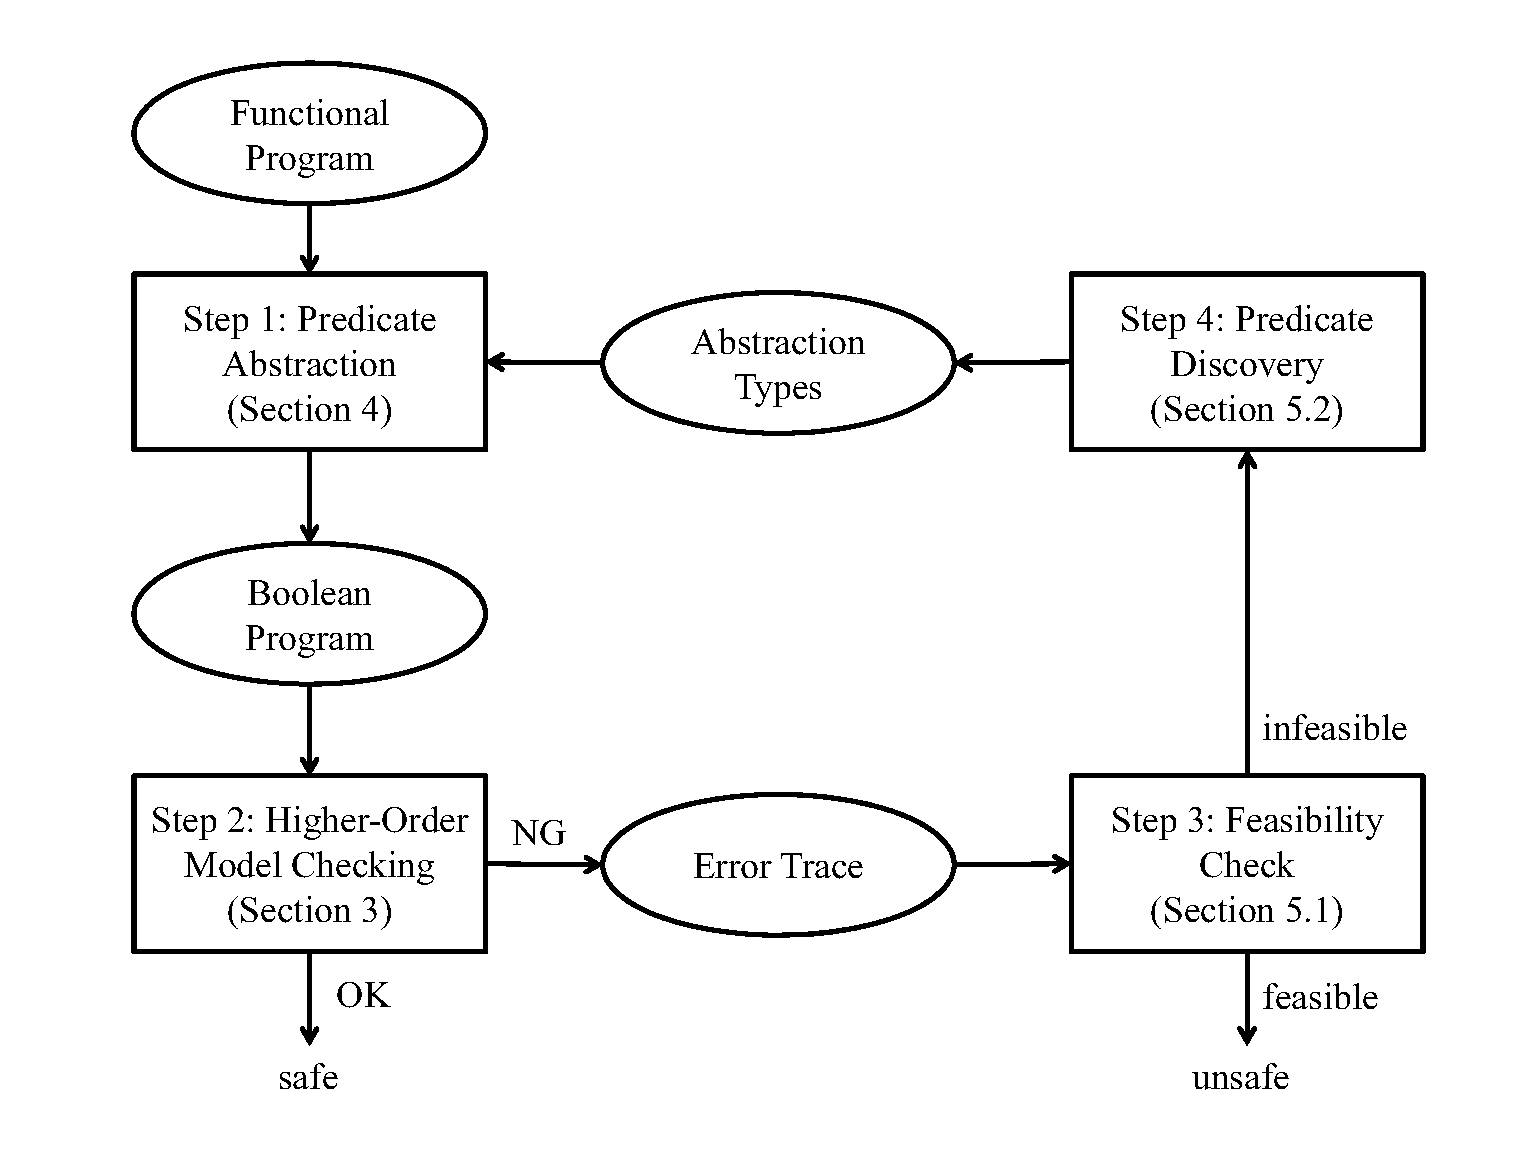
\includegraphics[scale=0.4]{overall.eps}
 \end{center}
\caption{Higher-Order Model Checking with Predicate Abstraction and CEGAR}
\label{fig:cegar}
\end{figure}

%The na\"{\i}ve application of the proposed approach, however, suffered
%from scalability problems, both in terms of efficiency and supported
%language features.  The verification framework supports infinite data
%domains other than integers.  However, we need interpolant theorem
%provers that can deal with the each infinite data domains (e.g., lists
%and trees).  Moreover, the verification framework does not support
%control operations (e.g., exceptions and call/cc).

%The na\"{\i}ve application of the proposed approach, however, suffered
%from scalability problems, both in terms of efficiency and supported
%language features.
%In this paper, we address the following
%problems of our previous work.
%\begin{enumerate}
% \item The previous framework requires an appropriate set of predicates for all
%       functions in the source program of predicate abstraction.
% \item Na\"{\i}ve CPS transformation extremely increases the computational cost
%       of model checking of higher-order boolean program because of the
%       increase of the order of the program.
% \item The previous framework does not support recursive data
%       structures like lists and trees.  Moreover, the previous
%       implementation does not support control operations like
%       exceptions and call/cc.
%\end{enumerate}
%
%We discuss each problem in more detail and explain our approach below.

In this paper, we address three problems of our previous work.
We discuss each problem and explain our approach below.

\begin{enumerate}
\item The main bottleneck of the previous version of MoCHi was the
      predicate abstraction and discovery (Steps 1 and 5), rather than
      higher-order model checking. Our previous method for predicate
      abstraction tried to abstract every integer argument of a function
      to a tuple of booleans.  As a result, verification of a program did
      not succeed until an appropriate set of predicates is found for
      \emph{every} function in the program.  For example, consider the
      program shown in Fig.~\ref{fig:sum}.  The program can be successfully
      verified if we abstract the program by using predicates
      $\Abs{y}{y \geq 0}$ for the second argument of \texttt{add} and
      $\Abs{r}{r \geq x}$ for the return value of \texttt{add} and
      \texttt{sum}.  The following is the
      abstracted program using the above predicates.

\begin{figure}[t]
\begin{alltt}
let add x y = x + y
let rec sum x = if x <= 0 then 0 else add x (sum (x-1))
let main x = assert (sum x >= x)
\end{alltt}
\caption{Example Program for Selective Predicate Abstraction}
\label{fig:sum}
\end{figure}
\begin{alltt}
let add () b = b
let rec sum () = if * then true
                else add (if sum () then true else *)
let main x = assert (sum ())
\end{alltt}
      Here, ``*'' means a non-deterministic boolean
      value.  The argument \texttt{b} denotes whether $\mathtt{y} \geq 0$ or not.
      Automatically finding all such appropriate predicates is
      difficult.  In the previous paper~\cite{KobayashiPLDI2011}, we
      have adapted CEGAR to find such predicates, but the technique is
      necessarily heuristic, and often fails.  If we abstract the
      program using only the predicate $\Abs{r}{r \geq x}$ for the return
      value of \texttt{sum}, we get the following abstracted program.
\begin{alltt}
let add () () = ()
let rec sum u = if * then true
                else let b = sum () and u = add () () in
                       *
let main x = assert (sum ())
\end{alltt}
      Since the return value of \texttt{add} is non-informative, the
      abstraction is too coarse.

      To reduce the burden to the predicate discovery phase, we introduce
      a refinement of predicate abstraction called \emph{selective
      predicate abstraction}.  As the name suggests, the selective
      predicate abstraction applies predicate abstraction to only a
      certain set of functions, and avoids abstraction of the other
      functions by inlining them.  The selective predicate abstraction
      generates the following safe program by using only the
      predicate $\Abs{r}{r \geq x}$ for the return values of \texttt{sum}
      and inlining \texttt{add}.
\begin{alltt}
let rec sum () = if * then true else if sum () then true else *
let main () = assert (sum ())
\end{alltt}
      In this way the selective predicate abstraction improves the
      precision of abstraction and reduce the cycle of CEGAR.

%%The first problem increases the number of CEGAR-cycle.
%To see the first problem, consider the following program.
%\begin{alltt}
%let add x y = x + y
%let rec sum x = if x < 0 then 0 else add x (sum (x-1))
%let main x = assert (sum x >= 0)
%\end{alltt}
%In our previous framework, we have to give predicate $\Abs{x}{x\geq0}$
%for return values of \texttt{sum}, return values of \texttt{add}, and
%arguments of \texttt{add}.  The following is the abstracted program
%using the predicate.
%\begin{alltt}
%let add bx by = if bx \&\& by then true else rand_bool()
%let rec sum _ = if rand_bool() then true
%                else add true (sum ())
%let main x = assert (sum ())
%\end{alltt}
%Here, \texttt{bx} is true and \texttt{bx} is true denote that
%$\mathtt{x} \geq 0$ and $\mathtt{y} \geq 0$, respectively.
%%If we abstract the program using predicate
%%$\Abs{x}{x\geq0}$ for return values of function \texttt{sum}, we get the
%%following abstracted program.
%%\begin{alltt}
%%let add u1 u2 = ()
%%let rec sum u = if rand_bool() then true
%%                else let b = sum () in
%%                     let u = add () () in
%%                       rand_bool()
%%let main x = assert (sum ())
%%\end{alltt}
%\texttt{rand\us{}bool()} means a non-deterministic boolean value.
%In fact, we can abstract the source program to the following program by
%using the definition of \texttt{add} with predicate $\Abs{x}{x\geq0}$
%only for return values of \texttt{sum}.
%\begin{alltt}
%let rec sum _ = if rand_bool() then true
%                else if sum () then true else rand_bool()
%let main x = assert (sum ())
%\end{alltt}
%In the body of \texttt{sum}, \texttt{add x (sum (x-1))}, i.e. \texttt{x
%+ sum (x-1)}, is abstracted to \texttt{if sum () then true else rand\us{}bool()}
%because $\mathtt{sum ()}$ is true denotes $\mathtt{sum (x-1)} \geq 0$.
%The case of $\mathtt{b}=\mathtt{false}$ is similar.
%We distinguish functions that are abstracted from functions that is not abstracted.
%In the example above, functions \texttt{sum} and \texttt{main} are abstracted, and
%function \texttt{add} is not abstracted.
%We abstract programs, intuitively, with extracting functions which is not abstracted.
%We formalize this abstraction, called selective predicate abstraction.

\item Another efficiency problem is caused by CPS transformation.  As
      stated above, our approach needs CPS transformation to resolve the
      gap between the evaluation strategies of higher-order recursion schemes and
      higher-order boolean programs.  However, CPS transformation increases the
      order\footnote{The order of program $t$ is the maximum order of
      the types of functions in $t$.  The order of type $\tau$ is
      defined by $\mathit{order}(\INT)=0$,
      $\mathit{order}(\TFun{\tau_1}{\tau_2}) =
      \mathit{max}(\mathit{order}(\tau_1)+1, \mathit{order}(\tau_2))$.}
      of programs and the growth of the order is not bounded by a constant.
      Since the complexity of model checking of higher-order recursion
      scheme is $n$-EXPTIME complete for order-$n$ recursion scheme, the
      increase of the order of an input is crucial to the verification
      time.
%
      For example, consider the following program.
\begin{alltt}
let rec check x f = f x; check (x+1) f
let f x = assert (x >= 0)
let main n = check n f
\end{alltt}
%Function \texttt{check} may cause an assertion failure only when two arguments are given.
      The above program is translated into the following program by
      a na\"{\i}ve call-by-value CPS transformation~\cite{Plotkin1975}.
\begin{alltt}
let rec check x k1 = k1 (\(\lambda\)f.\(\lambda\)k2.f x (\(\lambda\)_.check (x+1) (\(\lambda\)g.g f k2)))
let f x k = assert (x >= 0); k ()
let main n k = check n (\(\lambda\)g. g f k)
\end{alltt}
      To preserve the evaluation order of an original call-by-value program,
      each function of the translated call-by-name program takes
      a continuation and passes its return value to the continuation.  Note here that the
      order of the translated program is increased to 5.
%\begin{alltt}
%let check x k1 = k1 (\(\lambda\)y.\(\lambda\)k2. assert (x = y); k2 ())
%let main k = check (\(\lambda\)f. f n k)
%\end{alltt}
%let apply x k1 = k1 (\(\lambda\)f.\(\lambda\)k2. f x k2)
%let check x k1 = k1 (\(\lambda\)y.\(\lambda\)k2. assert (x = y); k2 ())
%let main n k = check n (\(\lambda\)f1. apply n (\(\lambda\)f2. f2 f1 k))
      We can, however, obtain the following order-3 program instead by omitting the continuation \texttt{k1} of \texttt{check},
      which is actually unnecessary since a partial application of \texttt{check} in the original program never causes side effects including an assertion failure.
\begin{alltt}
let rec check x f k = f x (\(\lambda\)_.check (x+1) f k)
let f x k = assert (x >= 0); k ()
let main n k = check n f k
\end{alltt}
%This transformation uses the fact that the application to the first
%argument does not cause an assertion failure and the context of
%\texttt{call n} is not required to have a continuation.
      Our CPS transformation avoids such unnecessary insertions of
      continuations.  We formalize this transformation, called
      \emph{selective CPS transformation}.

%Higher-order model checking (more precisely, the model
%checking of higher-order recursion schemes) has been studied
%recently~\cite{Ong2006}, and applied to verification of higher-order
%functional programs~\cite{KobayashiPOPL2009,KobayashiPLDI2011}.  Our
%previous framework~\cite{KobayashiPLDI2011} can verify higher-order
%programs.  The framework, however, cannot deal with recursive data
%structures, which are necessary for practical functional languages.
%Moreover, the na\"{\i}ve implementation based on the framework cannot
%verify large programs.
%
%In this paper, we introduce extensions and optimizations of the
%verification framework.  The extensions are language extensions to deal
%with recursive data structures (e.g., lists and trees) and control
%operators (e.g., exceptions and call/cc).  Our approach is to translate
%a source program written in the extended language to a program written
%in the previous language. This translation is sound and complete.

%The goal of the verification is to check
%that all assertions in a program never fail and pattern matching
%failures do not occur.

%\memo{The problem of the previous predicate abstraction}
%we introduce selective predicate abstraction as an optimization technique
%
%\memo{The problem of the previous model checking}
%we introduce selective CPS transformation as an optimization technique
%
%\memo{for language extension}
%(iii) functional encoding of recursive data structures and control operations to support a larger subset of ML.

\item The third problem is the insufficiency of supported language
      features.  Our previous framework requires an
      automated interpolating theorem prover for predicate abstraction and
      discovery, but practical provers are not available for recursive data
      structures like lists and trees. Thus, the implementation dealt with
      only integers as infinite data domains.
      
      To support recursive data structures without relying on interpolating
      theorem provers for them, we extend our verification framework as follows.
      As a preprocessing of our CEGAR-based model checking,
      we translate programs that manipulate recursive data structures into ones that manipulate only integers.
      The transformation is carried out by encoding recursive data structures using higher-order functions.  For example, a list is
      encoded to a function that maps an index $i$ to the $i$-th element.
      In a similar way, we support control operations (e.g., exceptions and call/cc) by using higher-order functions.
\end{enumerate}

%Our contributions are (i) the formalization of selective predicate
%abstraction using a simple but effective way to overcome the first
%efficiency problem, (ii) the formalization of selective CPS
%transformation to overcome the efficiency second problem, (iii) the
%formalization for language extension for recursive data structures
%(e.g., lists and trees) and control operations (e.g., exceptions and
%call/cc) that is sound, complete, and general for verification
%frameworks for higher-order language, and (iv) the implementation and
%experiments.

The rest of this paper is organized as follows. 
%In Sect.~\ref{sec:model-check}, we introduce our previous framework for
%higher-order programs with integers, which is the base of our framework
%described in this paper.
We first formalize the source language of verification in
Sect.~\ref{sec:language}.  Section~\ref{sec:opt} formalizes the
selective predicate abstraction and the selective CPS transformation.
Section~\ref{sec:extension} shows the language extensions for recursive
data structures and control operations.  Section~\ref{sec:experiments}
reports experiments.  Section~\ref{sec:related} discusses related work
and Sect.~\ref{sec:conclusion} concludes the paper.














%\section{Introduction}
%\label{sec:intro}
%[background]
%
%In this paper, we propose the verification method for program with
%recursive data types and control operator.  The goal of the verification
%is to check that a program does not execute the command \texttt{fail}.  We can
%also check that pattern matching failures and uncaught exceptions do not
%occur by a trivial transformation. For example, a program
%\texttt{(match t with ...)} cause a pattern match failure if and only if 
%a program \texttt{(match t with ... | \_ -> fail)} execute \texttt{fail}.
%
%The base of our framework is the verification of higher-order programs with integers.
%
%The idea of this framework is to translate a target program (with
%recursive data structures and exceptions) to a higher-order program with
%integers.  For example, the lists $[2;3;5]$ is encoded to a pair of the length $3$
%and a function $f$ such that $f(1)$, $f(2)$, $f(3)$ returns $2$, $3$,
%$5$, respectively.
%A function which takes lists and/or returns lists is encoded to
%a higher-order function which takes functions and/or returns functions.
%
%[Show running example of verifying a program with lists.]
%
%[discovering general predicates]
%
%[Show running example of discovering general predicates.]
%
%
%[the overview of this framework]
%
%We formalize the verification method for a language with lists.
%The verification for recursive data structures are argue in the Section ...
%
%The rest of this paper is organized as follows. We first formalize the
%target language in Section~\ref{sec:target-language}.  In
%Section~\ref{sec:model-check}, we introduce our previous framework for
%higher-order program with integers, which is the base of our framework
%described in this paper.  Section~\ref{sec:encoding} shows the program
%transformation which generate a program without lists from a program with lists,
%and argue about recursive data structures.
%Section~\ref{sec:control} shows that how to deal with control operators.
%Section~\ref{sec:discover}.
%Section~\ref{sec:experiments} reports preliminary experiments.
%Section~\ref{sec:related} discusses related work and
%Section~\ref{sec:conclusion} concludes the paper.
%

\section{Language}
\label{sec:lang}

This section introduces a simply-typed, higher-order functional language, 
which is used as the target of our verification method.

We assume a set \(\BT = \set{b_1,\ldots,b_n}\) of data types, and a set 
\(\vset{b_i}\) of constants, ranged over by \(c\), for each data type 
\(b_i\). We also assume that there are operators 
\(\OP:{b_{i_1},\ldots,b_{i_k}\ra b_j}\); we write \(\SEM{\OP}\) for the 
function denoted by \(\OP\). We assume that the set of data types 
includes \(\TUNIT\) with \(\vset{\TUNIT} = \tuple{}\), and \(\TBOOL\) 
with \(\vset{\TBOOL}=\set{\TRUE, \FALSE}\), and that the set of 
operators includes \(=\ :b,b\ra \TBOOL\) for every \(b\in \BT\), and 
boolean connectives such as \(\land:\TBOOL,\TBOOL\ra \TBOOL\).

The syntax of the language is given by:
\begin{eqnarray*}
D \mbox{ (program) }&::=& \set{f_1\ \seq{x}_1 = e_1,\ldots,f_m\ \seq{x}_m = e_m} \\
e \mbox{ (expressions) }
&::=& c \mid x\ \seq{v} \mid f\ \seq{v} \mid \LETEQIN{x}{e_1}{e_2} \mid \OP(\seq{v}) \\
&\mid& \FAIL \mid \ASSUME{v}{e} \mid \PAR{e_1}{e_2} \\ %%\mid \PARB{e_1}{e_2} \\
%%&\mid& (v_1,\dots,v_m) \mid \NTH{i}{v} \\
v \mbox{ (values) }&::=& c \mid x \mid f\ \seq{v} %\\ \mid (v_1,\dots,v_m) 
%%c&::=&n \mid \TRUE \mid \FALSE \mid \cdots \\
%%\OP&::=& + \mid \times \mid \ =\  \mid \NOT \mid \AND \mid \cdots \\
%%T&::=& B \mid T_1 \to T_2 \mid T_1 \times \dots \times T_n \\
%%B&::=& \TINT \mid \TBOOL \mid \cdots \\
%%E&::=& \HOLE \mid \LETEQIN{x}{E}{e}
\end{eqnarray*}

Here, \(\seq{x}\) abbreviates a (possibly empty) sequence 
\(x_1,\ldots,x_n\). In the definition \(f\ \seq{x} = e\), we call the 
length of \(\seq{x}\) the \emph{arity} of \(f\). In the definition of 
values, the length of \(\seq{v}\) in \(f\,\seq{v}\) must be smaller than 
the arity of \(f\). (In other words, \(f\,\seq{v}\) must be a partial 
application.) We assume that every function in \(D\) has a non-zero 
arity, and that \(D\) contains a distinguished function symbol 
\(\textit{main}\in \set{f_1,\ldots,f_m}\) whose simple type is 
\(\TUNIT\ra \TUNIT\).
%%of arity \(1\) that takes the unit value.

Most of the expressions are standard, except the following ones. The 
expression \(\FAIL\) aborts the program and reports a failure. The 
expression \(\ASSUME{v}{e}\) evaluates \(e\) if \(v\) is true; otherwise 
it stops the program (without a failure). The expression 
\(\PAR{e_1}{e_2}\) evaluates \(e_1\) or \(e_2\) in a non-deterministic 
manner. Note that a standard conditional expression 
\(\IFTE{v}{e_1}{e_2}\) can be expressed as: 
\[
 \PAR{(\ASSUME{v}{e_1})}{(\LETEQIN{x}{\NOT v}\ASSUME{x}{e_2})}.
\]
%
We can express the assertion \(\ASSERT{v}\) as 
\(\IFTE{v}{\tuple{}}{\FAIL}\).
%\[
% \PAR{(\ASSUME{v}{\tuple{}})}{(\ASSUME{\neg v}{\FAIL})}.
%\]
%
The random number generator \(\textit{randi}\) used in 
Section~\ref{sec:intro} is defined by:
\[
\begin{array}{l}
\textit{randi}\,\tuple{} = (\textit{randiFrom}\, 1)\PAROP (\textit{randiTo}\, 0)\\
\textit{randiFrom}\,n = n\PAROP (\textit{randiFrom}\,(n+1))\\
\textit{randiTo}\,n = n\PAROP (\textit{randiTo}\,(n-1))\\
\end{array}
\]

We assume that a program is well-typed in the standard simple type 
system, where the set of types is given by:
\[ \tau ::= b_1 \mid \cdots \mid b_n \mid \tau_1\ra \tau_2.\]
%
Furthermore, we assume that the body of each definition has a data type 
\(b_i\), not a function type. This is not a limitation, as we can always 
use the continuation-passing-style (CPS) transformation to transform a 
higher-order program to an equivalent one that satisfies the restriction.
%%%For example, a function definition
%%% f x = e
%%%(where e returns a function)
%%%can be transformed into
%%% f' x k = k e
%%%where k is the continuation parameter. This is indeed applied in our implementation.

%%%\(x\ \seq{v}\) and \(f\ \seq{v}\) are values if the arities of \(x\) and 
%%%\(f\) are less than the length of \(\seq{v}\). We write 
%%%\(\IFTE{e_1}{e_2}{e_3}\) for
%%%\[
%%% \PAR{(\ASSUME{e_1}{e_2})}{(\ASSUME{\NOT e_1}{e_3})}
%%%\]
%%%
%%%\todo{add explanation}

We define the set of \emph{evaluation contexts} by: \(E ::= \HOLE \mid 
\LETEQIN{x}{E}{e}\). The reduction relation is given in 
Figure~\ref{fig:opsem}. We label the reduction relation with 
\(0,1,\epsilon\) to record which branch has been chosen by a 
non-deterministic expression \(\PAR{e_1}{e_2}\); it will be used to 
relate reductions of a source program and an abstract program later in 
Sections~\ref{sec:pred} and \ref{sec:cegar}. We write \(e_1 
\redswith{l_1\cdots l_n}{D} e_2\) if 
\[e_1 (\redwith{\epsilon}{D})^* \redwith{l_1}{D}(\redwith{\epsilon}{D})^* \cdots (\redwith{\epsilon}{D})^* \redwith{l_n}{D}(\redwith{\epsilon}{D})^* e_2.\]
We often omit the subscript \(D\) when it is clear from the context.
%%\todo{add explanation}
The goal of our verification method is to check whether \\
\(\textit{main}\,\tuple{} \redswith{s}{D} \FAIL\).%
%%where \textit{main} is a function symbol with arity \(0\).
\footnote{Thus, we consider the reachability problem for a closed 
program. Note, however, that we can express unknown values by using 
non-determinism (recall \textit{randi}). It is also easy to extend our 
method to deal with more general verification problems, such as resource 
usage verification~\cite{Kobayashi2009}.}

\begin{figure}[t]
\typicallabel{E-Assume}
\infrule[E-App]
  {f\ \seq{x}=e \in D}
  {E[f\ \seq{v}] \stackrel{\epsilon}{\RED}_D E[[\seq{v}/\seq{x}]e]}
\rulesp

\infax[E-Let]
  {E[\LETEQIN{x}{v}{e}] \stackrel{\epsilon}{\RED}_D E[[v/x]e]}
\rulesp

\infax[E-Op]
  {E[\OP(\seq{c})] \stackrel{\epsilon}{\RED}_D E[\SEM{\OP}(\seq{c})]}
\rulesp

\infax[E-Par]
  {E[\PAR{e_0}{e_1}] \stackrel{i}{\RED}_D E[e_i]}
\rulesp

%%%\infax[E-Par-Right]
%%%  {\PAR{e_1}{e_2} \stackrel{1}{\RED}_D e_2}
%%%\rulesp
%%%
%%%\infax[E-Par2-Left]
%%%  {\PARB{e_1}{e_2} \stackrel{\epsilon}{\RED}_D e_1}
%%%\rulesp
%%%
%%%\infax[E-Par2-Right]
%%%  {\PARB{e_1}{e_2} \stackrel{\epsilon}{\RED}_D e_2}
%%%\rulesp

\infax[E-Assume]
  {E[\ASSUME{\TRUE}{e}] \stackrel{\epsilon}{\RED}_D E[e]}
\rulesp

%%\infax[E-Nth]
%%  {\NTH{i}{(v_1,\dots,v_m)} \stackrel{\epsilon}{\RED}_D v_i}
%%\rulesp

%\infrule[E-Ctx]
%  {e_1 \stackrel{l}{\RED}_D e_2}
%  {E[e_1] \stackrel{l}{\RED}_D E[e_2]}
%\rulesp

\infax[E-Fail]
  {E[\FAIL] \stackrel{\epsilon}{\RED}_D \FAIL}
%\rulesp

%%%\infax
%%%  {e \stackrel{\epsilon}{\RED^*}_D e}
%%%\rulesp
%%%
%%%\infrule
%%%  {e \stackrel{\pi_1}{\RED^*}_D e'' \andalso
%%%   e'' \stackrel{\pi_2}{\RED}_D e'}
%%%  {e \stackrel{\pi_1 \cdot \pi_2}{\RED^*}_D e'}
%%%\rulesp

\caption{Call-by-Value Operational Semantics}
\label{fig:opsem}
\end{figure}


\section{Higher-Order Boolean Programs and Model Checking}
\label{sec:boolean}

A source program is translated to a higher-order boolean program 
(abbreviated to HBP) by the predicate abstraction discussed in 
Section~\ref{sec:pred}. The language of HBP is essentially the same as 
the source language in the previous section, except:
\begin{asparaitem}
\item The set of data types consists only of types of the form 
\(\underbrace{\TBOOL\times \cdots \times \TBOOL}_m\) (which is 
identified with \(\TUNIT\) when \(m=0\), and \(\TBOOL\) when \(m=1\)). 
We assume there are the following operators to construct or deconstruct 
tuples:
\[
\begin{array}{rcl}
\tuple{\cdot,\ldots,\cdot}&:&{\TBOOL,\ldots,\TBOOL\ra \TBOOL\times \cdots \times\TBOOL}\\
\NTH{i}&:&{\TBOOL\times\cdots\times\TBOOL\ra \TBOOL}
\end{array}
\]
\item The set of expressions is extended with \(\PARB{e_1}{e_2}\) and 
unnamed functions \(\lambda x.e\). The former is used for expressing the 
non-determinism introduced by abstractions; it is the same as 
\(\PAR{e_1}{e_2}\), which is used to express the non-determinism present 
in a source program, except that the reduction is labelled with 
\(\epsilon\). This distinction is convenient for the CEGAR 
procedure discussed in Section~\ref{sec:cegar} to find a corresponding 
execution path of the source program from an execution path of the 
abstract program.
%
Unnamed functions are used just for technical convenience for defining 
predicate abstraction;
%%presenting predicate abstraction rules given in Section~\ref{sec:pred}; 
with \(\lambda\)-lifting, we can easily get rid of 
\(\lambda\)-abstractions. (The evaluation rules and evaluation contexts 
are accordingly extended with \(E[(\lambda x.e)v]\red E[[v/x]e]\) and 
\(E ::= \cdots \mid E\,e\mid v\,E\).)
\end{asparaitem}


The following theorem is the basis of our verification method. It 
follows immediately from the decidability of the model checking of 
higher-order recursion schemes~\cite{Ong2006}.
\begin{theorem}
\label{th:decidability}Let \(D\) be an HBP. The property \(\exists 
s.(\textit{main}\tuple{}\redswith{s}{D} \FAIL)\) is decidable.
\end{theorem}
We can use a recursion scheme model checker 
\trecs{}~\cite{Kobayashi2009,Kobayashi2009d} to decide the above 
property.\footnote{The gap between the operational semantics of our 
language and that of recursion schemes can be filled by the CPS 
transformation. Note also that finite state or pushdown model checkers 
cannot be used, as higher-order programs are in general strictly more 
expressive~\cite{Damm1982}.} If \(\exists 
s.(\textit{main}\tuple{}\redswith{s}{D} \FAIL)\) holds, the model 
checker generates an error path \(s\). The knowledge about recursion 
schemes is unnecessary for understanding the rest of this paper, but an 
interested reader may wish to consult 
\cite{Ong2006,Kobayashi2009,Kobayashi2009c}.
%%for higher-order recursion schemes and their connection to program verification.
%%how to reduce various verification problems for higher-order boolean programs into
%%model checking problems for higher-order recursion schemes.

\section{Predicate Abstraction}
\label{sec:pred}

This section formalizes predicate abstraction for higher-order programs.
%
As explained in Section~\ref{sec:intro}, we use \emph{abstraction types} 
to express which predicates should be used for abstracting each 
sub-expression. The syntax of abstraction types is given by:
\begin{eqnarray*}
\sigma \mbox{ (abstraction~types) }&::=& b_1[\seq{P}] \mid \cdots \mid b_n[\seq{P}] \mid x\COL\sigma_1 \to \sigma_2 \\
P,Q \mbox{ (predicates) }&::=& \lambda x.\psi \\
\Gamma \mbox{ (type~environments)} &::=& \emptyset \mid \Gamma,f\COL\sigma \mid \Gamma,x\COL\sigma
%\psi&::=& \NTH{i}{x} \mid \NOT \psi \mid \psi_1 \AND \psi_2
\end{eqnarray*}
Here, the meta-variable \(\psi\) represents an expression of type 
\(\TBOOL\) (which is called \emph{a formula}) that is constructed only 
from variables of base types, constants, and primitive operations; we do 
not allow formulas that contain function applications, like \(y>f(x)\).
%%We also use the meta-variable \(\psi\) to denote Boolean formulas (i.e, formulas that 
%%can be represented as Boolean expressions).
% we call the expressions of the Boolean progrms, Boolean expressions
%
% whose sub-expression can only have the type of the form \(\TBOOL\times 
%\cdots \times \TBOOL\). 
The base type \(b_i[\seq{P}]\) describes values \(v\) of type \(b_i\) 
that should be abstracted to a tuple of booleans
%that over-approximates 
\(\tuple{P_1(v),\dots,P_n(v)}\). For example, the integer \(3\) with the 
abstraction type \(\TINT[\lambda \nu.\nu>0,\lambda \nu.\nu<2]\) is 
abstracted to \(\tuple{\TRUE,\FALSE}\). We often abbreviate \(b[\,]\) 
to \(b\).
%(Recall again that it does not mean the value should satisfy \(\seq{P}\); an integer \(3\) can have type \(\TINT[\lambda x.x<0]\).)
The dependent function type \(x\COL\sigma_1 \to \sigma_2\) describes 
functions that take a value \(v\) of type \(\sigma_1\), and return a 
value of type \([v/x]\sigma_2\).
% if applied to the actual argument \(v\) of type \(\sigma_1\).
The scope of \(x\) in the type \(x\COL\sigma_1 \to \sigma_2\) is 
\(\sigma_2\). When \(x\) does not occur in \(\sigma_2\), we often write 
\(\sigma_1\to\sigma_2\) for \(x\COL\sigma_1 \to \sigma_2\).
%
%In the function type, the variable \(x\) denotes the actual argument, 
%and can be used in the predicates in \(\sigma_2\).
As mentioned already, abstraction types only describe how each 
expression should be abstracted, not the actual value. For example, \(3\) 
can have type \(\INT[\lambda \nu.\nu<0]\), and \(\lambda x.x\) can have 
type \(x\COL\INT[\,] \ra \INT[\lambda \nu.\nu=x+1]\) (and abstracted to
%%a function 
\(\lambda x:\TUNIT.\FALSE\)).

We do not consider types whose predicates are ill-typed or violate a 
variable's scope, such as \(x\COL\TBOOL[\,]\to \TINT[\lambda y.x+1=y]\) 
and \(x\COL\TINT[\lambda x.y>x]\to y\COL\TINT[\,]\to \TBOOL[\,]\). (The 
former uses a boolean variable as an integer, and the latter refers to 
the variable \(y\) outside its scope.) Figure~\ref{fig:wf} defines the 
well-formedness conditions for types and type environments. In the 
figure, \(\Delta\pS e:\tau\) denotes the type judgment of the standard 
simple type system. We write \(\alphaB(\sigma)\) and \(\alphaB(\Gamma)\) 
respectively for the simple type and the simple type environment 
obtained by removing predicates. For example, 
%%\begin{eqnarray*}
%%&&
\(\alphaB(f\COL (x\COL\TINT[\,]\to \TINT[\lambda y.y>x]), z\COL\TINT[\lambda z.z>0]) %%\\
  = f\COL \TINT \to \TINT,z\COL \TINT\).
%%  &=& f\COL \TINT \to \TINT,z\COL \TINT.
%%\end{eqnarray*}
\begin{figure}
\infrule{
    \alphaB(\Gamma),x\COL b \pS \psi_i: \TBOOL \mbox{ for each $i\in\set{1,\ldots,n}$}}
   {\Gamma \pW b[\lambda x.\psi_1,\ldots, \lambda x.\psi_n]}
\rulesp
\InfruleW{0.45}{\Gamma \pW \sigma_1 \andalso \Gamma, x\COL\sigma_1 \pW \sigma_2}
   {\Gamma \pW x\COL\sigma_1 \to \sigma_2}
\InfruleW{0.15}{\ }{\pW \emptyset}
\InfruleW{0.25}{\pW \Gamma \andalso \Gamma \pW \sigma}
      {\pW \Gamma, x\COL\sigma}
\caption{Well-formed types and type environments}
\label{fig:wf}
\end{figure}


Figure~\ref{fig:pred_abst} defines the predicate abstraction relation 
\(\T{\Gamma}{e_1}{\sigma}{e_2}\), which reads that an expression \(e_1\) 
(of the source language in Section~\ref{sec:lang}) can be abstracted to 
an expression \(e_2\) (of the HBP language given in 
Section~\ref{sec:boolean}) by using the abstraction type \(\sigma\), 
under the assumption that each free variable \(x\) of \(e_1\) has been 
abstracted using the abstraction type \(\Gamma(x)\). In the rules, it is 
implicitly assumed that all the type environments and types are 
well-formed. We do not distinguish between function variables and other 
variables (hence, \rn{A-App} applies also to a function variable \(f\)).
%%The predicate abstraction relation \(\T{\Gamma}{e_1}{\sigma}{e_2}\) 
%%reads that the Boolean expression \(e_2\) is an abstraction of the 
%%expression \(e_1\) with the abstraction type \(\sigma\) under 
%%the 
%%abstraction type environment \(\Gamma\).
%
%%The derivation rules for the relation are presented in 
%
%The rules are .. the previous dependent type 
%systems~\cite{Flanagan2006,Rondon2008,Unno2009,Terauchi2010} except that 
%...
%
%In \rn{A-Var}, we write \(x\ \seq{e}\) for \(\LETEQIN{\seq{x}}{\seq{e}}{x\ \seq{x}}\).
%In \rn{A-Fun}, we write \(f\ \seq{e}\) for \(\LETEQIN{\seq{x}}{\seq{e}}{f\ \seq{x}}\).
%\rn{A-Assume} and 
In \rn{A-CAdd}, \(\ASSUME{e_1}{e_2}\) is a syntax sugar for 
\(\LETEQIN{x_1}{e_1}{\ASSUME{x_1}{e_2}}\).

\begin{figure}[tbp]
\typicallabel{A-Assume}

%%%\infrule[A-Const]
%%%  {c\mbox{~has~the~base~type~}b}
%%%  {\T{\Gamma}{c}{b[\lambda x.x=c]}{\TRUE}}
%%%\rulesp
%%%
%%%\infrule[A-Op]
%%%  {\alphaB(\Gamma) \pS \OP(\seq{v}):b}
%%%  {\T{\Gamma}{\OP(\seq{v})}{b[\lambda x.x=\OP(\seq{v})]}{\TRUE}}
%%%\rulesp
%%%
%%%
%%%\infrule[A-Var]
%%%  {x:b[\seq{P}] \in \Gamma}
%%%  {\T{\Gamma}{x}{b[\lambda y.y=x]}{\TRUE}}
%%%\rulesp


\infrule[A-Base]
  {\mbox{$e$ is a constant, a variable or an expression of the form \(\OP(\seq{v})\)}\\
    \alphaB(\Gamma) \pS e \COL b}
  {\T{\Gamma}{e}{b[\lambda \nu.\nu=e]}{\TRUE}}
\rulesp

\infrule[A-CAdd]
  {\T{\Gamma}{e}{b[\seq{Q}]}{e'} \\
   \beta(\Gamma,x:b[\seq{Q}]) \pS \psi \COL \TBOOL \andalso
   \beta(\Gamma,x:b[\seq{Q}]) \pS \psi' \COL \TBOOL \\
   \models  P(x) \IMPLY \THE{\Gamma,x:b[\seq{Q}]}(\psi) \andalso
   \models \neg P(x) \IMPLY \THE{\Gamma,x:b[\seq{Q}]}(\psi') \\
   e''=\PARB{(\ASSUME{\psi}{\TRUE})}{(\ASSUME{\psi'}{\FALSE})}}
  {\T{\Gamma}{e}{b[\seq{Q},P]}{\LETEQIN{x}{e'}{\tuple{x,e''}}}}
\rulesp

\infrule[A-CRem]
  {\T{\Gamma}{e}{b[\seq{Q},\seq{P}]}{e'}}
  {\T{\Gamma}{e}{b[\seq{P}]}{\LETEQIN{\tuple{\seq{x},\seq{y}}}}{e'}{\tuple{\seq{y}}}}
\rulesp

\infrule[A-App]
  {\Gamma(x)=(y_1\COL\sigma_1 \to \cdots \to y_k\COL\sigma_k \to\sigma) \\
%% \andalso   \mbox{\(\Gamma(x)\) is a function type} \\
    \T{\Gamma,y_1:\sigma_1,\dots,y_{i-1}:\sigma_{i-1}}{v_i}{[v_1/y_1,\ldots,v_{i-1}/y_{i-1}]\sigma_i}{e_i}\\
  \mbox{ (for each $i\in\set{1,\ldots,k}$)}}
  {\T{\Gamma}{x\ \seq{v}}{[\seq{v}/\seq{y}]\sigma}
     {\begin{array}{l}
      \LETEQIN{y_1}{e_1}\cdots \\
      \LETEQIN{y_k}{e_k}x\ \seq{y}
      \end{array}}}
\rulesp
%%%
%%%\infrule[A-Fun]
%%%  {f:(\seq{x}:\seq{\sigma} \to \sigma) \in \Gamma \andalso
%%%   \T{\Gamma}{\seq{v}}{\seq{\sigma}}{\seq{e}}}
%%%  {\T{\Gamma}{f\ \seq{v}}{[\seq{v}/\seq{x}]\sigma}{f\ \seq{e}}}
%%%\rulesp

\infrule[A-Let]
  {\T{\Gamma}{e_1}{\sigma'}{e_1'} \andalso
   \T{\Gamma,x:\sigma'}{e_2}{\sigma}{e_2'}}% \andalso
%   x \not\in \FV{\sigma}}
  {\T{\Gamma}{\LETEQIN{x}{e_1}{e_2}}{\sigma}{\LETEQIN{x}{e_1'}{e_2'}}}
\rulesp


\infrule[A-Fail]
  {\beta(\Gamma) \pS \psi \COL \TBOOL \andalso
   \models \THE{\Gamma}(\psi)}
  {\T{\Gamma}{\FAIL}{\sigma}{\ASSUME{\psi}{\FAIL}}}
\rulesp

\infrule[A-Asm]
  {\T{\Gamma}{v}{\TBOOL[\lambda x.x]}{e_1} \\
   \T{\Gamma,x\COL\TBOOL[\lambda x.v]}{e}{\sigma}{e_2}}
  {\T{\Gamma}{\ASSUME{v}{e}}{\sigma}{\LETEQIN{x}{e_1}\ASSUME{x}{e_2}}}
\rulesp

\infrule[A-Par]
  {\T{\Gamma}{e_1}{\sigma}{e_1'} \andalso
   \T{\Gamma}{e_2}{\sigma}{e_2'}}
  {\T{\Gamma}{\PAR{e_1}{e_2}}{\sigma}{\PAR{e_1'}{e_2'}}}
\rulesp

%\infrule[A-Par2]
%  {\T{\Gamma}{e_1}{\sigma}{e_1'} \andalso
%   \T{\Gamma}{e_2}{\sigma}{e_2'}}
%  {\T{\Gamma}{\PARB{e_1}{e_2}}{\sigma}{\PARB{e_1'}{e_2'}}}
%\rulesp

%\infrule[A-Tuple]
%  {\T{\Gamma}{v_i}{\sigma_i}{e_i} \andalso
%   (\mbox{for~each~}i=1,\dots,m)}
%  {\T{\Gamma}{(v_1,\dots,v_m)}{\sigma_1 \times \dots \times \sigma_m}{(e_1,\dots,e_m)}}
%\rulesp
%
%\infrule[A-Nth]
%  {\T{\Gamma}{v}{\sigma_1 \times \dots \times \sigma_m}{e}}
%  {\T{\Gamma}{\NTH{i}{v}}{\sigma_i}{\NTH{i}{e}}}
%\rulesp


\infrule[A-CFun]
  {\T{\Gamma}{e}{(x\COL\sigma'_1\to\sigma'_2)}{e'}
  \andalso \T{\Gamma,x\COL\sigma_1}{x}{\sigma'_1}{e_1'}
  \\ \T{\Gamma,x\COL\sigma_1,x'\COL\sigma'_1,y\COL\sigma'_2}{y}{\sigma_2}{e_2'}}
  {\T{\Gamma}{e}{(x\COL\sigma_1\to\sigma_2)}
   {\begin{array}{l}
    \LETEQIN{f}{e'} \\
    \lambda x.\LETEQIN{x'}{e_1'} \\
    \ \ \ \ \ \ \LETEQIN{y}{f\ x'}e_2'\end{array}}}

\rulesp

\infrule[A-Prog]
  {f_i: (\seq{x}_i:\seq{\sigma}_i \to \sigma_i) \in \Gamma \andalso
   \T{\Gamma,\seq{x}_i:\seq{\sigma}_i}{e_i}{\sigma_i}{e_i'} \\
   \mbox{(for each \(i \in \set{1,\dots,m}\))} \andalso
   \Gamma(\textit{main})=\TUNIT[\,] \to \TUNIT[\,]}
  {\T{}{\set{f_1\ \seq{x}_1 = e_1,\ldots,f_m\ \seq{x}_m = e_m}}{\Gamma}{\\\set{f_1\ \seq{x}_1 = e_1',\ldots,f_m\ \seq{x}_m = e_m'}}}
%%\koba{Do we need somewhere the condition that the abstraction types conform to the simple types?}
\caption{Predicate Abstraction Rules}
\label{fig:pred_abst}
\end{figure}


In \rn{A-CAdd} and \rn{A-Fail}, \(\beta(\sigma)\) (\(\beta(\Gamma)\), 
resp.) represent the simple type (simple type environment, resp.) 
obtained by replacing each occurrence of a base abstraction type 
\(b[P_1,\dots,P_m]\) with \(\underbrace{\TBOOL \times \cdots \times 
\TBOOL}_m\). Intuitively, \(\beta(\Gamma)\) represents the type 
environment for the output program of the transformation. 

%%Similar syntax sugars are also used in \rn{A-Assume} and \rn{A-Coerce}.
%%%In \rn{A-Assume} and \rn{A-Coerce}, we write \(\ASSUME{e_1}{e_2}\) for:
%%%\[
%%% \LETEQIN{x}{e_1}{\ASSUME{x}{e_2}}.
%%%\]
%%%In \rn{A-Coerce}, we write \(\tuple{e_1,\dots,e_n}\) for:
%%%\[
%%% \LETEQIN{x_1}{e_1}{\dots \IN\ \LETEQIN{x_n}{e_n}{\tuple{x_1,\dots,x_n}}}.
%%%\]
%




We explain the main rules. 
Base values are abstracted by using three rules \rn{A-Base}, \rn{A-CAdd}, and \rn{A-CRem}.
Before explaining those rules, 
let us discuss the following simplified version, specialized
for a single predicate:
\infrule[A-BSimp]
  {
%%\mbox{$e$ is a constant, a variable or an expression of the form \(\OP(\seq{v})\)}\\
%%    \alphaB(\Gamma) \pS e \COL b\\
%%   \beta(\Gamma,x:b[\seq{Q}]) \pS \psi \COL \TBOOL \andalso
%%   \beta(\Gamma,x:b[\seq{Q}]) \pS \psi' \COL \TBOOL \\
   \models  P(e) \IMPLY \THE{\Gamma}(\psi) \andalso
   \models \neg P(e) \IMPLY \THE{\Gamma}(\psi')}
  {\T{\Gamma}{e}{b[P]}{\PARB{(\ASSUME{\psi}{\TRUE})}{(\ASSUME{\psi'}{\FALSE})}}}

\noindent
Here, we assume that \(e\) is a constant, a variable, or an expression of the form \(\OP(\seq{v})\)
and has a base type \(b\). \(\psi\) and \(\psi'\) are boolean formulas that may contain variables in \(\Gamma\).
As \(e\) may contain variables, we need to take into account information about the values of the variables,
which is obtained by using the substitution \(\THE{\Gamma}\), defined as:
%%\begin{eqnarray*}
\(\set{x \mapsto \tuple{P_1(x),\dots,P_m(x)} \mid \Gamma(x)=b[P_1,\dots,P_m]}\).
%%\end{eqnarray*}
For example, let \(\Gamma\) be \(x\COL\TINT[\lambda x.x\mathbin{>}0, \lambda x.x<0]\)
and \(\psi\) be \(\NTH{1}(x) \land \NTH{2}(x)\). Then,
\(\THE{\Gamma}(\psi) = x>0\land x<0\).
As in this example, the substitution \(\THE{\Gamma}\) maps a boolean expression of an abstract program
to the corresponding condition in the source program.
In rule \rn{A-BSimp} above, \(\models  P(e) \IMPLY \THE{\Gamma}(\psi)\) means that
\(P(e)\) is true only if \(\THE{\Gamma}(\psi)\) is true, i.e. the value of \(\psi\) in the abstract program is true.
Thus, the abstract value of \(e\) may be \(\TRUE\) only if the value of \(\psi\) is \(\TRUE\),
hence the part \(\ASSUME{\psi}{\TRUE}\) in the abstract program. Similarly,
the abstract value of \(e\) may be \(\FALSE\) only if the value of \(\psi'\) is \(\TRUE\),
hence the part \(\ASSUME{\psi'}{\FALSE}\).

For example, let \(e \equiv x+1\),  \(P \equiv \lambda x\geq 0\), and \(\Gamma \equiv x\COL \TINT[P]\).
Then, \(\models P(x+1) \imply \TRUE\) and \(\models \neg P(x+1) \imply \neg P(x)\), so that 
\(e\) is abstracted to \(\PARB{(\ASSUME{\TRUE}{\TRUE})}{(\ASSUME{\neg x}{\FALSE})}\).
Note that \(\THE{\Gamma}(\neg x) = [P(x) /x] \neg x = \neg P(x)\).

We need to generalize the above rule to the case for multiple predicates.
The following is a naive rule.
\infrule[A-BCartesian]
  {\T{\Gamma}{e}{b[P_i]}{e_i}}
  {\T{\Gamma}{e}{b[P_1,\ldots,P_n]}{\tuple{e_1,\ldots,e_n}}}
This produces a well-known cartesian abstraction, which is often too imprecise.
The problem is that each boolean value of the abstraction is computed separately,
ignoring the correlation. 
For example, let \(P_1 \equiv \lambda x.x>0\) and
\(P_2 \equiv \lambda x.x \leq 0\) with \(n=2\). Then, a possible abstraction of an unknown integer
should be \(\tuple{\TRUE,\FALSE}\) and \(\tuple{\FALSE,\TRUE}\), but the above
rule would generate 
\(\tuple{(\PARB{\TRUE}{\FALSE}),(\PARB{\TRUE}{\FALSE})}\), which also contains
\(\tuple{\TRUE,\TRUE}\) and \(\tuple{\FALSE,\FALSE}\).

The discussion above motivated us to introduce the three rules 
\rn{A-Base}, \rn{A-CAdd}, and \rn{A-CRem}. 
In order to abstract an expression \(e\) with \(b[P_1,\ldots,P_n]\),
we first use \rn{A-Base} to abstract \(e\) to \(\TRUE\) by using the abstraction type \(b[\lambda \nu.\nu=e]\);
this is necessary to keep the exact information about \(e\) during the computation of abstractions.
\rn{A-CAdd} is then used to add predicates \(P_1,\ldots,P_n\) one by one, taking into account
the correlation between the predicates. Note that in \rn{A-CAdd}, 
the result of abstraction by the other predicates is taken into account by the substitution \(\THE{\Gamma,x:b[\seq{Q}]}\).
Finally, \rn{A-CRem} is used to remove the unnecessary predicate \(\lambda \nu.\nu=e\).
See Example~\ref{ex:abstraction} for an application of these rules.

Note that rule \rn{A-CAdd} is non-deterministic in the choice of 
conditions \(\psi\) and \(\psi'\), so that how to compute the conditions 
is left unspecified. We have intentionally made so, because depending on 
base data types, the most precise conditions (the strongest conditions 
entailed by \(P(x)\) and \(\neg P(x)\)) may not be computable or are too 
expensive to compute. For linear arithmetics, however, we can use 
off-the-shelf automated theorem provers to obtain such conditions.

%
%%%In the rule \rn{A-Base}, a base value \(e\) 
%%%is abstracted to \(\TRUE\), by using the equality predicate \(\lambda 
%%%x.x=e\). Note that \(e\) is restricted to a constant, a variable, or a 
%%%primitive operation, so that \(x=e\) is a formula. To abstract base 
%%%values with other predicates, the rules \rn{A-CAdd} and \rn{A-CRem} 
%%%explained later should be used.
%%%%
%%%%
%%%%%\nk{We may want to consider merging \rn{A-Const} and \rn{A-Op}. 
%%%%%In fact, a constant \(c\) can be considered a nullary operator.}
%%%%

In rule \rn{A-App}, each argument \(v_i\) is abstracted by using the 
abstraction type \(\sigma_i\) with \(y_1,\ldots,y_{i-1}\) being replaced 
by the actual arguments. 
%%For example, we can derive:
%%\[
%% \T{\Gamma}{\texttt{inc}\ y}{\TINT[\lambda \nu.\nu=y+1]}{\texttt{inc}\ y}.
%%\]
%%for \(\Gamma=\texttt{inc}:(x:\TINT[\,] \to \TINT[\lambda \nu.\nu=x+1]),y:\TINT[\,]\).
%%%
Note that this rule applies also to the case where the sequence 
\(\seq{v}\) is empty (i.e. \(k=0\)). Thus, we can derive 
\(\T{\Gamma}{y}{\sigma}{y}\) if \(\Gamma(y)=\sigma\). Note also that the 
boolean expression \(e_i\) in \rn{A-App} can depend on 
\(y_1,\dots,y_{i-1}\).

%%In \rn{A-Fail}, we write \(\beta(\sigma)\) (\(\beta(\Gamma)\), resp.) 
%%for the simple type (simple type environment, resp.) obtained by 
%%replacing each occurrence of a base abstraction type \(b[P_1,\dots,P_m]\) 
%%with \(\underbrace{\TBOOL \times \cdots \times \TBOOL}_m\). Intuitively, 
%%\(\beta(\Gamma)\) represents the type environment for the output program 
%%of the transformation. 
%
In \rn{A-Fail}, the assume statement is inserted for filtering out an 
invalid combination of abstract values. For example, let \(\Gamma\) be 
\(x\COL\TINT[\lambda x.x\mathbin{>}0, \lambda x.x<0]\). Then, 
\(\ASSUME{(\NTH{1}(x) \land \NTH{2}(x))}\) is inserted since \(x>0\) and 
\(x<0\) cannot be true simultaneously.
%
In \rn{A-Asm}, we can use the fact that \(v\) is \(\TRUE\) in \(e\) for 
abstracting \(e\).

%%%The rules \rn{A-CAdd} and \rn{A-CRem} are used for coercing the 
%%%abstraction type of a base expression. Before explaining them, let us 
%%%first explain the following straightforward coercion rule:
%%%%
%%%\infrule
%%%  {\T{\Gamma}{e}{b[\seq{Q}]}{e'} \\
%%%   \beta(\Gamma,x:b[\seq{Q}]) \pS \psi_i \COL \TBOOL \andalso
%%%   \beta(\Gamma,x:b[\seq{Q}]) \pS \psi_i' \COL \TBOOL \\
%%%   \models P_i(x) \IMPLY \THE{\Gamma,x:b[\seq{Q}]}(\psi_i) \andalso
%%%   \models \neg P_i(x) \IMPLY \THE{\Gamma,x:b[\seq{Q}]}(\psi_i') \\
%%%   e_i=\PARB{(\ASSUME{\psi_i}{\TRUE})}{(\ASSUME{\psi_i'}{\FALSE}) \\
%%%   \mbox{(for each \(i \in \set{1,\dots,n}\))}}}
%%%  {\T{\Gamma}{e}{b[P_1,\dots,P_n]}{\LETEQIN{x}{e'}\tuple{e_1,\dots,e_n}}}
%%%%
%%%In the rule, the first premise means that \(e\) is abstracted to \(e'\) 
%%%by using predicates \(\seq{Q}\). To coerce the abstraction type of \(e\) 
%%%to \(b[P_1,\dots,P_n]\), we over-approximate the possible value of 
%%%\(P_i(e)\) for each \(i \in \set{1,\dots,n}\), by using \(e'\). Note 
%%%that the most imprecise abstraction is \(\PARB{\TRUE}{\FALSE}\), which 
%%%represents a non-deterministic boolean. To get a more precise 
%%%abstraction, we find a condition \(\THE{\Gamma,x:b[\seq{Q}]}(\psi_i)\) 
%%%(\(\THE{\Gamma,x:b[\seq{Q}]}(\psi_i')\), resp.) that is entailed by 
%%%\(P_i(x)\) (\(\neg P_i(x)\), resp.) and expressed by using only 
%%%available predicates, where \(x\) represents the value of \(e\). By 
%%%using them, we obtain a more precise abstraction of \(P_i(x)\):
%%%\[\PARB{(\ASSUME{\psi_i}{\TRUE})}{(\ASSUME{\psi_i'}{\FALSE})}.\]
%%%%
%%%For example, suppose that we have \(\T{\Gamma}{e}{\TINT[\lambda 
%%%x.x=1]}{e'}\). The abstraction \(e'\) represents whether \(e=1\) holds. 
%%%%
%%%To change the abstraction type to \(\TINT[\lambda x.x>0]\), we look for 
%%%boolean formulas \(\psi\) and \(\psi'\) such that \(\THE{\Gamma,x\COL 
%%%b[\lambda x.x=1]}(\psi)\) and \(\THE{\Gamma,x\COL b[\lambda 
%%%x.x=1]}(\psi')\) are entailed by \(x>0\) and \(\neg(x>0)\) respectively, 
%%%and obtain \(\psi = \TRUE\) and \(\psi' = \neg x\) since we have
%%%\begin{eqnarray*}
%%%&&\models x > 0 \implies \TRUE(\equiv\THE{\Gamma,x\COL b[\lambda x.x=1]}(\psi)), \\
%%%&&\models x \leq 0 \implies x \neq 1(\equiv\THE{\Gamma,x\COL b[\lambda x.x=1]}(\psi')).
%%%\end{eqnarray*}
%%%%
%%%As a result, we obtain:
%%%%
%%%\[\T{\Gamma}{e}{\TINT[\lambda x.x>0]}{\LETEQIN{x}{e'}{\tuple{e''}}}.\]
%%%%
%%%where \(e'' = \PARB{(\ASSUME{\TRUE}\TRUE)}{(\ASSUME{\neg x}\FALSE)}\). 
%%%%
%%%%For example, let us consider how the expression \(x+1\) is abstracted by 
%%%%using the abstraction type \(\TINT[\lambda \nu.\nu>0]\) under the type 
%%%%environment \(x:\TINT[\lambda \nu.\nu=0]\). We look for boolean formulas 
%%%%\(\psi_1\) and \(\psi_1'\) such that \(\THE{x:\TINT[\lambda 
%%%%\nu.\nu=0]}(\psi_1)\) and \(\THE{x:\TINT[\lambda \nu.\nu=0]}(\psi_1')\) 
%%%%are entailed by \(x+1>0\) and \(\neg(x+1>0)\) respectively, and obtain 
%%%%\(\psi_1 = \TRUE\) and \(\psi_1' = \neg x\) since we have
%%%%\begin{eqnarray*}
%%%%&&\models x+1 > 0 \implies \TRUE(\equiv\THE{x:\TINT[\lambda \nu.\nu=0]}(\psi_1)), \\
%%%%&&\models x+1 \leq 0 \implies x \neq 0(\equiv\THE{x:\TINT[\lambda \nu.\nu=0]}(\psi_1')).
%%%%\end{eqnarray*}
%%%%As a result, we obtain:
%%%%\[\T{x:\TINT[\lambda x.x=0]}{x+1}{\TINT[\lambda x.x>0]}{e'}.
%%%%\]
%%%%Here, \(e' = \PARB{(\ASSUME{\TRUE}\TRUE)}{(\ASSUME{\neg x}\FALSE)}\).
%%%%
%%%
%%%Note that the above coercion rule may cause imprecise abstraction even 
%%%if we use the most precise boolean formulas for \(\psi_i\) and 
%%%\(\psi_i'\). It is because the boolean expression \(e_i\) for each 
%%%predicate \(P_i\) is obtained without considering \(e_j\ (j \neq i)\) 
%%%for other predicates \(P_j\). For example, we get an imprecise boolean 
%%%expression \(\tuple{\PARB{\TRUE}{\FALSE},\PARB{\TRUE}{\FALSE}}\) if we 
%%%coerce the type \(\TINT[\,]\) of some expression to \(\TINT[\lambda 
%%%\nu.\nu>0,\lambda \nu.\nu<0]\). (Note here that the second predicate 
%%%must be false if the first predicate is true.)
%%%
%%%To avoid the imprecision, we instead use \rn{A-CAdd} to add predicates 
%%%one-by-one considering other ones, and then use \rn{A-CRem} to remove 
%%%unnecessary ones.
%%%%
%%%For example, given \(\T{\Gamma}{e}{\TINT[\,]}{e_0}\), we can use 
%%%\rn{A-CAdd} and \rn{A-CRem} to derive:
%%%\begin{eqnarray*}
%%%\T{\Gamma}{e}{\TINT[\lambda \nu.\nu>0,\lambda \nu.\nu<0]}{e_1}
%%%\end{eqnarray*}
%%%Here, \(e_1 \equiv \LETEQIN{x_1}{\PARB{\TRUE}{\FALSE}}e_2\) and \(e_2\) 
%%%is:
%%%\[
%%% \tuple{x_1,\IFTE{x_1}{\FALSE}{\PARB{\TRUE}{\FALSE}}}.
%%%\]
%%%%
%%%%%As the former is the most tricky rule, we explain it in detail.
%%%%%In the rule, \(\THE{\Gamma}\) represents the following substitution:
%%%%%\begin{eqnarray*}
%%%%%\set{x \mapsto \tuple{P_1(x),\dots,P_m(x)} \mid \Gamma(x)=b[P_1,\dots,P_m]}.
%%%%%\end{eqnarray*}
%%%%%%Given a Boolean formula \(\psi\) whose variables are in \(\DOM{\Gamma}\), 
%%%%%%we can regard the formula \(\THE{\Gamma}\psi\) as a \emph{concretization} 
%%%%%%of \(\psi\) with \(\Gamma\), by interpreting each variable \(x\) in 
%%%%%%\(\psi\) as the tuple \(\tuple{P_1(x),\dots,P_m(x)}\).
%%%%%% of the predicates for \(x\) specified by \(\Gamma\).
%%%%, which has the type \(\underbrace{\TBOOL \times \cdots \times 
%%%%\TBOOL}_n\)
%%%
%%%%
%%%%\addspan{A-Base is NOT subsumed by A-CADD. For example, there is no way 
%%%%to derive \(\T{\Gamma}{1}{\INT[\lambda x.x=1]}{\TRUE}\) without using 
%%%%\rn{A-Base}. (Note also that the first premise of A-CADD rule must have 
%%%%originally been derived from A-Base.)}

Rule \rn{A-CFun} is used for changing the abstraction type of a function 
from \(x\COL\sigma_1\ra \sigma_2\) to \(x\COL\sigma'_1\ra \sigma'_2\), 
which is analogous to the usual rule for subtyping-based coercion. If a 
function \(f\) is used in different contexts which require different 
abstraction types of \(f\), \rn{A-CFun} can be used to adjust the 
abstraction type of \(f\) to that required for each context.

%%%\begin{example}
%%%\label{ex:cfun}
%%%\addspan{Let \(\Gamma=f:(x:\TINT \to \TINT[\lambda \nu.\nu=x+1])\). 
%%%Suppose that in some context, \(f\) is required to have the abstraction 
%%%type \(\TINT[\lambda \nu.\nu \geq 0] \to \TINT[\lambda \nu.\nu \geq 0]\). 
%%%Predicate abstraction of \(f\) in the context proceeds as in Figure~\ref{fig:cfun}.}
%%%\end{example}

%%%\begin{figure*}
%%%\[
%%%\infers[A-CFun]
%%% {\T{\Gamma}{f}{\TINT[\lambda \nu.\nu \geq 0] \to \TINT[\lambda \nu.\nu \geq 0]}{e}}
%%% {\infers%[A-App]
%%%   {\T{\Gamma}{f}{\sigma}{f}}
%%%   {\Gamma(f)=\sigma} \andalso
%%%  \infers%[A-CRem]
%%%    {\T{\Gamma,x:\TINT[\lambda \nu.\nu \geq 0]}{x}{\TINT[\,]}{\tuple{}}}
%%%    {\infers%[A-App]
%%%      {\T{\Gamma,x:\TINT[\lambda \nu.\nu \geq 0]}{x}{\TINT[\lambda \nu.\nu \geq 0]}{x}}
%%%      {(\Gamma,x:\TINT[\lambda \nu.\nu \geq 0])(x)=\TINT[\lambda \nu.\nu \geq 0]}
%%%    } \andalso
%%%  \infers
%%%    {\T{\begin{array}{r}\Gamma,x:\TINT[\lambda \nu.\nu \geq 0],x':\TINT[\,], \\ y:\TINT[\lambda \nu.\nu=x+1]\end{array}}{y}{\TINT[\lambda \nu.\nu \geq 0]}{x}}
%%%    {%\infers[A-App]
%%%     % {\T{\Gamma,x:\TINT[\lambda \nu.\nu \geq 0]}{x}{\TINT[\lambda \nu.\nu \geq 0]}{x}}
%%%     % {(\Gamma,x:\TINT[\lambda \nu.\nu \geq 0])(x)=\TINT[\lambda \nu.\nu \geq 0]}
%%%     \vdots
%%%    }
%%% }
%%%\]
%%%Here, \(\sigma=(x:\TINT[\,] \to \TINT[\lambda \nu.\nu=x+1])\)
%%%\caption{Predicate Abstraction for Example~\ref{ex:cfun}}
%%%\label{fig:cfun}
%%%\end{figure*}

%%%The predicate abstraction rules are straightforward except for 
%%%\rn{A-Coerce}. \rn{A-Coerce} is necessary to coerce the abstraction type 
%%%\(b[\seq{Q}]\) of some expression \(e\) to another abstraction type 
%%%\(b[\seq{P}]\), which is required by the context of \(e\).
%%%%
%%%Given an abstraction \(e'\) of \(e\) with \(b[\seq{Q}]\), \rn{A-Coerce} 
%%%generates another abstraction of \(e\) with \(b[P_1,\dots,P_m]\) from 
%%%\(e'\). For each \(P_i\), \rn{A-Coerce} first finds the necessary 
%%%conditions \(\phi\) and \(\phi'\) for \(P_i(x)\) and \(\NOT P_i(x)\) to 
%%%hold respectively. Here, \(\phi\) and \(\phi'\) are represented as 
%%%\(\THE{\Gamma,x:b[\seq{Q}]}\psi_i\) and 
%%%\(\THE{\Gamma,x:b[\seq{Q}]}\psi_i'\) respectively by using some Boolean 
%%%formulas \(\psi_i\) and \(\psi_i'\), whose variable \(x\) is interpreted 
%%%as \(\tuple{\seq{Q}(x)}\). Then, we can obtain the Boolean formula 
%%%\(e_i=\PARB{(\ASSUME{\psi_i}{\TRUE})}{(\ASSUME{\psi_i'}{\FALSE})}\) for 
%%%the predicate \(P_i\) such that if \(P_i(x)\) is satisfied in the 
%%%original program, then \(e_i\) evaluates to \(\TRUE\) or diverges in the 
%%%Boolean program, and if \(\NOT P_i(x)\) is satisfied, then \(e_i\) evaluates to \(\FALSE\) or diverges.
%never evaluate to \(\TRUE\).
%never evaluate to \(\FALSE\)

%%\todo{add an example derivation}

We can read the predicate abstraction rules for 
\(\T{\Gamma}{e}{\sigma}{e'}\) as
%%a deterministic and syntax-directed 
an algorithm that takes \(\Gamma, e\) and \(\sigma\)  as input, and 
outputs \(e'\) as an abstraction of \(e\), by (1) restricting 
applications of the rules for coercion (of names \rn{A-CXyz}) to the 
actual arguments
%%\(\seq{v}\) 
of function applications,
%���S�̂ɂ�coercion���K�v
%%the function applications \(x\ \seq{v}\) and \(f\ \seq{v}\) in \rn{A-Var} and \rn{A-Fun}, 
and (2) fixing an algorithm to find the boolean formulas \(\psi\) and 
\(\psi'\) in \rn{A-CAdd}.
%%For example, we can use an algorithm to find the strongest ones as in \cite{Ball2002}.
%
(Note that in \rn{A-Let}, the type \(\sigma'\) can be obtained from 
\(\Gamma\) and \(e_1\).)
%%\todo{In \rn{A-Let}, the bound variable \(x\) is annotated with the type 
%%\(\sigma'\), which can be automatically obtained from \(e_1\).}
The rule for \(\T{}{D}{\Gamma}{D'}\) can then be interpreted as an 
algorithm that takes \(D\) and \(\Gamma\) as input, and outputs an HBP 
\(D'\) as an abstraction of \(D\).

\begin{example}
\label{ex:abstraction}
Recall the program \(M_2\) in Section~\ref{sec:intro}.
Let \(\Gamma\) be: %% the following abstraction type:
\[
\begin{array}{l}
x\COL \ITint{\lambda \nu.\nu\geq 0}, g\COL \ITint{\lambda \nu.\nu> 0} \ra \TUNIT
\end{array}
\]
The body of \(f\) is transformed as follows. \(x+1\) is transformed by:
\[
\infers[A-CRem]
  {\T{\Gamma}{x+1}{\ITint{\lambda \nu.\nu>0}}{e_2}}
  {\infers[A-CAdd]
    {\T{\Gamma}{x+1}{\ITint{\lambda \nu.\nu=x+1,\lambda \nu.\nu>0}}{e_1}}
    {\infers[A-Base]
      {\T{\Gamma}{x+1}{\ITint{\lambda \nu.\nu=x+1}}{\TRUE}}
      {}}}
\]
%
Here, \(e_1 \equiv \LETEQIN{y_1}{\TRUE}{\tuple{y_1,e_3}}\) and \(e_2 
\equiv \LETEQIN{\tuple{y_1,y_2}}{e_1}{y_2}\), with \(e_3 \equiv 
\PARB{(\ASSUME{\TRUE}{\TRUE})}{(\ASSUME{\neg (x\land y_1)}{\FALSE})}\).
%%which is equivalent to \(\TRUE\) if \(x\land y_1=\TRUE\) and \(\TRUE\PAROPB \FALSE\) otherwise.
Here, we used \(\TRUE\) and \(\neg (x\land y_1)\) as \(\psi\) and 
\(\psi'\) respectively, in %rule 
\rn{A-CAdd}. (Note that 
\(P(y_1) \imply \THE{\Gamma,y_1:\TINT[\lambda \nu.\nu=x+1]}(\psi_1)\), i.e.,
\(y_1 \leq 0 \imply \neg(x\geq0 \land y_1=x+1)\) holds.)
By simplifying \(e_2\), we get \(\IFTE{x}{\TRUE}{\TRUE\PAROPB\FALSE}\).
%%\(\T{\Gamma}{x+1}{\ITint{\lambda \nu.\nu>x}}{\ifexp{
Thus, the body \(g(x+1)\) of function \(f\) is transformed by using 
\rn{A-App} as follows:
\[
\infers%[A-App]
  {\T{\Gamma}{g (x+1)}{\TUNIT}{\begin{array}{l}\LETEQIN{y}{\IFTE{x}{\TRUE\\\quad\quad\quad\quad\quad\ \ }{(\TRUE\PAROPB\FALSE)}}g(y)\end{array}}}
  {\Gamma(g)=\ITint{\lambda \nu.\nu> 0} \ra \TUNIT \andalso
   \infers%[A-CRem]
    {\T{\Gamma}{x+1}{\ITint{\lambda \nu.\nu>0}}{e_2}}
    {\vdots}}
\]
\end{example}

Our predicate abstraction rules are applicable to programs that use 
infinite data domain other than integers. 
See 
\iffull
Appendix~\ref{sec:examplelist}
\else
\cite{Kobayashi2011}
\fi
for an example of abstracting a list-processing program.

%%%\iffull
%%%\begin{example}
%%%\label{ex:list}
%%%Consider a language having a list type \(\Tlist\) as a data type, with the following constants and
%%%operators:
%%%\[
%%%\begin{array}{l}
%%%\textit{nil}: \Tlist, \qquad 
%%%%%\textit{isnil}: \Tlist \to \TBOOL\\
%%%\textit{cons}: \TINT, \Tlist \to \Tlist\\
%%%\textit{car}: \Tlist \to \TINT, \qquad 
%%%\textit{cdr}: \Tlist \to \Tlist\\
%%%\textit{length}: \Tlist \to \TINT
%%%\end{array}
%%%\]
%%%Let us consider the following program.
%%%\begin{verbatim}
%%%let map f x = if x=nil then nil 
%%%           else let y=f(car(x)) in 
%%%                let r=map f (cdr(x)) in cons(y,r) in
%%%let g x = x+1 in
%%%  if length(map g l) = length(l) then () else fail
%%%\end{verbatim}
%%%Consider the following abstraction type environment:
%%%\[
%%%\begin{array}{l}
%%%\textit{map}\COL(\ITint{\,}\ra \ITint{\,}) \ra x\COL\Tlist[\,]\\
%%%\qquad\qquad \ra \Tlist[\lambda r.\textit{length}(r)=\textit{length}(x)] \\%%\sigma \\
%%%g\COL \ITint{\,}\ra \ITint{\,}
%%%\end{array}
%%%\]
%%%
%%%By applying the predicate abstraction (and some simplification), 
%%%we get the following abstract version of \texttt{map}: see Appendix~\ref{sec:examplelist} for 
%%%details.
%%%\begin{verbatim}
%%%let map f x = if randb() then tt
%%%              else let y=f() in
%%%               let r=map f() in r in
%%%let g x = () in
%%%  if map g () then () else fail
%%%\end{verbatim}
%%%By model-checking the abstract program, we know that the program never fails.
%%%\qed
%%%\end{example}
%%%\fi

%%%\begin{example}
%%%Recall the program \(M_3\) in Section~\ref{sec:intro}.
%%%Let \(\Gamma\) be the following abstraction type:
%%%\[
%%%\begin{array}{l}
%%%x\COL \ITint{\,}, g\COL \ITint{\lambda \nu.\nu> x} \ra \TUNIT
%%%\end{array}
%%%\]
%%%The body of the function \(f\) is transformed as follows.
%%%First, \(n+1\) is transformed by:
%%%\[
%%%\infers[A-CRem]{\T{\Gamma}{x+1}{\ITint{\lambda \nu.\nu>x}}{e_2}}
%%% {\infers[A-CAdd]{\T{\Gamma}{x+1}{\ITint{\lambda \nu.\nu=x+1,\lambda \nu.\nu>x}}{e_1}}
%%% {\infers[A-Base]{\T{\Gamma}{x+1}{\ITint{\lambda \nu.\nu=x+1}}{\TRUE}}{}}}
%%%\]
%%%Here, \(e_1 \equiv \LETEQIN{y}{\TRUE}{\tuple{y,e_3}}\)
%%%and \(e_2 \equiv \LETEQIN{\tuple{x,y}}{e_1}{y}\), where
%%%\[ e_3 \equiv  (\ASSUME{\TRUE}{\TRUE})\PAROP (\ASSUME{\neg y}{\FALSE}).\]
%%%Here, we used \(\TRUE\) and \(\neg y\) as \(\psi\) and \(\psi'\) respectively,
%%%in rule \rn{A-CAdd}. (Note that \(\neg (y>x) \imply [(y=x+1)/y](\neg y)\) holds.)
%%%By simplifying \(e_2\), we get 
%%%\(\T{\Gamma}{x+1}{\ITint{\lambda \nu.\nu>x}}{\TRUE}\).
%%%Thus, the body \(g(x+1)\) of function \(f\) is transformed into \(g(\TRUE)\).
%%%\qed
%%%\end{example}

%%%\begin{example}
%%%Recall the program \(M_3\) in Section~\ref{sec:intro}.
%%%Let \(\Gamma\) be the following abstraction type:
%%%\[
%%%\begin{array}{l}
%%%f\COL (x\COL\ITint{\,}) \ra (\ITint{\lambda w.w> x} \ra \TUNIT) \ra \TUNIT,\\
%%%h \COL (z\COL\ITint{\,}) \ra (y\COL\ITint{\lambda y.y> z}) \ra \TUNIT,\\
%%%g n\COL \ITint{\lambda x.x\geq 0}
%%%\end{array}
%%%\]
%%%The main expression \verb|if n>=0 then f n (h n) else ()| is expressed as
%%%\(\PAR{e_1}{e_2}\) where
%%%\[
%%%\begin{array}{l}
%%%e_1 \equiv \ASSUME{n\geq 0}{f\,n\,(h\,n)}\\
%%%e_2 \equiv \ASSUME{\neg n\geq 0}{()}.
%%%\end{array}
%%%\]
%%%The condition \(n\geq 0\) is transformed as follows.
%%%\[
%%%\infers[A-C]{\T{\Gamma}{n\geq 0}{\TBOOL[\lambda x.x=\TRUE]}{\LETEQIN{x}{\TRUE}{e_3}}}
%%%   {\infers[A-Op]{\T{\Gamma}{n\geq 0}{\TBOOL[\lambda x.x=(n\geq 0)]}{\TRUE}}{}}
%%%\]
%%%Here, \(e_3\) is \(\PARB{(\ASSUME{(x\IMPLY n)}{\TRUE})}{(\ASSUME{(x\IMPLY\neg n)}{\FALSE})}\).
%%%(Thus, \(\LETEQIN{x}{\TRUE}{e_3}\) is equivalent to:\\
%%%\(\PARB{(\ASSUME{n}{\TRUE})}{(\ASSUME{\neg n}{\FALSE})}\),
%%%which is further simplified to \(n\).)
%%%The expression \(f\,n\,(h\,n)\) is transformed as follows (by using \rn{A-Var}).
%%%\[
%%%\infers[A-Var]
%%%   {\T{\Gamma}{f\,n\,(h\,n)}{\TUNIT}{f\,e_4\,e_5}}
%%%   {\T{\Gamma}{n}{\ITint{\,}}{e_4} &
%%%    \T{\Gamma}{h\,n}{\sigma}{e_5}}
%%%\]
%%%Here, \(\sigma = \ITint{\lambda w.w>n}\ra\TUNIT\), 
%%%\(e_4 \equiv \LETEQIN{x}{\TRUE}{()}\) and \(e_5 \equiv \LETEQIN{y}{(\LETEQIN{x}{\TRUE}{()})}h\,y\).
%%%\(\T{\Gamma}{n}{\ITint{\,}}{e_4}\) is obtained by.
%%%\[
%%%\infers[A-C]{\T{\Gamma}{n}{\ITint{\,}}{\LETEQIN{x}{\TRUE}{()}}}
%%%   {\infers[A-Op]{\T{\Gamma}{n}{\ITint{\lambda x.x=n}}{\TRUE}}{}}
%%%\]
%%%\(\T{\Gamma}{h\,n}{\sigma}{e_5}\) is obtained by:
%%%\[
%%%\infers[A-Var]
%%%  {\T{\Gamma}{h\,n}{\sigma}{e_5}}
%%%  {\infers[A-C]{\T{\Gamma}{n}{\ITint{\,}}{\LETEQIN{x}{\TRUE}{()}}}
%%%   {\infers[A-Const]{\T{\Gamma}{n}{\ITint{\lambda x.x=n}}{\TRUE}}
%%%    {}}}
%%%\]
%%%Thus, with some trivial simplification of expressions, we obtain
%%%\(\ASSUME{n}{f()(h())}\) from \(e_1\).
%%%Similarly, we obtain \(\ASSUME{\neg n}{()}\) from \(e_2\).
%%%Therefore, the abstract version of the main expression is equivalent to:
%%%\(
%%%\IFTE{n}{f()(h())}{()}
%%%\).
%%%\qed
%%%\end{example}

%%%\begin{remark}
%%%It is possible to add the following rule for
%%%changing abstraction types of functions.
%%%%%coercing functions. 
%%%%%\todo{coercion~rule~for~functions}
%%%%\infrule
%%%%  {\SUB{\Gamma}{e_1}{\sigma_1'}{\sigma_1} \andalso
%%%%   \SUB{\Gamma,y:\sigma_1'}{e_2}{\sigma_2}{\sigma_2'}}
%%%%  {\SUB{\Gamma}{\lambda x.\lambda y.e_2\ (x\ (e_1\ y))}{(y:\sigma_1 \to \sigma_2)}{(y:\sigma_1' \to \sigma_2')}}
%%%
%%%\infrule
%%%  {\T{\Gamma}{e}{x\COL\sigma_1\to\sigma_2}{e'}
%%%  \\ \T{\Gamma,x'\COL\sigma_1'}{x'}{\sigma_1}{e_1'}
%%%  \\ \T{\Gamma,x'\COL\sigma_1',x\COL\sigma_1,y\COL\sigma_2}{y}{\sigma_2'}{e_2'}}
%%%  {\T{\Gamma}{e}{x'\COL\sigma_1'\to\sigma_2'}
%%%   {\lambda x'.\LETEQIN{x}{e_1'}\LETEQIN{y}{e'\ x}e_2'}}
%%%%%%\unno{Can we use \(\lambda x.e\)}
%%%%%%\unno{I have replaced the following rule with the above one:
%%%%%%\infrule
%%%%%%  {\T{\Gamma}{e}{x\COL\sigma_1\to\sigma_2}{e'}
%%%%%%  \\ \T{\Gamma,x\COL\sigma_1'}{x'}{\sigma_1}{e_1'}
%%%%%%  \\ \T{\Gamma,y\COL\sigma_2}{y}{\sigma_2'}{e_2'}}
%%%%%%  {\T{\Gamma}{e}{x\COL\sigma_1'\to\sigma_2'}
%%%%%%   {\lambda x'.\LETEQIN{x}{e_1'}\LETEQIN{y}{e'}e_2'}}
%%%%%%}
%%%%\rulesp
%%%This introduces more flexibility in the choice of predicates used at each program point.
%%%For example, there are two calls of a higher-order function: \(f(g)\) and \(f(h)\).
%%%With the extension above, we need not use the same abstraction type for \(g\) and \(h\).
%%%\qed
%%%\end{remark}

We discuss properties of the predicate abstraction relation below. First, 
we show that if abstraction types are consistent, there is always a 
valid transformation. 
%%Here, 
%%we write \(\alphaB(\sigma)\) (\(\alphaB(\Gamma)\), resp.)
%%for the simple type (type environment, resp.) obtained by
%%each occurrence of a base abstraction type \(b[P_1,\dots,P_m]\) 
%%with \(b\). 
We write \(\Gamma\pD e:\sigma\) for the type judgment relation obtained 
from the predicate abstraction rules by removing all the conditions on 
outputs:
%%\iffull
see 
\iffull 
Appendix~\ref{sec:abst-types}. 
\else
\cite{Kobayashi2011}.
\fi
%% for the type derivation rules.
%%\else
%%see the full paper~\cite{KSU10} for the type derivation rules.
%%\fi
%\nk{Write typing rules in appendix or supplemenatary material.}

\begin{theorem}
Suppose \(\Gamma\pD e:\sigma\). Then, \(\alphaB(\Gamma)\pS 
e:\alphaB(\sigma)\). Furthermore, there exists \(e'\) such that 
\(\T{\Gamma}{e}{\sigma}{e'}\).
\end{theorem}
\begin{proof}
Straightforward induction on the derivation of \(\Gamma\pD e:\sigma\). 
Note that in the rule for \rn{A-CAdd}, we can choose \(\TRUE\) as 
\(\psi\) and \(\psi'\).
\end{proof}

The following lemma guarantees that the output of the transformation is 
well-typed.
\begin{lemma}
If \(\T{\Gamma}{e_1}{\sigma}{e_2}\), then \(\beta(\Gamma)\pS e_2: 
\beta(\sigma)\).
\end{lemma}
\begin{proof}
Straightforward induction on the derivation of 
\(\T{\Gamma}{e_1}{\sigma}{e_2}\).
\end{proof}

%% is derivable if and only if \(e_1\) and 
%%\(e_2\) respectively have the types \(\alpha(\sigma)\) and 
%%\(\beta(\sigma)\) in the standard simple type system under 
%%\(\alpha(\Gamma)\) and \(\beta(\Gamma)\). Here, \(\alpha(\bullet)\) and 
%%\(\beta(\bullet)\) respectively replace each occurrence of a base 
%%abstraction type \(b[P_1,\dots,P_m]\) in the argument with \(b\) and 
%%\(\underbrace{\TBOOL \times \cdots \times \TBOOL}_m\).
%%\end{theorem}
%\begin{theorem}
%If \(\T{\Gamma}{e_1}{\sigma}{e_2}\), then \(\alpha(\Gamma) \vdash 
%e_1:\alpha(\sigma)\) and \(\beta(\Gamma) \vdash e_2:\beta(\sigma)\) are 
%derivable, where \(\alpha\) is defined by:
%\begin{eqnarray*}
%\alpha(\emptyset)&=&\emptyset \\
%\alpha(\Gamma,x:\sigma)&=&\alpha(\Gamma),x:\alpha(\sigma) \\
%\alpha(\Gamma,f:\sigma)&=&\alpha(\Gamma),f:\alpha(\sigma) \\
%\alpha(x:\sigma_1 \to \sigma_2)&=&\alpha(\sigma_1) \to \alpha(\sigma_2) \\
%\alpha(b[\seq{P}])&=&b
%\end{eqnarray*}
%\(\beta\) is defined by:
%\begin{eqnarray*}
%\beta(\emptyset)&=&\emptyset \\
%\beta(\Gamma,x:\sigma)&=&\beta(\Gamma),x:\beta(\sigma) \\
%\beta(\Gamma,f:\sigma)&=&\beta(\Gamma),f:\beta(\sigma) \\
%\beta(x:\sigma_1 \to \sigma_2)&=&\beta(\sigma_1) \to \beta(\sigma_2) \\
%\beta(b[P_1,\dots,P_m])&=&\underbrace{\TBOOL \times \cdots \times \TBOOL}_m
%\end{eqnarray*}
%\end{theorem}

The theorem below states that our predicate abstraction is sound in the 
sense that if a source program fails, so does its abstraction
\iffull 
(see Appendix~\ref{sec:soundness} for the proof). 
\else
(see \cite{Kobayashi2011} for the proof). 
\fi
Thus, the safety of the abstract program (which is decidable by 
Theorem~\ref{th:decidability}) is a sufficient condition for the safety 
of the source program.
\begin{theorem}[soundness]
\label{thm:soundness} If \(\T{}{D_1}{\Gamma}{D_2}\) and 
\(\textit{main}\tuple{} \redswith{s}{D_1} \FAIL\), then 
\(\textit{main}\tuple{} \redswith{s}{D_2} \FAIL\).
%%Suppose that 
%%\begin{itemize}
%%\item \(\T{}{D_1}{\Gamma}{D_2}\) and 
%%\item \(\T{\Gamma}{e_1}{\sigma}{e_2}\).
%%\end{itemize}
%%If \(e_1 \redswith{s}{D_1} \FAIL\), then \(e_2 \redswith{s}{D_2} \FAIL\).
\end{theorem}
%%\koba{Using \(\Rightarrow\) for the translation and \(\Longrightarrow\) for
%%reductions seem confusing. Perhaps use \(\leadsto\) for the former.}

The theorem above says that the abstraction is sound but not how good 
the abstraction is. We compare below the verification power of the 
combination of predicate abstraction and higher-order model checking 
with the dependent intersection type system given in 
\iffull 
Appendix~\ref{sec:dit}, 
\else
\cite{Kobayashi2011},
\fi 
which is essentially equivalent to the one in \cite{Terauchi2010}.

We write \(\B[\psi_1,\ldots,\psi_k]\) for the set of formulas 
constructed from \(\psi_1,\ldots,\psi_k\) and boolean operators (\(\TRUE, 
\FALSE, \land, \lor, \neg\)). For an abstraction type \(\sigma\), the 
set \(\depty(\sigma)\) of dependent types is:
\[
\begin{array}{l}
\depty(b[P_1,\ldots,P_n]) =
    \set{\rtbase{\dvar}{b}{\psi} \mid \psi \in \B[P_1(\dvar),\ldots,P_n(\dvar)]}\\
\depty(x\COL\sigma_1 \to \sigma_2) = %%\\
%%\qquad    
\set{(\rtfunb{x}{\dtvar_{11}}{\dtvar_{21}})\land \cdots \land (\rtfunb{x}{\dtvar_{1m}}{\dtvar_{2m}})\\
\qquad\quad
  \mid \delta_{11},\ldots,\delta_{1m}\in \depty(\sigma_1), 
  \delta_{21},\ldots,\delta_{2m}\in \depty(\sigma_2)}
\end{array}
\]
We extend \(\depty\) to a map from abstraction type environments to the 
powerset of dependent type environments by:
\[
\begin{array}{l}
 \depty(\set{x_1\COL\sigma_1,\ldots,x_n\COL\sigma_n}) =\\
    \set{\set{x_1\COL\dtvar_1,\ldots,x_n\COL\dtvar_n} \mid 
\dtvar_i \in \depty(\sigma_i)\mbox{ for each $i\in\set{1,\ldots,n}$}}
\end{array}
\]
The following theorem says that our predicate abstraction (with 
higher-order model checking) has at least the same verification power as 
the dependent intersection type system.

%%\koba{Below, do we need to restrict \(\delta\) to base types?}
\begin{theorem}[relative completeness]
\label{th:rel-complete}
Suppose \(\DPT{}{D}{\Delta}\). %% and \(. %% and \(\DPT{\Delta}{e}{\delta}\).
If \(\Delta \in \depty(\Gamma)\), then %% and \(\delta\in \depty(\sigma)\), then 
there exists \(D'\) such that %%and \(e'\) such that
\(\T{}{D}{\Gamma}{D'}\) and \(\textit{main}\tuple{}\ \mathbin{{\not\!\!\redswith{}{D'}}} \FAIL\).
%%\begin{enumerate}
%%\item \(\T{}{D}{\Gamma}{D'}\),
%%\item \(\T{\Gamma}{e}{\sigma}{e'}\), and
%%\item \(e' \not\redswith{}{D'} \FAIL\).
%%\end{enumerate}
\end{theorem}
\iffull
The proof is given in Appendix~\ref{sec:relcomp}.
\fi
%%%\begin{pfsketch}
%%%\koba{The following is just a semantic intuition.}
%%%For each \(\delta\in \depty(\sigma)\), associate the following denotation
%%%\(\sem{\delta,\sigma}\):
%%%\[
%%%\begin{array}{l}
%%%\sem{\rtbase{\dvar}{b}{C[P_1(\dvar),\ldots,P_n(\dvar)]}, b[P_1,\ldots,P_n]}
%%% = \\
%%%\qquad\set{(c_1,\ldots,c_n) \mid C[c_1,\ldots,c_n] \equiv \TRUE}\\
%%%\sem{\rtfun{\dtvar_{1}}{\dtvar_{2}}, \sigma_1 \to \sigma_2} =\\
%%%\qquad
%%%  \set{g \mid \forall h\in\sem{\dtvar_1,\sigma_1}.g(h)\in\sem{\dtvar_2,\sigma_2}}\\
%%%\sem{\rtfunb{x}{\rtbase{\nu}{b}{C[P_1(\dvar),\ldots,P_k(\dvar)]}}{\dtvar_{2}}, x:b[\seq{P}] \to \sigma_2} =\\
%%%  \set{g \mid \forall (c_1,\ldots,c_k)\in\sem{\rtbase{\nu}{b}{C[P_1(\dvar),\ldots,P_k(\dvar)]},b[\seq{P}]}.\\
%%%\qquad   \forall d\in\set{d \mid P_1(d)=c_1,\ldots,P_k(d)=c_k}.\\
%%%\qquad g(c_1,\ldots,c_k)\in\sem{[d/x]\dtvar_2,[d/x]\sigma_2}}\\
%%%\sem{\dtvar_1\land \dtvar_2, \sigma} =
%%%  \sem{\dtvar_1,\sigma}\cap \sem{\dtvar_2,\sigma}
%%%\end{array}
%%%\]
%%%Then, a term \(e\) of type \(\delta\) can be transformed into a function \(e'\) such that
%%%\(\sem{e'} \in \sem{\dtvar,\sigma}\).
%%%\end{pfsketch}

\begin{remark}
\label{rem:more-expressive-than-deptype} The converse of the above 
theorem does not hold: see 
\iffull 
Appendix~\ref{sec:comparison-with-dit}. 
\else
\cite{Kobayashi2011}.
\fi 
Together with 
Theorem~\ref{th:rel-complete}, this implies that our combination of 
predicate abstraction and higher-order model checking is strictly more 
powerful than the dependent intersection type system.
\end{remark}
%%%Consider the following program:
%%%\begin{verbatim}
%%%let f x y = if (x()>0)&&(y()<=0) then fail else () in
%%%let h x y = x in let g n = f(h n)(h n) in g(randi())
%%%\end{verbatim}
%%%Given the abstraction type environment: 
%%%\[
%%%\begin{array}{l}
%%%f\COL (\TUNIT\ra \INT[\lambda \nu.\nu>0]) \ra (\TUNIT\ra \INT[\lambda \nu.\nu>0]) \ra \TUNIT,\\
%%%  g\COL \INT[\,] \ra \TUNIT,
%%%\end{array}\]
%%%the above program is abstracted to:
%%%\begin{verbatim}
%%%let f x y = if x() && not(y()) then fail else () in
%%%let h x y = x in
%%%let g() = let b = randb() in f (h b) (h b) in g()
%%%\end{verbatim}
%%%and is successfully verified by a higher-order model checker.
%%%The above program is, however, not typable with the corresponding dependent type environment:
%%%\[
%%%\begin{array}{l}
%%%f\COL ((\TUNIT\ra \rtbase{\nu}{\INT}{\nu>0}) \ra (\TUNIT\ra \rtbase{\nu}{\INT}{\nu>0})\ra \TUNIT)\\
%%%\quad\land ((\TUNIT\ra \rtbase{\nu}{\INT}{\nu\leq 0}) \ra (\TUNIT\ra \rtbase{\nu}{\INT}{\nu\leq 0})\ra \TUNIT)\\
%%%g\COL \INT \ra \TUNIT
%%%\end{array}
%%%\]
%%%%%The above program can be verified with the dependent type system by changing the type of \(f\) to
%%%%%\(f\COL (x\COL\rtbase{\nu}{\INT}{\TRUE} \ra \rtbase{\nu}{\INT}{\nu=x}\ra \TUNIT)\).
%%%%%By slightly modifying the program above, however, we can construct a (closed) program that
%%%%%can be verified with our verification method but cannot be verified with the dependent intersection
%%%%%type system (see Appendix~\ref{sec:expressive-power}). 
%%%Together with Theorem~\ref{th:rel-complete}, this implies that
%%%our combination of predicate abstraction and higher-order model checking is strictly more powerful than 
%%%the dependent type system in Figure~\ref{fig:dep_rules}.
%%%\end{remark}
%%%Conversely, the following theorem asserts that
%%%our predicate abstraction 
%%%has no more verification power than the dependent intersection type system.
%%%\koba{Double check that the following theorem does hold.
%%%It is a bit strange as the dependent type does not seem to take the evaluation order
%%%into account..
%%%The dependent type system is sound only for call-by-value?
%%%For example, \((\lambda x.\FAIL)(\textit{loop()})\) seems typable
%%%(if we extend the syntax of applications), by assigning
%%%the type \(\rtbase{x}{\INT}{\bot}\) to \(\textit{loop}()\).
%%%In fact, the rule for \(\FAIL\) seems to assume that functions are strict.}
%%%\begin{theorem}
%%%\label{th:rel-soundness}
%%%Suppose \(\T{}{D}{\Gamma}{D'}\) and \(\textit{main}\tuple{} \not\redswith{}{D'} \FAIL\).
%%%%%\begin{enumerate}
%%%%%\item \(\T{}{D}{\Gamma}{D'}\), 
%%%%%\item \(\T{\Gamma}{e}{\sigma}{e'}\), and
%%%%%\item \(e' \not\redswith{}{D'} \FAIL\).
%%%%%\end{enumerate}
%%%Then, there exists \(\Delta\in \depty(\Gamma)\) %%,\delta\in \depty(\sigma)\) 
%%%such that \(\DPT{}{D}{\Delta}\). %% and \(\DPT{\Delta}{e}{\delta}\).
%%%\end{theorem}
%%%
%%%\begin{pfsketch}
%%%\koba{There may be a direct proof without going through the denotational semantics. The idea below anyway provides
%%%an intuititon why the theorem should hold.}
%%%For each function \(f\) in \(D'\), let \(\sem{f}\) be the set-theoretic denotational semantics of \(f\).
%%%(Actually, if necessary, we can compute this from all the reduction sequences of \(e'\). We may need to be a bit careful
%%%about the issue of definability, if we talk about the denotational semantics.)
%%%Assign to \(f\) the type \(\RecoverDT(\sem{f}, \Gamma(f))\), where
%%%\[
%%%\begin{array}{l}
%%%\RecoverDT((c_1,\ldots,c_k), b[P_1,\ldots,P_k]) =\\ 
%%%\qquad      \rtbase{\nu}{b}{P_1(\nu)^{c_1} \land \cdots \land P_k(\nu)^{c_k}}\\
%%%        \mbox{ (where $\psi^c = \psi$ if \(c=\TRUE\), $\neg\psi$ if \(c=\FALSE\), and \(\FALSE\) if \(c=\bot\))}\\
%%%\RecoverDT(g, x\COL\sigma_1\ra \sigma_2) =\\
%%%  \bigwedge_{h\in \dom(g)} (x\COL \RecoverDT(h,\sigma_1) \ra \RecoverDT(g(h), \sigma_2))\\
%%%\end{array}
%%%\]
%%%Then, \(\Delta = \set{f\COL\RecoverDT(\sem{f},\Gamma(f))\mid f\in\dom(\Gamma)}\) satisfies the
%%%required conditions.
%%%\end{pfsketch}
%%The above theorem states that in order for \(e_1\) not to fail 
%%for any (type-respecting) bindings, it is sufficient for the abstract program \(e_2\) not to fail.
%%Note that the latter is decidable by Theorem~\ref{th:decidability}.


%%\nk{I have moved the following remark here, which should be rewritten to make
%%the point clearer. Especially, include an example for which
%%\((x:\TINT[\,] \to \TINT[\,]) \to y:\TINT[\lambda 
%%y.y=x] \to \TINT[\,]\) is ``crucial''.}


\begin{remark} 
\label{rem:limitation} The well-formedness condition for abstraction 
types is sometimes too restrictive to express a necessary predicate. For 
example, consider the following program.
\begin{verbatim}
let apply f x = f x in let g y z = assert(y=z) in
let rec k n = apply (g n) n; k(n+1) in  k(0)
\end{verbatim}
In order to verify that the assertion failure does not occur, we need a 
correlation between the argument of \(f\) and \(x\), which cannot be 
expressed by abstraction types. The problem can be avoided either by 
adding a dummy parameter to \texttt{apply} (as \texttt{let apply n f x = 
...}) and using the abstraction type \(n\COL\TINT[\,]\ra (\TINT[\lambda 
\nu.\nu=n]\ra \TUNIT)\ra \TINT[\lambda \nu.\nu=n]\ra \TUNIT\), or by 
swapping the parameters \(f\) and \(x\). A more fundamental solution 
(which is left for future work) would be to introduce \emph{polymorphic} 
abstraction types, like 
%
%\(\forall m\COL\TINT.(\TINT[\lambda \nu.\nu=m]\ra \TUNIT)\ra 
%\TINT[\lambda \nu.\nu=n]\ra n\COL\TINT[\lambda \nu.\nu=m]\ra \TUNIT)\), 
\(\forall m\COL\TINT.(\TINT[\lambda \nu.\nu=m]\ra \TUNIT)\ra 
\TINT[\lambda \nu.\nu=m]\ra \TUNIT\), 
%
and extend the predicate abstraction rules 
accordingly. 
%%The former is a common technique used in dependent types~\cite{Xi1999}, but it is not obvious
%%how to apply this kind of transformation automatically.
\end{remark}
%%%\begin{verbatim}
%%%let f g x = g(x+1) in 
%%%let h z y = assert(y>z) in
%%%let n = rand() in f (h n) n
%%%\end{verbatim}
%%%In order to verify this program, we would need the above (ill-formed) abstraction type,
%%%to express the co-relation between \texttt{g}'s first argument and \texttt{x}.
%%%This problem can be avoided by adding a dummy parameter to \texttt{f}, and
%%%use the abstraction type:
%%%\(z:\ITint{\,} \to (w:\TINT[\lambda w.w<z] \to \TINT[\,]) \to x:\TINT[\lambda x.x\geq z] \to \TINT[\,]\).
%%%This is a common technique used in dependent types~\cite{Xi1999}, but it is not obvious
%%%how to apply this kind of transformation automatically.
%%%%%%\item Functions and quantifers are not allowed to occur in predicates.
%%%%%%This limits 
%%%%%%\end{enumerate}
%%%\qed
%%%\end{remark}

\section{Counterexample-Guided Abstraction Refinement (CEGAR)}
\label{sec:cegar}

This section describes a CEGAR procedure to discover new predicates used 
for predicate abstraction when the higher-order model checker \trecs{} 
has reported an error path \(s\) of a boolean program. 
%\koba{Revise Figure~1, and refer to it}

\subsection{Feasibility checking}

Given an error path \(s\) of an abstract program, we first check whether 
\(s\) is feasible in the source program \(D\), i.e. whether 
\(\textit{main}\tuple{}\redswith{s}{D}\FAIL\). This can be easily 
checked by actually executing the source program along the path \(s\), 
and checking whether all the branching conditions are true. (Here, we 
assume that the program is closed. If we allow free variables for 
storing base values, we can just symbolically execute the source program 
along the path, and check whether all the conditions are satisfiable.) 
If the source program indeed has the error path (i.e. 
\(\textit{main}\tuple{}\redswith{s}{D}\FAIL\)), then we report the error 
path as a counterexample.

\subsection{Predicate discovery and refinement of abstraction types}
If the error path is infeasible (i.e. \(\textit{main}\tuple{}\not\redswith{s}{D}\FAIL\)), 
we find new predicates to refine predicate abstractions.

In the case of the model checking of first-order programs, this is 
usually performed by, for each program point \(\ell\) in the error path, 
(i) computing the strongest condition \(C_1\) at \(\ell\), (ii) 
computing the weakest condition \(C_2\) for reaching from \(\ell\) to 
the failure node, and (iii) using a theorem prover to find a condition 
\(C\) such that \(C_1\! \Rightarrow\! C\) and \(C\! \Rightarrow\! \neg 
C_2\). Then the predicates in \(C\) can be used for abstracting the 
state at the program point. For example, in the reduction sequence (2) 
of \(M_1\) in Section~\ref{sec:intro}, the condition \(C_1\) on the 
local variable \(x\) is \(n\!>\!0\land x\!=\!n\), and the condition 
\(C_2\) is \(x+1\geq 0\). From them, we obtain \(C \equiv x>0\) as a 
predicate for abstracting \(x\).

It is unclear, however, how to extend it to deal with higher-order 
functions. For example, in the example above, how can we find a suitable 
abstraction type for functions \(f\) and \(g\)? To address this issue, 
as mentioned in Section~\ref{sec:intro}, we use the following type-based 
approach. From an infeasible error path, we first construct a 
\emph{straightline higher-order program} (abbreviated to SHP, which is 
straightline in the sense that it contains neither branches nor 
recursion and that each function is called at most once) that has 
exactly one execution path, corresponding to the path \(s\) of the 
source program. We then infer the dependent types of functions in the 
straightline program, and use the predicates occurring in the dependent 
types for refining abstraction types of the source program. We describe 
each step in more detail below.


\subsubsection{Constructing SHP}
\label{sec:straight}

Given a source program and a path \(s\), the corresponding SHP is 
obtained by (i) making a copy of each function for each call in the 
execution path, and (ii) for each copy, removing the branches not taken 
in \(s\).

\begin{example}
\label{ex:shp}
Recall the program \(M_3\) in Section~\ref{sec:intro}.
\[
\begin{array}{l}
\textit{main}\tuple{} = k\ m \qquad f\ x\ g = g(x+1)\\
h\ z\ y = \PAR{(\ASSUME{y>z}{\tuple{}})}{(\ASSUME{\neg (y>z)}{\FAIL})}\\
k\ n = {(\ASSUME{n\geq 0}{f\ n\ (h\ n)})}
%%\qquad\qquad 
\PAROP {(\ASSUME{\neg (n\geq 0)}{\tuple{}})}\\
\end{array} 
\]
%%(where \(n\) is some constant).
Here, we have represented conditionals and assert expressions in our 
language.\footnote{Here, for the sake of simplicity, we assume that \(m\) 
is some integer constant. As already mentioned, the random number 
generator \(\textit{randi}\) can actually be encoded in our language.} 
Given the spurious error path \(0\cdot 1\), we obtain the following SHP.
%%\(\textit{SP}_1\).
\[
\begin{array}{ll}
\textit{main}\tuple{} = k\ m \qquad
h\ z\ y = {\ASSUME{\neg (y>z)}{\FAIL}}\\
f\ x\ g = g(x+1) \qquad
k\ n = {\ASSUME{n\geq 0}{f\ n\ (h\ n)}} 
\end{array} 
\]
It has been obtained by removing irrelevant non-deterministic branches 
in \(h\) and \(k\).
\end{example}

The construction of an SHP generally requires duplication of function 
definitions and function parameters. For example, consider the following 
program:
\[
\begin{array}{l}
\textit{main}\tuple{} = k\ m \qquad
\textit{twice}\ f\ x = f(f\ x)\\
g\ x = \IFTE{x\leq 0}{1}{2+g(x-1)}\\
k\ n = \LETEQIN{x}{\textit{twice}\ g\ n}
                {\ASSERT(x>0)}\\
\end{array}
\]
(where \(m\) is some integer constant). The program calls the function 
\(g\) twice, and asserts that the result \(x\) is positive.
%%%\begin{verbatim}
%%%let twice f x = f (f x)
%%%let g x = if x=0 then 1 else 2+(g(x-1))
%%%let main = let x = twice g 0 in assert(x>0)
%%%\end{verbatim}
Suppose that an infeasible path \(0101\) has been given, which 
represents the following (infeasible) execution path:
\[
\begin{array}{l}
\textit{main}\tuple{} \red{} k\ m\reds{}  \LETEQIN{x}{g (g\ m)}{\cdots}\\
\qquad \stackrel{0}{\reds{}}    \LETEQIN{x}{g(1)}{\cdots} %%\\
%%\qquad 
\stackrel{1}{\reds{}}    \LETEQIN{x}{2+g(0)}{\cdots}\\
\qquad \stackrel{0}{\reds{}}    \LETEQIN{x}{2+1}{\cdots} %%\\
%%\qquad 
\reds \ASSERT{3>0} %%\\ %%(= (\ASSUME{3>0}{\tuple{}})\PAROP(\ASSUME{3\leq 0}{\FAIL})) %%\\
%%\qquad 
\stackrel{1}{\reds{}} \FAIL
\end{array}
\]
The path is infeasible because the final transition is invalid.

From the source program and the path above, we construct the following 
straightline program:\footnote{For clarity, we have extended our 
language with tuples of functions. If necessary, they can be removed by 
the currying transformation.}
\[
\begin{array}{l}
\textit{main}\tuple{} = k\ m \qquad
\textit{twice}\ \tuple{\Copy{f}{1},\Copy{f}{2}}\ x = \Copy{f}{2}(\Copy{f}{1}\ x)\\
\Copy{g}{1}\ x = \ASSUME{x\leq 0}{1}\qquad
\Copy{g}{3}\ x =  \ASSUME{x\leq 0}{1}\\
\Copy{g}{2}\ x = \ASSUME{\neg(x\leq 0)}{2+\Copy{g}{3}(x-1)}\\
k\ n = \LETEQIN{x}{\textit{twice}\,\tuple{\Copy{g}{1},\Copy{g}{2}}\,n}
 \ASSUME{\neg (x>0)}{\FAIL}\\
\end{array}
\]
As \(g\) is called three times, we have prepared three copies 
\(\Copy{g}{1}\), \(\Copy{g}{2}\), \(\Copy{g}{3}\) of \(g\), and 
eliminated unused non-deterministic branches. Note that the function 
parameter \(f\) of \(\textit{twice}\) has been replaced by a function 
pair \(\tuple{\Copy{f}{1},\Copy{f}{2}}\) accordingly.
%%\begin{verbatim}
%%let twice (f1, f2) x = f2 (f1 x)
%%let g1 x = assume(x=0)
%%let g2 x = assume(x!=0); 2+g3(x-1)
%%let g3 x = assume(x=0)
%%let main = let x = twice (g1,g2) 0 in assert(x>0)
%%\end{verbatim}

The general construction is given below. Consider a program normalized 
to the following form:
\begin{eqnarray*}
D&::=& \set{f_1\ \seq{x}_1 = e_{10}\PAROP e_{11},\ldots,f_m\ \seq{x}_m = e_{m0}\PAROP e_{m1}} \\
e&::=& \ASSUME{v}{\CALL} \mid \LETEQIN{x}{\OP(\seq{v})}{\CALL}\\
\CALL &::=& \tuple{} %c
\mid x\ \seq{v} \mid f\ \seq{v} \mid \FAIL \\
v&::=& c \mid x\ \seq{v} \mid f\ \seq{v}
%v&::=& c \mid x \mid f\ \seq{v}
\end{eqnarray*}
Here, for the sake of simplicity, we have assumed that every function definition has
at most one (tail) function call, and the return value is \(\tuple{}\); this does not
lose generality as the normal form can be obtained by applying CPS transformation and \(\lambda\)-lifting.
Given a path \(s = b_1\cdots b_\ell\) of \(D\)
(which means that the branch \(b_i\) has been chosen at \(i\)th function call), 
the corresponding SHP \(D' = \mkSHP(D, s)\) is given by:
\[
\begin{array}{l}
D' = \{\Copy{f_i}{j}\ \seq{x}_i = \X{e_{ib_j}}{j+1} \mid i\in\set{1,\ldots,m}, j\in\set{1,\ldots,\ell},\\
\qquad               \mbox{the target of the \(j\)th function call is \(f_i\)}\}\\
\quad \cup 
  \{\Copy{f_i}{j}\ \seq{x}_i = \tuple{} \mid i\in\set{1,\ldots,m}, j\in\set{1,\ldots,\ell},\\
\qquad                  \mbox{the target of the \(j\)th function call is not \(f_i\)}\}\\
\quad \cup \set{\textit{main}\tuple{} = \Copy{\textit{main}}{1}\tuple{}}
%%
%%\Copy{f_i}{j}\ {\seq{x}_i} = 
%% \left\{\begin{array}{ll}
%%           \X{e_{ib_j}}{j} &
%%   \mbox{if 
%%        {\tuple{}}    & \mbox{otherwise}
%%        \end{array}
%%  \right.
\end{array}
\]
%where 
Here, \(\X{e}{j}\) is given by:
\[
\begin{array}{l}
\X{\ASSUME{v}{\CALL}}{j} = \ASSUME{v}{\X{\CALL}{j}}\\
\X{\LETEQIN{x}{\OP(\seq{v})}{\CALL}}{j} = \LETEQIN{x}{\OP(\seq{v})}{\X{\CALL}{j}}\\
%\X{c}{j} = c\qquad
\X{\tuple{}}{j} = \tuple{}\qquad
\X{\FAIL}{j} = \FAIL\qquad
\X{x}{j} = x\\
\X{x\ v_1\,\cdots\,v_k}{j} = \NTH{j}(x)\ \Dup{v_1}{j+1}\,\cdots\,\Dup{v_k}{j+1} \qquad(k \geq 1)\\
\X{f\ v_1\,\cdots\,v_k}{j} = \Copy{f}{j}\ \Dup{v_1}{j+1}\,\cdots\,\Dup{v_k}{j+1}\\
\Dup{c}{j} = c\qquad
\Dup{x}{j} = x \quad \mbox{(if \(x\) is a base variable)}\\
\Dup{(x\ \seq{v})}{j} =
                   \tuple{\underbrace{\lambda\seq{y}.\tuple{},\ldots,\lambda\seq{y}.\tuple{}}_{j-1},\NTH{j}(x)(\Dup{\seq{v}}{j}),\ldots,\NTH{\ell}(x)(\Dup{\seq{v}}{j})}\\
 \quad \mbox{(if \(x\) is a function variable)} \\
\Dup{(f\ \seq{v})}{j} =
                   \tuple{\underbrace{\lambda\seq{y}.\tuple{},\ldots,\lambda\seq{y}.\tuple{}}_{j-1},\Copy{f}{j}(\Dup{\seq{v}}{j}),\ldots,\Copy{f}{\ell}(\Dup{\seq{v}}{j})}\\
\end{array}
\]
Here, each function parameter has been replaced by a \(\ell\)-tuple of 
functions.

The SHP \(\mkSHP(D,s)\), constructed from a source program \(D\) and a 
spurious error path \(s\), contains neither recursion nor 
non-deterministic branch, and is reduced to \(\FAIL\) if and only if 
\(\textit{main}\tuple{}\redswith{s}{D} \FAIL\). Furthermore, each 
function in the SHP is called at most once.

%%%Consider a program normalized to the following form:
%%%\begin{eqnarray*}
%%%D&::=& \set{f_1\ \seq{x}_1 = e_{10}\PAROP e_{11},\ldots,f_m\ \seq{x}_m = e_{m0}\PAROP e_{m1}} \\
%%%e&::=& \ASSUME{v}{\CALL} \mid \LETEQIN{x}{\OP(\seq{v})}{\CALL}\\
%%%\CALL &::=& c \mid x\ \seq{v} \mid f\ \seq{v} \mid \FAIL \\
%%%v&::=& c \mid x\ \seq{v} \mid f\ \seq{v}
%%%%%v&::=& c \mid x \mid f\ \seq{v}
%%%\end{eqnarray*}
%%%Here, for the sake of simplicity, we have assumed that every function definition has
%%%at most one (tail) function call, and the return value is \(\tuple{}\); this does not
%%%lose generality as the normal form can be obtained by applying CPS transformation and \(\lambda\)-lifting.
%%%Given a path \(s = b_1\cdots b_\ell\) of \(D\)
%%%(which means that the branch \(b_i\) has been chosen at \(i\)th function call), 
%%%the corresponding SHP \(D' = \mkSHP(D, s)\) is given by:
%%%\[
%%%\begin{array}{l}
%%%D' = \{\Copy{f_i}{j}\ \seq{x}_i = \X{e_{ib_j}}{j+1} \mid i\in\set{1,\ldots,m}, j\in\set{1,\ldots,\ell},\\
%%%\qquad               \mbox{the target of the \(j\)th function call is \(f_i\)}\}\\
%%%\quad \cup 
%%%  \{\Copy{f_i}{j}\ \seq{x}_i = \tuple{} \mid i\in\set{1,\ldots,m}, j\in\set{1,\ldots,\ell},\\
%%%\qquad                  \mbox{the target of the \(j\)th function call is not \(f_i\)}\}\\
%%%\quad \cup \set{\textit{main}\tuple{} = \Copy{\textit{main}}{1}\tuple{}}
%%%%%
%%%%%\Copy{f_i}{j}\ {\seq{x}_i} = 
%%%%% \left\{\begin{array}{ll}
%%%%%           \X{e_{ib_j}}{j} &
%%%%%   \mbox{if 
%%%%%        {\tuple{}}    & \mbox{otherwise}
%%%%%        \end{array}
%%%%%  \right.
%%%\end{array}
%%%\]
%%%where \(\X{e}{j}\) is given by:
%%%\[
%%%\begin{array}{l}
%%%\X{\ASSUME{v}{\CALL}}{j} = \ASSUME{v}{\X{\CALL}{j}}\\
%%%\X{\LETEQIN{x}{\OP(\seq{v})}{\CALL}}{j} = \LETEQIN{x}{\OP(\seq{v})}{\X{\CALL}{j}}\\
%%%\X{c}{j} = c\qquad
%%%\X{\FAIL}{j} = \FAIL\qquad
%%%\X{x}{j} = x\\
%%%\X{x\ v_1\,\cdots\,v_k}{j} = \NTH{j}(x)\ \Dup{v_1}{j+1}\,\cdots\,\Dup{v_k}{j+1} \qquad(k \geq 1)\\
%%%\X{f\ v_1\,\cdots\,v_k}{j} = \Copy{f}{j}\ \Dup{v_1}{j+1}\,\cdots\,\Dup{v_k}{j+1}\\
%%%\Dup{c}{j} = c\qquad
%%%\Dup{x}{j} = x \quad \mbox{(if \(x\) is a base variable)}\\
%%%\Dup{(x\ \seq{v})}{j} =
%%%                   \tuple{\underbrace{\lambda\seq{y}.\tuple{},\ldots,\lambda\seq{y}.\tuple{}}_{j-1},\NTH{j}(x)(\Dup{\seq{v}}{j}),\ldots,\NTH{\ell}(x)(\Dup{\seq{v}}{j})}\\
%%% \quad \mbox{(if \(x\) is a function variable)} \\
%%%\Dup{(f\ \seq{v})}{j} =
%%%                   \tuple{\underbrace{\lambda\seq{y}.\tuple{},\ldots,\lambda\seq{y}.\tuple{}}_{j-1},\Copy{f}{j}(\Dup{\seq{v}}{j}),\ldots,\Copy{f}{\ell}(\Dup{\seq{v}}{j})}\\
%%%\end{array}
%%%\]
%%%Here, each function parameter has been replaced by a \(\ell\)-tuple of functions.

The generated straightline program satisfies the following properties.
%\koba{Is the following property used in the short version?}
\begin{lemma}
Suppose \(D' = \mkSHP(D,s)\). Then:
\begin{enumerate}
\item \(D'\) contains neither recursions nor non-deterministic branches \(e_1\PAROP e_2\).
\item \(\textit{main}\tuple{}\redswith{s}{D} \FAIL\) if and only if
\({\textit{main}}\tuple{}\redswith{}{D'} \FAIL\).
\item Each function \(\Copy{f_i}{j}\) in \(D'\) is called at most once.
\end{enumerate}
\end{lemma}
%\koba{We will need more properties to prove the progress.}


%\begin{figure}
%\typicallabel{S-Assume}
%\infrule[S-Fun]
%  {f\ \seq{x}=e \in D}
%  {(\psi,E[f\ \seq{v}]) \stackrel{\epsilon}{\RED}_D (\psi,E[[\seq{v}/\seq{x}]e])}
%\rulesp
%
%\infax[S-Let]
%  {(\psi,E[\LETEQIN{x}{v}{e}]) \stackrel{\epsilon}{\RED}_D (\psi,E[[v/x]e])}
%\rulesp
%
%\infrule[S-Op]
%  {x:\mbox{fresh}}
%  {(\psi,E[\OP(\seq{v})]) \stackrel{\epsilon}{\RED}_D (\psi \land x=\OP(\seq{v}),E[x])}
%\rulesp
%
%\infax[S-Par]
%  {(\psi,E[\PAR{e_0}{e_1}]) \stackrel{i}{\RED}_D (\psi,E[e_i])}
%\rulesp
%
%\infrule[S-Assume]
%  {\psi \land v\mbox{~is~satisfiable}}
%  {(\psi,E[\ASSUME{v}{e}]) \stackrel{\epsilon}{\RED}_D (\psi \land v,E[e])}
%\rulesp
%
%\infax[S-Fail]
%  {(\psi,E[\FAIL]) \stackrel{\epsilon}{\RED}_D (\psi,\FAIL)}
%
%\caption{Symbolic Evaluation Rules}
%\label{fig:symb}
%\end{figure}

%%%\subsection{Straightline Higher-Order Program Generation}
%%%If the error path is infeasible, we obtain a straightline program for 
%%%the error path from the original program.
%%%
%%%In this section, we assume that a program conforms to the following 
%%%syntax:
%%%\begin{eqnarray*}
%%%D&::=& \set{f_1\ \seq{x}_1 = e_1,\ldots,f_m\ \seq{x}_m = e_m} \\
%%%e&::=& \ASSUME{v}{d} \mid \PAR{e_1}{e_2} \\
%%%d
%%%&::=& c \mid x\ \seq{v} \mid f\ \seq{v} \mid \LETEQIN{x}{\OP(\seq{v})}{d} \mid \FAIL \\
%%%v&::=& c \mid x \mid f\ \seq{v}
%%%\end{eqnarray*}
%%%The above assumption does not lose generality since we can always obtain 
%%%a program that conforms to the syntax by using the CPS transformation.
%%%
%%%Given a program \((D,e)\), an infeasible error path of \((D,e)\) is of the following form:
%%%\begin{eqnarray*}
%%%&&e \underbrace{\redswith{s_0}{}}_{\rn{E-Par}} \ASSUME{v}{d} \redwith{\epsilon}{}^* f_1\ \seq{v} \underbrace{\red}_{\rn{E-App}} \\
%%%&&\theta_1 e_1 \underbrace{\redswith{s_1}{}}_{\rn{E-Par}} \theta_1 (\ASSUME{v_1}{d_1}) \redwith{\epsilon}{}^* \theta_1 (x_1\ \seq{v}_1) \underbrace{\red}_{\rn{E-App}} \cdots \\
%%%%x_1 may be function name
%%%&&\theta_N e_N \underbrace{\redswith{s_N}{}}_{\rn{E-Par}} \theta_N (\ASSUME{v_N}{d_N}) \redwith{\epsilon}{}^* \FAIL \\
%%%\end{eqnarray*}
%%%Here, \(\theta_i=\set{\seq{x}_i \mapsto \seq{v}_{i-1}}\), \(\FV{e_i} 
%%%\cup \FV{\ASSUME{v_i}{d_i}} \cup \FV{x_i\ \seq{v_i}} \subseteq 
%%%\set{\seq{x_i}}\), and \(\theta_i x_i\) is of the form \(f_{i+1}\ 
%%%\seq{v}_i'\). We write \((D,e) \slice{s_0 \cdots s_N} 
%%%(D',\ASSUME{v}{f_1^{(1)}\ \X{\seq{v}}{1}})\), where \(D'\) is defined by:
%%%\begin{eqnarray*}
%%%D'&=&\set{f_i^{(i)}\ \seq{x}_i=\ASSUME{v_i}{\Y{x_i}{i+1}\ \X{\seq{v}_i}{i+1}}}_{i=1}^{N-1} \cup \\
%%%  & &\set{f_i^{(N)}\ \seq{x}_N=\ASSUME{v_N}{\FAIL}} \\
%%%\Y{x}{i}&=&\NTH{i}{x} \\
%%%\Y{f}{i}&=&f^{(i)} \\
%%%\X{v_1\cdots v_n}{i}&=&\X{v_1}{i}\cdots\X{v_n}{i} \\
%%%\X{c}{i}&=&c \\
%%%\X{x}{i}&=&x \\
%%%\X{f\ \seq{v}}{i}&=&\tuple{f^{(1)}\ \X{\seq{v}}{i},\dots,f^{(N)}\ \X{\seq{v}}{i}}
%%%\end{eqnarray*}
%%%
%%%%\(e \not\redswith{}{D} \FAIL\)
%%%\begin{theorem}
%%%\(e_2 \not\redswith{}{D_2} \FAIL\) if and only if \(s\) is infeasible 
%%%and \((D_1,e_1) \slice{s} (D_2,e_2)\).
%%%\end{theorem}

\subsubsection{Typing SHP}

The next step is to infer dependent types for functions in SHP. Thanks 
to the properties that SHP contains neither recursion nor 
non-deterministic branch and that every function is linear, the standard 
dependent type system is sound and complete for the safety of the 
program. Let us write \(\pDT D\) if \(D\) is typable in the fragment of 
the dependent type system presented in Section~\ref{sec:pred} without 
intersection types (but extended with (non-dependent) tuple types). 
\begin{lemma}
Let \(D' = \mkSHP(D,s)\). Then, \(\pDT D':\Delta\) for some \(\Delta\) 
if and only if \(\textit{main}\tuple{} \not\redswith{}{D'} \FAIL\).
\end{lemma}
\begin{pfsketch}
The ``only if'' part follows immediately from the soundness of the 
dependent type system. For the ``if'' part, it suffices to observe that, 
as every function in \(D'\) is linear, each variable \(x\) of base type 
can be assigned a type \(\rtbase{\nu}{b}{\nu=v}\), where \(v\) is the 
value that \(x\) is bound to.
\end{pfsketch}

We can use existing algorithms~\cite{Unno2009,Terauchi2010} to infer 
dependent types: we first prepare a template of a dependent type for 
each function, generate constraints on predicate variables, and solve 
the constraints. We give below an overview of the dependent type 
inference procedure through an example; an interested reader may wish to 
consult \cite{Unno2009,Terauchi2010}.
%
%%\footnote{Although the dependent type inference techniques of \cite{Unno2009,Terauchi2010} are
%%different (especially in the way recursive functions are handled), 
%%they are essentially the same for straightline programs.}

\begin{example}
\label{ex:dt-inference} Recall the straightline program in 
Example~\ref{ex:shp}. We prepare the following templates of the types of 
functions \(f\), \(h\), \(k\):
\[
\begin{array}{l}
f: (\rtfunb{x}{\rtbase{\nu}{\INT}{P_1(\nu)}} %%\\
%%\qquad 
{\rtfun{(\rtfunb{y}{\rtbase{\nu}{\INT}{P_2(\nu,x)}}{\TUNIT})}{\TUNIT}})\\
h: (\rtfunb{z}{\rtbase{\nu}{\INT}{P_3(\nu)}}
    {\rtfunb{y}{\rtbase{\nu}{\INT}{P_4(\nu,z)}}{\TUNIT}})\\
k: (\rtfunb{x}{\rtbase{\nu}{\INT}{P_0(\nu)}}{\TUNIT})
\end{array}
\]
From the program, we obtain the following constraints on 
\(P_0,\ldots,P_4\):
\[
\begin{array}{l}
P_0(m) \qquad \forall x.(P_1(x) \imply P_2(x+1, x))\\
\forall z,y.(P_3(z) \land P_4(y, z) \imply y>z)\\
%%\forall x.n\geq 0 \imply (P_1(n) \land P_3(n) \land (P_2(x, n) \imply P_4(x, n)))\\
\forall n,y.P_0(n) \imply \\
\qquad(n\geq 0 \imply (P_1(n)\land P_3(n)\land (P_2(y,n)\imply P_4(y,n))))\\
\end{array}
\]
Each constraint has been obtained from the definitions of 
\textit{main},\(f,g\), and \(k\).
%% respectively.
They can be normalized to:
\[
\begin{array}{l}
\forall \nu.(\nu=m \imply P_0(\nu))\\
\forall n,\nu.(P_0(n) \land n\geq 0\land \nu=n \imply P_1(\nu))\\
\forall x,\nu.(P_1(x)\land \nu=x+1 \imply P_2(\nu,x))\\
\forall n,\nu.(P_0(n) \land n\geq 0 \land \nu=n\imply P_3(\nu))\\
\forall n,z,\nu.(P_0(n) \land n\geq 0 \land z=n\land P_2(\nu,n) \imply P_4(\nu,z))\\
\forall z,y.(P_3(z) \land P_4(y, z) \imply y>z)
\end{array}
\]
These constraints are ``acyclic'' in the sense that for each constraint 
of the form \(C_i \imply P_i(\seq{x})\), \(C_i\) contains only (positive) 
occurrences of predicates \(P_j\)'s such that \(j<i\) occur. Such 
constraints can be solved by using a sub-procedure of existing methods 
for dependent type inference based on 
interpolants~\cite{Unno2009,Terauchi2010}, and the following predicates 
can be obtained. (The inferred predicates depend on the underlying 
interpolating theorem prover.)
\[
\begin{array}{l}
P_0(\nu) \equiv %%\TRUE \qquad
P_1(\nu) \equiv P_3(\nu) \equiv \TRUE \\%%\nu\geq 0\\
P_2(\nu,x) \equiv P_4(\nu,x)\equiv \nu>x
\end{array}
\]
Thus, we obtain the following types for \(f\) and \(h\):
\[
\begin{array}{l}
%%f: (\rtfunb{x}{\rtbase{\nu}{\INT}{\nu\geq 0}}\\
f: (\rtfunb{x}{\rtbase{\nu}{\INT}{\TRUE}} %%\\
%%\qquad 
{\rtfun{(\rtfunb{y}{\rtbase{\nu}{\INT}{\nu>x}}{\TUNIT})}{\TUNIT}})\\
%%h: (\rtfunb{z}{\rtbase{\nu}{\INT}{\nu\geq 0}}
h: (\rtfunb{z}{\rtbase{\nu}{\INT}{\TRUE}}
    {\rtfunb{y}{\rtbase{\nu}{\INT}{\nu>z}}{\TUNIT}})\\
\end{array}
\]
\end{example}

%\iffull
%In general, we have:
%\begin{lemma}
%Let \(D\) be a straightline, linear higher-order program that uses only 
%linear arithmetics. Then, there exists an algorithm that decides whether 
%\(\pDT D\) holds, and if so, outputs \(\Delta\) such that \(\pDT 
%D:\Delta\).
%\end{lemma}
%\begin{pfsketch}
%As mentioned above, first prepare templates of dependent types and 
%generate constraints on predicate variables. The constraints can be 
%normalized to the form
%\[
%\begin{array}{l}
% C_1 \imply P_1, C_2[P_1]\imply P_2,\ldots, C_n[P_1,\ldots,P_{n-1}]\imply P_n,\\
%   C_{n+1}[P_1,\ldots,P_n] \imply \psi,
%\end{array}\]
%where all the first-order variables are universally quantified, and 
%\(C_i\) contains only positive occurrences of predicate variables. It 
%suffices to obtain the strongest solution \(P_1^s = C_1, P_2^s = 
%C_2[P_1^s], \ldots, P_n^s = C_n[P_1^s,\ldots,P_{n-1}^s]\) and check 
%whether \(C_{n+1}[P_1^s,\ldots,P_n^s]\imply \psi\) is a valid formula. 
%(In the actual algorithm, we use interpolants instead of the strongest 
%solutions.)
%\end{pfsketch}
%\koba{We need not restrict ourselves to linear arithmetics; all we need is
%the property that the validity of a formula is undecidable.}
%%%we do not even need interpolants if we compute the greatest solution.}
%\fi

%%\subsection{Dependent Type Inference}
\subsubsection{Refining abstraction types}
%%Given a straightline program \((D,e)\), we infer dependent types of 
%%\((D,e)\) by using existing dependent type inference methods based on 
%%interpolation~\cite{Unno2009,Terauchi2010}. These methods are complete 
%%for straightline programs in a sense that given a simply-typed and safe 
%%straightline program \((D,e)\), these methods can infer dependent types 
%%\(\Delta,\delta\) such that \(\DPT{}{D}{\Delta}\) and 
%%\(\DPT{\Delta}{e}{\delta}\).

The final step is to refine the abstraction types of the source program, 
based on the dependent types inferred for the straightline program. Let 
\(\delta_{f,j}\) be the inferred dependent type of \(\Copy{f}{j}\). Then, 
we can obtain an abstraction type \(\sigma_{f,j}\) such that 
\(\UNDUP{\delta_{f,j}} \in \depty(\sigma_{f,j})\) (the choice of such 
\(\sigma_{f,j}\) depends on what predicates are considered atomic), 
where \(\UNDUP{\delta}\) is defined by:
\begin{eqnarray*}
\UNDUP{\rt{\nu}{b}{\psi}}&=&\rt{\nu}{b}{\psi} \\
\UNDUP{x:\delta_1 \to \delta_2}&=&x:\UNDUP{\delta_1} \to \UNDUP{\delta_2} \\
\UNDUP{\delta_1 \times \dots \times \delta_n}&=&\bigwedge_{i\in \set{1,\dots,n}} \UNDUP{\delta_i}
\end{eqnarray*}
The new abstraction type \(\sigma'_f\) of \(f\) is given by: 
\[ \sigma'_f = \sigma_f \itlub \sigma_{f,1} \itlub \cdots \itlub \sigma_{f,\ell},\]
where \(\sigma_f\) is the previous abstraction type of \(f\) and 
\(\sigma_1\itlub \sigma_2\) is obtained by just merging the corresponding predicates:
\[
\begin{array}{l}
b[\seq{P}] \itlub b[\seq{Q}] = b[\seq{P},\seq{Q}]\\
(x\COL\sigma_1 \to \sigma_2)\itlub(x\COL\sigma'_1 \to \sigma'_2)
  = x\COL(\sigma_1\itlub\sigma'_1) \to (\sigma_2\itlub\sigma'_2)
\end{array}
\]

We write \(\RefAT(\Gamma,\Delta)\) for the refined abstraction type 
environment \(f_1\COL \sigma'_{f_1},\ldots,f_n\COL \sigma'_{f_n}\). 
(There is a non-determinism coming from the choice of \(\sigma_{f,j}\), 
but that does not matter below.)

\begin{example}
\label{ex:it-inference} Recall Example~\ref{ex:it-inference}. From the 
dependent types of \(f\) and \(g\), we obtain the following abstraction 
types:
\[
\begin{array}{l}
%%f: (x\COL\INT[\lambda \nu.\nu\geq 0] \ra (y\COL \INT[\lambda \nu.\nu>x]\ra \TUNIT)\ra \TUNIT)\\
%%h: (z\COL\INT[\lambda \nu.\nu\geq 0]\ra y\COL \INT[\lambda \nu.\nu>z] \ra \TUNIT)
f: (x\COL\INT[\,] \ra (y\COL \INT[\lambda \nu.\nu>x]\ra \TUNIT)\ra \TUNIT)\\
h: (z\COL\INT[\,]\ra y\COL \INT[\lambda \nu.\nu>z] \ra \TUNIT)
\end{array}
\]
Suppose that the previous abstraction types were
\[
\begin{array}{l}
f: (x\COL\INT[\,] \ra (y\COL \INT[\,]\ra \TUNIT)\ra \TUNIT)\\
h: (z\COL\INT[\lambda \nu.\nu= 0]\ra y\COL \INT[\lambda \nu.\nu>0] \ra \TUNIT)
\end{array}
\]
Then, the refined abstraction types are:
\[
\begin{array}{l}
f: (x\COL\INT[\,] \ra (y\COL \INT[\lambda \nu.\nu>x]\ra \TUNIT)\ra \TUNIT)\\
h: (z\COL\INT[\lambda \nu.\nu=0]\ra y\COL \INT[\lambda \nu.\nu>0, \lambda \nu.\nu>z] \ra \TUNIT)
\end{array}
\]

\end{example}
%%%\koba{Rewrite below}
%%%We can extract new predicates used for abstraction of the original 
%%%program from the dependent types \(\Delta\) of the straightline program 
%%%\((D,e)\). We can show that the new predicates obtained from a 
%%%straightline program are sufficient for our predicate abstraction to 
%%%reject the infeasible error path corresponding to the straightline 
%%%program.


\subsection{Properties of the CEGAR algorithm}
We now discuss properties of the overall CEGAR algorithm.
%
If the refined abstraction type is obtained from an infeasible error 
path \(s\), the new abstract boolean program no longer has the path \(s\). 
This is the so called ``progress property'' known in the literature on 
CEGAR for the usual (i.e. finite state or pushdown) model checking. 
%
%\koba{Below (and also in several places above), for the sake of 
%simplicity, I have fixed the main expression to \textit{main}. If we do 
%not adapt the simplification, it would be better to prepare a shorthand 
%form for \(D:\Delta\land \Delta\p e:\delta\), \(\T{}{D}{\Gamma}{D'}\land 
%\T{\Gamma}{e}{\sigma}{e'}\), etc.}
%
Formally, we can prove the following 
property 
\iffull 
(see Appendix~\ref{sec:progress} for the proof):
\else
(see \cite{Kobayashi2011} for the proof):
\fi
\begin{theorem}[progress]
\label{thm:progress}
Let \(D_1\) be a well-typed program and \(s\) be an infeasible path of \(D_1\). 
Suppose 
 \(D_2 = \mkSHP(D_1,s)\) and 
 \(\DPT{}{D_2}{\Delta}\) with \(\Gamma = \RefAT(\Gamma',\Delta)\) for some \(\Gamma'\).
%%\end{itemize}
%%\begin{itemize}
%%\item \(D_2 = \mkSHP(D_1,s)\),
%%\item \(\DPT{}{D_2}{\Delta}\), and 
%%\item \(\Gamma = \RefAT(\Gamma',\Delta)\) for some \(\Gamma'\).
%%\end{itemize}
Then, there exists \(D_3\) such that
 \(\T{}{D_1}{\Gamma}{D_3}\), and
 \(\textit{main}\tuple{} \not\redswith{s}{D_3} \FAIL\).
%%\begin{itemize}
%%\item \(\T{}{D_1}{\Gamma}{D_3}\), and
%%\item \(\textit{main}\tuple{} \not\redswith{s}{D_3} \FAIL\).
%%\end{itemize}
%%%Suppose that
%%%\begin{itemize}
%%%\item \((D_1,e_1) \slice{s} (D_2,e_2)\),
%%%\item \(\DPT{}{D_2}{\Delta}\), and
%%%\item \(\DPT{\Delta}{e_2}{\delta}\).
%%%\end{itemize}
%%%%For any \(\seq{c}\) such that \(\Gamma \pS \seq{c} \COL \seq{b}\)
%%%If \(\Delta \in \depty(\Gamma)\) and \(\delta \in \depty(\sigma)\), 
%%%there exist \(D_3,e_3\) such that:
%%%\begin{itemize}
%%%\item \(\T{}{D_1}{\Gamma}{D_3}\), 
%%%\item \(\T{\Gamma}{e_1}{\sigma}{e_3}\), and 
%%%\item \(e_3 \not\redswith{s}{D_3} \FAIL\).
%%%\end{itemize}
\end{theorem}
%%%\begin{proof}
%%%First, by Theorem~\ref{th:rel-complete}, 
%%%we have \(D_4\) such that
%%%\(\T{}{D_2}{\Gamma}{D_4}\) and 
%%%\(\textit{main}\tuple{} \not\redswith{}{D_4} \FAIL\).
%%%%%First, show that there exist \(D_4,e_4\) such that:
%%%%%\begin{itemize}
%%%%%\item \(\T{}{D_2}{\Gamma}{D_4}\), 
%%%%%\item \(\T{\Gamma}{e_2}{\sigma}{e_4}\), and 
%%%%%\item \(e_4 \not\redswith{s}{D_4} \FAIL\).
%%%%%\end{itemize}
%%%We can then construct \(D_3\) from both \(D_1\) and \(D_4\).
%%%\end{proof}

The progress property above does not guarantee that the verification 
will eventually terminate: There is a case where the entire CEGAR loop 
does not terminate, finding new spurious error paths forever (see 
Section~\ref{sec:experiment}). Indeed, we cannot expect to obtain a 
sound and complete verification algorithm, as the reachability is 
undecidable in general even if programs are restricted to those using 
only linear arithmetics.

We can however modify our algorithm so that it is \emph{relatively 
complete} with respect to the dependent intersection type system, in the 
sense that all the programs typable in the dependent intersection type 
system can be verified by our method. Let \(\textit{genP}\) be a total 
map from the set of integers to the set of predicates. (Such a total map 
exists, as the set of predicates is recursively enumerable.) Upon the 
\(i\)-th iteration of the CEGAR loop, add the predicate 
\(\textit{genP}(i)\) to each position of abstraction type, in addition 
to the predicates inferred from counterexamples. Then, if a program is 
well-typed under \(\Delta\) in the dependent intersection type system, 
an abstraction type environment \(\Gamma\) such that \(\Delta\in 
\depty(\Gamma)\) is eventually found, so that by 
Theorem~\ref{th:rel-complete}, our verification succeeds. Of course, 
this is impractical, but we may be able to adapt the technique of 
\cite{Jhala2006} to get a practical algorithm.
%%%%%We can, however, show that if a program is well-typed in the dependent intersection type system,
%%%we can modify the algorithm so that it can eventually accept the p
%%%a modification of our verification method can eventually succeed.
%%%For that purpose, for each cegar iteration, ...\koba{Rewrite below}
%%%Furthermore, we believe we can extend our method so that it can 
%%%eventually accept the program if a program is typable under the 
%%%dependent intersection type system.
%%%%
%%%For that purpose, we need to use a dependent type inference method that 
%%%can eventually discover every predicate (note that the set of predicates 
%%%is recursively enumerable). Construction of such a dependent type 
%%%inference method is still unknown, 
%%%however, there exists a pioneering 
%%%work on such a predicate discovery by Jhala and McMillan in the context 
%%%of finite-state model checking, which we believe can be adopted to our 
%%%method.
%%%\koba{The construction of such a method is
%%%trivial, although whether an \emph{efficient} method exists is unclear.
%%%So, remove ``we believe'' and rephrase the succeeding statements.}


%%%\begin{remark}
%%%\label{rem:incompleteness}
%%%Our verification method does not terminate for the program given in Remark~\ref{rem:limitation}.
%%%The program is obviously safe (i.e., the assertion always succeeds)
%%%but the program is not typable in the dependent type system in Section~\ref{sec:pred}.
%%%To type the program, we need to assign to \texttt{apply}
%%%a type like \(\forall n.(({\rtbase{\nu}{\INT}{\nu=n}}\ra{\TUNIT})\ra
%%%           {\rtbase{\nu}{\INT}{\nu=n}}\ra{\TUNIT})\),
%%%which is not allowed in the dependent type system in Section~\ref{sec:pred}.
%%%%%%(Note that the program would be typable if the arguments of \texttt{apply} were swapped.)
%%%Thus, by Theorem~\ref{th:rel-soundness}, the program cannot be verified by our verification method either.
%%%In fact, our verification method would generate 
%%%abstraction types 
%%%\[ (\TINT[\lambda \nu.\nu=n]\ra \TUNIT)\ra \TINT[\lambda \nu.\nu=n] \ra \TUNIT\]
%%%for \(n=0,1,2,\ldots\) and diverge.
%%%As mentioned in Remark~\ref{rem:limitation}, the program can be verified if we swap
%%%the parameter of \textit{apply} or we add an additional parameter to \textit{apply}.
%%%\end{remark}

%function coercing�������
%
%function subtyping
%
%denotation semantics���g���Ă����̂�syntactic�ɂ����@
%
%simulation�֌W���`


\section{Implementation and Preliminary Experiments}
\label{sec:experiment}

Based on our method described so far, we have implemented a prototype 
verifier for a tiny subset of Objective Caml, having only booleans and 
integers as base types. Instead of the non-deterministic choice 
(\(e_1\PAROP e_2\)), the system allows conditionals and free variables 
(representing unknown integers). Our verifier uses 
\trecs{}~\cite{Kobayashi2009,Kobayashi2009d} as the underlying 
higher-order model checker (for Step~2 in Figure~\ref{fig:cegar}), and 
uses CSIsat~\cite{Beyer2008} for computing interpolants to solve 
constraints (for Step~4).
%checking the satisfiability of constraints and 
CVC3~\cite{Barrett2007} is used for feasibility checking (for Step~3) 
and computing abstract transitions (i.e., to compute formulas \(\psi\) 
and \(\psi'\) in rule \rn{A-CAdd} of Figure~\ref{fig:pred_abst} for 
Step~1). As computing the precise abstract transitions (i.e. the 
strongest formulas \(\psi\) and \(\psi'\) in rule \rn{A-CAdd}) is 
expensive, we have adapted several optimizations described in Section 
5.2 of \cite{Ball2001} such as bounding the maximum number of predicates 
taken into account for computing abstraction with a sacrifice of the 
precision. The implementation can be tested at 
\url{http://www.kb.ecei.tohoku.ac.jp/~ryosuke/cegar/}. 
\iffull
\else
The full version~\cite{Kobayashi2011} contains more details about the experiments.
\fi

The results of preliminary experiments are shown in Table~\ref{tab:exp}. 
The column ``S'' shows the size of programs, measured in word counts.
%\footnote{The number of lines does not seem to be a good measure for 
%functional programs. The largest program \texttt{a-cppr} consists of 32 
%lines.}
%
The column ``O'' shows the largest order of functions in the 
program (an order-1 function  takes only base values as arguments, while 
an order-2 function takes  order-1 functions as 
arguments).\footnote{Because of the restriction of the model checker 
\trecs{}, all the source programs are actually verified after the CPS 
transformation. Thus, all the tested programs are actually higher-order, 
taking continuation functions.} The column ``C''
%%and ``P'' 
shows the number of CEGAR cycles.
%% and
%%the total number\footnote{For example, the number of predicates in \(f\COL\TINT[P_1,P_2]\ra \TINT[P_1],
%%x\COL \TINT[P_1]\) is counted as \(4\). For \texttt{neg}, this number is large, but the number of
%%predicates added to each base type is small.}
The remaining columns show running times, measured in seconds. The 
column ``abst'' shows the time spent for computing abstract programs 
(from given programs and abstraction types). The column ``mc'' shows the 
time spent (by \trecs{}) for higher-order model checking. The column 
``cegar'' shows the time spent for finding new predicates (Step~4 in 
Figure~\ref{fig:cegar}).
%%of which the time spent by the interpolating theorem prover (CSIsat) is shown in the column ``IP''.
The column ``total'' shows the total running time (machine spec.: 3GHz 
CPU with 8GB memory).

The programs used in the experiment are as follows. Free variables 
denote unknown integers.
%%See \cite{KSU10} and \url{http://www.kb.ecei.tohoku.ac.jp/~ryosuke/cegar/} for more details.
\begin{asparaitem}
\item \texttt{intro1}, \texttt{intro2}, and \texttt{intro3} are the 
three examples in Section~\ref{sec:intro}.
%\iffull
%\else
%\delspan{
%{\texttt{sum}} and {\texttt{mult}} are essentially the same as those used in 
%{\cite{Terauchi2010}}. They compute {\(1+\cdots+n\)} and {\iffull 
%\(\underbrace{n+\cdots+n}_n\) \else \(n+\cdots+n\) \fi} respectively, and 
%assert that the result is greater than or equal to {\(n\)}.
%}
%\fi
%\iffull
\item \texttt{sum} and \texttt{mult} compute \(1+\cdots+n\) and 
\(\underbrace{n+\cdots+n}_n\) respectively, and asserts that the result 
is greater than or equal to \(n\). Here is the code of \texttt{sum}.
\begin{verbatim}
  let rec sum n =
    if n <= 0 then 0 else n + sum (n - 1)
  in assert (n <= sum n)
\end{verbatim}
%%\begin{verbatim}
%%let rec mult n m =
%%  if n <= 0 || m <= 0 then 0 else n + mult n (m-1)
%%in
%%let n = rand() in
%%  assert (n <= mult n n)
%%\end{verbatim}
%\fi
\item \texttt{max} defines a higher-order function that takes a function 
that computes the maximum of two integers, and three integers as input, 
and returns the maximum of the three integers:
\begin{verbatim}
  let max max2 x y z = max2 (max2 x y) z in
  let f x y = if x >= y then x else y in
  let m = max f x y z in assert (f x m = m)
\end{verbatim}
The last line asserts that the return value of \verb|max| is greater 
than or equal to \texttt{x} (with respect to the function \(f\)).
%\newpage
\item \texttt{mc91} is McCarthy 91 function.
\begin{verbatim}
  let rec mc91 x = 
    if x > 100 then x - 10 else mc91(mc91(x + 11)) 
  in if n <= 101 then assert (mc91 n = 91)
\end{verbatim}
The last line asserts that the result is \(91\) if the argument is less 
than or equal to \(101\).
%%Notice that there are no annotations on the pre/post conditions of \texttt{mc91}; they are automatically
%%found by our CEGAR procedure.
\item \texttt{ack} defines Ackermann function \textit{ack} and asserts 
\(\textit{ack}(n)\geq n\).
\item \texttt{repeat} defines a higher-order function that takes a 
function $f$ and integers $n$, $s$, then returns $f^n(s)$.
\begin{verbatim}
  let rec repeat f n s =
    if n = 0 then s else f (repeat f (n - 1) s) in
  let succ x = x + 1 in
    assert (repeat succ n 0 = n)
\end{verbatim}
%%\texttt{repeateqn} is the program obtained by replacing the assertion with
%%\texttt{assert(repeat succ n 0 = n)}.

%%\item twice is a program which takes a function $f$ and an integer $s$, then returns $f(f(s))$.
%%\begin{verbatim}
%%let twice f x = f (f x) in
%%let f x = 2 * x in
%%let n = rand() in
%%  assert (not(n>0) || twice f n > n)
%%\end{verbatim}
\item \texttt{fhnhn} is a program not typable in the dependent 
intersection type system but verifiable in our method (c.f. 
Remark~\ref{rem:more-expressive-than-deptype}):
\begin{verbatim}
  let f x y = assert (not (x() > 0 && y() < 0)) in
  let h x y = x in let g n = f (h n) (h n) in g m
\end{verbatim}
%%used to show that our predicate abstraction is strictly more powerful than approaches based on dependent types.
\item \texttt{hrec} is a program that creates infinitely many function 
closures:
\begin{verbatim}
  let rec f g x = 
    if x >= 0 then g x else f (f g) (g x) in
  let succ x = x + 1 in assert(f succ n >= 0)
\end{verbatim}
%%%\item \texttt{lock} is a program that manipulates a lock.
%%%\begin{verbatim}
%%%let lock st = if st then fail else true in
%%%let unlock st = if st then false else fail in
%%%let f n st = if n > 0 then lock(st) else st in
%%%let g n st = if n > 0 then unlock(st) else st in
%%%  assert (not (g n (f n false)))
%%%\end{verbatim}
%%%Here, the variable \texttt{st} represents the state of a lock (which is locked if \texttt{st} is true,
%%%and unlocked if \texttt{st} is false).
%%%The functions \texttt{f} and \texttt{g} check the value of \texttt{n}, and respectively 
%%%acquires and releases the lock only if \(\texttt{n}>0\). The assertion and fail commands above
%%%ensure that the lock is used correctly.
%%This is also untypable in the dependent intersection type system in Figure~\ref{fig:dep_rules}.
%%\item file is a program which reads from the file several times and closes the file.
%%      The program checks closed file is not accessed and the file will be closed.
\item \texttt{neg} is an example that needs nested intersection types: 
\begin{verbatim}
  let g x y = x in
  let twice f x y = f (f x) y in
  let neg x y = -x() in
    if n >= 0 then assert(twice neg (g n) () >= 0)
    else ()
\end{verbatim}
%%      We check uncaught exception cannot occur.
%%\begin{verbatim}
%%let rec repeat f n s =
%%  if n = 0 then s else f (repeat f (n-1) s)
%%in
%%let succ x = x + 1 in
%%let n = rand() in
%%  assert (repeat succ n 0 = n)
%%\end{verbatim}
\item \texttt{apply} is the program discussed in 
Remark~\ref{rem:limitation}.
\item \texttt{a-prod}, \texttt{a-cppr}, and \texttt{a-init} are programs 
manipulating arrays. A (functional) array has been encoded as a pair of 
the size and a function from indices to array contents. For example, the 
functions for creating and updating arrays are defined as follows.
\begin{verbatim}
  let mk_array n i = assert(0<=i && i<n); 0
  let update i n a x =
    a(i); let a' j = if i=j then x else a(i) in a'
\end{verbatim}
For \texttt{a-prod} and \texttt{a-cppr}, it has been verified that there 
is no array boundary error. Program \texttt{a-init} initializes an array, 
and asserts the correctness of initialization. and \texttt{a-max} 
creates an array of size \(n\) whose \(i\)-th element is \(n-i\), 
computes the maximum element \(m\), and asserts that \(m\geq n\).
%%, it has been verified that an array initialization function is correct
%%(in that all the elements are initialized). 
These examples show an advantage of higher-order model checking; various 
data structures can be encoded as higher-order functions, and their 
properties can be verified in a uniform manner.
\item \texttt{l-zipunzip} and \texttt{l-zipmap} are taken from 
list-processing programs. We have manually abstracted lists to integers 
(representing the list length), and then verified the size properties of 
list functions. For example, the code for \text{l-zipunizp} is:
\begin{verbatim}
  let f g x y = g (x+1) (y+1) in
  let rec unzip x k = 
    if x=0 then k 0 0 else unzip (x-1) (f k) in
  let rec zip x y =
    if x=0 then if y=0 then 0 else fail()
    else if y=0 then fail() else 1+zip(x-1)(y-1)
  in unzip n zip
\end{verbatim}
\item \texttt{hors} encodes a model checking problem for higher-order 
recursion schemes \emph{extended with integers} (which cannot be handled 
by recursion scheme model checkers). 
\item \texttt{e-simpl} and \texttt{e-fact} model programs that use 
exceptions, where an exception handler is expressed as a continuation, 
and assert that there are no uncaught exceptions. The idea of the 
encoding of exceptions is similar to \cite{Kobayashi2009c}, but unlike 
\cite{Kobayashi2009c}, exceptions can carry integer values. 
\item \texttt{r-lock} and \texttt{r-file} model programs that use locks 
and files, and assert that they are accessed in a correct manner. The 
encoding is similar to \cite{Kobayashi2009}, but (unlike 
\cite{Kobayashi2009}) the programs' control behaviors depend on integer 
values.
%%%\begin{verbatim}
%%%let f n k = if n >= 0 then () else k 0 in
%%%let g n = if n = 0 then () else fail () in
%%%let n = rand() in f n g
%%%\end{verbatim}
%%%This models the following program that raises and handles an exception with an integer parameter:
%%%\begin{verbatim}
%%%let ff n = if n >= 0 then () else raise (Fail 0) in
%%%let n = rand() in
%%%  try ff n with Fail 0 -> ()
%%%\end{verbatim}
%%%The exception handler ``\texttt{Fail 0 -> ()}'' is
%%% expressed by the function \verb|g| above.
\item A program of name ``xxx-e'' is a buggy version of the program 
``xxx''.
\end{asparaitem}

The above programs have been verified (or rejected, for wrong programs) 
correctly, except \texttt{apply}.
%% and \texttt{a-max}. 
%%For \texttt{xxx}, too specific abstraction types
%%(like \(\texttt{xxx}:(\TINT[\cdots]\ra \TINT[\cdots])\ra \TINT[\lambda x.x=i]\ra 
%%\TINT[\lambda x.x=0]\ra \TINT[\lambda x.x=i]\)
%%for \(i=0,1,\ldots\)) were generated and the CEGAR loop did not terminate.
%%This indicates that it is useful to add a heuristic to generalize inferred abstraction types.
As discussed in Remark~\ref{rem:limitation}, \texttt{apply} cannot be 
verified because of the fundamental limitation of abstraction types. Our 
system continues to infer new (but too specific) abstraction types 
\((\TINT[\lambda \nu.\nu=i]\ra \TUNIT)\ra\TINT[\lambda \nu.\nu=i]\ra 
\TUNIT\) for \(i=0,1,2,\ldots\) forever and (necessarily) does not 
terminate. The program can however be verified if the arguments of 
\texttt{apply} are swapped. The same problem has been observed for 
variations of some of the programs above: sometimes we had to add or 
swap arguments of functions.

Another limitation revealed by the experiments is that for some 
variations of the programs, the system infers too specific predicates 
and does not terminate. For example, the verification for \texttt{a-max} 
fails if we assert \(m\geq a(j)\) instead of \(m\geq n\) (where \(m\) is 
the maximal element computed, \(a\) is the array, and \(j\) is some 
index).
%%A similar problem occurred for variations of some of the other programs;
%%the system sometimes fail to find appropriate predicates due to a subtle change of a program
%%(e.g. replacing \texttt{let x=0 in f(x)} with \texttt{f(0)}).
%%predicates. For example, the result sometimes changes between
%%Another limitation revealed by the experiments is that the CEGAR part of the system is still
%%fragile, in that a slight change of a program may make the system diverge, inferrring too specific
%%predicates. For example, the result sometimes changes between
%%\texttt{f(0)} and \texttt{let x=0 in f(x)}.
%%a condition \(k\geq 0 \land k \leq 0\) with \(k=0\).
Relaxing these limitations seems necessary for verification of larger 
programs, and we plan to do so by adding heuristics to generalize 
inferred abstraction types (e.g. by using widening 
techniques~\cite{Cousot1978}).

Apart from the limitations above, our system is reasonably fast. This 
indicates that, although higher-order model checking has the extremely 
high worst-case complexity (\(n\)-EXPTIME complete~\cite{Ong2006}),
%%and computing an abstract program is also in general costly,
%%(see discussions in Section~\ref{sec:conc}),
our overall approach works at least for small programs as long as 
suitable predicates are found. See further discussions on the 
scalability in Section~\ref{sec:conc}.
%%At the moment, the automatic discovery of predicates is the major bottleneck.
%%Thus, integration with Liquid type-like approach~\cite{Rondon2008} (where hints on predicates are provided by users) may be useful.
%%%Note that although the tested programs
%%%are quite small, they contain tricky ones as discussed in 
%%%Remark~\ref{rem:more-expressive-than-deptype} and Section~\ref{sec:related}.
%%%As the running times show, most of the time has been spent by the interpolating theorem prover in
%%%the CEGAR phase. Rejecting unsafe programs (of names ``xxx-e'') was faster than verifying safe programs (of names ``xxx'');
%%%this is because for the former, it is sufficient to find just one error path.
%%%
%%%Our current verifier is slow for \texttt{max}. This is probably because 
%%%the size of the constraints generated from an error trace (and passed to the interpolating theorem prover)
%%%is large: the number of atomic constraints generated from an error trace of \texttt{max} is 80, while it is 20 for 
%%%an error trace of \texttt{mc91}. 
%%%This suggests that further optimizations of the CEGAR and predicate
%%%abstraction phases may be necessary for larger programs.

%The predicates used for verifying mc91 are $r=x-10, x \geq 101, r=91$ (where $r$ is the return value).
%This function returns 91 for all input $x \leq 101$.
%To 

\begin{table*}
\begin{center}
\begin{tabular}{|l|r|r|r|r|r|r|r|}
\hline
%%program & S & O & C  & abst (s) & mc (s) & cegar (s) %%& IP (s)
%%& total (s) \\
program & S & O & C & abst & mc & cegar %%& IP 
& total \\
\hline
intro1&         27&     2&      1 & 0.00 & 0.00 & 0.00 & 0.01 \\
intro2&         29&     2&      1 & 0.00 & 0.00 & 0.00 & 0.00 \\
intro3&         30&     2&      1 & 0.00 & 0.00 & 0.00 & 0.00 \\
sum&            24&     1&      2 & 0.00 & 0.00 & 0.01 & 0.02 \\
mult&           31&     1&      2 & 0.01 & 0.00 & 0.02 & 0.03 \\
max&            42&     2&      1 & 0.00 & 0.00 & 0.03 & 0.03 \\
%max&           2&      1&      11&     0.009&  0.006&  0.042&  %0.000&%        0.058\\
mc91&           32&     1&      2 & 0.01 & 0.04 & 0.02 & 0.07 \\
ack&            53&     1&      3 & 0.02 & 0.09 & 0.03 & 0.15 \\
%%repeat&               2&      2&      11&     0.009&  0.015&  0.018&  %0.000& 0.042\\
repeat&         37&     2&      3 & 0.01 & 0.02 & 0.12 & 0.15\\
%%repeateqn&            2&      -&      -&      -&      -&      -& %%   -&      
%%  -\\
%%twice&                2&      1&      12&     0.124&  0.020&  0.200&  0.032&  0.356\\
%%\hline
fhnhn &         37&     2&      1 & 0.01 & 0.01 & 0.02 & 0.04 \\
hrec &          34&     2&      2 & 0.00 & 0.01 & 0.02 & 0.03 \\
neg&            47&     2&      1 & 0.01 & 0.01 & 0.01 & 0.03 \\
%%neg &         2&      1&      45&     0.003&  0.014&  0.023&  %0.000&%%       0.041\\
apply&          34&     2&      -&      -&      -&      -&      -\\
a-prod &        70&     2&      4 & 0.07 & 0.06 & 0.08 & 0.22 \\
a-cppr &        149&    2&      6 & 0.32 & 2.82 & 0.26 & 3.40 \\
%%lock&         1&      1&      5&      0.040&  0.008&  0.064&  0.036&  0.124\\
%%excep&        2&      1&      4&      0.020&  0.008&  0.036&  %%0.008&
%%      0.072\\
\hline
%%file-e&               1&      1&      &       0.056&  0.016&  0.040&  0.008&  0.136\\
%%\hline
\end{tabular}
\begin{tabular}{|l|r|r|r|r|r|r|r|}
\hline
%%program & order & cycle & pred & abst (s) & mc (s) & cegar (s) %%& IP (s)
%%& total (s) \\
program & S & O & C & abst & mc & cegar %%& IP 
& total \\
\hline
%max&           2&      1&      11&     0.009&  0.006&  0.042&  %0.000&%        0.058\\
%%repeat&               2&      2&      11&     0.009&  0.015&  0.018&  %0.000& 0.042\\
a-init &        96&     2&      5 & 0.16 & 0.18 & 0.38 & 0.73\\
a-max &        70&     2&      5 & 2.34 & 2.01 & 0.43 & 4.78 \\
l-zipunzip&     81&     2&      3 & 0.03 & 0.08 & 0.02 & 0.12 \\
%%twice&                2&      1&      12&     0.124&  0.020&  0.200&  0.032&  0.356\\
%%\hline
l-zipmap &      65&     2&      4 & 0.07 & 0.09 & 0.03 & 0.20 \\
hors&           64&     2&      2 & 0.00 & 0.00 & 0.00 & 0.01 \\
e-simple &      27&     2&      1 & 0.00 & 0.00 & 0.00 & 0.00 \\
e-fact &        55&     2&      2 & 0.00 & 0.01 & 0.00 & 0.01 \\
%%lock&         1&      1&      5&      0.040&  0.008&  0.064&  0.036&  0.124\\
r-lock &        54&     1&      5 & 0.01 & 0.02 & 0.02 & 0.04 \\
r-file &        168&    1&      12 & 0.30 & 4.78 & 0.16 & 5.23 \\
%%file&         1&      3&      &       0.256&  0.064&  0.284&  0.084&  0.616\\
%%\hline
%%intro1-e&     2&      0&      0&      0.000&  0.000&  0.000&  %0.000& 0.024\\
%%\hline
%%intro2-e&     2&      0&      0&      0.012&  0.000&  0.000&  %0.000& 0.028\\
%%\hline
%%intro3-e&     2&      0&      0&      0.004&  0.004&  0.000&  %0.000& 0.024\\
%%\hline
sum-e&          26&     1&      0 & 0.00 & 0.00 & 0.00 & 0.00 \\
mult-e&         33&     1&      0 & 0.00 & 0.00 & 0.00 & 0.00 \\
mc91-e&         32&     1&      0 & 0.00 & 0.00 & 0.00 & 0.00 \\
repeat-e&       35&     2&      0 & 0.00 & 0.00 & 0.00 & 0.00 \\
a-max-e&        70&     2&      2 & 0.01 & 0.06 & 0.06 & 0.13 \\
%%twice-e&      2&      0&      0&      0.000&  0.000&  0.000&  %0.000& 0.016\\
%%\hline
%%lock-e&               1&      0&      0&      0.008&  0.000&  0.000&  %0.000& 0.032\\
r-lock-e&         54&     1&      0 & 0.00 & 0.00 & 0.00 & 0.00 \\
%\iffull
excep-e&        27&     2&      0 & 0.00 & 0.00 & 0.00 & 0.00 \\
%\fi
\hline
%%file-e&               1&      1&      &       0.056&  0.016&  0.040&  0.008&  0.136\\
%%\hline

\end{tabular}
\end{center}
\caption{Results of preliminary experiments}
\label{tab:exp}
\end{table*}


%%%The implementation 
%%%
%%%\todo{evaluate termination property and analysis speed}
%%%
%%%\todo{the machine environment for the experiments}
%%%
%%%In this section, we report on the results of preliminary experiments. We 
%%%have implemented a prototype verifier based on our higher-order 
%%%verification framework by newly implementing the predicate abstraction 
%%%and the CEGAR parts formalized in Sections~\ref{sec:pred} and 
%%%\ref{sec:cegar}. We use \trecs{}~\cite{Kobayashi2009,Kobayashi2009d} for 
%%%the model checking part. In the predicate abstraction part, we have 
%%%adopted several optimizations described in \cite{Ball2002} for finding 
%%%Boolean formulas for abstraction in \rn{A-C}.
%%%%unlike in \cite{Ball2002} 
%%%To further optimize the abstraction part, our implementation does not 
%%%try to find the strongest Boolean formulas. Instead, we find the 
%%%strongest Boolean formulas whose number of the conjunctions is 
%%%restricted to a finite number. In the CEGAR part, we have adopted the 
%%%interpolating theorem prover CSIsat~\cite{Beyer2008}.

%implementation: cps conversion etc

%%%\begin{table}[t]
%%%\begin{center}
%%%\begin{tabular}{|l|r|r||r|r|r|r|}
%%%\hline
%%%programs & size & order & time & pred & cegar & mc \\
%%%\hline
%%%\tt{M}   &    0 &     0 &    0 &    0 &     0 &  0 \\
%%%\hline
%%%\tt{M}   &    0 &     0 &    0 &    0 &     0 &  0 \\
%%%\hline
%%%\end{tabular}
%%%\end{center}
%%%\caption{Experimental Results}\label{tab:exps}
%%%\end{table}
%%%
%%%The experimental results are summarized in Table~\ref{tab:exps}. The 
%%%columns ``size'' and ``order'' respectively show the size and the order 
%%%of the programs, which are defined by: \todo{}
%%%%
%%%The column ``time'' shows the elapsed time (in seconds) for verification. 
%%%The columns ``pred'', ``cegar'', and ``mc'' respectively show the 
%%%percentage of the elapsed time for predicate abstraction, CEGAR, and 
%%%model checking. The program ...
%%%\begin{itemize}
%%%\item programs in the paper
%%%\item simple integer functions from \cite{Terauchi2010}
%%%\item simple higher-order functions (twice, ntimes)
%%%\item McCarthy's 91 function
%%%\item erroneous programs
%%%\item higher-order programs that encode various control operators
%%%\item verification of resource usage safety
%%%\item
%%%\item array-manipulating programs from \cite{Xi1999}
%%%\item higher-order programs that encode various data structures with Church encoding
%%%\item example from probabilistic inference
%%%\item higher-order but artificial examples: e.g. the context-sensitive language \(a^n b^n c^n\), the double exponential length language \(\underbrace{a \dots a}_{2^{2^n}}\).
%%%\end{itemize}
%%%
%%%For the unsafe programs, our verifier can find counterexamples 
%%%reasonably fast.
%%%%mostly terminating,
%%%For the safe programs, the model checking part is rather fast even for 
%%%higher-order programs. The bottleneck of the current prototype 
%%%implementation is the predicate abstraction part: it does not scale for 
%%%a large number of abstraction predicates. The CEGAR part is rather slow, 
%%%and sometimes discovers a large number of predicates, which slow down 
%%%the predicate abstraction part. We believe that we can relax the 
%%%problems of the CEGAR part by exploiting a caller/callee information for 
%%%constraint partitioning so that we can focus on really-required 
%%%predicates for the success of verification. 
%%%%refuting an infeasible error path.

\section{Related Work}
\label{sec:related}

\subsection{Container Abstraction}
There are several
frameworks~\cite{Kawaguchi2009,Chin2003,Unno2010,Ong2011} that aimed at
verification of functional programs with data structures.

Ong et al.~have proposed the verification framework for recursion scheme with
recursive data structures, called Pattern Matching Recursion Scheme.  As stated in
Sect.~\ref{}, their framework requires control flow analysis. Moreover,
the framework cannot deal with some regular properties. For example, the
framework cannot verify that a list obtained by applying the following
``id'' function to an even length list is also even length.
\begin{alltt}
let rec id x = match x with nil -> nil | cons x xs -> cons x (id xs)
\end{alltt}

Unno et al.~have proposed the verification framework for higher-order
tree processing functional programs. Their framework distinguish that
input tree types and output tree types.  In order to use output trees of
some function as input trees to some function, programmers have to
insert coercion functions with annotations of the properties of input
trees and the properties of output trees.
%\cc{This is the heavy burden to programmers}

Kawaguchi et al.'s liquid type inferecne~\cite{Kawaguchi2009} are
semi-automated verification framework based on refinement types.  Their
framework requires the shape of predicates, called logical qualifiers,
to users.  The limitation of our framework is that it cannot deal with
\cc{recursive dependency} on recursive data structures such that
orderedness.  Their framework can deal with recursive dependent type
such that $\App{\INT}{\LIST_\leq} = \mu t.\NIL +
\Cons{x_1\COL\INT}{x_2\COL\App{\{\nu\COL\INT \mid \nu \leq
x_1\}}{\LIST}}$, i.e., ordered lists of integers.  The framework,
however, cannot deal with the properties of list elements related to its
indices like that the $i$-th element of a list is greater than $i$.

Dillig et al.~\cite{Dillig2011} have proposed an automatic technique for
static reasoning about containers.  The proposed framework is based on
an abstract interpretation for containers.  Their framework is similar
to our framework in the sense that they model containers as mappings
from location to values.  While they consider the client-side use of the
specific data structures (i.e. containers), we consider a more general
class of data structures include user-defined data structures.

Chin et al.'s sized type inference~\cite{Chin2003}.  Their framework
infers invariant of recursive functions by fix-point computation.  The
framework cannot handle higher-order functions.

%\subsection{}
%[Comparison with others (Soonho Kong et al. APLAS10, etc.)]

\section{Conclusion}
\label{sec:conc}

We have proposed predicate abstraction and CEGAR techniques for higher-order model checking,
and implemented a prototype verifier. We believe that this is a new promising approach to
automatic verification of higher-order functional programs.
Optimization of the implementation and larger experiments are left for future work.

We conclude the paper with discussions on the scalability of our method.
The current implementation is not scalable for large programs, but
%%but 
we expect that (after several years of efforts) we can eventually obtain 
a much more scalable verifier based on our method, for several reasons. 
First, the complexity of the model checking of higher-order recursion 
schemes is \(n\)-EXPTIME complete~\cite{Ong2006}, but with certain 
parameters being fixed, the complexity is actually polynomial (linear, 
if restricted to safety properties) time in the size of a recursion 
scheme (or, the size of HBP). Furthermore, \(n\)-EXPTIME completeness is 
the \emph{worst-case} complexity, and recent model checking 
algorithms~\cite{Kobayashi2009c,Kobayashi2011a} do not immediately 
suffer from the \(n\)-EXPTIME bottleneck. Secondly, the implementation 
of the underlying higher-order model checker \trecs{} is premature, 
%(note that the first higher-order model checker was built only in 2009; 
%this should be contrasted to the maturity of finite state model checkers)
and there is a good chance for improvement. Thirdly, the current 
implementation of predicate abstraction and CEGAR is also quite naive. 
For example, the current implementation computes abstract programs 
eagerly. We expect that a good speed-up is obtained by computing 
abstract programs lazily.
%% (only when required for higher-order model checking).

\subsection*{Acknowledgment}
We would like to thank members of our research group for discussion and 
comments. We would also like to thank anonymous referees for useful 
comments. This work was partially supported by Kakenhi 20240001.

%\bibliographystyle{plain}
%\bibliographystyle{plainnat}

%\iffull
\bibliographystyle{abbrv}
\bibliography{abbrv,prog_lang}
%\else
%\begin{thebibliography}{10}
%
%\bibitem{Bakewell2009}
%A.~Bakewell and D.~R. Ghica.
%\newblock Compositional predicate abstraction from game semantics.
%\newblock In {\em TACAS '09}, pages 62--76. Springer, 2009.
%
%\bibitem{Ball2001}
%T.~Ball, R.~Majumdar, T.~Millstein, and S.~K. Rajamani.
%\newblock Automatic predicate abstraction of {C} programs.
%\newblock In {\em PLDI '01}, pages 203--213. ACM, 2001.
%
%\bibitem{Ball2005}
%T.~Ball, T.~Millstein, and S.~K. Rajamani.
%\newblock Polymorphic predicate abstraction.
%\newblock {\em ACM Transactions on Programming Languages and Systems},
%  27(2):314--343, 2005.
%
%\bibitem{Ball2002}
%T.~Ball and S.~K. Rajamani.
%\newblock The {SLAM} project: debugging system software via static analysis.
%\newblock In {\em POPL '02}, pages 1--3. ACM, 2002.
%
%\bibitem{Barrett2007}
%C.~Barrett and C.~Tinelli.
%\newblock {CVC3}.
%\newblock In {\em CAV '07}, volume 4590 of {\em LNCS}, pages 298--302.
%  Springer, July 2007.
%
%\bibitem{Beyer2008}
%D.~Beyer, D.~Zufferey, and R.~Majumdar.
%\newblock {CSIsat} : Interpolation for {LA}+{EUF} (tool paper).
%\newblock In {\em CAV '08}, volume 5123 of {\em LNCS}, pages 304--308, July
%  2008.
%
%\bibitem{Chin2001}
%W.-N. Chin and S.-C. Khoo.
%\newblock Calculating sized types.
%\newblock {\em Higher-Order and Symbolic Computation}, 14(2-3):261--300,
%  September 2001.
%
%\bibitem{Clarke2003a}
%E.~Clarke, O.~Grumberg, S.~Jha, Y.~Lu, and H.~Veith.
%\newblock Counterexample-guided abstraction refinement for symbolic model
%  checking.
%\newblock {\em Journal of the ACM}, 50(5):752--794, 2003.
%
%\bibitem{Cousot1978}
%P.~Cousot and N.~Halbwachs.
%\newblock Automatic discovery of linear restraints among variables of a
%  program.
%\newblock In {\em POPL '78}, pages 84--96. ACM, 1978.
%
%\bibitem{Damm1982}
%W.~Damm.
%\newblock The {IO}- and {OI}-hierarchies.
%\newblock {\em Theoretical Computer Science}, 20(2):95 -- 207, 1982.
%
%\bibitem{Flanagan2006}
%C.~Flanagan.
%\newblock Hybrid type checking.
%\newblock In {\em POPL '06}, pages 245--256. ACM, 2006.
%
%\bibitem{Graf1997}
%S.~Graf and H.~Sa\"{\i}di.
%\newblock Construction of abstract state graphs with {PVS}.
%\newblock In {\em CAV '97}, volume 1254 of {\em LNCS}, pages 72--83. Springer,
%  June 1997.
%
%\bibitem{Heizmann2010}
%M.~Heizmann, J.~Hoenicke, and A.~Podelski.
%\newblock Nested interpolants.
%\newblock In {\em POPL '10}, pages 471--482. ACM, 2010.
%
%\bibitem{Henzinger2004}
%T.~A. Henzinger, R.~Jhala, R.~Majumdar, and K.~L. McMillan.
%\newblock Abstractions from proofs.
%\newblock In {\em POPL '04}, pages 232--244. ACM, 2004.
%
%\bibitem{Henzinger2002}
%T.~A. Henzinger, R.~Jhala, R.~Majumdar, and G.~Sutre.
%\newblock Lazy abstraction.
%\newblock In {\em POPL '02}, pages 58--70. ACM, 2002.
%
%\bibitem{Jhala2009}
%R.~Jhala and R.~Majumdar.
%\newblock Counterexample refinement for functional programs.
%\newblock Manuscript, available from
%  \url{http://www.cs.ucla.edu/~rupak/Papers/CEGARFunctional.ps}, 2009.
%
%\bibitem{Jhala2010}
%R.~Jhala, R.~Majumdar, and A.~Rybalchenko.
%\newblock Refinement type inference via abstract interpretation.
%\newblock arXiv:1004.2884v1, 2010.
%
%\vfill\eject
%
%\bibitem{Jhala2006}
%R.~Jhala and K.~L. McMillan.
%\newblock A practical and complete approach to predicate refinement.
%\newblock In {\em TACAS '06}, volume 3920 of {\em LNCS}, pages 459--473.
%  Springer, 2006.
%
%\bibitem{Knapik2002}
%T.~Knapik, D.~Niwinski, and P.~Urzyczyn.
%\newblock Higher-order pushdown trees are easy.
%\newblock In {\em FoSSaCS '02}, volume 2303 of {\em LNCS}, pages 205--222.
%  Springer, 2002.
%
%\bibitem{Kobayashi2009c}
%N.~Kobayashi.
%\newblock Model-checking higher-order functions.
%\newblock In {\em PPDP '09}, pages 25--36. ACM, 2009.
%
%\bibitem{Kobayashi2009d}
%N.~Kobayashi.
%\newblock {\sc TRecS}.
%\newblock \url{http://www.kb.ecei.tohoku.ac.jp/~koba/trecs/}, 2009.
%
%\bibitem{Kobayashi2009}
%N.~Kobayashi.
%\newblock Types and higher-order recursion schemes for verification of
%  higher-order programs.
%\newblock In {\em POPL '09}, pages 416--428. ACM, 2009.
%
%\bibitem{Kobayashi2011a}
%N.~Kobayashi.
%\newblock A practical linear time algorithm for trivial automata model checking
%  of higher-order recursion schemes.
%\newblock In {\em FoSSaCS '11}. Springer, 2011.
%
%\bibitem{Kobayashi2009a}
%N.~Kobayashi and C.-H.~L. Ong.
%\newblock A type system equivalent to the modal mu-calculus model checking of
%  higher-order recursion schemes.
%\newblock In {\em LICS '09}, pages 179--188. IEEE, 2009.
%
%\bibitem{Kobayashi2011}
%N.~Kobayashi, R.~Sato, and H.~Unno.
%\newblock Predicate abstraction and {CEGAR} for higher-order model checking.
%\newblock An extended version, available from
%  \url{http://www.kb.ecei.tohoku.ac.jp/~uhiro/}, 2011.
%
%\bibitem{Kobayashi2010}
%N.~Kobayashi, N.~Tabuchi, and H.~Unno.
%\newblock Higher-order multi-parameter tree transducers and recursion schemes
%  for program verification.
%\newblock In {\em POPL '10}, pages 495--508. ACM, 2010.
%
%\bibitem{McMillan2005}
%K.~L. McMillan.
%\newblock An interpolating theorem prover.
%\newblock {\em Theoretical Computer Science}, 345(1):101--121, 2005.
%
%\bibitem{Ong2006}
%C.-H.~L. Ong.
%\newblock On model-checking trees generated by higher-order recursion schemes.
%\newblock In {\em LICS '06}, pages 81--90. IEEE, 2006.
%
%\bibitem{Ong2011}
%C.-H.~L. Ong and S.~J. Ramsay.
%\newblock Verifying higher-order functional programs with pattern-matching
%  algebraic data types.
%\newblock In {\em POPL '11}, pages 587--598. ACM, 2011.
%
%\bibitem{Reynolds1972}
%J.~C. Reynolds.
%\newblock Definitional interpreters for higher-order programming languages.
%\newblock In {\em Proceedings of the ACM annual conference - Volume 2}, pages
%  717--740. ACM, 1972.
%
%\bibitem{Rondon2008}
%P.~Rondon, M.~Kawaguchi, and R.~Jhala.
%\newblock Liquid types.
%\newblock In {\em PLDI '08}. ACM, 2008.
%
%\bibitem{Terauchi2010}
%T.~Terauchi.
%\newblock Dependent types from counterexamples.
%\newblock In {\em POPL '10}, pages 119--130. ACM, 2010.
%
%\bibitem{Unno2009}
%H.~Unno and N.~Kobayashi.
%\newblock Dependent type inference with interpolants.
%\newblock In {\em PPDP '09}, pages 277--288. ACM, 2009.
%
%\bibitem{Unno2010}
%H.~Unno, N.~Tabuchi, and N.~Kobayashi.
%\newblock Verification of tree-processing programs via higher-order model
%  checking.
%\newblock In {\em APLAS '10}, volume 6461 of {\em LNCS}, pages 312--327.
%  Springer, October/December 2010.
%
%\bibitem{Xi1999}
%H.~Xi and F.~Pfenning.
%\newblock Dependent types in practical programming.
%\newblock In {\em POPL '99}, pages 214--227. ACM, 1999.
%
%\end{thebibliography}
%\fi

\newpage
%%%\section*{Personal Notes (which should not be included in the submission): Programs for experiments}
%%%
%%%\texttt{hrec}: ``recursive'' in the web demo page\\
%%%\texttt{a-prod}: ``dotprod4'' in the experiment page (exp2.html)\\
%%%\texttt{a-cppr}: ``bcopy\_print'' in the experiment page (exp2.html)\\
%%%\texttt{a-init}: ``array\_init2'' in the experiment page (exp2.html)\\
%%%\texttt{l-zipunzip}: ``zip\_unzip'' in the experiment page (exp2.html)\\
%%%\texttt{l-zipmap}: ``zip\_map2'' in the experiment page (exp2.html)\\
%%%\texttt{hors}: ``hors2'' in the experiment page (exp2.html)
%%% \todo{Replace it with or add a larger example of encoding of recursion schemes?}\\
%%%\texttt{e-simple}: ``excep'' present in an earlier version of the web demo page (?)\\
%%%\begin{verbatim}
%%%  let f n k = if n >= 0 then () else k 0 in
%%%  let g n = if n = 0 then () else fail () in
%%%    f m g
%%%\end{verbatim}
%%%\texttt{e-fact}: ``fact\_exn'' in the experiment page (exp2.html)\\
%%% \todo{Replace one of these with or add a larger example?}\\
%%%\texttt{r-lock}: ``lock'' in the web demo page\\
%%%\texttt{r-file}: the encoding of a program accessing two files (that Kobayashi sent to you via email)\\
%%% \todo{Replace one of these with or add a larger example?}\\

\iffull
\appendix

%\setpagenumber{1}
%\section*{\Large Supplementary Materials for 
%``Predicate Abstraction and CEGAR for Higher-Order Model Checking''}
%
%This document contains supplementary materials for our submission.
%Sections~\ref{sup:pred}, \ref{sup:cegar}, \ref{sup:exps},
%and \ref{sup:rel} supplement Sections~4, 5,
%6, and 7 (except proofs) respectively.
%Section~\ref{sup:proof} contains proofs.
%\section{Supplementary materials for Section~4}
%\label{sup:pred}
\section{Typing Rules for Abstraction Types}
\label{sec:abst-types}

The judgment \(\DT{\Gamma}{e}{\sigma}\), which means 
``under the abstraction type environment \(\Gamma\), the expression 
\(e\) can be consistently abstracted to an expression of abstraction type \(\sigma\),''
is inductively defined by the following rules.
%%\begin{figure}
\typicallabel{T-Assume}

%%%\infrule[T-Const]
%%%  {c\mbox{~has~the~base~type~}b}
%%%  {\DT{\Gamma}{c}{b[\lambda x.x=c]}}
%%%%\rulesp
%%%
%%%\infrule[T-Op]
%%%  {\alphaB(\Gamma) \pS \OP(\seq{v}):b}
%%%  {\DT{\Gamma}{\OP(\seq{v})}{b[\lambda x.x=\OP(\seq{v})]}}
%%%%\rulesp

\infrule[T-Base]
  {\mbox{$e$ is a constant, a variable or an expression of the form \(\OP(\seq{v})\)}\\
    \alphaB(\Gamma) \pS e:b}
  {\DT{\Gamma}{e}{b[\lambda y.y=e]}}
%\rulesp

\infrule[T-Var]
  {\Gamma(x)=(x_1\COL\sigma_1 \to \cdots \to x_k\COL\sigma_k \to\sigma) \andalso
   \mbox{\(\Gamma(x)\) is a function type} \\
    \DT{\Gamma,x_1:\sigma_1,\dots,x_{i-1}:\sigma_{i-1}}{v_i}{[v_1/x_1,\ldots,v_{i-1}/x_{i-1}]\sigma_i} \\
  \mbox{ (for each $i\in\set{1,\ldots,k}$)}}
  {\DT{\Gamma}{x\ \seq{v}}{[\seq{v}/\seq{x}]\sigma}}
%\rulesp

\infrule[T-Let]
  {\DT{\Gamma}{e_1}{\sigma'} \andalso
   \DT{\Gamma,x:\sigma'}{e_2}{\sigma}}
  {\DT{\Gamma}{\LETEQIN{x}{e_1}{e_2}}{\sigma}}
%\rulesp


\infax[T-Fail]
  {\DT{\Gamma}{\FAIL}{\sigma}}
%\rulesp

\infrule[T-Assume]
  {\DT{\Gamma}{v}{\TBOOL[\lambda x.x=\TRUE]} \\
   \DT{\Gamma}{e}{\sigma}}
  {\DT{\Gamma}{\ASSUME{v}{e}}{\sigma}}
%\rulesp

\infrule[T-Par]
  {\DT{\Gamma}{e_1}{\sigma} \andalso
   \DT{\Gamma}{e_2}{\sigma}}
  {\DT{\Gamma}{\PAR{e_1}{e_2}}{\sigma}}
%\rulesp

%\infrule[T-Coerce]
%  {\DT{\Gamma}{e}{b[\seq{Q}]}}
%  {\DT{\Gamma}{e}{b[\seq{P}]}}
%%\rulesp

\infrule[T-CAdd]
  {\DT{\Gamma}{v}{b[\seq{Q}]}}
  {\DT{\Gamma}{v}{b[\seq{Q},P]}}

\infrule[T-CRem]
  {\DT{\Gamma}{v}{b[\seq{Q},\seq{P}]}}
  {\DT{\Gamma}{v}{b[\seq{P}]}}

\infrule[T-CFun]
  {\DT{\Gamma}{v}{(x\COL\sigma'_1\to\sigma'_2)} \\
   \DT{\Gamma,x\COL\sigma_1}{x}{\sigma'_1} \\
   \DT{\Gamma,x\COL\sigma_1,x'\COL\sigma'_1,y\COL\sigma'_2}{y}{\sigma_2}}
  {\DT{\Gamma}{v}{(x\COL\sigma_1\to\sigma_2)}}


%\infrule[T-Prog]
%  {f_i: (\seq{x}_i:\seq{\sigma}_i \to \sigma_i) \in \Gamma \andalso
%   \DT{\Gamma,\seq{x}_i:\seq{\sigma}_i}{e_i}{\sigma_i} \\
%   (\mbox{for~each~}i=1,\dots,n)}
%  {\DT{}{\set{f_1\ \seq{x}_1 = e_1,\ldots,f_m\ \seq{x}_m = e_m}}{\Gamma}}
%%\rulesp

%%\caption{Dependent Typing Rules}
%%\label{fig:dep_types}
%%\end{figure}
%%\input{dep_types_rules}

\section{Predicate Abstraction for a List-Processing Program}
\label{sec:examplelist}
%%\begin{example}

This section gives an example of application of our predicate abstraction to 
list-manipulating programs.

Consider a language having a list type \(\Tlist\) as a data type, with the following constants and
operators:
\[
\begin{array}{l}
\textit{nil}: \Tlist, \qquad 
%%\textit{isnil}: \Tlist \to \TBOOL\\
\textit{cons}: \TINT, \Tlist \to \Tlist\\
\textit{car}: \Tlist \to \TINT, \qquad 
\textit{cdr}: \Tlist \to \Tlist\\
\textit{length}: \Tlist \to \TINT
\end{array}
\]
Let us consider the following program.
\begin{verbatim}
let map f x = if isnil(x) then nil 
           else let y=f(car(x)) in 
                let r=map f (cdr(x)) in cons(y,r) in
let g x = x+1 in
  if length(map g l) = length(l) then () else fail
\end{verbatim}
Let \(\Gamma\) be the abstraction type environment:
\[
\begin{array}{l}
\textit{map}\COL(\ITint{\,}\ra \ITint{\,}) \ra x\COL\Tlist[\,]\ra \sigma \\
f\COL \ITint{\,}\ra \ITint{\,}, \qquad x\COL \Tlist[\,]
\end{array}
\]
where \(\sigma = \Tlist[\lambda r.\textit{length}(r)=\textit{length}(x)]\).
The then-part of the body of function \texttt{map} is expressed as
\[
e_1 \equiv \ASSUME{(x=\textit{nil})}{\textit{nil}},
\]
It is transformed as follows.
\infrule {\T{\Gamma}{x=\textit{nil}}{\TBOOL[\lambda u.u=\TRUE]}{e_*}\\
       \T{\Gamma,u\COL \TBOOL[\lambda u.x=\textit{nil}]}{\textit{nil}}{\sigma}{e_3}}
{\T{\Gamma}{e_1}{\sigma}{\LETEQIN{u}{e_*}{\ASSUME{u}{e_3}}}}
Here, \(e_*\) is (simplified to) a non-deterministic boolean \(\PARB{\TRUE}{\FALSE}\).\\
\(e_3\) is \(\LETEQIN{\tuple{x_1,x_2}}{e_4}{x_2}\) where
\[e_4 \equiv \LETEQIN{r}{\TRUE}{\tuple{r,\PARB{(\ASSUME{\psi}{\TRUE})}{(\ASSUME{\psi'}{\FALSE})}}},\]
with \(\psi = u \IMPLY r\) and \(\psi' = u\IMPLY \neg r\).
It is obtained as follows.
\[
\infers[A-CRem]{\T{\Gamma,u\COL \TBOOL[\lambda u.x=\textit{nil}]}{\textit{nil}}{\sigma}{e_3}}
{\infers[A-CAdd]{\T{\Gamma,u\COL \TBOOL[\lambda u.x=\textit{nil}]}{\textit{nil}}{\sigma_1}{e_4}}
  {\infers[A-Base]{\T{\Gamma,u\COL \TBOOL[\lambda u.x=\textit{nil}]}
   {\textit{nil}}{\Tlist[\lambda r.r=\textit{nil}]}{\TRUE}}
    {}}}
\]
Here \(\sigma_1 = \Tlist[\lambda r.r=\textit{nil}, \lambda r.\textit{length}(r)=\textit{length}(x)]\).
(Note that the condition \(P(x) \IMPLY \THE{\Gamma,x:b[\seq{Q}]}\psi\) in \rn{A-CAdd} is
  \((\textit{length}(r)=\textit{length}(x)) \IMPLY (x=\textit{nil} \IMPLY r=\textit{nil})\), which is valid.)
After simplification, we get \(\TRUE\) as the abstraction of the then-part.

Let \(\Gamma'\) be the abstraction type environment:
\[
\begin{array}{l}
\Gamma, u\COL \Tlist[\lambda x.\neg(x=\textit{nil})], \\
r\COL\Tlist[\lambda r.\textit{length}(r)=\textit{length}(\textit{cdr}(x))],y\COL\TINT[\,]
\end{array}
\]
\(\textit{cons}(y,r)\) is transformed as follows.
\[
\infers[A-CRem]
  {\T{\Gamma'}{\textit{cons}(y,r)}{\sigma}{e_5}}
 {\infers[A-CAdd]
  {\T{\Gamma'}{\textit{cons}(y,r)}{\sigma_2}{e_6}}
  {\infers[A-Base]
    {\T{\Gamma'}{\textit{cons}(y,r)}{\Tlist[\lambda z.z=\textit{cons}(y,r)]}{\TRUE}}{}}}
\]
Here, \(e_5\), \(e_6\), and \(\sigma_2\) are given by:
\[
\begin{array}{l}
e_5 \equiv \LETEQIN{\tuple{x_1,x_2}}{e_6}{x_2}\\
e_6 \equiv
\LETEQIN{z}{\TRUE}{\tuple{z,\PARB{(\ASSUME{\psi}{\TRUE})}{(\ASSUME{\psi'}{\FALSE})}}}\\
\psi \equiv u\land z\IMPLY r\\
\psi'\equiv u\land z\IMPLY\neg r\\
\sigma_2 = \Tlist[\lambda z.z=\textit{cons}(y,r), \lambda z.\textit{length}(z)=\textit{length}(x)].
\end{array}
\]
\(e_5\) can be simplified to \(r\) (under the condition \(u=\TRUE\), which comes from the condition of the else-branch).

By transforming the rest of the body in a similar manner, we get the following abstract version of \texttt{map}
(after simplification).
\begin{verbatim}
let map f x = if randb() then tt
          else let y=f() in
               let r=map f () in r in
let g x = () in
  if map g () then () else fail
\end{verbatim}
%%By model-checking the abstract program, we know that the program never fails.
%%\qed
%%\end{example}

\section{Dependent Intersection Type System}
\label{sec:dit}

The dependent intersection type system mentioned in 
%\iffull 
Section~\ref{sec:pred} 
%\else Section~4 \fi
is given in Figure~\ref{fig:dep_rules}.
In the figure, \(\rt{\nu}{b}{\psi}\)
describes the set of values of base type \(b\) that satisfy \(\psi\).
We often abbreviate \(\rt{\nu}{b}{\TRUE}\) as \(b\).
\(\bigwedge_{i\in S}(x:\delta_{1,i} \to \delta_{2,i})\) describes 
functions that, given a value of type \(\delta_{1,i}\), return a value of
type \(\delta_{2,i}\) (for every \(i\in S\), where \(S\) is a finite set).
We apply well-formedness conditions analogous to abstraction types. In particular,
in \(x:\delta_{1,i} \to \delta_{2,i}\), \(x\) can occur in \(\delta_{2,i}\) only if
\(\delta_{1,i}\) is a base type. Also, we assume that in an intersection type
\(\bigwedge_{i\in S}(x:\delta_{1,i} \to \delta_{2,i})\), the simple types of
\(x:\delta_{1,i} \to \delta_{2,i}\) are the same for all \(i\in S\).
In rule \rn{D-Base}, \(\DtoS\) maps a dependent type environment to a simple
type environment.

\begin{figure}[tbp]
\paragraph{Syntax}
\[
\begin{array}{lcl}
%%\delta&::=&\rt{\nu}{b_1}{\psi} \mid \cdots \mid \rt{\nu}{b_n}{\psi} \mid x:\delta_1 \to \delta_2 \mid \bigwedge_{i\in S} \delta_i \\
\delta&::=&\rt{\nu}{b}{\psi} %%\mid \cdots \mid \rt{\nu}{b_n}{\psi} 
\mid \bigwedge_{i\in S}(x:\delta_{1,i} \to \delta_{2,i})\\
%%\Delta&::=&\emptyset \mid \Delta,\psi \mid \Delta,f:\delta \mid \Delta,x:\delta
\Delta&::=& \emptyset \mid \Delta,x:\delta
\end{array}
\]
%\koba{It seems we need an empty intersection \(\top = \bigwedge_{\set{i\in \emptyset}} \delta_i \).
%Consider \texttt{f\ g = fail}, where the simple type of \(f\) is \((\TUNIT\ra \TUNIT)\ra \TUNIT\).
%Then, \(f\) is only given a type \(\top\).}
\paragraph{Typing Rules}
\ 
\typicallabel{D-Assume}

\infrule[D-\(\land\)-Intro]
  {\DPT{\Delta}{e}{\delta_1} \andalso
   \DPT{\Delta}{e}{\delta_2}}
  {\DPT{\Delta}{e}{\delta_1 \land \delta_2}}
\rulesp

\infrule[D-\(\land\)-Elim]
  {\DPT{\Delta}{e}{\delta_1 \land \delta_2} \andalso
   i \in \set{1,2}}
  {\DPT{\Delta}{e}{\delta_i}}
\rulesp

%\infrule[D-Const]
%  {\mbox{\(c\) has the base type \(b\)}}
%  {\DPT{\Delta}{c}{\rt{\nu}{b}{\nu=c}}}
%\rulesp
%
%\infrule[D-Op]
%  {\alphaB(\Delta) \pS \OP(\seq{v}):b}
%  {\DPT{\Delta}{\OP(\seq{v})}{\rt{\nu}{b}{\nu=\OP(\seq{v})}}}
%\rulesp
%
%\infrule[D-Var]
%  {x:\rt{\nu}{b}{\psi} \in \Delta}
%  {\DPT{\Delta}{x}{\rt{\nu}{b}{\nu=x}}}
%\rulesp

\infrule[D-Base]
  {\mbox{$e$ is a constant, a variable or an expression of the form \(\OP(\seq{v})\)}\\
    \DtoS(\Delta) \pS e:b}
  {\DPT{\Delta}{e}{\rt{\nu}{b}{\nu=e}}}
\rulesp

\infrule[D-App]
  {\Delta(x)= (x_1\COL\delta_1 \to \cdots \to x_k\COL\delta_k \to\delta)\land \delta'\\
%%   \mbox{\(\Delta(x)\) is a function type} \\
   \DPT{\Delta}{v_i}{[v_1/x_1,\ldots,v_{i-1}/x_{i-1}]\delta_i} 
  \mbox{ (for each $i\in\set{1,\ldots,k}$)}}
  {\DPT{\Delta}{x\ \seq{v}}{[\seq{v}/\seq{x}]\delta}}
\rulesp

\infrule[D-Let]
  {\DPT{\Delta}{e_1}{\delta'} \andalso
   \DPT{\Delta,x:\delta'}{e_2}{\delta}}
  {\DPT{\Delta}{\LETEQIN{x}{e_1}{e_2}}{\delta}}
\rulesp


\infrule[D-Fail]
  {\models \SEM{\Delta} \IMPLY \FALSE}
  {\DPT{\Delta}{\FAIL}{\delta}}
\rulesp

\infrule[D-Assume]
  {\DPT{\Delta}{v}{\TBOOL} \andalso
   \DPT{\Delta,x\COL \set{\nu:\TUNIT \mid v}}{e}{\delta}}
  {\DPT{\Delta}{\ASSUME{v}{e}}{\delta}}
\rulesp

\infrule[D-Par]
  {\DPT{\Delta}{e_1}{\delta} \andalso
   \DPT{\Delta}{e_2}{\delta}}
  {\DPT{\Delta}{\PAR{e_1}{e_2}}{\delta}}
\rulesp

%%%\infrule[D-Coerce]
%%%  {\DPT{\Delta}{e}{\rt{\nu}{b}{\psi'}} \andalso
%%%   \models \SEM{\Delta} \land \psi' \IMPLY \psi}
%%%  {\DPT{\Delta}{e}{\rt{\nu}{b}{\psi}}}
%%%
%%%\koba{How about subtyping on functions?}

\infrule[D-Coerce]
  {\DPT{\Delta}{e}{\delta}\andalso \Delta \p \delta\subT \delta'}
  {\DPT{\Delta}{e}{\delta'}}
\rulesp

\infrule[D-Prog]
  {f_i: (\seq{x}_i:\seq{\delta}_i \to \delta_i) \in \Delta \andalso
   \DPT{\Delta,\seq{x}_i:\seq{\delta}_i}{e_i}{\delta_i} \\
   (\mbox{for each \(i \in \set{i=1,\dots,m}\)}) \\
   \Gamma(\textit{main})=\rtbase{\nu}{\TUNIT}{\TRUE} \to \rtbase{\nu}{\TUNIT}{\TRUE}}
  {\DPT{}{\set{f_1\ \seq{x}_1 = e_1,\ldots,f_m\ \seq{x}_m = e_m}}{\Delta}}
\rulesp

\infrule[Sub-Base]
  {\models \SEM{\Delta} \land \psi \IMPLY \psi'}
  {\DPSUB{\Delta}{\rt{\nu}{b}{\psi}\subT \rt{\nu}{b}{\psi'}}}
\rulesp

\infrule[Sub-Fun]
  {\DPSUB{\Delta}{\delta_1'\subT \delta_1}\andalso
   \DPSUB{\Delta,x\COL \delta'_1}{\delta_2\subT \delta'_2}}
  {\DPSUB{\Delta}{(x\COL\delta_1\to \delta_2)\subT (x\COL\delta'_1\to \delta'_2)}}
\rulesp

\infrule[Sub-IT1]
  {\forall i'\in\set{1,\ldots,m'}.\exists i\in\set{1,\ldots,m}.\DPSUB{\Delta}{\delta_i\subT \delta'_{i'}}}
  {\DPSUB{\Delta}{\dtI_{i\in\set{1,\ldots,m}} \delta_i \subT\dtI_{i\in\set{1,\ldots,m'}} \delta'_i}}

\begin{eqnarray*}
%\SEM{\Delta,\psi}&=&\SEM{\Delta} \land \psi \\
%%\SEM{\Delta,f:\delta}&=&\SEM{\Delta} \\
\SEM{\Delta,x:\set{\nu:b \mid \psi}}&=&\SEM{\Delta} \land [x/\nu]\psi \\
\SEM{\Delta,x:\bigwedge_{i\in S}(\nu:\delta_{i1} \to \delta_{i2})}&=&\SEM{\Delta}
\end{eqnarray*}
\caption{Dependent Intersection Type System}
\label{fig:dep_rules}
\end{figure}


\section{Comparison with Dependent Intersection Type System}
\label{sec:comparison-with-dit}

This section is supplementary to Remark~1 in Section~4,
giving an example that is not typable in the dependent type system but
verifiable with our method. 

Consider the following program:
\begin{verbatim}
let f x y = if (x()>0)&&(y()<=0) then fail else () in
let h x y = x in let g n = f(h n)(h n) in g(randi())
\end{verbatim}
Given the abstraction type environment: 
\[
\begin{array}{l}
f\COL (\TUNIT\ra \INT[\lambda \nu.\nu>0]) \ra (\TUNIT\ra \INT[\lambda \nu.\nu>0]) \ra \TUNIT,\\
  g\COL \INT[\,] \ra \TUNIT,
\end{array}\]
the above program is abstracted to:
\begin{verbatim}
let f x y = if x() && not(y()) then fail else () in
let h x y = x in
let g() = let b = randb() in f (h b) (h b) in g()
\end{verbatim}
and is successfully verified by a higher-order model checker.
The above program is, however, not typable with the corresponding dependent type environment:
\[
\begin{array}{l}
f\COL ((\TUNIT\ra \rtbase{\nu}{\INT}{\nu>0}) \ra (\TUNIT\ra \rtbase{\nu}{\INT}{\nu>0})\ra \TUNIT)\\
\quad\land ((\TUNIT\ra \rtbase{\nu}{\INT}{\nu\leq 0}) \ra (\TUNIT\ra \rtbase{\nu}{\INT}{\nu\leq 0})\ra \TUNIT)\\
g\COL \INT \ra \TUNIT
\end{array}
\]
We conjecture that our method has the same verification power as
the dependent type system extended with the following rule:
\infrule[D-Or]
  {\DPT{\Delta_1,x\COL\rt{\nu}{b}{\psi_1},\Delta_2}{e}{\delta}\\
   \DPT{\Delta_1,x\COL\rt{\nu}{b}{\psi_2},\Delta_2}{e}{\delta}}
  {\DPT{\Delta_1,x\COL\rt{\nu}{b}{\psi_1\lor \psi_2},\Delta_2}{e}{\delta}}


%\section{Supplementary materials for Section~5}
%\label{sup:cegar}
\section{Construction of SHP}
\label{sec:shp}

%%The general construction is given below.

This section gives the general construction of SHP.

Consider a program normalized to the following form:
\begin{eqnarray*}
D&::=& \set{f_1\ \seq{x}_1 = e_{10}\PAROP e_{11},\ldots,f_m\ \seq{x}_m = e_{m0}\PAROP e_{m1}} \\
e&::=& \ASSUME{v}{\CALL} \mid \LETEQIN{x}{\OP(\seq{v})}{\CALL}\\
\CALL &::=& c \mid x\ \seq{v} \mid f\ \seq{v} \mid \FAIL \\
v&::=& c \mid x\ \seq{v} \mid f\ \seq{v}
%%v&::=& c \mid x \mid f\ \seq{v}
\end{eqnarray*}
Here, for the sake of simplicity, we have assumed that every function definition has
at most one (tail) function call, and the return value is \(\tuple{}\); this does not
lose generality as the normal form can be obtained by applying CPS transformation and \(\lambda\)-lifting.
Given a path \(s = b_1\cdots b_\ell\) of \(D\)
(which means that the branch \(b_i\) has been chosen at \(i\)th function call), 
the corresponding SHP \(D' = \mkSHP(D, s)\) is given by:
\[
\begin{array}{l}
D' = \{\Copy{f_i}{j}\ \seq{x}_i = \X{e_{ib_j}}{j+1} \mid i\in\set{1,\ldots,m}, j\in\set{1,\ldots,\ell},\\
\qquad               \mbox{the target of the \(j\)th function call is \(f_i\)}\}\\
\quad \cup 
  \{\Copy{f_i}{j}\ \seq{x}_i = \tuple{} \mid i\in\set{1,\ldots,m}, j\in\set{1,\ldots,\ell},\\
\qquad                  \mbox{the target of the \(j\)th function call is not \(f_i\)}\}\\
\quad \cup \set{\textit{main}\tuple{} = \Copy{\textit{main}}{1}\tuple{}}
%%
%%\Copy{f_i}{j}\ {\seq{x}_i} = 
%% \left\{\begin{array}{ll}
%%           \X{e_{ib_j}}{j} &
%%   \mbox{if 
%%        {\tuple{}}    & \mbox{otherwise}
%%        \end{array}
%%  \right.
\end{array}
\]
where \(\X{e}{j}\) is given by:
\[
\begin{array}{l}
\X{\ASSUME{v}{\CALL}}{j} = \ASSUME{v}{\X{\CALL}{j}}\\
\X{\LETEQIN{x}{\OP(\seq{v})}{\CALL}}{j} = \LETEQIN{x}{\OP(\seq{v})}{\X{\CALL}{j}}\\
\X{c}{j} = c\qquad
\X{\FAIL}{j} = \FAIL\qquad
\X{x}{j} = x\\
\X{x\ v_1\,\cdots\,v_k}{j} = \NTH{j}(x)\ \Dup{v_1}{j+1}\,\cdots\,\Dup{v_k}{j+1} \qquad(k \geq 1)\\
\X{f\ v_1\,\cdots\,v_k}{j} = \Copy{f}{j}\ \Dup{v_1}{j+1}\,\cdots\,\Dup{v_k}{j+1}\\
\Dup{c}{j} = c\qquad
\Dup{x}{j} = x \quad \mbox{(if \(x\) is a base variable)}\\
\Dup{(x\ \seq{v})}{j} =
                   \tuple{\underbrace{\lambda\seq{y}.\tuple{},\ldots,\lambda\seq{y}.\tuple{}}_{j-1},\NTH{j}(x)(\Dup{\seq{v}}{j}),\ldots,\NTH{\ell}(x)(\Dup{\seq{v}}{j})}\\
 \quad \mbox{(if \(x\) is a function variable)} \\
\Dup{(f\ \seq{v})}{j} =
                   \tuple{\underbrace{\lambda\seq{y}.\tuple{},\ldots,\lambda\seq{y}.\tuple{}}_{j-1},\Copy{f}{j}(\Dup{\seq{v}}{j}),\ldots,\Copy{f}{\ell}(\Dup{\seq{v}}{j})}\\
\end{array}
\]
Here, each function parameter has been replaced by a \(\ell\)-tuple of functions.



%\section{Supplementary materials for Section~\ref{sec:experiment}}
%\label{sup:exps}
%
%The implementation can be tested by using the web interface at 
%\url{http://www.kb.ecei.tohoku.ac.jp/~ryosuke/cegar/}. (Larger programs 
%cannot be tested however, as the time-out is set to avoid a heavy load 
%to the web server. If requested, we can provide source code for the 
%verifier.) The web page also contains programs used for the experiments.

%\section{Supplementary materials for Section~7}
%\label{sup:rel}
\section{Examples that require nested intersection types}
\label{sec:intersection}

Here we show an example that requires nested intersection types,
supporting the advantage over Jhala et al. and Unno and Kobayashi's approach
to dependent type inference.

Consider the following program:
\begin{verbatim}
let g x y = x in  (* int -> unit -> int *)
let twice f x y = f (f x) y in
let neg x y = -x() in (* (unit->int)->unit->int *)
  if n>=0 then assert(twice neg (g n) >=0) else ()
\end{verbatim}
In order to verify the program above with refinement types, 
we need to assign the following nested intersection type to \texttt{twice}:
\[\begin{array}{l}
 (((\TUNIT\ra \rtbase{\nu}{\INT}{\nu\geq 0})\ra \TUNIT\ra \rtbase{\nu}{\INT}{\nu\leq 0})\\
\land 
 (((\TUNIT\ra \rtbase{\nu}{\INT}{\nu\leq 0})\ra \TUNIT\ra \rtbase{\nu}{\INT}{\nu\geq 0})\\
\quad
   \ra (\TUNIT\ra \rtbase{\nu}{\INT}{\nu\geq 0}) \ra \TUNIT\ra \rtbase{\nu}{\INT}{\nu\geq 0}.
\end{array}
\]
The approaches of  \cite{Rondon2008,Unno2009} fail, as they look for only dependent types of the form:%
%%\footnote{Actually, this form is sufficient for the verification of the above program,
%%if we let \(P_2(\nu,y) \equiv (y\geq 0\imply \nu=-2y)\land (y<0\imply \nu=y)\). But that is difficult to infer.}
\[\begin{array}{l}
( (\TUNIT\ra \rtbase{\nu}{\INT}{P_1(\nu)})\ra (\TUNIT\ra \rtbase{\nu}{\INT}{P_2(\nu)}))\\
\quad
   \ra (\TUNIT\ra \rtbase{\nu}{\INT}{P_3(\nu)}) \ra 
   \TUNIT\ra \rtbase{\nu}{\INT}{P_4(\nu)}.
\end{array}
\]
Our method can verify the above program.
After a CEGAR loop, the following abstraction type is automatically inferred:
\[
\begin{array}{l}
((\TUNIT\ra \TINT[\lambda \nu.\nu\geq 0, \lambda \nu.\nu\leq 0]) 
\ra 
 \TUNIT\ra \TINT[\lambda \nu.\nu\geq 0, \lambda \nu.\nu\leq 0])\\
\quad \ra (\TUNIT\ra \TINT[\lambda \nu.\nu\geq 0]) \ra  \TUNIT\ra \TINT[\lambda \nu.\nu\geq 0].
\end{array}
\]
Then the higher-order model checker essentially infers the following type for the abstract version of \texttt{twice}:
\[
\begin{array}{l}
((\TUNIT\ra \TRUE\times \TBOOL) \ra \TUNIT\ra \TBOOL\times \TRUE)\\
\land ((\TUNIT\ra \TBOOL\times \TRUE) \ra \TUNIT\ra \TRUE\times \TBOOL)\\
\qquad \ra (\TUNIT\ra \TRUE) \ra \TUNIT\ra \TRUE,
\end{array}
\]
from which we can recover the dependent intersection type of \texttt{twice} given above.

\section{Experimental Comparison with depcegar}
\label{sec:depcegar}

Here we give some examples and experimental results
to support advantages of our approach over Terauchi's 
%\iffull 
method~\cite{Terauchi2010}. 
%\else method. \fi

The following is an example that supports the 
advantage (ii) over Terauchi's approach claimed in Section~\ref{sec:related}.
\begin{verbatim}
let rec f g x = if x<=0 then g x else f (f g) (x-1) in
let succ x = x+1 in
 assert(f succ 2 <1)
\end{verbatim}
The program is unsafe, but to find it, 
Terauchi's method needs to unfold \(f\) at least twice, to obtain:
\begin{verbatim}
let rec f0 g x = if x<=0 then g x else f1 (f1 g) (x-1) 
and f1 g x = if x<=0 then g x else f2 (f2 g) (x-1) 
and f2 g x = if x<=0 then g x else f3 (f3 g) (x-1) 
and f3 g x = f3 g x in
let succ x = x+1 in
 assert(f0 succ 2 <1)
\end{verbatim}
The \(\beta\)-normalization of the above program is required to infer 
dependent intersection types, and the number of required reduction steps is
at least exponential in the number of unfoldings.
(Actually, one can easily create an order-\(n\) program for which the number
of \(\beta\)-reduction steps is \(n\)-fold exponential in the number of unfoldings.)
We have tested \texttt{depcegar}~\cite{Terauchi2010} for the above program,
which did not terminate.
Our verifier can find a counterexample in less than a second.

We have also tested \texttt{depcegar} for some of the programs in Section~\ref{sec:experiment}.
The following table shows running times:
\begin{center}
\begin{tabular}{|l|l|}
\hline
program & time (sec.) \\
\hline
\texttt{hrec} & 0.369\\
\hline
\texttt{a-prod} & 0.494\\
\hline
\texttt{a-cppr} & 14.687\\
\hline
\texttt{a-init} & -\\
\hline
\texttt{l-zipunzip} & -\\
\hline
\texttt{l-zipmap} & -\\
\hline
\texttt{hors} & 0.693\\
\hline
\texttt{r-lock} & 0.640\\
\hline
\texttt{r-file} & -\\
\hline
\end{tabular}
\end{center}
\texttt{depcegar} did not terminate for \texttt{a-init}, \texttt{l-zipunzip},
\texttt{l-zipmap}, and \texttt{r-file} in 5 minutes.
We do not know what is going on in \texttt{depcegar} in those
experiments (as \texttt{depecegar} does not generate log messages), 
but we suspect that the results are due to the points (ii) and/or (iii) discussed in Section~\ref{sec:related}.




%\section{Proofs}
%\label{sup:proof}
\section{Proof of Theorem~\protect\ref{thm:soundness} (Soundness)}
\label{sec:soundness}

We assume that \rn{A-App} is replaced with the following more general
rules.
%necessary to prove substitution lemma

\infax[A-Var]
  %{\mbox{\(\Gamma(x)\) is a function type}}
  {\T{\Gamma}{x}{\Gamma(x)}{x}}

\infrule[A-App']
  {\T{\Gamma}{v}{(y_1\COL\sigma_1 \to \cdots \to y_k\COL\sigma_k \to\sigma)}{e} \andalso
   k \geq 1 \\
    \T{\Gamma,y_1:\sigma_1,\dots,y_{i-1}:\sigma_{i-1}}{v_i}{[v_1/y_1,\ldots,v_{i-1}/y_{i-1}]\sigma_i}{e_i}\\
  \mbox{ (for each $i\in\set{1,\ldots,k}$)}}
  {\T{\Gamma}{v\ \seq{v}}{[\seq{v}/\seq{y}]\sigma}
     {\LETEQIN{x}{e}{\LETEQIN{\seq{y}}{\seq{e}}{x\ \seq{y}}}}}

We also assume that \rn{A-CoerceAdd}, \rn{A-CoerceRem}, and \rn{A-CoerceFun} are replaced
with the following more general rules that allow coercion of expressions
as well as values.
%necessary to prove Lemma~\ref{lem:subb}

\infrule[A-CoerceAdd']
  {\T{\Gamma}{e}{b[\seq{Q}]}{e'} \\
   \models  P(y) \IMPLY \THE{\Gamma,y:b[\seq{Q}]}\psi \andalso
   \models \neg P(y) \IMPLY \THE{\Gamma,y\COL b[\seq{Q}]}\psi' \\
   e=\PARB{(\ASSUME{\psi}{\TRUE})}{(\ASSUME{\psi'}{\FALSE})}}
  {\T{\Gamma}{e}{b[\seq{Q},P]}{\LETEQIN{y}{e'}{\tuple{y,e}}}}

\infrule[A-CoerceRem']
  {\T{\Gamma}{e}{b[\seq{Q},\seq{P}]}{e'}}
  {\T{\Gamma}{e}{b[\seq{P}]}{\LETEQIN{\tuple{\seq{x},\seq{y}}}}{e'}{\tuple{\seq{y}}}}

\infrule[A-CoerceFun']
  {\T{\Gamma}{e}{(x\COL\sigma'_1\to\sigma'_2)}{e'}
  \\ \T{\Gamma,x\COL\sigma_1}{x}{\sigma'_1}{e_1'}
  \\ \T{\Gamma,x\COL\sigma_1,x'\COL\sigma'_1,y\COL\sigma'_2}{y}{\sigma_2}{e_2'}
  \\ e''=\LETEQIN{z}{e'}\lambda x.\LETEQIN{x'}{e_1'}\LETEQIN{y}{z\ x'}e_2'}
  {\T{\Gamma}{e}{(x\COL\sigma_1\to\sigma_2)}{e''}}

We assume that the following rule is added.

%\infrule[A-Const]
%  {\alphaB(\Gamma) \pS c \COL b}
%  {\T{\Gamma}{c}{b[\seq{P}]}{\tuple{\seq{P}(c)}}}

\infrule[A-Eq]
  {\T{\Gamma}{e}{\sigma}{e''} \andalso
   e'' \equiv e'}
  {\T{\Gamma}{e}{\sigma}{e'}}
Here, we write \(e_1 \equiv e_2\) if for any context \(C\),
\begin{itemize}
\item \(C[e_1] \redswith{s}{} v\) iff \(C[e_2] \redswith{s}{}\equiv v\) and
\item \(C[e_1] \redswith{s}{} \FAIL\) iff \(C[e_2] \redswith{s}{} \FAIL\).
\end{itemize}

% \(E[(\lambda x.e)v]\red E[[v/x]e]\) and \(E ::= \cdots E\,e\mid v\,E, v::= \cdots \lambda x.e\).)
%We also assume that we have the following rule:
%\infax[E-Beta]
%  {E[(\lambda x.e)v]\red E[[v/x]e]}

Below we assume that \(\T{}{D_1}{\Gamma}{D_2}\). We prove the soundness
by showing that each reduction \(\redwith{l}{D_1}\) can be simulated by
some reduction \(\redswith{l}{D_2}\). Formally, we can prove the
following lemma:
\begin{lemma}
\label{lem:sim}
%
Suppose that
\begin{itemize}
\item \(\T{\Gamma}{e_1}{\sigma}{e_2}\) and
\item \(e_1 \redwith{l}{D_1} e_1'\).
\end{itemize}
There exists \(e_2'\) such that:
\begin{itemize}
\item \(\T{\Gamma}{e_1'}{\sigma}{e_2'}\) and
\item \(e_2 \redswith{l}{D_2} e_2'\).
\end{itemize}
\end{lemma}
To prove Lemma~\ref{lem:sim}, we first prepare
Lemmas~\ref{lem:const}-\ref{lem:fun}.

\begin{lemma}
\label{lem:const}
If \(\T{\Gamma}{c}{b[\seq{P}]}{e}\), then
\(e \redswith{\epsilon}{D_2} \tuple{\seq{v}} \equiv \tuple{\seq{P}(c)}\) for some \(\seq{v}\).
\end{lemma}
\begin{proof}
We prove the lemma by induction on the derivation of \(\T{\Gamma}{c}{b[\seq{P}]}{e}\).
Case analysis on the last rule used:
\begin{itemize}
\item[] \rn{A-Base}
We have
\(\seq{P}=(\lambda x.x=c)\) and
\(e=\TRUE\).
We get \(e = \TRUE \equiv (c=c)=\tuple{\seq{P}(c)}\).

%\item[] \rn{A-Const}
%We have
%\(e=\tuple{\seq{P}(c)}\).
%Thus, we obtain \(e \redswith{\epsilon}{} \tuple{\seq{v}} \equiv \tuple{\seq{P}(c)}\) for some
%\(\seq{v}\).
%%prove that e \redswith{\epsilon}{} \tuple{\seq{v}}

\item[] \rn{A-CoerceAdd'}
We have
\begin{itemize}
\item \(\seq{P}=\seq{Q},P\),
\item \(e=\LETEQIN{y}{e_1}{\tuple{y,e_2}}\),
\item \(\T{\Gamma}{c}{b[\seq{Q}]}{e_1}\),
\item \(\models P(y) \IMPLY \THE{\Gamma,y:b[\seq{Q}]}\psi\),
\item \(\models \neg P(y) \IMPLY \THE{\Gamma,y:b[\seq{Q}]}\psi'\), and
\item \(e_2=\PARB{(\ASSUME{\psi}{\TRUE})}{(\ASSUME{\psi'}{\FALSE})}\).
\end{itemize}
By I.H., we get \(e_1 \redswith{\epsilon}{} \tuple{\seq{v}} \equiv \tuple{\seq{Q}(c)}\) for some \(\seq{v}\).
Thus, we obtain
\begin{eqnarray*}
e &\redswith{\epsilon}{}& \LETEQIN{y}{\tuple{\seq{v}}}{\tuple{y,e_2}} \\
&\redwith{\epsilon}{}& \tuple{\seq{v},[\seq{v}/y]e_2} \\
&=&\tuple{\seq{v},[\seq{v}/y]\PARB{(\ASSUME{\psi}{\TRUE})}{(\ASSUME{\psi'}{\FALSE})}}
\end{eqnarray*}
If \(P(c) \equiv \TRUE\), then we obtain
\(\models [\seq{v}/y]\psi\).
Thus, we get
\begin{eqnarray*}
& &\tuple{\seq{v},[\seq{v}/y]\PARB{(\ASSUME{\psi}{\TRUE})}{(\ASSUME{\psi'}{\FALSE})}} \\
&\redwith{\epsilon}{}&\tuple{\seq{v},\ASSUME{[\seq{v}/y]\psi}{\TRUE}} \\
&\redwith{\epsilon}{}&\tuple{\seq{v},\TRUE} \\
&\equiv&\tuple{\seq{Q}(c),P(c)}
\end{eqnarray*}
The other case (\(P(c) \equiv \FALSE\)) is similar.

\item[] \rn{A-CoerceRem'}
We have
\begin{itemize}
\item \(e=\LETEQIN{\tuple{\seq{x},\seq{y}}}{e'}{\tuple{\seq{y}}}\) and
\item \(\T{\Gamma}{c}{b[\seq{Q},\seq{P}]}{e'}\).
\end{itemize}
By I.H., we get \(e' \redswith{\epsilon}{} \tuple{\seq{v}_1,\seq{v}_2} \equiv \tuple{\seq{Q}(c),\seq{P}(c)}\) for some \(\seq{v}_1,\seq{v}_2\).
Thus, we get \(e \redswith{\epsilon}{} \tuple{\seq{v}_2} \equiv \tuple{\seq{P}(c)}\).

\item[] \rn{A-Eq}
We have
\begin{itemize}
\item \(\T{\Gamma}{c}{b[\seq{P}]}{e'}\) and
\item \(e' \equiv e\).
\end{itemize}
By I.H., we get \(e' \redswith{\epsilon}{} \tuple{\seq{v}} \equiv \tuple{\seq{P}(c)}\) for some \(\seq{v}\).
Thus, we get \(e \redswith{\epsilon}{} \tuple{\seq{v}} \equiv \tuple{\seq{P}(c)}\).

\end{itemize}
\end{proof}

\begin{lemma}
\label{lem:fail} If \(\T{\Gamma}{\FAIL}{\sigma}{e}\), then \(e
\redswith{\epsilon}{D_2} \FAIL\).
\end{lemma}
\begin{proof}
We prove the lemma by induction on the derivation of \(\T{\Gamma}{\FAIL}{\sigma}{e}\).
Case analysis on the last rule used:
\begin{itemize}
\item[] \rn{A-Fail}
We have
\begin{itemize}
\item \(\psi \equiv \TRUE\) and
\item \(e=\ASSUME{\psi}{\FAIL}\).
\end{itemize}
We get \(e \redswith{\epsilon}{} \ASSUME{\TRUE}{\FAIL} \redwith{\epsilon}{} \FAIL\).

\item[] \rn{A-CoerceAdd'}
We have
\begin{itemize}
\item \(\seq{P}=\seq{Q},P\),
\item \(e=\LETEQIN{y}{e_1}{\tuple{y,e_2}}\),
\item \(\T{\Gamma}{\FAIL}{b[\seq{Q}]}{e_1}\),
\item \(\models P(y) \IMPLY \THE{\Gamma,y:b[\seq{Q}]}\psi\),
\item \(\models \neg P(y) \IMPLY \THE{\Gamma,y:b[\seq{Q}]}\psi'\), and
\item \(e_2=\PARB{(\ASSUME{\psi}{\TRUE})}{(\ASSUME{\psi'}{\FALSE})}\).
\end{itemize}
By I.H., we get \(e_1 \redswith{\epsilon}{} \FAIL\).
Thus, we obtain
\begin{eqnarray*}
e &\redswith{\epsilon}{}& \LETEQIN{y}{\FAIL}{\tuple{y,e_2}} \\
&\redwith{\epsilon}{}& \FAIL
\end{eqnarray*}

\item[] \rn{A-CoerceRem'}
We have
\begin{itemize}
\item \(e=\LETEQIN{\tuple{\seq{x},\seq{y}}}{e'}{\tuple{\seq{y}}}\) and
\item \(\T{\Gamma}{\FAIL}{b[\seq{Q},\seq{P}]}{e'}\).
\end{itemize}
By I.H., we get \(e' \redswith{\epsilon}{} \FAIL\).
Thus, we get
\begin{eqnarray*}
e &\redswith{\epsilon}{}& \LETEQIN{\tuple{\seq{x},\seq{y}}}{\FAIL}{\tuple{\seq{y}}} \\
&\redwith{\epsilon}{}& \FAIL
\end{eqnarray*}

\item[] \rn{A-Eq}
We have
\begin{itemize}
\item \(\T{\Gamma}{\FAIL}{\sigma}{e'}\) and
\item \(e' \equiv e\).
\end{itemize}
By I.H., we get \(e' \redswith{\epsilon}{} \FAIL\).
Thus, we get \(e \redswith{\epsilon}{} \FAIL\).

\end{itemize}
\end{proof}

\begin{lemma}
\label{lem:sub}
If \(\T{\Gamma,\seq{x}_1:\seq{\sigma}_1}{v}{\sigma'}{v'}\) and
\(\T{\Gamma,\seq{x}_1:\seq{\sigma}_1,x:\sigma',\seq{x}_2:\seq{\sigma}_2}{e}{\sigma}{e'}\), then
\(\T{\Gamma,\seq{x}_1:\seq{\sigma}_1,\seq{x}_2:[v/x]\seq{\sigma}_2}{[v/x]e}{[v/x]\sigma}{[v'/x]e'}\).
\end{lemma}
%\begin{proof}
%Straightforward induction on the derivation of
%\(\T{\Gamma,\seq{x}_1:\seq{\sigma}_1,x:\sigma',\seq{x}_2:\seq{\sigma}_2}{e}{\sigma}{e'}\).
%\end{proof}
\begin{proof}
We prove the lemma by induction on the derivation of
\(\T{\Gamma,\seq{x}_1:\seq{\sigma}_1,x:\sigma',\seq{x}_2:\seq{\sigma}_2}{e}{\sigma}{e'}\).
Case analysis on the last rule used:
\begin{itemize}
\item[] \rn{A-Base}
We have
\begin{itemize}
\item $e$ is a constant, a variable or an expression of the form \(\OP(\seq{v})\),
\item \(e'=\TRUE\),
\item \(\sigma=b[\lambda \nu.\nu=e]\), and
\item \(\alphaB(\Gamma,\seq{x}_1:\seq{\sigma}_1,x:\sigma',\seq{x}_2:\seq{\sigma}_2) \pS e:b\).
\end{itemize}
We have \(\alphaB(\Gamma,\seq{x}_1:\seq{\sigma}_1,\seq{x}_2:\seq{\sigma}_2) \pS [v/x]e:b\).
Note that \([v/x]e\) is a constant, a variable or an expression of the form \(\OP(\seq{v})\).
By \rn{A-Base}, we get
\(\T{\Gamma,\seq{x}_1:\seq{\sigma}_1,\seq{x}_2:[v/x]\seq{\sigma}_2}{[v/x]e}{[v/x]\sigma}{\TRUE=[v'/x]e'}\).

\item[] \rn{A-Var}
We have
\begin{itemize}
\item \(e=y\),
\item \(e'=y\), and
\item \(\sigma=(\Gamma,\seq{x}_1:\seq{\sigma}_1,x:\sigma',\seq{x}_2:\seq{\sigma}_2)(y)\).
\end{itemize}
if \(x=y\), then \(\sigma'=\sigma=[v/x]\sigma\) and
\(\T{\Gamma,\seq{x}_1:\seq{\sigma}_1,\seq{x}_2:[v/x]\seq{\sigma}_2}{v}{\sigma'}{v'=[v'/x]e'}\).
if \(x \neq y\), then by \rn{A-Var}, we get
\(\T{\Gamma,\seq{x}_1:\seq{\sigma}_1,\seq{x}_2:[v/x]\seq{\sigma}_2}{[v/x]e}{[v/x]\sigma}{[v'/x]e'}\).

%\item[] \rn{A-Const}
%We have
%\begin{eqnarray*}
%&&e=c \\
%&&e'=\tuple{\seq{P}(c)} \\
%&&\sigma=b[\seq{P}] \\
%&&\alphaB(\Gamma,\seq{x}_1:\seq{\sigma}_1,x:\sigma',\seq{x}_2:\seq{\sigma}_2) \pS c:b
%\end{eqnarray*}
%We have \(\alphaB(\Gamma,\seq{x}_1:\seq{\sigma}_1,\seq{x}_2:\seq{\sigma}_2) \pS [v/x]c:b\).
%By \rn{A-Const}, we get
%\(\T{\Gamma,\seq{x}_1:\seq{\sigma}_1,\seq{x}_2:[v/x]\seq{\sigma}_2}{[v/x]c}{[v/x]\sigma}{[v'/x]\tuple{\seq{P}(c)}}\).
%
\item[] \rn{A-App'}
We have
\begin{itemize}
\item \(e=v_0\ \seq{v}\),
\item \(\sigma=[\seq{v}/\seq{y}]\sigma''\),
\item \(e'=\LETEQIN{z}{e_1}{\LETEQIN{\seq{y}}{\seq{e}}{z\ \seq{y}}}\),
\item \(\T{\Gamma,\seq{x}_1:\seq{\sigma}_1,x:\sigma',\seq{x}_2:\seq{\sigma}_2}{v_0}{(y_1\COL\sigma_1 \to \cdots \to y_k\COL\sigma_k \to\sigma'')}{e_1}\),
\item \(k \geq 1\), and
\item for each $i\in\set{1,\ldots,k}$, \(\T{\Gamma,\seq{x}_1:\seq{\sigma}_1,x:\sigma',\seq{x}_2:\seq{\sigma}_2,y_1:\sigma_1,\dots,y_{i-1}:\sigma_{i-1}}{v_i}{[v_1/y_1,\ldots,v_{i-1}/y_{i-1}]\sigma_i}{e_i}\).
\end{itemize}
By I.H., we obtain
\begin{itemize}
\item \(\T{\Gamma,\seq{x}_1:\seq{\sigma}_1,\seq{x}_2:[v/x]\seq{\sigma}_2}{[v/x]v_0}{[v/x](y_1\COL\sigma_1 \to \cdots \to y_k\COL\sigma_k \to\sigma'')}{[v'/x]e_1}\) and
\item for each $i\in\set{1,\ldots,k}$, we obtain \(\T{\Gamma,\seq{x}_1:\seq{\sigma}_1,\seq{x}_2:[v/x]\seq{\sigma}_2,y_1:[v/x]\sigma_1,\dots,y_{i-1}:[v/x]\sigma_{i-1}}{[v/x]v_i}{[v_1/y_1,\ldots,v_{i-1}/y_{i-1},v/x]\sigma_i}{[v'/x]e_i}\).
\end{itemize}
By \rn{A-App'}, we get
\(\T{\Gamma,\seq{x}_1:\seq{\sigma}_1,\seq{x}_2:[v/x]\seq{\sigma}_2}{[v/x]e}{[v/x]\sigma}{[v'/x]e'}\).

\item[] \rn{A-Let}
We have
\begin{itemize}
\item \(e=\LETEQIN{y}{e_1}{e_2}\),
\item \(\T{\Gamma,\seq{x}_1:\seq{\sigma}_1,x:\sigma',\seq{x}_2:\seq{\sigma}_2}{e_1}{\sigma''}{e_1'}\),
\item \(\T{\Gamma,\seq{x}_1:\seq{\sigma}_1,x:\sigma',\seq{x}_2:\seq{\sigma}_2,y:\sigma''}{e_2}{\sigma}{e_2'}\), and
\item \(e'=\LETEQIN{y}{e_1'}{e_2'}\).
\end{itemize}
By I.H., we obtain
\begin{itemize}
\item \(\T{\Gamma,\seq{x}_1:\seq{\sigma}_1,\seq{x}_2:[v/x]\seq{\sigma}_2}{[v/x]e_1}{[v/x]\sigma''}{[v'/x]e_1'}\) and
\item \(\T{\Gamma,\seq{x}_1:\seq{\sigma}_1,\seq{x}_2:[v/x]\seq{\sigma}_2,y:[v/x]\sigma''}{[v/x]e_2}{[v/x]\sigma}{[v'/x]e_2'}\).
\end{itemize}
By \rn{A-Let}, we get
\(\T{\Gamma,\seq{x}_1:\seq{\sigma}_1,\seq{x}_2:[v/x]\seq{\sigma}_2}{[v/x]e}{[v/x]\sigma}{[v'/x]e'}\).

\item[] \rn{A-Fail}
We have
\begin{itemize}
\item \(e=\FAIL\),
\item \(\models \THE{\Gamma,\seq{x}_1:\seq{\sigma}_1,x:\sigma',\seq{x}_2:\seq{\sigma}_2}\psi\), and
\item \(e'=\ASSUME{\psi}{\FAIL}\).
\end{itemize}
By Lemma~\ref{lem:const}, we obtain
\(\models \THE{\Gamma,\seq{x}_1:\seq{\sigma}_1,\seq{x}_2:[v/x]\seq{\sigma}_2}[v'/x]\psi\).
By \rn{A-Fail}, we get
\(\T{\Gamma,\seq{x}_1:\seq{\sigma}_1,\seq{x}_2:[v/x]\seq{\sigma}_2}{[v/x]e}{[v/x]\sigma}{[v'/x]e'}\).

\item[] \rn{A-Assume}
We have
\begin{itemize}
\item \(e=\ASSUME{v_0}{e_0}\),
\item \(\T{\Gamma,\seq{x}_1:\seq{\sigma}_1,x:\sigma',\seq{x}_2:\seq{\sigma}_2}{v_0}{\TBOOL[\lambda \nu.\nu=\TRUE]}{e_1}\),
\item \(\T{\Gamma,\seq{x}_1:\seq{\sigma}_1,x:\sigma',\seq{x}_2:\seq{\sigma}_2,y\COL\TBOOL[\lambda \nu.v_0]}{e_0}{\sigma}{e_2}\), and
\item \(e'=\LETEQIN{y}{e_1}\ASSUME{y}{e_2}\).
\end{itemize}
By I.H., we obtain
\begin{itemize}
\item \(\T{\Gamma,\seq{x}_1:\seq{\sigma}_1,\seq{x}_2:[v/x]\seq{\sigma}_2}{[v/x]v_0}{[v/x]\TBOOL[\lambda \nu.\nu=\TRUE]}{[v'/x]e_1}\) and
\item \(\T{\Gamma,\seq{x}_1:\seq{\sigma}_1,\seq{x}_2:[v/x]\seq{\sigma}_2,y\COL[v/x]\TBOOL[\lambda \nu.v_0]}{[v/x]e_0}{[v/x]\sigma}{[v'/x]e_2}\).
\end{itemize}
By \rn{A-Assume}, we get
\(\T{\Gamma,\seq{x}_1:\seq{\sigma}_1,\seq{x}_2:[v/x]\seq{\sigma}_2}{[v/x]e}{[v/x]\sigma}{[v'/x]e'}\).

\item[] \rn{A-Par}
We have
\begin{itemize}
\item \(e=\PAR{e_1}{e_2}\),
\item \(\T{\Gamma,\seq{x}_1:\seq{\sigma}_1,x:\sigma',\seq{x}_2:\seq{\sigma}_2}{e_1}{\sigma}{e_1'}\),
\item \(\T{\Gamma,\seq{x}_1:\seq{\sigma}_1,x:\sigma',\seq{x}_2:\seq{\sigma}_2}{e_2}{\sigma}{e_2'}\), and
\item \(e'=\PAR{e_1'}{e_2'}\).
\end{itemize}
By I.H., we obtain
\begin{itemize}
\item \(\T{\Gamma,\seq{x}_1:\seq{\sigma}_1,\seq{x}_2:[v/x]\seq{\sigma}_2}{[v/x]e_1}{[v/x]\sigma}{[v'/x]e_1'}\) and
\item \(\T{\Gamma,\seq{x}_1:\seq{\sigma}_1,\seq{x}_2:[v/x]\seq{\sigma}_2}{[v/x]e_2}{[v/x]\sigma}{[v'/x]e_2'}\).
\end{itemize}
By \rn{A-Par}, we get
\(\T{\Gamma,\seq{x}_1:\seq{\sigma}_1,\seq{x}_2:[v/x]\seq{\sigma}_2}{[v/x]e}{[v/x]\sigma}{[v'/x]e'}\).

\item[] \rn{A-CoerceAdd'}
We have
\begin{itemize}
\item \(\T{\Gamma,\seq{x}_1:\seq{\sigma}_1,x:\sigma',\seq{x}_2:\seq{\sigma}_2}{e}{b[\seq{Q}]}{e_1}\),
\item \(\models P(y) \IMPLY \THE{\Gamma,\seq{x}_1:\seq{\sigma}_1,x:\sigma',\seq{x}_2:\seq{\sigma}_2,y:b[\seq{Q}]}\psi\),
\item \(\models \neg P(y) \IMPLY \THE{\Gamma,\seq{x}_1:\seq{\sigma}_1,x:\sigma',\seq{x}_2:\seq{\sigma}_2,y:b[\seq{Q}]}\psi'\),
\item \(e_2=\PARB{(\ASSUME{\psi}{\TRUE})}{(\ASSUME{\psi'}{\FALSE})}\),
\item \(e'=\LETEQIN{y}{e_1}{\tuple{y,e_2}}\), and
\item \(\sigma=b[\seq{Q},P]\).
\end{itemize}
By Lemma~\ref{lem:const}, we obtain
\begin{itemize}
\item \(\models P(y) \IMPLY \THE{\Gamma,\seq{x}_1:\seq{\sigma}_1,\seq{x}_2:[v/x]\seq{\sigma}_2,y:[v/x]b[\seq{Q}]}[v'/x]\psi\) and
\item \(\models \neg P(y) \IMPLY \THE{\Gamma,\seq{x}_1:\seq{\sigma}_1,\seq{x}_2:[v/x]\seq{\sigma}_2,y:[v/x]b[\seq{Q}]}[v'/x]\psi'\).
\end{itemize}
By I.H., we obtain
\(\T{\Gamma,\seq{x}_1:\seq{\sigma}_1,\seq{x}_2:[v/x]\seq{\sigma}_2}{[v/x]e}{[v/x]b[\seq{Q}]}{[v'/x]e_1}\).
By \rn{A-CoerceAdd'}, we get
\(\T{\Gamma,\seq{x}_1:\seq{\sigma}_1,\seq{x}_2:[v/x]\seq{\sigma}_2}{[v/x]e}{[v/x]\sigma}{[v'/x]e'}\).

\item[] \rn{A-CoerceRem'}
We have
\begin{itemize}
\item \(\T{\Gamma,\seq{x}_1:\seq{\sigma}_1,x:\sigma',\seq{x}_2:\seq{\sigma}_2}{e}{b[\seq{Q},\seq{P}]}{e_1}\),
\item \(e'=\LETEQIN{\tuple{\seq{x},\seq{y}}}{e_1}{\tuple{\seq{y}}}\), and
\item \(\sigma=b[\seq{P}]\).
\end{itemize}
By I.H., we obtain
\(\T{\Gamma,\seq{x}_1:\seq{\sigma}_1,\seq{x}_2:[v/x]\seq{\sigma}_2}{[v/x]e}{[v/x]b[\seq{Q},\seq{P}]}{[v'/x]e_1}\).
By \rn{A-CoerceRem'}, we get
\(\T{\Gamma,\seq{x}_1:\seq{\sigma}_1,\seq{x}_2:[v/x]\seq{\sigma}_2}{[v/x]e}{[v/x]\sigma}{[v'/x]e'}\).

\item[] \rn{A-CoerceFun'}
We have
\begin{itemize}
\item \(\T{\Gamma,\seq{x}_1:\seq{\sigma}_1,x:\sigma',\seq{x}_2:\seq{\sigma}_2}{e}{(w\COL\sigma'_1\to\sigma'_2)}{e_1}\),
\item \(\T{\Gamma,\seq{x}_1:\seq{\sigma}_1,x:\sigma',\seq{x}_2:\seq{\sigma}_2,w\COL\sigma_1}{w}{\sigma'_1}{e_2}\),
\item \(\T{\Gamma,\seq{x}_1:\seq{\sigma}_1,x:\sigma',\seq{x}_2:\seq{\sigma}_2,w\COL\sigma_1,w'\COL\sigma'_1,y\COL\sigma'_2}{y}{\sigma_2}{e_3}\),
\item \(e'=\LETEQIN{z}{e_1}\lambda w.\LETEQIN{w'}{e_2}\LETEQIN{y}{z\ w'}e_3\), and
\item \(\sigma=(w\COL\sigma_1\to\sigma_2)\).
\end{itemize}
By I.H., we obtain
\begin{itemize}
\item \(\T{\Gamma,\seq{x}_1:\seq{\sigma}_1,\seq{x}_2:[v/x]\seq{\sigma}_2}{[v/x]e}{[v/x](w\COL\sigma'_1\to\sigma'_2)}{[v'/x]e_1}\),
\item \(\T{\Gamma,\seq{x}_1:\seq{\sigma}_1,\seq{x}_2:[v/x]\seq{\sigma}_2,w\COL[v/x]\sigma_1}{[v/x]w}{[v/x]\sigma'_1}{[v'/x]e_2}\), and
\item \(\T{\Gamma,\seq{x}_1:\seq{\sigma}_1,\seq{x}_2:[v/x]\seq{\sigma}_2,w\COL[v/x]\sigma_1,w'\COL[v/x]\sigma'_1,y\COL[v/x]\sigma'_2}{[v/x]y}{[v/x]\sigma_2}{[v'/x]e_3}\).
\end{itemize}
By \rn{A-CoerceFun'}, we get
\(\T{\Gamma,\seq{x}_1:\seq{\sigma}_1,\seq{x}_2:[v/x]\seq{\sigma}_2}{[v/x]e}{[v/x]\sigma}{[v'/x]e'}\).

\item[] \rn{A-Eq}
We have
\begin{itemize}
\item \(\T{\Gamma,\seq{x}_1:\seq{\sigma}_1,x:\sigma',\seq{x}_2:\seq{\sigma}_2}{e}{\sigma}{e''}\) and
\item \(e'' \equiv e'\).
\end{itemize}
By I.H., we obtain
\(\T{\Gamma,\seq{x}_1:\seq{\sigma}_1,\seq{x}_2:[v/x]\seq{\sigma}_2}{[v/x]e}{[v/x]\sigma}{[v'/x]e''}\).
By \rn{A-Eq}, we get
\(\T{\Gamma,\seq{x}_1:\seq{\sigma}_1,\seq{x}_2:[v/x]\seq{\sigma}_2}{[v/x]e}{[v/x]\sigma}{[v'/x]e'}\).
\end{itemize}
\end{proof}

\begin{lemma}
\label{lem:subb}
Suppose that
\begin{itemize}
\item \(\T{\Gamma,\Gamma'}{e}{\sigma'}{e_1}\),
\item \(\T{\Gamma,r:\sigma'}{r}{\sigma}{e_2}\), and
%\item \(\sigma,\sigma'\) are base types, and
\item \(r \not\in \FV{\sigma}\).
\end{itemize}
We obtain \(\T{\Gamma,\Gamma'}{e}{\sigma}{\LETEQIN{r}{e_1}{e_2}}\).
\end{lemma}
\begin{proof}
We prove the lemma by induction on the derivation of \(\T{\Gamma,r:\sigma'}{r}{\sigma}{e_2}\).
Case analysis on the last rule used:
\begin{itemize}
\item[] \rn{A-Base} This case is impossible since \(r \not\in \FV{\sigma}\).
%We have \(e_2=\TRUE\), \(\sigma=b[\lambda \nu.\nu=r]\), and \(\sigma'=b[\seq{P}]\).
%By \rn{A-CoerceAdd'}, \rn{A-CoerceRem'}, and \rn{A-Eq}, we obtain
%\(\T{\Gamma,\Gamma'}{e}{\sigma}{\LETEQIN{r}{e_1}{e_2}}\).

\item[] \rn{A-Var}
We have \(e_2=r\) and \(\sigma=\sigma'\).
By \rn{A-Eq}, we get
\(\T{\Gamma,\Gamma'}{e}{\sigma}{\LETEQIN{r}{e_1}{e_2}}\).

\item[] \rn{A-CoerceAdd'}
We have
\begin{itemize}
\item \(\sigma=b[\seq{Q},P]\),
\item \(e_2=\LETEQIN{y}{e_1'}{\tuple{y,e_2'}}\),
\item \(\T{\Gamma,r:\sigma'}{r}{b[\seq{Q}]}{e_1'}\),
\item \(\models P(y) \IMPLY \THE{\Gamma,r:\sigma',y:b[\seq{Q}]}\psi\),
\item \(\models \neg P(y) \IMPLY \THE{\Gamma,r:\sigma',y:b[\seq{Q}]}\psi'\), and
\item \(e_2'=\PARB{(\ASSUME{\psi}{\TRUE})}{(\ASSUME{\psi'}{\FALSE})}\).
\end{itemize}
By I.H., we get
\(\T{\Gamma,\Gamma'}{e}{b[\seq{Q}]}{\LETEQIN{r}{e_1}{e_1'}}\)
By \rn{A-CoerceAdd'}, we obtain
\(\T{\Gamma,\Gamma'}{e}{\sigma}{\LETEQIN{y}{\LETEQIN{r}{e_1}{e_1'}}{\tuple{y,e_2'}}}\)
By \rn{A-Eq}, we have
\(\T{\Gamma,\Gamma'}{e}{\sigma}{\LETEQIN{r}{e_1}{e_2}}\).

\item[] \rn{A-CoerceRem'}
We have
\begin{itemize}
\item \(\sigma=b[\seq{P}]\),
\item \(e_2=\LETEQIN{\tuple{\seq{x},\seq{y}}}{e'}{\tuple{\seq{y}}}\), and
\item \(\T{\Gamma,r:\sigma'}{r}{b[\seq{Q},\seq{P}]}{e'}\).
\end{itemize}
By I.H., we get
\(\T{\Gamma,\Gamma'}{e}{b[\seq{Q},\seq{P}]}{\LETEQIN{r}{e_1}{e'}}\).
By \rn{A-CoerceRem'}, we obtain
\(\T{\Gamma,\Gamma'}{e}{\sigma}{\LETEQIN{\tuple{\seq{x},\seq{y}}}{\LETEQIN{r}{e_1}{e'}}{\tuple{\seq{y}}}}\).
By \rn{A-Eq}, we obtain
\(\T{\Gamma,\Gamma'}{e}{\sigma}{\LETEQIN{r}{e_1}e_2}\).

\item[] \rn{A-CoerceFun'}
We have
\begin{itemize}
\item \(\T{\Gamma,r:\sigma'}{r}{(x\COL\sigma'_1\to\sigma'_2)}{e'}\),
\item \(\T{\Gamma,r:\sigma',x\COL\sigma_1}{x}{\sigma'_1}{e_1'}\),
\item \(\T{\Gamma,r:\sigma',x\COL\sigma_1,x'\COL\sigma'_1,y\COL\sigma'_2}{y}{\sigma_2}{e_2'}\),
\item \(\sigma=x\COL\sigma_1\to\sigma_2\), and
\item \(e_2=\LETEQIN{z}{e'}\lambda x.\LETEQIN{x'}{e_1'}\LETEQIN{y}{z\ x'}e_2'\).
\end{itemize}
By I.H., we get
\(\T{\Gamma,\Gamma'}{e}{(x\COL\sigma'_1\to\sigma'_2)}{\LETEQIN{r}{e_1}{e'}}\).
By \rn{A-CoerceFun'}, we obtain
\(\T{\Gamma,\Gamma'}{e}{\sigma}{\LETEQIN{z}{\LETEQIN{r}{e_1}{e'}}\lambda x.\LETEQIN{x'}{e_1'}\LETEQIN{y}{z\ x'}e_2'}\).
By \rn{A-Eq}, we obtain
\(\T{\Gamma,\Gamma'}{e}{\sigma}{\LETEQIN{r}{e_1}e_2}\).

\item[] \rn{A-Eq}
We have
\begin{itemize}
\item \(\T{\Gamma,r:\sigma'}{r}{\sigma}{e_2'}\) and
\item \(e_2' \equiv e_2\).
\end{itemize}
By I.H.,
we obtain \(\T{\Gamma,\Gamma'}{e}{\sigma}{\LETEQIN{r}{e_1}{e_2'}}\).
By \rn{A-Eq}, we get
\(\T{\Gamma,\Gamma'}{e}{\sigma}{\LETEQIN{r}{e_1}{e_2}}\).
\end{itemize}
\end{proof}

The following lemma states that if a value \(v\) is abstracted to \(e\),
we can obtain another abstraction \(v'\) of \(v\) such that \(e
\redswith{\epsilon}{} v'\).
\begin{lemma}
\label{lem:val}
If \(\T{\Gamma}{v}{\sigma}{e}\), then \(\T{\Gamma}{v}{\sigma}{v'}\) and
\(e \redswith{\epsilon}{} v'\) for some \(v'\).
\end{lemma}
Lemma~\ref{lem:val} immediately follows from the following lemma:
\begin{lemma}
\label{lem:val_aux}
If \(\T{\Gamma,x_1:\sigma_1,\dots,x_k:\sigma_k}{v}{\sigma}{e}\) and
\(\TT{\Gamma,x_1:\sigma_1,\dots,x_{i-1}:\sigma_{i-1}}{v_i}{\sigma_i}{v_i'}\) for each \(i \in \set{1,\dots,k}\), then
there exists some value \(\theta_k v'\) such that:
\begin{itemize}
\item \(\TT{\Gamma,x_1:\sigma_1,\dots,x_k:\sigma_k}{v}{\sigma}{v'}\) and
\item \(\theta_k e \equiv \theta_k v'\).
\end{itemize}
Here, \(\theta_i\) represents \([v_1'/x_1]\cdots[v_i'/x_i]\), and we
write \(\TT{\Gamma,x_1:\sigma_1,\dots,x_k:\sigma_k}{v}{\sigma}{v'}\) if:
\begin{itemize}
\item \(\T{\Gamma,x_1:\sigma_1,\dots,x_k:\sigma_k}{v}{\sigma}{v'}\) and
\item if \(\sigma=x_{k+1}:\sigma_{k+1} \to \sigma'\),
\(\sigma'\) is a function type, and
\(\TT{\Gamma,x_1:\sigma_1,\dots,x_k:\sigma_k}{v_{k+1}}{\sigma_{k+1}}{v_{k+1}'}\), then
\(\theta_{k+1} (v'\ x_{k+1}) \equiv \theta_{k+1} v''\) and
\(\TT{\Gamma,x_1:\sigma_1,\dots,x_{k+1}:\sigma_{k+1}}{v\ x_{k+1}}{\sigma'}{v''}\)
for some value \(\theta_{k+1} v''\).
\end{itemize}
\end{lemma}
\begin{proof}
%If \(v=c\), the lemma follows immediately from Lemma~\ref{lem:const}.
Assume that \(\T{\Gamma,x_1:\sigma_1,\dots,x_k:\sigma_k}{v}{\sigma}{e}\) and
\(\TT{\Gamma,x_1:\sigma_1,\dots,x_{i-1}:\sigma_{i-1}}{v_i}{\sigma_i}{v_i'}\) for each \(i \in \set{1,\dots,k}\).
We prove the lemma by induction on the derivation of
\(\T{\Gamma,x_1:\sigma_1,\dots,x_k:\sigma_k}{v}{\sigma}{e}\). Case analysis on the last rule used:
\begin{itemize}

\item[] \rn{A-Base}
We have \(e=\TRUE\) and \(\sigma=b[\seq{P}]\).
Let \(v'=\TRUE\).
Then, we obtain \(\TT{\Gamma,x_1:\sigma_1,\dots,x_k:\sigma_k}{v}{\sigma}{v'}\) and
\(\theta_k e=\theta_k v'\).

%\item[] \rn{A-Const}
%We have \(v=c\), \(e=\tuple{\seq{P}(c)}\), and \(\sigma=b[\seq{P}]\).
%Then, we obtain \(\theta_k e \redswith{\epsilon}{} \theta_k \tuple{\seq{v}}\) for some value
%\(\theta_k \tuple{\seq{v}}\).
%%prove that e \redswith{\epsilon}{} \tuple{\seq{v}}
%By \rn{A-Eq}, we get
%\(\TT{\Gamma,x_1:\sigma_1,\dots,x_k:\sigma_k}{v}{\sigma}{v'}\), where
%\(v'=\tuple{\seq{v}}\).

\item[] \rn{A-Var}
We have \(e=v=x\).
Let \(v'=v\).
Then, we get \(\T{\Gamma,x_1:\sigma_1,\dots,x_k:\sigma_k}{v}{\sigma}{v'}\) and
\(\theta_k e=\theta_k v'\).
%
Suppose that \(\sigma=x_{k+1}:\sigma_{k+1} \to \sigma'\),
\(\sigma'\) is a function type, and
\(\TT{\Gamma,x_1:\sigma_1,\dots,x_{k+1}:\sigma_{k+1}}{v_{k+1}}{\sigma_{k+1}}{v_{k+1}'}\).
\begin{itemize}
\item if \(v'=f\), then \(\theta_{k+1} (f\ x_{k+1})\) is a value.
By \rn{A-App} and \rn{A-Eq}, we get
\(\TT{\Gamma,x_1:\sigma_1,\dots,x_{k+1}:\sigma_{k+1}}{v\ x_{k+1}}{\sigma'}{v''}\), where
\(v''=v'\ x_{k+1}\).
\item Otherwise, \(\theta_{k+1} (v'\ x_{k+1}) \equiv \theta_{k+1} v''\) and
\(\TT{\Gamma,x_1:\sigma_1,\dots,x_{k+1}:\sigma_{k+1}}{v\ x_{k+1}}{\sigma'}{v''}\)
for some value \(\theta_{k+1} v''\).
%\todo{add explanation}
\end{itemize}

\item[] \rn{A-App'}
We have
\begin{itemize}
\item \(v=v_f\ v_{k+1} \cdots v_j\),
\item \(\T{\Gamma,x_1:\sigma_1,\dots,x_k:\sigma_k}{v_f}{(x_{k+1}\COL\sigma_{k+1} \to \cdots \to x_j\COL\sigma_j \to\sigma'')}{e'}\),
\item \(j>k\),
\item for each \(i\in\set{k+1,\ldots,j}\), \(\T{\Gamma,x_1:\sigma_1,\dots,x_{i-1}:\sigma_{i-1}}{v_i}{[v_{k+1}/x_{k+1},\ldots,v_{i-1}/x_{i-1}]\sigma_i'}{e_i}\),
\item \(e=\LETEQIN{x}{e'}\LETEQIN{x_{k+1}}{e_{k+1}}\cdots\LETEQIN{x_j}{e_j}x\ x_{k+1} \cdots x_j\),
\item \(\sigma=[v_{k+1}/x_{k+1},\dots,v_j/x_j]\sigma''\), and
\item \(\sigma''=x_{j+1}:\sigma_{01} \to \sigma_{02}\).
\end{itemize}
Suppose that \(\sigma=x_{j+1}:\sigma_{j+1} \to \sigma'\),
\(\sigma'\) is a function type, and
\(\T{\Gamma,x_1:\sigma_1,\dots,x_j:\sigma_j}{v_{j+1}}{\sigma_{j+1}}{v_{j+1}'}\).
%
By I.H., we obtain some \(v_f',v_{k+1}',\dots,v_j'\) such that:
\begin{itemize}
\item \(\T{\Gamma,x_1:\sigma_1,\dots,x_k:\sigma_k}{v_f}{(x_{k+1}\COL\sigma_{k+1} \to \cdots \to x_j\COL\sigma_j \to\sigma'')}{v_f'}\),
\item \(\theta_k e' \equiv \theta_k v_f'\).
\item for each \(i\in\set{k+1,\ldots,j}\), \(\TT{\Gamma,x_1:\sigma_1,\dots,x_{i-1}:\sigma_{i-1}}{v_i}{[v_{k+1}/x_{k+1},\ldots,v_{i-1}/x_{i-1}]\sigma_i'}{v_i'}\),
\item \(\theta_{i-1} e_i \equiv \theta_{i-1} v_i'\),
\item \(\theta_j (v_f'\ x_{k+1} \cdots x_j)\equiv \theta_j v_0'\) for some value \(\theta_j v_0'\),
\item \(\T{\Gamma,x_1:\sigma_1,\dots,x_j:\sigma_j}{v_f\ x_{k+1} \cdots x_j}{\sigma''}{v_0'}\),
\item \(\theta_{j+1} (v_0'\ x_{j+1}) \equiv \theta_{j+1} v_0''\) for some value \(\theta_{j+1} v_0''\), and
\item \(\T{\Gamma,x_1:\sigma_1,\dots,x_j:\sigma_j,x_{j+1}:\sigma_{01}}{v_f\ x_{k+1} \cdots x_{j+1}}{\sigma_{02}}{v_0''}\).
\end{itemize}
Thus, we obtain
\begin{eqnarray*}
\theta_k e
&=&\theta_k (\LETEQIN{x}{e'}\LETEQIN{x_{k+1}}{e_{k+1}}\cdots \\
&&\LETEQIN{x_j}{e_j}x\ x_{k+1} \cdots x_j) \\
&\equiv&\theta_k (\LETEQIN{x}{v_f'}\LETEQIN{x_{k+1}}{e_{k+1}}\cdots \\
&&\LETEQIN{x_j}{e_j}x\ x_{k+1} \cdots x_j) \\
&\equiv&\theta_k (\LETEQIN{x_{k+1}}{e_{k+1}}\cdots \\
&&\LETEQIN{x_j}{e_j}v_f'\ x_{k+1} \cdots x_j) \\
&\equiv&\theta_j (v_f'\ x_{k+1} \cdots x_j) \\
&\equiv&\theta_j v_0'
\end{eqnarray*}
Let \(v'=[v_{k+1}/x_{k+1},\dots,v_j/x_j] v_0'\).
By Lemma~\ref{lem:sub}, we obtain
\(\T{\Gamma,x_1:\sigma_1,\dots,x_k:\sigma_k}{v}{\sigma}{v'}\).
By Lemma~\ref{lem:sub}, we obtain
\(\T{\Gamma,x_1:\sigma_1,\dots,x_k:\sigma_k,x_{j+1}:\sigma_{j+1}}{v\ x_{j+1}}{\sigma'}{v_0}\), where
\(v_0=[v_{k+1}/x_{k+1},\dots,v_j/x_j]v_0''\).
%
Thus, we get \(\theta_k[v_{j+1}'/x_{j+1}] (v'\ x_{j+1})\equiv \theta_k[v_{j+1}'/x_{j+1}] v_0\).

\item[] \rn{A-CoerceAdd'}
We have
\begin{itemize}
\item \(\sigma=b[\seq{Q},P]\),
\item \(e=\LETEQIN{y}{e_1}{\tuple{y,e_2}}\),
\item \(\T{\Gamma,x_1:\sigma_1,\dots,x_k:\sigma_k}{v}{b[\seq{Q}]}{e_1}\),
\item \(\models P(y) \IMPLY \THE{\Gamma,x_1:\sigma_1,\dots,x_k:\sigma_k,y:b[\seq{Q}]}\psi\),
\item \(\models \neg P(y) \IMPLY \THE{\Gamma,x_1:\sigma_1,\dots,x_k:\sigma_k,y:b[\seq{Q}]}\psi'\), and
\item \(e_2=\PARB{(\ASSUME{\psi}{\TRUE})}{(\ASSUME{\psi'}{\FALSE})}\).
\end{itemize}
By I.H., we get
\(\TT{\Gamma,x_1:\sigma_1,\dots,x_k:\sigma_k}{v}{b[\seq{Q}]}{v_{01}}\) and
\(\theta_k e_1 \equiv \theta_k v_{01}\) for some value \(\theta_k v_{01}\).
We obtain some \(v_{02}\) such that:
\begin{eqnarray*}
\theta_k e &=& \theta_k(\LETEQIN{y}{e_1}{\tuple{y,e_2}}) \\
&\equiv& \theta_k \tuple{v_{01},v_{02}}
\end{eqnarray*}
By \rn{A-Eq}, we get
\(\T{\Gamma,x_1:\sigma_1,\dots,x_k:\sigma_k}{v}{\sigma}{v'}\), where
\(v'=\tuple{v_{01},v_{02}}\).

\item[] \rn{A-CoerceRem'}
We have
\begin{itemize}
\item \(\sigma=b[\seq{P}]\),
\item \(e=\LETEQIN{\tuple{\seq{x},\seq{y}}}{e'}{\tuple{\seq{y}}}\), and
\item \(\T{\Gamma,x_1:\sigma_1,\dots,x_k:\sigma_k}{v}{b[\seq{Q},\seq{P}]}{e'}\).
\end{itemize}
By I.H., we get \(\TT{\Gamma,x_1:\sigma_1,\dots,x_k:\sigma_k}{v}{b[\seq{Q},\seq{P}]}{\tuple{\seq{v}_1,\seq{v}_2}}\) and
\(\theta_k e' \equiv \theta_k \tuple{\seq{v}_1,\seq{v}_2}\) for some value \(\theta_k \tuple{\seq{v}_1,\seq{v}_2}\).
Thus, we get \(\theta_k e \equiv \theta_k \tuple{\seq{v}_2}\).
By \rn{A-Eq}, we obtain
\(\T{\Gamma,x_1:\sigma_1,\dots,x_k:\sigma_k}{v}{\sigma}{v'}\), where
\(v'=\tuple{\seq{v}_2}\).

\item[] \rn{A-CoerceFun'}
We have
\begin{itemize}
\item \(\T{\Gamma,x_1:\sigma_1,\dots,x_k:\sigma_k}{v}{(x_{k+1}\COL\sigma_{k+1}' \to \sigma'')}{e'}\).
\item \(\T{\Gamma,x_1:\sigma_1,\dots,x_k:\sigma_k,x_{k+1}\COL\sigma_{k+1}}{x_{k+1}}{\sigma_{k+1}'}{e_1'}\),
\item \(\T{\Gamma,x_1:\sigma_1,\dots,x_k:\sigma_k,x_{k+1}\COL\sigma_{k+1},x'\COL\sigma_{k+1}',y\COL \sigma''}{y}{\sigma'}{e_2'}\),
\item \(e=\LETEQIN{z}{e'}\lambda x_{k+1}.\LETEQIN{x_{k+1}'}{e_1'}\LETEQIN{y}{z\ x_{k+1}'}e_2'\), and
\item \(\sigma=x_{k+1}:\sigma_{k+1} \to \sigma'\).
\end{itemize}
Let \(v'=e\).
Then, we obtain \(\T{\Gamma,x_1:\sigma_1,\dots,x_k:\sigma_k}{v}{\sigma}{v'}\) and
\(\theta_k e=\theta_k v'\).
%
By I.H., we obtain some value \(\theta_k v'''\) such that
\(\TT{\Gamma,x_1:\sigma_1,\dots,x_k:\sigma_k}{v}{(x_{k+1}\COL\sigma_{k+1}' \to \sigma'')}{v'''}\) and
\(\theta_k e' \equiv \theta_k v'''\).
%
Suppose that
\(\sigma'\) is a function type and
\(\T{\Gamma,x_1:\sigma_1,\dots,x_k:\sigma_k}{v_{k+1}}{\sigma_{k+1}}{v_{k+1}'}\).
%
Then, we get
\begin{eqnarray*}
&&\theta_{k+1} (v'\ x_{k+1}) \\
&=&\theta_{k+1}((\LETEQIN{z}{e'}\lambda x_{k+1}.\LETEQIN{x_{k+1}'}{e_1'} \\
&&\LETEQIN{y}{z\ x_{k+1}'}e_2')\ x_{k+1}) \\
&\equiv&\theta_{k+1}((\LETEQIN{z}{v'''}\lambda x_{k+1}.\LETEQIN{x_{k+1}'}{e_1'} \\
&&\LETEQIN{y}{z\ x_{k+1}'}e_2')\ x_{k+1}) \\
&\equiv&\theta_{k+1}((\lambda x_{k+1}.\LETEQIN{x_{k+1}'}{e_1'} \\
&&\LETEQIN{y}{v'''\ x_{k+1}'}e_2')\ x_{k+1}) \\
&\equiv& \theta_{k+1} (\LETEQIN{x_{k+1}'}{e_1'}\LETEQIN{y}{v'''\ x_{k+1}'}e_2')
\end{eqnarray*}
By I.H., we obtain \(\theta_{k+1} (v'\ x_{k+1}) \equiv \theta_{k+1} v''\) and
\(\TT{\Gamma,x_1:\sigma_1,\dots,x_{k+1}:\sigma_{k+1}}{v\ x_{k+1}}{\sigma'}{v''}\)
for some value \(\theta_{k+1} v''\).

\item[] \rn{A-Eq}
We have
\begin{itemize}
\item \(\T{\Gamma,x_1:\sigma_1,\dots,x_k:\sigma_k}{v}{\sigma}{e'}\) and
\item \(e' \equiv e\).
\end{itemize}
%Suppose that \(\sigma=x_{k+1}:\sigma_{k+1} \to \sigma'\) and
%\(\TT{\Gamma,x_1:\sigma_1,\dots,x_k:\sigma_k}{v_{k+1}}{\sigma_{k+1}}{v_{k+1}'}\).
%
By I.H., there exists some value \(\theta_k v''\) such that:
\begin{itemize}
\item \(\TT{\Gamma,x_1:\sigma_1,\dots,x_k:\sigma_k}{v}{\sigma}{v''}\) and
\item \(\theta_k e' \equiv \theta_k v''\).
\end{itemize}
Thus, by \rn{A-Eq}, we obtain some value \(\theta_k v'\) such that:
\begin{itemize}
\item \(\TT{\Gamma,x_1:\sigma_1,\dots,x_k:\sigma_k}{v}{\sigma}{v'}\) and
\item \(\theta_k e \equiv \theta_k v'\).
%\item \(\theta_k v' \equiv \theta_k v''\).
\end{itemize}

\end{itemize}
\end{proof}

\begin{lemma}
\label{lem:coerce}
Suppose that
\begin{itemize}
\item \(\T{\Gamma,r:(x:\sigma_1 \to \sigma_2)}{r}{(x:\sigma_1' \to \sigma_2')}{e_r}\),
\item \(\T{\Gamma}{v_1}{\sigma_1 \to \sigma_2}{v_1'}\), and
\item \(\T{\Gamma}{v_2}{\sigma_1'}{v_2'}\).
\end{itemize}
There exist \(e_r'\) and \(v_2''\) such that:
\begin{itemize}
\item \((\LETEQIN{r}{v_1'}{e_r})\ v_2' \redswith{\epsilon}{}\equiv \LETEQIN{r}{v_1'\ v_2''}e_r'\),
\item \(\T{\Gamma,r:[v_1/x]\sigma_2}{r}{[v_1/x]\sigma_2'}{e_r'}\), and
\item \(\T{\Gamma}{v_2}{\sigma_1}{v_2''}\).
%\item \(r \not\in \FV{x:\sigma_1' \to \sigma_2'}\).
\end{itemize}
\end{lemma}
\begin{proof}
We prove the lemma by induction on the derivation of \(\T{\Gamma,r:(x:\sigma_1 \to \sigma_2)}{r}{(x:\sigma_1' \to \sigma_2')}{e_r}\).
Case analysis on the last rule used:
\begin{itemize}

\item[] \rn{A-Var}
We have
\begin{itemize}
\item \(\sigma_1=\sigma_1'\),
\item \(\sigma_2=\sigma_2'\), and
\item \(e_r=r\).
\end{itemize}
By \rn{A-Var}, we obtain
\(\T{\Gamma,r:[v_1/x]\sigma_2}{r}{[v_1/x]\sigma_2'}{e_r'}\), where
\(e_r'=r\).
Let \(v_2''=v_1'\).
Then, we obtain \(\T{\Gamma}{v_2}{\sigma_1}{v_2''}\).
%
We obtain
\begin{eqnarray*}
(\LETEQIN{r}{v_1'}{e_r})\ v_2'
&\redswith{\epsilon}{}& v_1'\ v_2' \\
&\equiv&
\LETEQIN{r}{v_1'\ v_2''}e_r'
\end{eqnarray*}

\item[] \rn{A-CoerceFun'}
We have
\begin{itemize}
\item \(\T{\Gamma,r:(x:\sigma_1 \to \sigma_2)}{r}{(x\COL\sigma''_1\to\sigma''_2)}{e'}\),
\item \(\T{\Gamma,r:(x:\sigma_1 \to \sigma_2),x\COL\sigma_1'}{x}{\sigma''_1}{e_1'}\),
\item \(\T{\Gamma,r:(x:\sigma_1 \to \sigma_2),x\COL\sigma_1',x'\COL\sigma''_1,y\COL\sigma''_2}{y}{\sigma'_2}{e_2'}\), and
\item \(e_r=\LETEQIN{z}{e'}\lambda x.\LETEQIN{x'}{e_1'}\LETEQIN{y}{z\ x'}e_2'\).
\end{itemize}
By Lemmas~\ref{lem:sub} and \ref{lem:val}, we get some \(v_2'''\) such that
\(\T{\Gamma}{v_2}{\sigma_1''}{v_2'''}\) and \([v_1'/r,v_2'/x]e_1' \redswith{\epsilon}{} v_2'''\).
%
By I.H., there exist \(e_r''\) and \(v_2''\) such that:
\begin{itemize}
\item \((\LETEQIN{r}{v_1'}{e'})\ v_2''' \redswith{\epsilon}{}\equiv \LETEQIN{r}{v_1'\ v_2''}e_r''\),
\item \(\T{\Gamma,r:[v_1/x]\sigma_2}{r}{[v_1/x]\sigma_2''}{e_r''}\), and
\item \(\T{\Gamma}{v_2}{\sigma_1}{v_2''}\).
\end{itemize}
By Lemmas~\ref{lem:sub} and \ref{lem:subb}, we get
\(\T{\Gamma,r:[v_1/x]\sigma_2}{r}{[v_1/x]\sigma_2'}{e_r'}\), where
\(e_r'=\LETEQIN{y}{e_r''}[v_1'/r,v_2'/x,v_2'''/x']e_2'\).
%
We obtain
\begin{eqnarray*}
&&(\LETEQIN{r}{v_1'}{e_r})\ v_2' \\
&=&(\LETEQIN{r}{v_1'}\LETEQIN{z}{e'} \\
&&\lambda x.\LETEQIN{x'}{e_1'}\LETEQIN{y}{z\ x'}e_2')\ v_2' \\
%e'が副作用を起こさないことを使っている
&\equiv&\LETEQIN{x'}{[v_1'/r,v_2'/x]e_1'} \\
&&\LETEQIN{y}{(\LETEQIN{r}{v_1'}e')\ x'}[v_1'/r,v_2'/x]e_2' \\
&\redswith{\epsilon}{}&\LETEQIN{x'}{v_2'''} \\
&&\LETEQIN{y}{(\LETEQIN{r}{v_1'}e')\ x'}[v_1'/r,v_2'/x]e_2' \\
&\redwith{\epsilon}{}&\LETEQIN{y}{(\LETEQIN{r}{v_1'}e')\ v_2'''} \\
&&[v_1'/r,v_2'/x,v_2'''/x']e_2' \\
&\redswith{\epsilon}{}\equiv&\LETEQIN{y}{\LETEQIN{r}{v_1'\ v_2''}e_r''} \\
&&[v_1'/r,v_2'/x,v_2'''/x']e_2' \\
%
&\equiv& \LETEQIN{r}{v_1'\ v_2''}e_r'
\end{eqnarray*}
%&\redwith{\epsilon}{}& \LETEQIN{z}{[v_1'/r]e'} \\
%&&(\lambda x.\LETEQIN{x'}{e_1'}\LETEQIN{y}{z\ x'}e_2')\ v_2' \\
%&\redwith{\epsilon}{}& \LETEQIN{x'}{[v_2'/x]e_1'}\LETEQIN{y}{[v_1'/r]e'\ x'}[v_2'/x]e_2' \\
%&\redswith{\epsilon}{}& \LETEQIN{x'}{v_2'''}\LETEQIN{y}{[v_1'/r]e'\ x'}[v_2'/x]e_2' \\
%&\redwith{\epsilon}{}& \LETEQIN{y}{[v_1'/r]e'\ v_2'''}[v_2'/x,v_2'''/x']e_2' \\
%&\redwith{\epsilon}{}\equiv& \LETEQIN{y}{\LETEQIN{r}{v_1'\ v_2''}e_r''}[v_2'/x,v_2'''/x']e_2' \\
%\end{eqnarray*}


\item[] \rn{A-Eq}
We have
\begin{itemize}
\item \(\T{\Gamma,r:(x:\sigma_1 \to \sigma_2)}{r}{(x:\sigma_1' \to \sigma_2')}{e_r''}\) and
\item \(e_r'' \equiv e_r\).
\end{itemize}
By I.H., there exist \(e_r'\) and \(v_2''\) such that:
\begin{itemize}
\item \((\LETEQIN{r}{v_1'}{e_r''})\ v_2' \redswith{\epsilon}{}\equiv \LETEQIN{r}{v_1'\ v_2''}e_r'\),
\item \(\T{\Gamma,r:[v_1/x]\sigma_2}{r}{[v_1/x]\sigma_2'}{e_r'}\), and
\item \(\T{\Gamma}{v_2}{\sigma_1}{v_2''}\).
\end{itemize}
Thus, we get
\((\LETEQIN{r}{v_1'}{e_r})\ v_2' \redswith{\epsilon}{}\equiv \LETEQIN{r}{v_1'\ v_2''}e_r'\).

\end{itemize}
\end{proof}

\begin{lemma}
\label{lem:fun}
Suppose that
\begin{itemize}
\item \(\T{\Gamma}{f\ v_1\cdots v_j}{(x_{j+1}\COL\sigma_{j+1}' \to \cdots \to x_k\COL\sigma_k' \to b[\seq{Q}])}{e}\),
\item \(j<k\),
\item \(\Gamma(f)=x_1:\sigma_1 \to \cdots \to x_k:\sigma_k \to b[\seq{P}]\), and
\item \(\T{\Gamma}{v_{j+1}}{\sigma_{j+1}'}{v_{j+1}''}\).
\end{itemize}
There exist \(e_r,v_1',\dots,v_{j+1}'\) such that:
\begin{itemize}
\item \(e\ v_{j+1}'' \redswith{\epsilon}{}\equiv \LETEQIN{r}{f\ v_1'\cdots v_{j+1}'}{e_r}\),
\item
\(\T{\Gamma,r:[v_1/x_1,\dots,v_{j+1}/x_{j+1}](x_{j+2}:\sigma_{j+2} \to \cdots \to x_k:\sigma_k \to b[\seq{P}])}
    {r}
    {[v_{j+1}/x_{j+1}](x_{j+2}\COL\sigma_{j+2}' \to \cdots \to x_k\COL\sigma_k' \to b[\seq{Q}])}
    {e_r}\), and
\item for each \(i \in \set{1,\dots,j+1}\), \(\T{\Gamma}{v_i}{[v_1/x_1,\dots,v_{i-1}/x_{i-1}]\sigma_i}{v_i'}\).
\end{itemize}
\end{lemma}
\begin{proof}
We prove the lemma by induction on the derivation of
\(\T{\Gamma}{f\ v_1\cdots v_j}{(x_{j+1}\COL\sigma_{j+1}' \to \cdots \to x_k\COL\sigma_k' \to b[\seq{Q}])}{e}\).
Case analysis on the last rule used:
\begin{itemize}
\item[] \rn{A-Var}
We have
\begin{itemize}
\item \(j=0\),
\item for each \(i \in \set{1,\dots,k}\), \(\sigma_i=\sigma_i'\),
\item \(\seq{P}=\seq{Q}\), and
\item \(e=f\).
\end{itemize}
We obtain
\(\T{\Gamma}{v_1}{\sigma_1}{v_1'}\), where
\(v_1'=v_1''\).
%
Let \(e_r=r\).
By \rn{A-Var}, we obtain
\(\T{\Gamma,r:[v_1/x_1](x_2:\sigma_2 \to \cdots \to x_k:\sigma_k \to b[\seq{P}])}
    {r}
    {[v_1/x_1](x_2\COL\sigma_2' \to \cdots \to x_k\COL\sigma_k' \to b[\seq{Q}])}
    {e_r}\).
%
We get \(e\ v_1''=f\ v_1' \equiv \LETEQIN{r}{f\ v_1'}e_r\).

\item[] \rn{A-App'}
We have
\begin{itemize}
\item \(\T{\Gamma}{f\ v_1\cdots v_{\ell}}{(x_{\ell+1}\COL\sigma_{\ell+1}'' \to \cdots \to x_j\COL\sigma_j'' \to \sigma)}{e'}\),
\item \(j \geq \ell+1\),
\item for each \(i\in\set{\ell+1,\ldots,j}\), \(\T{\Gamma,x_{\ell+1}:\sigma_{\ell+1}'',\dots,x_{i-1}:\sigma_{i-1}''}{v_i}{[v_{\ell+1}/x_{\ell+1},\ldots,v_{i-1}/x_{i-1}]\sigma_i''}{e_i}\),
\item \([v_{\ell+1}/x_{\ell+1},\dots,v_j/x_j]\sigma=x_{j+1}\COL\sigma_{j+1}' \to \cdots \to x_k\COL\sigma_k' \to b[\seq{Q}]\), and
\item \(e=\LETEQIN{x}{e'}\LETEQIN{x_{\ell+1}}{e_{\ell+1}}\cdots\LETEQIN{x_j}{e_j}x\ x_{\ell+1}\cdots x_j\).
\end{itemize}
By Lemma~\ref{lem:val} and \ref{lem:sub}, for each \(i \in \set{\ell+1,\dots,j}\), we obtain \(v_i''\) such that
\(\T{\Gamma}{v_i}{[v_{\ell+1}/x_{\ell+1},\dots,v_{i-1}/x_{i-1}]\sigma_i''}{v_i''}\) and
\([v_{\ell+1}''/x_{\ell+1},\dots,v_{i-1}''/x_{i-1}]e_i \redswith{\epsilon}{} v_i''\).
%
By I.H., there exist \(e_r',v_1',\dots,v_{\ell+1}'\) such that:
\begin{itemize}
\item \(e'\ v_{\ell+1}'' \redswith{\epsilon}{} \LETEQIN{r}{f\ v_1'\cdots v_{\ell+1}'}e_r'\),
\item for each \(i \in \set{1,\dots,\ell+1}\), \(\T{\Gamma}{v_i}{[v_1/x_1,\dots,v_{i-1}/x_{i-1}]\sigma_i}{v_i'}\), and
\item
\(\T{\Gamma,r:[v_1/x_1,\dots,v_{\ell+1}/x_{\ell+1}](x_{\ell+2}:\sigma_{\ell+2} \to \cdots \to x_k:\sigma_k \to b[\seq{P}])}
    {r}
    {[v_{\ell+1}/x_{\ell+1}](x_{\ell+2}\COL\sigma_{\ell+2}'' \to \cdots \to x_j\COL\sigma_j'' \to \sigma)}
    {e_r'}\).
\end{itemize}
%
We have
\begin{eqnarray*}
e\ v_{j+1}''&=&(\LETEQIN{x}{e'} \\
&&\LETEQIN{x_{\ell+1}}{e_{\ell+1}}\cdots\LETEQIN{x_j}{e_j} \\
&&x\ x_{\ell+1}\cdots x_j)\ v_{j+1}'' \\
%e'が副作用を起こさないことを使っている
&\equiv&(\LETEQIN{x_{\ell+1}}{e_{\ell+1}}\cdots\LETEQIN{x_j}{e_j} \\
&&e'\ x_{\ell+1}\cdots x_j)\ v_{j+1}'' \\
&\redswith{\epsilon}{}&e'\ v_{\ell+1}''\cdots v_{j+1}'' \\
&\redswith{\epsilon}{}\equiv&(\LETEQIN{r}{f\ v_1'\cdots v_{\ell+1}'}e_r')\ v_{\ell+2}''\cdots v_{j+1}'' \\
&\redswith{\epsilon}{}\equiv& \LETEQIN{r}{f\ v_1'\cdots v_{j+1}'}e_r \qquad (\mbox{by Lemma~\ref{lem:coerce}})
\end{eqnarray*}
Here, we have
\begin{itemize}
\item for each \(i \in \set{\ell+2,\dots,j+1}\),
\(\T{\Gamma}{v_i}{[v_1/x_1,\dots,v_{i-1}/x_{i-1}]\sigma_i}{v_i'}\), and
\item
\(\T{\Gamma,r:[v_1/x_1,\dots,v_{j+1}/x_{j+1}](x_{j+2}:\sigma_{j+2} \to \cdots \to x_k:\sigma_k \to b[\seq{P}])}
    {r}
    {[v_{\ell+1}/x_{\ell+1},\dots,v_{j+1}/x_{j+1}]\sigma}
    {e_r}\).
\end{itemize}

%%%By \rn{A-Var} and \rn{A-App'}, it follows that
%%%\(\T{\Gamma}{f\ v_1\cdots v_j}{[v_1/x_1,\dots,v_j/x_j](x_{j+1}:\sigma_{j+1} \to \cdots \to x_k:\sigma_k \to b[\seq{P}])}{f\ v_1' \cdots v_{j+1}'}\).
%%%%
%%%By Lemma~\ref{lem:subb} and Lemma~\ref{lem:val}, we get some \(v''\) such that
%%%\(\T{\Gamma}{f\ v_1\cdots v_j}
%%%    {[v_{\ell+1}/x_{\ell+1},\dots,v_j/x_j]\sigma}
%%%    {v''}\) and
%%%\(\LETEQIN{r}{f\ v_1' \cdots v_j'}e_r'' \redswith{\epsilon}{} v''\).
%%%%
%%%Thus, we get
%%%\begin{eqnarray*}
%%%e&\redswith{\epsilon}{}\equiv&\LETEQIN{r}{f\ v_1'\cdots v_j'}e_r'' \\
%%%&\redswith{\epsilon}{}&v''
%%%\end{eqnarray*}
%%%By \rn{A-Eq}, we obtain some \(v\) such that
%%%\(e \redswith{\epsilon}{} v\) and
%%%\(\T{\Gamma}{f\ v_1\cdots v_j}
%%%    {[v_{\ell+1}/x_{\ell+1},\dots,v_j/x_j]\sigma}
%%%    {v}\).
%%%%
%%%Suppose that \(\T{\Gamma}{v_{j+1}}{\sigma_{j+1}'}{v_{j+1}''}\).
%%%We obtain
%%%\begin{eqnarray*}
%%%v\ v_{j+1}'' &\redswith{\epsilon}{}\equiv& (\LETEQIN{r}{f\ v_1'\cdots v_j'}e_r'')\ v_{j+1}'' \\
%%%&\redswith{\epsilon}{}\equiv& \LETEQIN{r}{f\ v_1'\cdots v_{j+1}'}e_r \qquad (\mbox{by Lemma~\ref{lem:coerce}})
%%%\end{eqnarray*}
%%%Here, we have
%%%\begin{itemize}
%%%\item \(\T{\Gamma}{v_{j+1}}{[v_1/x_1,\dots,v_j/x_j]\sigma_{j+1}}{v_{j+1}'}\) and
%%%\item
%%%\(\T{\Gamma,r:[v_1/x_1,\dots,v_{j+1}/x_{j+1}](x_{j+2}:\sigma_{j+2} \to \cdots \to x_k:\sigma_k \to b[\seq{P}])}
%%%    {r}
%%%    {[v_{\ell+1}/x_{\ell+1},\dots,v_{j+1}/x_{j+1}]\sigma}
%%%    {e_r}\).
%%%\end{itemize}

\item[] \rn{A-CoerceFun'}
We have
\begin{itemize}
\item \(\T{\Gamma}{f\ v_1\cdots v_j}{(x_{j+1}\COL\sigma_{j+1}'' \to \cdots \to x_k\COL\sigma_k'' \to b[\seq{R}])}{e'}\).
\item \(\T{\Gamma,x_{j+1}\COL\sigma_{j+1}'}{x_{j+1}}{\sigma_{j+1}''}{e_1'}\),
\item \(\T{\Gamma,x_{j+1}\COL\sigma_{j+1}',x_{j+1}'\COL\sigma_{j+1}'',y\COL (x_{j+2}\COL\sigma_{j+2}'' \to \cdots \to x_k\COL\sigma_k'' \to b[\seq{R}])}{y}{(x_{j+2}\COL\sigma_{j+2}' \to \cdots \to x_k\COL\sigma_k' \to b[\seq{Q}])}{e_2'}\), and
\item \(e=\LETEQIN{z}{e'}\lambda x_{j+1}.\LETEQIN{x_{j+1}'}{e_1'}\LETEQIN{y}{z\ x_{j+1}'}e_2'\).
\end{itemize}
By Lemmas~\ref{lem:sub} and \ref{lem:val}, we get some \(v_{j+1}'''\) such that
\(\T{\Gamma}{v_{j+1}}{\sigma_{j+1}''}{v_{j+1}'''}\) and
\([v_{j+1}''/x_{j+1}]e_1' \redswith{\epsilon}{} v_{j+1}'''\).
%
By I.H., there exist \(e_r',v_1',\dots,v_{j+1}'\) such that:
\begin{itemize}
\item \(e'\ v_{j+1}''' \redswith{\epsilon}{}\equiv \LETEQIN{r}{f\ v_1'\cdots v_{j+1}'}{e_r'}\),
\item for each \(i \in \set{1,\dots,j+1}\), \(\T{\Gamma}{v_i}{[v_1/x_1,\dots,v_{i-1}/x_{i-1}]\sigma_i}{v_i'}\), and
\item
\(\T{\Gamma,r:[v_1/x_1,\dots,v_{j+1}/x_{j+1}](x_{j+2}:\sigma_{j+2} \to \cdots \to x_k:\sigma_k \to b[\seq{P}])}
    {r}
    {[v_{j+1}/x_{j+1}](x_{j+2}\COL\sigma_{j+2}'' \to \cdots \to x_k\COL\sigma_k'' \to b[\seq{R}])}
    {e_r'}\).
\end{itemize}
By Lemmas~\ref{lem:sub}, we get
\(\T{\Gamma,y\COL [v_{j+1}/x_{j+1}](x_{j+2}\COL\sigma_{j+2}'' \to \cdots \to x_k\COL\sigma_k'' \to b[\seq{R}])}
    {y}
    {[v_{j+1}/x_{j+1}](x_{j+2}\COL\sigma_{j+2}' \to \cdots \to x_k\COL\sigma_k' \to b[\seq{Q}])}
    {[v_{j+1}''/x_{j+1},v_{j+1}'''/x_{j+1}']e_2'}\), and
%
By Lemma~\ref{lem:subb}, we have
\(\T{\Gamma,r:[v_1/x_1,\dots,v_{j+1}/x_{j+1}](x_{j+2}:\sigma_{j+2} \to \cdots \to x_k:\sigma_k \to b[\seq{P}])}
    {r}
    {[v_{j+1}/x_{j+1}](x_{j+2}\COL\sigma_{j+2}' \to \cdots \to x_k\COL\sigma_k' \to b[\seq{Q}])}
    {e_r}\), where
\(e_r=\LETEQIN{y}{e_r'}[v_{j+1}''/x_{j+1},v_{j+1}'''/x_{j+1}']e_2'\).
%
We have
\begin{eqnarray*}
e\ v_{j+1}''
&=&(\LETEQIN{z}{e'}\lambda x_{j+1}.\\
&&\LETEQIN{x_{j+1}'}{e_1'}\LETEQIN{y}{z\ x_{j+1}'}e_2')\ v_{j+1}'' \\
%e'が副作用を起こさないことを使っている
&\equiv&(\lambda x_{j+1}.\LETEQIN{x_{j+1}'}{e_1'}\LETEQIN{y}{e'\ x_{j+1}'}e_2') \\
&&v_{j+1}'' \\
&\redwith{\epsilon}{}& \LETEQIN{x_{j+1}'}{[v_{j+1}''/x_{j+1}]e_1'}\LETEQIN{y}{e'\ x_{j+1}'} \\
&&[v_{j+1}''/x_{j+1}]e_2' \\
&\redswith{\epsilon}{}& \LETEQIN{x_{j+1}'}{v_{j+1}'''}\LETEQIN{y}{e'\ x_{j+1}'} \\
&&[v_{j+1}''/x_{j+1}]e_2' \\
&\redwith{\epsilon}{}& \LETEQIN{y}{e'\ v_{j+1}'''}[v_{j+1}''/x_{j+1},v_{j+1}'''/x_{j+1}']e_2' \\
&\redswith{\epsilon}{}& \LETEQIN{y}{\LETEQIN{r}{f\ v_1'\cdots v_{j+1}'}{e_r'}} \\
&&[v_{j+1}''/x_{j+1},v_{j+1}'''/x_{j+1}']e_2' \\
&\equiv& \LETEQIN{r}{f\ v_1'\cdots v_{j+1}'}{e_r}
\end{eqnarray*}

\item[] \rn{A-Eq}
We have
\begin{itemize}
\item \(\T{\Gamma}{f\ v_1\cdots v_j}{(x_{j+1}\COL\sigma_{j+1}' \to \cdots \to x_k\COL\sigma_k' \to b[\seq{Q}])}{e'}\) and
\item \(e' \equiv e\).
\end{itemize}
By I.H., there exist \(e_r,v_1',\dots,v_{j+1}'\) such that:
\begin{itemize}
\item \(e'\ v_{j+1}'' \redswith{\epsilon}{}\equiv \LETEQIN{r}{f\ v_1'\cdots v_{j+1}'}{e_r}\),
\item
\(\T{\Gamma,r:[v_1/x_1,\dots,v_{j+1}/x_{j+1}](x_{j+2}:\sigma_{j+2} \to \cdots \to x_k:\sigma_k \to b[\seq{P}])}
    {r}
    {[v_{j+1}/x_{j+1}](x_{j+2}\COL\sigma_{j+2}' \to \cdots \to x_k\COL\sigma_k' \to b[\seq{Q}])}
    {e_r}\), and
\item for each \(i \in \set{1,\dots,j+1}\), \(\T{\Gamma}{v_i}{[v_1/x_1,\dots,v_{i-1}/x_{i-1}]\sigma_i}{v_i'}\).
\end{itemize}
Thus, we obtain \(e\ v_{j+1}'' \redswith{\epsilon}{}\equiv \LETEQIN{r}{f\ v_1'\cdots v_{j+1}'}{e_r}\),
%By \rn{A-Eq}, we obtain some \(v\) such that:
%\begin{itemize}
%\item \(\T{\Gamma}{f\ v_1\cdots v_j}{(x_{j+1}\COL\sigma_{j+1}' \to \cdots \to x_k\COL\sigma_k' \to b[\seq{Q}])}{v}\),
%\item \(e \redswith{\epsilon}{} v\), and
%\item \(v\ v_{j+1}'' \redswith{\epsilon}{}\equiv \LETEQIN{r}{f\ v_1'\cdots v_{j+1}'}{e_r}\).
%\end{itemize}
\end{itemize}
\end{proof}



We now show that each reduction \(\redwith{l}{D_1}\) can be simulated by
some reduction \(\redswith{l}{D_2}\).
\begin{pfof}{Lemma~\ref{lem:sim}}
We prove the lemma by induction on the derivation of
\(\T{\Gamma}{e_1}{\sigma}{e_2}\).
Case analysis on the last rule used:
\begin{itemize}
\item[] \rn{A-Base}
We have
\begin{itemize}
\item \(e_1=\OP(\seq{c})\),
\item \(e_2=\TRUE\), and
\item \(\sigma=b[\lambda x.x=\OP(\seq{c})]\).
\end{itemize}
We get \(e_1'=\SEM{\OP}(\seq{c})\) and \(l=\epsilon\) by \rn{E-Op}.
By \rn{A-Base}, \rn{A-CoerceAdd'}, \rn{A-CoerceRem'}, \rn{A-Eq}, and \((\SEM{\OP}(\seq{c})=\OP(\seq{c})) \equiv \TRUE\), we get
\(\T{\Gamma}{e_1'}{\sigma}{e_2'}\), where
\(e_2'=\TRUE=e_2\).

%\item[] \rn{A-Const} This case is impossible.

\item[] \rn{A-Var} This case is impossible.

\item[] \rn{A-App'}
We have
\begin{itemize}
\item \(e_1=f\ v_1\cdots v_k\),
\item \(f\ \seq{x}=e^{(1)} \in D_1\),
\item \(\Gamma(f)=x_1:\sigma_1 \to \cdots \to x_k:\sigma_k \to b[\seq{P}]\),
\item \(\T{\Gamma}{f\ v_1\cdots v_j}{(x_{j+1}:\sigma_{j+1}' \to \cdots \to x_k:\sigma_k' \to b[\seq{Q}])}{e}\),
\item \(\sigma=[v_{j+1}/x_{j+1},\dots,v_k/x_k]b[\seq{Q}]\),
\item \(j<k\),
\item for each \(i \in \set{j+1,\dots,k}\), \(\T{\Gamma,x_{j+1}:\sigma_{j+1}',\dots,x_{i-1}:\sigma_{i-1}'}{v_i}{[v_{j+1}/x_{j+1},\dots,v_{i-1}/x_{i-1}]\sigma_i'}{e_i''}\), and
\item \(e_2=\LETEQIN{x}{e}\LETEQIN{x_{j+1}}{e_{j+1}''}\cdots\LETEQIN{x_k}{e_k''}x\ x_{j+1}\cdots x_k\).
\end{itemize}
%
By \rn{E-App}, we obtain
\(e_1'=[\seq{v}/\seq{x}]e^{(1)}\) and \(l=\epsilon\).
%
By Lemmas~\ref{lem:val} and \ref{lem:sub}, for each \(i \in \set{j+1,\dots,k}\), we obtain \(v_i''\) such that
\(\T{\Gamma}{v_i}{[v_{j+1}/x_{j+1},\dots,v_{i-1}/x_{i-1}]\sigma_i'}{v_i''}\) and
\([v_{j+1}''/x_{j+1},\dots,v_{i-1}''/x_{i-1}]e_i'' \redswith{\epsilon}{} v_i''\).
%
By Lemma~\ref{lem:fun}, there exist \(e_r,v_1',\dots,v_{j+1}'\) such that:
\begin{itemize}
\item \(e\ v_{j+1}'' \redswith{\epsilon}{}\equiv \LETEQIN{r}{f\ v_1'\cdots v_{j+1}'}{e_r}\),
\item
\(\T{\Gamma,r:[v_1/x_1,\dots,v_{j+1}/x_{j+1}](x_{j+2}:\sigma_{j+2} \to \cdots \to x_k:\sigma_k \to b[\seq{P}])}
    {r}
    {[v_{j+1}/x_{j+1}](x_{j+2}\COL\sigma_{j+2}' \to \cdots \to x_k\COL\sigma_k' \to b[\seq{Q}])}
    {e_r}\), and
\item for each \(i \in \set{1,\dots,j+1}\), \(\T{\Gamma}{v_i}{[v_1/x_1,\dots,v_{i-1}/x_{i-1}]\sigma_i}{v_i'}\).
\end{itemize}
%
By \rn{E-Let} and \rn{E-App}, we obtain
\begin{eqnarray*}
e_2&=&\LETEQIN{x}{e}\LETEQIN{x_{j+1}}{e_{j+1}''}\cdots\LETEQIN{x_k}{e_k''} \\
&&x\ x_{j+1}\cdots x_k \\
%eが副作用を起こさないことを使っている
&\equiv&\LETEQIN{x_{j+1}}{e_{j+1}''}\cdots\LETEQIN{x_k}{e_k''}e\ x_{j+1}\cdots x_k \\
&\redswith{\epsilon}{}&e\ v_{j+1}''\cdots v_k'' \\
&\redswith{\epsilon}{}\equiv&(\LETEQIN{r}{f\ v_1'\cdots v_{j+1}'}e_r)\ v_{j+2}''\cdots v_k'' \\
&\redswith{\epsilon}{}\equiv&\LETEQIN{r}{f\ v_1'\cdots v_k'}e_r' \qquad (\mbox{by Lemma~\ref{lem:coerce}})
\end{eqnarray*}
Here, we have
\begin{itemize}
\item for each \(i \in \set{j+2,\dots,k}\), \(\T{\Gamma}{v_i}{[v_1/x_1,\dots,v_{i-1}/x_{i-1}]\sigma_i}{v_i'}\), and
\item \(\T{\Gamma,r:[v_1/x_1,\dots,v_k/x_k]b[\seq{P}]}{r}{\sigma}{e_r'}\).
\end{itemize}
%
By \rn{A-Prog}, we have
\(\T{\Gamma,\seq{x}:\seq{\sigma}}{e^{(1)}}{b[\seq{P}]}{e^{(2)}}\) and
\(f\ \seq{x}=e^{(2)} \in D_2\) for some \(e^{(2)}\).
%
By Lemma~\ref{lem:sub}, we get
\(\T{\Gamma}{e_1'}{[\seq{v}/\seq{x}]b[\seq{P}]}{[\seq{v}'/\seq{x}]e^{(2)}}\).
%
By Lemma~\ref{lem:subb} and \rn{A-Eq}, we obtain some \(e_2'\) such that
\(\T{\Gamma}{e_1'}{\sigma}{\LETEQIN{r}{[\seq{v}'/\seq{x}]e^{(2)}}{e_r'}}\).
By \rn{A-Eq}, we get some \(e_2'\) such that
\(\T{\Gamma}{e_1'}{\sigma}{e_2'}\) and
\(e_2 \redswith{\epsilon}{} e_2'\).

\item[] \rn{A-Let}
We have
\begin{itemize}
\item \(e_1=\LETEQIN{x}{e_{11}}{e_{12}}\),
\item \(\T{\Gamma}{e_{11}}{\sigma'}{e_{21}}\),
\item \(\T{\Gamma,x:\sigma'}{e_{12}}{\sigma}{e_{22}}\), and
\item \(e_2=\LETEQIN{x}{e_{21}}{e_{22}}\).
\end{itemize}

\begin{itemize}
\item If \(e_{11} \redwith{l}{} e_{11}'\) for some \(e_{11}'\),
we have \(e_1'=\LETEQIN{x}{e_{11}'}{e_{12}}\).
By I.H., we obtain
\(\T{\Gamma}{e_{11}'}{\sigma'}{e_{21}'}\) for some \(e_{21}'\) such that
\(e_{21} \redswith{l}{} e_{21}'\).
By \rn{A-Let}, we obtain
\(\T{\Gamma}{e_1'}{\sigma}{e_2'}\), where
\(e_2'=\LETEQIN{x}{e_{21}'}{e_{22}}\).
Thus, we get \(e_2 \redswith{l}{} e_2'\).
\item Otherwise, we can apply either \rn{E-Let} or \rn{E-Fail} to \(e_1\):
\begin{itemize}
\item[\rn{E-Let}]
We have \(e_{11}=v\) for some \(v\).
We get \(e_1'=[v/x]e_{12}\) and \(l=\epsilon\).
By Lemma~\ref{lem:val}, we get some \(v'\) such that
\(\T{\Gamma}{v}{\sigma'}{v'}\) and
\(e_{21} \redswith{\epsilon}{} v'\).
%
By Lemma~\ref{lem:sub} and \([v/x]\sigma=\sigma\), we obtain
\(\T{\Gamma}{e_1'}{\sigma}{e_2'}\), where
\(e_2'=[v'/x]e_{22}\).
Thus, by \rn{E-Let}, we have
\begin{eqnarray*}
e_2&=&\LETEQIN{x}{e_{21}}e_{22} \\
&\redswith{\epsilon}{}& \LETEQIN{x}{v'}e_{22} \\
&\redwith{\epsilon}{}& [v'/x]e_{22} \\
&=& e_2'
\end{eqnarray*}
\item[\rn{E-Fail}]
We have \(e_{11}=e_1'=\FAIL\) and \(l=\epsilon\).
By \rn{A-Fail}, \rn{A-Eq}, and \(\ASSUME{\TRUE}{\FAIL} \equiv \FAIL\), we obtain
\(\T{\Gamma}{e_1'}{\sigma}{e_2'}\), where
\(e_2'=\FAIL\).
%
By Lemma~\ref{lem:fail}, we obtain
\(e_{21} \redswith{\epsilon}{} \FAIL\).
%
By \rn{E-Fail}, we get
\(e_2 \redswith{\epsilon}{} \FAIL=e_2'\).
\end{itemize}
\end{itemize}

\item[] \rn{A-Fail} This case is impossible.

\item[] \rn{A-Assume}
We have
\begin{itemize}
\item \(e_1=\ASSUME{\TRUE}{e_{11}}\),
\item \(\T{\Gamma}{\TRUE}{\TBOOL[\lambda x.x=\TRUE]}{e}\),
\item \(\T{\Gamma,x:\TBOOL[\lambda x.\TRUE]}{e_{11}}{\sigma}{e_{21}}\), and
\item \(e_2=\LETEQIN{x}{e}{\ASSUME{x}{e_{21}}}\).
\end{itemize}

By \rn{E-Assume}, we obtain \(e_1'=e_{11}\) and \(l=\epsilon\).
%
By \rn{E-Const}, we get \(\T{\Gamma}{\TRUE}{\TBOOL[\lambda x.\TRUE]}{\TRUE}\).
By Lemma~\ref{lem:sub} and \(x \notin\FV{e_{11}}\), we get
\(\T{\Gamma}{e_1'}{\sigma}{e_2'}\), where
\(e_2'=[\TRUE/x]e_{21}\).
%
%%By \rn{A-Base}, we get
%%\(\T{\Gamma}{\TRUE}{\TBOOL[\lambda x.x=\TRUE]}{\TRUE}\).
%By Lemma~\ref{lem:sub}, we obtain
%\(\T{\Gamma}{[\TRUE/x]e_{11}}{[\TRUE/x]\sigma}{[\TRUE/x]e_{21}}\), where \([\TRUE/x]e_{11}=e_{11}\) and \([\TRUE/x]\sigma=\sigma\).
%
By Lemma~\ref{lem:const}, we get \(e \redswith{\epsilon}{} \TRUE\).
By \rn{E-Let} and \rn{E-Assume}, we get
\begin{eqnarray*}
e_2 &=&\LETEQIN{x}{e}{\ASSUME{x}{e_{21}}} \\
    &\redswith{\epsilon}{}& \LETEQIN{x}{\TRUE}\ASSUME{x}{e_{21}} \\
    &\redwith{\epsilon}{}& \ASSUME{\TRUE}{[\TRUE/x]e_{21}} \\
    &\redwith{\epsilon}{}& [\TRUE/x]e_{21} \\
    &=& e_2'.
\end{eqnarray*}

\item[] \rn{A-Par}
We have
\begin{itemize}
\item \(e_1=\PAR{e_{10}}{e_{11}}\),
\item \(\T{\Gamma}{e_{10}}{\sigma}{e_{20}}\),
\item \(\T{\Gamma}{e_{11}}{\sigma}{e_{21}}\), and
\item \(e_2=\PAR{e_{20}}{e_{21}}\).
\end{itemize}

By \rn{E-Par}, we get \(l=i\) and \(e_1'=e_{1i}\) for some \(i \in \set{0,1}\).
Let \(e_2'=e_{2i}\).
By \rn{E-Par}, we have \(e_2 \redwith{i}{} e_{2i}=e_2'\).

\item[] \rn{A-CoerceAdd'}
We have
\begin{itemize}
\item \(\T{\Gamma}{e_1}{b[\seq{Q}]}{e}\),
\item \(\models P(x) \IMPLY \THE{\Gamma,x:b[\seq{Q}]}\psi\),
\item \(\models \neg P(x) \IMPLY \THE{\Gamma,x:b[\seq{Q}]}\psi'\),
\item \(e'=\PARB{(\ASSUME{\psi}{\TRUE})}{(\ASSUME{\psi'}{\FALSE})}\),
\item \(e_2=\LETEQIN{x}{e}{\tuple{x,e'}}\), and
\item \(\sigma=b[\seq{Q},P]\).
\end{itemize}

By I.H., we have \(\T{\Gamma}{e_1'}{b[\seq{Q}]}{e''}\)  for some \(e''\) such that
\(e \redswith{l}{} e''\).
By \rn{A-CoerceAdd'}, we obtain \(\T{\Gamma}{e_1'}{\sigma}{e_2'}\), where
\(e_2'=\LETEQIN{x}{e''}{\tuple{x,e'}}\).
Thus, we obtain \(e_2 \redswith{l}{} e_2'\).

\item[] \rn{A-CoerceRem'}
We have
\begin{itemize}
\item \(\T{\Gamma}{e_1}{b[\seq{Q},\seq{P}]}{e}\),
\item \(e_2=\LETEQIN{\tuple{\seq{x},\seq{y}}}{e}{\tuple{\seq{y}}}\), and
\item \(\sigma=b[\seq{P}]\).
\end{itemize}

By I.H., we have \(\T{\Gamma}{e_1'}{b[\seq{Q},\seq{P}]}{e'}\)  for some \(e'\) such that
\(e \redswith{l}{} e'\).
By \rn{A-CoerceRem'}, we obtain \(\T{\Gamma}{e_1'}{\sigma}{e_2'}\), where
\(e_2'=\LETEQIN{\tuple{\seq{x},\seq{y}}}{e'}{\tuple{\seq{y}}}\).
Thus, we obtain \(e_2 \redswith{l}{} e_2'\).

\item[] \rn{A-CoerceFun'}
We have
\begin{itemize}
\item \(\T{\Gamma}{e_1}{(x\COL\sigma'_1\to\sigma'_2)}{e'}\),
\item \(\T{\Gamma,x\COL\sigma_1}{x}{\sigma'_1}{e_1'}\),
\item \(\T{\Gamma,x\COL\sigma_1,x'\COL\sigma'_1,y\COL\sigma'_2}{y}{\sigma_2}{e_2'}\),
\item \(e_2=\LETEQIN{z}{e'}\lambda x.\LETEQIN{x'}{e_1'}\LETEQIN{y}{z\ x'}e_2'\), and
\item \(\sigma=(x\COL\sigma_1\to\sigma_2)\).
\end{itemize}

By I.H., we have \(\T{\Gamma}{e_1'}{(x\COL\sigma'_1\to\sigma'_2)}{e''}\)  for some \(e''\) such that
\(e' \redswith{l}{} e''\).
By \rn{A-CoerceFun'}, we obtain \(\T{\Gamma}{e_1'}{\sigma}{e_2'}\), where
\(e_2'=\LETEQIN{z}{e''}\lambda x.\LETEQIN{x'}{e_1'}\LETEQIN{y}{z\ x'}e_2'\).
Thus, we obtain \(e_2 \redswith{l}{} e_2'\).

\item[] \rn{A-Eq}
We have
\begin{itemize}
\item \(\T{\Gamma}{e_1}{\sigma}{e}\) and
\item \(e \equiv e_2\).
\end{itemize}

By I.H., we have \(\T{\Gamma}{e_1'}{\sigma}{e'}\) for some \(e'\) such that
\(e \redswith{l}{} e'\).
Thus, we obtain \(e_2 \redswith{l}{} e_2'\) for some \(e_2'\) such that \(e_2' \equiv e'\).
By \rn{A-Eq}, we obtain \(\T{\Gamma}{e_1'}{\sigma}{e_2'}\).

\end{itemize}
\end{pfof}

\begin{pfof}{Theorem~\ref{thm:soundness}}
Assume that \(\textit{main}\tuple{} \redswith{s}{D_1} \FAIL\).
%
By \rn{A-Var}, \rn{A-Base}, \rn{A-CoerceRem}, \rn{A-App'}, and \rn{A-Eq}, we obtain
\(\T{\Gamma}{\textit{main}\tuple{}}{\TUNIT}{\textit{main}\ \tuple{}}\).
%\(e=\LETEQIN{x}{\textit{main}}\LETEQIN{y}{\tuple{}}x\ y\).
%
By Lemmas~\ref{lem:sim}, we obtain \(e\) such that
\(\T{\Gamma}{\FAIL}{\TUNIT}{e}\) and
\(\textit{main}\ \tuple{} \redswith{s}{D_2} e\).
%
By Lemma~\ref{lem:fail}, we get \(e \redswith{\epsilon}{D_2} \FAIL\).
Thus, we obtain \(\textit{main}\tuple{} \redswith{s}{D_2} \FAIL\).
\end{pfof}

\section{Proof of Theorem~\ref{th:rel-complete}}
\label{sec:relcomp}

In this section, we consider the normalized dependent typing rules in Figure~\ref{fig:dep_rules2},
which are equivalent to those in Figure~\ref{fig:dep_rules}.
%%%Below we assume that the rule \rn{A-Fail} has been extended to:
%%%
%%%\infrule[A-Fail']
%%%  {\models \theta_{\Gamma}\psi}
%%%  {\T{\Gamma}{\FAIL}{\sigma}{\ASSUME{\psi}{\FAIL}}}

\begin{figure}[tbp]
%%\koba{It seems we need an empty intersection \(\top = \bigwedge_{\set{i\in \emptyset}} \delta_i \).
%%Consider \texttt{f\ g = fail}, where the simple type of \(f\) is \((\TUNIT\ra \TUNIT)\ra \TUNIT\).
%%Then, \(f\) is only given a type \(\top\).}

\typicallabel{D-Assume}

%%%\infrule[D-\(\land\)-Intro]
%%%  {\DPT{\Delta}{e}{\delta_1} \andalso
%%%   \DPT{\Delta}{e}{\delta_2}}
%%%  {\DPT{\Delta}{e}{\delta_1 \land \delta_2}}
%%%\rulesp
%%%
%%%\infrule[D-\(\land\)-Elim]
%%%  {\DPT{\Delta}{e}{\delta_1 \land \delta_2} \andalso
%%%   i \in \set{1,2}}
%%%  {\DPT{\Delta}{e}{\delta_i}}
%%%\rulesp

\infrule[D-Base]
  {\mbox{$e$ is a constant, a variable or an expression of the form \(\OP(\seq{v})\)}\\
    \alphaB(\Delta) \pS e:b}
  {\DPT{\Delta}{e}{\rt{\nu}{b}{\nu=e}}}
\rulesp


%%%\infrule[D-VarFun]
%%%  {x:\delta \in \Delta\andalso \mbox{$\delta$ is a function type}}
%%%  {\DPT{\Delta}{x}{\delta}}
%%%\rulesp
%%%
%%%\infrule[D-App]
%%%  {\DPT{\Delta}{e}{\dtI_{j\in\set{1,\ldots,m}} {(y\COL\delta_{j,0}\ra \delta_{j,1})}}\\
%%%   \DPT{\Delta}{v}{\dtI_{j\in\set{1,\ldots,m}} \delta_{j,0}}}
%%%  {\DPT{\Delta}{e\,v}{\dtI_{j\in\set{1,\ldots,m}} [v/y]\delta_{j,1}}}

\infrule[D-App]
  {\Delta(x)= \dtI_{j\in\set{1,\ldots,m}}y_1\COL\delta_{j,1} \to \cdots \to y_k\COL\delta_{j,k} \to\delta_j\\
   \mbox{\(\Delta(x)\) is a function type}\\
   \DPT{\Delta} %%,y_1:\delta_{j,1},\dots,y_{i-1}: \delta_{j,i-1}}
  {v_i}{\dtI_{j\in\set{1,\ldots,m}}[v_1/y_1,\ldots,v_{i-1}/y_{i-1}]\delta_{j,i}} \\
%%   \delta'_{j,i} \subT [v_1/y_1,\ldots,v_{i-1}/y_{i-1}]\delta_{j,i}\\
  \mbox{ (for each $i\in\set{1,\ldots,k}$, $j\in\set{1,\ldots,m}$)}}
  {\DPT{\Delta}{x\ \seq{v}}{\dtI_{j\in\set{1,\ldots,m}} [\seq{v}/\seq{y}]\delta_j}}
\rulesp

\infrule[D-Let]
  {\DPT{\Delta}{e_1}{\delta'} \andalso
   \DPT{\Delta,x:\delta'}{e_2}{\delta}}
  {\DPT{\Delta}{\LETEQIN{x}{e_1}{e_2}}{\delta}}
\rulesp


\infrule[D-Fail]
  {\models \SEM{\Delta} \IMPLY \FALSE}
  {\DPT{\Delta}{\FAIL}{\delta}}
\rulesp

\infrule[D-Assume]
  {\alphaB(\Delta)\pS v:\TBOOL\\
   \DPT{\Delta,x\COL\rtbase{\nu}{\TBOOL}{v}}{e}{\delta}}
  {\DPT{\Delta}{\ASSUME{v}{e}}{\delta}}

%%\infrule[D-Assume]
%%  {\DPT{\Delta}{v}{\TBOOL} \andalso
%%   \DPT{\Delta,v}{e}{\delta}}
%%  {\DPT{\Delta}{\ASSUME{v}{e}}{\delta}}
\rulesp

\infrule[D-Par]
  {\DPT{\Delta}{e_1}{\delta} \andalso
   \DPT{\Delta}{e_2}{\delta}}
  {\DPT{\Delta}{\PAR{e_1}{e_2}}{\delta}}
\rulesp

%%%\infrule[D-Coerce]
%%%  {\DPT{\Delta}{e}{\rt{\nu}{b}{\psi'}} \andalso
%%%   \models \SEM{\Delta} \land \psi' \IMPLY \psi}
%%%  {\DPT{\Delta}{e}{\rt{\nu}{b}{\psi}}}
%%%
%%%\koba{How about subtyping on functions?}

\infrule[D-Coerce]
  {\DPT{\Delta}{e}{\delta'}\andalso \Delta \p \delta'\subT \delta}
  {\DPT{\Delta}{e}{\delta}}
\infrule[D-Prog]
  {f_i: (\seq{x}_i:\seq{\delta}_i \to \delta_i) \in \Delta \andalso
   \DPT{\Delta,\seq{x}_i:\seq{\delta}_i}{e_i}{\delta_i} \\
   (\mbox{for~each~}i=1,\dots,n)}
  {\DPT{}{\set{f_1\ \seq{x}_1 = e_1,\ldots,f_m\ \seq{x}_m = e_m}}{\Delta}}
\rulesp

\infrule[Sub-Base]
  {\models \SEM{\Delta} \land \psi \IMPLY \psi'}
  {\DPSUB{\Delta}{\rt{\nu}{b}{\psi}\subT \rt{\nu}{b}{\psi'}}}
\rulesp
\infrule[Sub-Fun]
  {\DPSUB{\Delta}{\delta_{i,1}\subT \delta_{i,1'}} \mbox{ (for each $i\in S$)}\\
   \DPSUB{\Delta, x\COL\delta_{i,1}}{\delta_{i,2}'\subT\delta_{i,2}} \mbox{ (for each $i\in S$)}\\
    S \subseteq S'}
%%   \DPSUB{\Delta,x\COL \delta_1}{\delta_2'\subT \delta_2}}
  {\DPSUB{\Delta}{\dtI_{i\in S'} (x\COL \delta'_{i,1}\ra \delta'_{i,2}) 
                    \subT\dtI_{i\in S} (\delta_{i,1}\ra \delta_{i,2})}}
%%  {\DPSUB{\Delta}{(x\COL\delta'_1\to \delta'_2)\subT (x\COL\delta_1\to \delta_2)}}

%%\infrule[Sub-IT]
%%  {\forall i\in\set{1,\ldots,m}.\exists i'\in\set{1,\ldots,m'}.\DPSUB{\Delta}{\delta'_{i'}\subT \delta_{i}}}
\caption{Normalized Dependent Intersection Type System}
\label{fig:dep_rules2}
\end{figure}

%%\begin{pfsketch}
%%\koba{The following is just a semantic intuition.}

%%%We first define the semantics of dependent types by:
%%%\[
%%%\begin{array}{l}
%%%\dtsem{\rtbase{\dvar}{b}{\psi}} = \set{\dvar \in \sem{b} \mid \psi}\\
%%%\dtsem{x\COL\delta_1\ra \delta_2} =
%%%  \left\{\begin{array}{ll}
%%%     \set{g \mid \forall x\in \dtsem{\delta_1}.g(x)\subseteq \dtsem{\delta_2}}\\
%%%    \qquad \mbox{if $\delta_2$ is a base type}\\
%%%     \set{g \mid \forall x\in \dtsem{\delta_1}.g(x)\in \dtsem{\delta_2}}\\
%%%    \qquad \mbox{otherwise}
%%%  \end{array}
%%%  \right.
%%%\end{array}
%%%\]
%%%Note that a function in \(x\rtbase{\dvar}{\TINT}{\psi_1}\ra \rtbase{\dvar}{\TINT}{\psi_2}\)
%%%returns a \emph{set} of integers, because of the non-determinism in our language.
%%%The non-determinism is however restricted to base types, so that 
%%%if \(\delta_2\) is a function type, the codomain of \(g(x)\) is \(\dtsem{\delta_2}\),
%%%rather than the powerset of \(\dtsem{\delta_2}\).
%%%
%%%The semantics of dependent type environments is given by:
%%%\[
%%%\begin{array}{l}
%%%\dtsem{\Delta} = \set{\emptyset}\\
%%%\dtsem{\Delta,x\COL \delta} =
%%%    \set{\rho\set{x\mapsto v} \mid \rho\in \Delta, v\in \dtsem{\rho\delta}}
%%%\end{array}
%%%\]
%%%\(\rho\delta\) is the dependent type obtained by applying the substituion \(\rho\) to \(\delta\)
%%%(this is necessary because of the dependency of types on values).

%%The semantic domain \(\sem{\sigma}\) is defined by:
%%\[
%%\begin{array}{l}
%%\sem{b[P_1,\ldots,P_n]} = \PSet{(\TBOOL\times \cdots \times \TBOOL)\cup\set{\FAIL}}\\
%%x\COL b[P_1,\ldots,P_n] \ra \sigma_2 = 
%%  \TBOOL\times \cdots \times \TBOOL \ra \sem{\sigma_2}\\
%%\sem{\sigma_1\ra \sigma_2} = 
%%    \sem{\sigma_1} \ra \sem{\sigma_2}\\
%%\end{array}
%%\]

We first define the set of \emph{type templates}, ranged over by \(\xi\), by:
\[
\begin{array}{l}
\xi ::= \set{\nu\COL b \mid C} \mid \dtI_{j\in S} (x\COL\xi_1\ra \xi_2)\\
C ::= \hole_i \mid C_1\land C_2 \mid C_1\lor C_2 \mid \neg C_1 \mid \TRUE \mid \FALSE
\end{array}
\]
We write \(C[\psi_1,\ldots,\psi_k]\) for the formula obtained from \(C\) by replacing 
every occurence of \(\hole_i\)  (where \(i\in\set{1,\ldots,k}\)) with \(\psi_i\).
A \emph{type template environment} is a sequence \(x_1\COL\xi_1,\ldots,x_n\COL\xi_n\)
of bindings of variables to type templates. Type templates and type template environments
are subject to the well-formedness condition analogous to that of dependent types
and dependent type environments. 

For a type template \(\xi\) and an abstraction type \(\sigma\), 
the dependent type \(\comp{\xi}{\sigma}\) is defined by:
\[
\begin{array}{l}
\comp{\set{\nu\COL b \mid C}}{b[P_1,\ldots,P_n]} = \set{\nu\COL b \mid C[P_1(\nu),\ldots,P_n(\nu)]}\\
\comp{\dtI_{i\in S}(x\COL\xi_{1,i}\ra \xi_{2,i})}{x\COL\sigma_1\ra \sigma_2} =\\
\qquad\qquad    \dtI_{i\in S}(x\COL \comp{\xi_{1,i}}{\sigma_1} \ra \comp{\xi_{2,i}}{\sigma_2})
\end{array}
\]
For example, let \(\xi\) and \(\sigma\) be:
\[
\begin{array}{l}
\xi = (x\COL\set{\nu\COL \TINT\mid \neg \hole_2}\ra \set{\nu\COL \TINT\mid \neg\hole_1})\\
\qquad  \land (x\COL\set{\nu\COL \TINT\mid \hole_1\land \hole_2}\ra \set{\nu\COL \TINT\mid \hole_1})\\
\sigma = x\COL\TINT[\lambda \nu.\nu>0, \lambda \nu.\nu<3]\ra \TINT[\lambda \nu.\nu>x]
\end{array}
\]
Then, \(\comp{\xi}{\sigma}\) is the following dependent type:
\[
\begin{array}{l}
(x\COL\set{\nu\COL \TINT\mid \neg \nu<3}\ra \set{\nu\COL \TINT\mid \neg(\nu>x)})\\
  \land (x\COL\set{\nu\COL \TINT\mid \nu>0\land \nu<3}\ra \set{\nu\COL \TINT\mid \nu>x})
\end{array}
\]

Similarly, given a type template environment \(\Xi\) and an abstraction type environment \(\Gamma\),
the dependent type environment \(\comp{\Xi}{\Gamma}\) is defined by:
\[
\begin{array}{l}
\comp{\emptyset}{\emptyset} = \emptyset\\
\comp{(\Xi,x\COL\xi)}{\Gamma,x\COL\sigma} = \comp{\Xi}{\Gamma}, x\COL \comp{\xi}{\sigma}
\end{array}
\]

By the definition of type templates and \(\depty\), 
\(\delta\in \depty(\sigma)\) if and only if \(\delta = \comp{\xi}{\sigma}\) for some \(\xi\).
Similarly, \(\Delta\in \depty(\Gamma)\) if and only if
\(\Delta = \comp{\Xi}{\Gamma}\) for some \(\Xi\).
%%We write \(\tytemp{\sigma}{\delta}\) for \(\kappa\) such that 

For a type template \(\xi\),
we define \(\sem{\xi}\) by:
\[
\begin{array}{l}
\sem{\rtbase{\dvar}{b}{C}}=\\
\qquad  \set{\tuple{c_1,\ldots,c_n} \mid C[c_1,\ldots,c_n]=\TRUE}\\
%%  \set{(d, \tuple{c_1,\ldots,c_n}) \mid [d/\dvar]\psi \land  C[c_1,\ldots,c_n]}\\
%%\qquad \PSet{\set{\tuple{c_1,\ldots,c_n} \mid C[c_1,\ldots,c_n] \equiv \TRUE}}\\
\sem{\dtI_{j\in S}(\rtfun{x\COL\xi_{1,j}}{\xi_{2,j}})} = \\ %%, x\COL\sigma_1 \to \sigma_2} =\\
\qquad \set{g \mid \forall j\in S.\forall h\in \sem{\xi_{1,j}}.g(h) \subseteq \sem{\xi_{2,j}}}
\end{array}
\]
Intuitively, \(\sem{\xi}\) denotes the set of abstract (semantic) values obtained by 
abstracting values of a type \(\delta\) by using an abstraction type \(\sigma\) such that \(\comp{\xi}{\sigma}=\delta\).

The above semantics is extended to type template environments by:
\[
\begin{array}{lcl}
\sem{\emptyset} &=& \emptyset\\
\sem{\Xi, x\COL\xi} &=&
  \set{\rho\set{x\mapsto v} \mid \rho\in \sem{\Xi}, v\in \sem{\xi}}
\end{array}
\]
We call an element of \(\sem{\Xi}\) an \emph{abstract environment} and write \(\env\) for it.

%%The semantics \(\esem{e}{\st}\) of of a term \(e\) of type \(\st\) is given by:
%%\[
%%\begin{array}{l}
%%\esem{e}{\TBOOL\times\cdots\times \TBOOL} = 
%%      \set{ v \mid e \reds{} v} \cup \set{\FAIL \mid e \reds{} E[\FAIL]}\\
%%\esem{e}{\st_1\ra \st_2} = 
%%      \set{(\esem{e_1}{\st_1}, \esem{e e_1}{\st_2}) \mid e_1:\st_1}\\
%%\end{array}
%%\]

Define the set of simple types (for boolean programs) by:
\[ \st ::= \TBOOL\times\cdots \times \TBOOL \mid \st_1 \ra \st_2\]
The semantics \(\set{\st}\) is given by:
\[
\begin{array}{l}
\sem{\underbrace{\TBOOL\times \cdots \times \TBOOL}_n} =
\set{ \tuple{c_1,\ldots,c_n}\mid c_i\in\set{\TRUE,\FALSE}}\cup \set{\FAIL}\\
\sem{\st_1\ra \st_2} =
  \set{g \mid \forall h\in\sem{\st_1}\setminus\set{\FAIL}.g(h)\subseteq \sem{\st_2}}\cup\set{\FAIL}
\end{array}
\]
(Note that the codomain is the powerset of \(\sem{\st_2}\), because of non-determinism.)

Given an abstract environment \(\env\) and an expression \(e\) (of a higher-order boolean program)
of simple type \(\st\), 
the semantics \(\esem{e}{\env} (\subseteq \sem{\st})\) of a term \(e\) is given by:

\[
\begin{array}{l}
\esem{c}{\env} = \set{c}\\
\esem{x}{\env} = \set{\env(x)}\\
\esem{\OP(\seq{v})}{\env} = \set{\sem{\OP}(\seq{w}) \mid \seq{w}\in \esem{\seq{v}}{\env}}\\
\esem{\lambda x:\st.e}{\env} = \\
\quad      \{\set{(v,\esem{e}{\env\set{{x}\mapsto {v}}}) \mid {v}\in \sem{\st}\setminus\set{\FAIL}}
          \cup \set{(\FAIL,\set{\FAIL})}\}\\
\esem{e_1 e_2}{\env} =\\
\quad     \set{g(h) \mid g\in \esem{e_1}{\env}\setminus\set{\FAIL}, h\in \esem{e_2}{\env}}
    \cup (\esem{e_1}{\env}\cap \set{\FAIL})\\
\esem{\LETEQIN{x}{e_1}{e_2}}{\env} =\\
\quad      \set{\esem{e_2}{\env\set{x\mapsto v}} \mid v\in \esem{e_1}{\env}\setminus\set{\FAIL}}
     \cup (\esem{e_1}{\env}\cap \set{\FAIL})\\
\esem{\FAIL}{\env} = \set{\FAIL}\\
\esem{\ASSUME{v}{e}}{\env} = 
  \left\{\begin{array}{ll}
       \emptyset  & \mbox{if \(\TRUE\not\in \esem{v}{\env}\)}\\
      \esem{e}{\env} & \mbox{otherwise}
     \end{array}
  \right.\\
\esem{e_1\PAROP e_2}{\env} =
      \esem{e_1}{\env} \cup \esem{e_2}{\env}\\
\end{array}
\]


The following lemma states that we can adjust abstraction according to a change of abstraction types.
\begin{lemma}
\label{lem:relcomp-coerce}
Suppose:
\begin{enumerate}
\item \(\T{\Gamma}{e}{\sigma'}{e_0'}\); and 
\item \(\forall j\in J.\comp{\Xi_j}{\Gamma} \pDT \comp{\xi'_j}{\sigma'} \subT \comp{\xi_j}{\sigma}\),
\end{enumerate}
where \(J\) is a finite set.
Then, there exists \(e'\) such that
\begin{enumerate}
\item \(\T{\Gamma}{e}{\sigma}{e'}\); and 
\item \(\forall j\in J.\forall \env\in \sem{\Xi_j}.
(\esem{e_0'}{\env}\subseteq \sem{\xi_j'}\imply \esem{e'}{\env}\subseteq \sem{\xi_j})\).
\end{enumerate}
\end{lemma}
\begin{proof}
This follows by induction on the size of \(\alphaB(\sigma)\).
%%(Here, the size of types is defined by:
%%\(\mathit{}(b) =1\) and \(\mathit{order}(\tau_1\ra\tau_2) =
%%  \MAX(\mathit{order}(\tau_1)+1, \mathit{order}
%%the order of a base type is \(0\), and the order of \(\tau_1\ra \tau_2\) is the maximum of

%%\(\comp{\Xi}{\Gamma} \pDT \comp{\xi'}{\sigma'} \subT \comp{\xi}{\sigma}\), with case
%%analysis on the last rule used.
\begin{itemize}
\item Case \rn{Sub-Base}:\\
In this case, we have:
\[
\begin{array}{l}
\xi_j' \equiv \rtbase{\nu}{b}{C_j'}\\
\xi_j \equiv  \rtbase{\nu}{b}{C_j}\\
\sigma' \equiv b[P'_1,\ldots,P'_{k'}]\\
\sigma \equiv b[P_1,\ldots,P_k]\\
\SEM{\comp{\Xi}{\Gamma}}\land C'[P'_1(\nu),\ldots,P'_{k'(\nu)}] \imply C[P_1(\nu),\ldots,P_k(\nu)]
\end{array}
\]
%%Let \(\sigma' = b[Q_1,\ldots,Q_{k'}]\).
%%By the induction hypothesis, we have:
%%\[
%%\begin{array}{l}
%%\T{\Gamma}{e}{\rtbase{\nu}{b}{C_1[P_1(\nu),\ldots,P_k(\nu)]}}{e_1'}\\
%%\esem{e_1'}{\rho}\in\sem{\delta', \sigma'}
%%\end{array}
%%\]
By the last condition, we have:
\[
\begin{array}{l}
z_i \COL \set{\nu:b_i \mid D_{j,i}}\in \Xi_j \mbox{ (for each $i\in \set{1,\ldots,m}$)}\\
z_i \COL  b_i[Q_{i,1},\ldots,Q_{i,k_i}] \in \Gamma \mbox{ (for each $i\in \set{1,\ldots,m}$)}\\
\models D_{j,1}[Q_{1,1}(z_1),\ldots,Q_{1,k_1}(z_1)]\land \cdots\\
\quad\land D_{j,m}[Q_{m,1}(z_m),\ldots,Q_{m,k_m}(z_m)]\\
\quad\land C_j'[P'_1(\nu),\ldots,P'_{k'}(\nu)] \imply  C_j[P_1(\nu),\ldots,P_k(\nu)]\\
\qquad\qquad \hfill\mbox{ (for each $j\in J$)}
\end{array}
\]

Let \(\psi\) and \(\psi'\) be:
\[
\begin{array}{l}
\psi \equiv 
  \bigwedge_{j\in J}(D_{j,1}[z_1]\land \cdots\land D_{j,m}[z_m]\land C_j'[v_0]\imply C_j[v_1])\\
\psi' \equiv 
 \bigwedge_{j\in J}( D_{j,1}[z_1]\land \cdots\land D_{j,m}[z_m] \land C_j'[v_0]\imply C_j[v_2])\\
v_0 = \tuple{\NTH{1}(y),\ldots,\NTH{k'}(y)}\\
v_1 = \tuple{\NTH{k'+1}(y),\ldots,\NTH{k'+k-1}(y),\TRUE}\\
v_2 = \tuple{\NTH{k'+1}(y),\ldots,\NTH{k'+k-1}(y),\FALSE}\\
\end{array}
\]

%%%Let \(D[u_1,\ldots,u_m, x',x]\) be a boolean formula such that
%%%\[
%%%\begin{array}{l}
%%%\exists z_1,\ldots,z_m,z.
%%% u_1 = \tuple{Q_{1,1}(z_1),\ldots,Q_{1,k_1}(z_1)}\land \cdots\\
%%% \land u_m = \tuple{Q_{m,1}(z_m),\ldots,Q_{m,k_m}(z_m)}\\
%%% \land x'=\tuple{P'_1(z),\ldots,P'_{k'}(z)}\\
%%% \land x=\tuple{P_1(z),\ldots,P_{k}(z)}
%%%\end{array}
%%%\]
%%%
%%%Then, we have:
%%%\[
%%%\models D[u_1,\ldots,u_m,x,y] \land D_1[u_1]\land \cdots\land D_m[u_m]\land C'[x]\imply C[y].
%%%\]
%%%
%%%Let \(\psi\) and \(\psi'\) be:
%%%\[
%%%\begin{array}{l}
%%%\psi \equiv 
%%%D[u_1,\ldots,u_m,v_0,v_1] \\
%%%\quad\land (D_1[u_1]\land \cdots\land D_m[u_m]\land C'[v_0]\imply C[v_1])\\
%%%\psi' \equiv 
%%%D[u_1,\ldots,u_m,v_0,v_2] \\
%%%\quad\land (D_1[u_1]\land \cdots\land D_m[u_m]
%%%\land C'[v_0]\imply C[v_2])\\
%%%v_0 = \tuple{\NTH{1}(y),\ldots,\NTH{k'}(y)}\\
%%%v_1 = \tuple{\NTH{k'+1}(y),\ldots,\NTH{k'+k-1}(y),\TRUE}\\
%%%v_2 = \tuple{\NTH{k'+1}(y),\ldots,\NTH{k'+k-1}(y),\FALSE}\\
%%%\end{array}
%%%\]
Then, we have
\[
\begin{array}{l}
\models P_k(y) \imply \THE{\Gamma,y\COL b[P_1',\ldots,P'_{k'},P_1,\ldots,P_{k-1}]}\psi\\
\models \neg P_k(y) \imply \THE{\Gamma,y\COL b[P_1',\ldots,P'_{k'},P_1,\ldots,P_{k-1}]}\psi'\\
\end{array}
\]
Let \(e'\) be:
\[
\begin{array}{l}
\LETEQIN{\tuple{\seq{u}}}{e_0'}\\
\LETEQIN{\tuple{y_1,\ldots,y_{k'+k-1}}}{\tuple{\seq{u},\underbrace{\nondet,\ldots,\nondet}_{k-1}}}\\
\LETEQIN{y_{k'+k}}{\PARB{(\ASSUME{\psi}{\TRUE})}{(\ASSUME{\psi'}{\FALSE})}}\\
  {\tuple{y_{k'+1},\ldots,y_{k'+k-1},y_{k'+k}}}
\end{array}
\]
(where \(\nondet = \PARB{\TRUE}{\FALSE}\)).
Then, we have
\(\T{\Gamma}{e}{\sigma}{e'}\), modulo some simplification of the output of the translation.
(Here, the expression is complex because of the rules \rn{A-CoerceAdd} and \rn{A-CoerceRem},
but the idea is simple:
\(e'\) first assigns non-deterministic booleans for the values of \(P_1,\ldots,P_{k-1}\),
and then filter out invalid assignments when the value of \(P_k\) is computed.)
Suppose \(\rho\in \sem{\Xi_j}\) and \(\esem{e_0'}{\rho}\subseteq \sem{\xi_j'}\).
By the definition of \(e'\),
\(\tuple{c_1,\ldots,c_k}\in \esem{e'}{\rho}\) implies 
\(D_{j,1}[\rho(z_1)]\land \cdots \land D_{j,m}[\rho(z_m)]\land C_j'[c'_1,\ldots,c'_{k'}]\imply C_j[c_1,\ldots,c_k]\)
for some \(\tuple{c_1',\ldots,c'_{k'}}\in \esem{e_0'}{\rho}\).
By the condition \(\env\in\sem{\Xi}\) and \(\esem{e_1'}{\rho}\subseteq \sem{\xi_j'}\),
we have \(D_{j,1}[\rho(z_1)]\land \cdots \land D_{j,m}[\rho(z_m)]\land C_j'[c'_1,\ldots,c'_k]=\TRUE\).
Thus, 
\(C_j[c_1,\ldots,c_k]=\TRUE\).
Thus, we have \(\esem{e'}{\env}\subseteq \sem{\xi_j}\) as required.

\item Case \rn{Sub-Fun}:\\
In this case, for every \(j\in J\), we have:
\[
\begin{array}{l}
\xi_j' = \dtI_{i\in S_j'} (x\COL\xi'_{1,i}\ra \xi'_{2,i})\\
\xi_j = \dtI_{i\in S_j} (x\COL\xi_{1,i}\ra \xi_{2,i})\\
S_j\subseteq S_j'\\
\sigma = x\COL\sigma_1 \ra \sigma_2\\
\sigma' = x\COL\sigma_1'\ra \sigma_2'\\
%%\delta' = \dtI_{i\in\set{1,\ldots,m,\ldots,n}} (x\COL\delta'_{1,i}\ra \delta'_{2,i})\\
%%\delta = \dtI_{i\in\set{1,\ldots,m}} (x\COL\delta_{1,i}\ra \delta_{2,i})\\
\forall i\in S_j.
\comp{\Xi_j}{\Gamma} \pDT \comp{\xi_{1,i}}{\sigma_1} \subT \comp{\xi'_{1,i}}{\sigma'_1}\\
\forall i\in S_j.
\comp{\Xi_j}{\Gamma},x\COL\comp{\xi_{1,i}}{\sigma_1} \p \comp{\xi'_{2,i}}{\sigma'_2}\subT \comp{\xi_{2,i}}{\sigma_2}
%%  \mbox{ for each $i\in \bigcup_{j\in J}S_j$}\\
\end{array}
\]
By the assumption, we have:
\[
\begin{array}{l}
\T{\Gamma}{e}{\delta'}{e_0'}\\
\end{array}
\]
Since \(\T{\Gamma, x\COL\sigma}{x}{\sigma}{x}\) and \(\forall \env\in\sem{\Xi,x\COL\xi}.\esem{x}{\env}\subseteq \sem{\xi}\)
hold in general, by the induction hypothesis, we have:
\[
\begin{array}{l}
\T{\Gamma,x\COL\sigma_1}{x}{\sigma_1'}{e_1'}\\
\forall j\in J.\forall i\in S_j.\forall \env_1\in\sem{\Xi_j,x\COL\xi_{1,i}}.
   \esem{e_1'}{\env_1}\subseteq \sem{\xi'_{1,i}} \\
\hfill \cdots \mbox{(1)}\\
\T{\Gamma,x\COL\sigma_1,x'\COL\sigma_1',y\COL\sigma_2'}{y}{\sigma_2}{e_2'}\\
\forall j\in J.\forall i\in S_j.\forall \env_2\in\sem{\Xi_j,x\COL\xi_{1,i},x\COL\xi'_{1,i},y\COL\xi_{2,i}'}.\\
\qquad   \esem{e_2'}{\env_2}\subseteq \sem{\xi_{2,i}}
\hfill \cdots \mbox{(2)}\\
\end{array}
\]
%%for each \(i\in S\). \koba{Here, how can we guarantee that \(e_1', e_2'\) do not depend on \(i\)?}

Let \(e'\) be
\[\lambda x.\LETEQIN{x'}{e_1'}\LETEQIN{y}{e_0'\,x'}{e_2'}.\]
Then we have
\[\T{\Gamma}{e}{\sigma}{e'}.\]

It remains to show
\[\forall j\in J.\forall\env\in \sem{\Xi_j}.
(\esem{e_0'}{\env}\subseteq \sem{\xi_j'}\imply \esem{e'}{\env}\subseteq \sem{\xi_j}).\]
Suppose \(\env\in \sem{\Xi}\) and \(\esem{e_0'}{\env}\subseteq \sem{\xi_j'}\).
Assume also that \(v_0\in \sem{\xi_{1,i}}\) (where \(i\in S_j\)).
It suffices to show 
\[\esem{\LETEQIN{x'}{e_1'}\LETEQIN{y}{e_0'\,x'}{e_2'}}{\rho_1} \subseteq \sem{\xi_{2,i}}\]
for \(\rho_1 = \rho\set{x\mapsto v_0}\).

By the condition (1), we have \(\esem{e_1'}{\rho_1}\subseteq \sem{\xi_{1,i}'}\).
Let \(v_1\in \esem{e_1'}{\rho_1}\subseteq \sem{\xi_{1,i}'}\).
By the assumption \(\esem{e_0'}{\env}\subseteq \sem{\xi_j'}\),
we also have 
\[\esem{e_0'x'}{\rho_1\set{x'\mapsto v_1}}\subseteq \sem{\xi_j'}.\]
Let \(v_2\in \esem{e_0'x'}{\rho_1\set{x'\mapsto v_1}}\)
and \(\rho_2 = \rho_1\set{x'\mapsto v_1,y\mapsto v_2}\).
Then by the condition (2), we have
\[
\esem{e_2'}{\rho_2}\subseteq \sem{\xi_{2,i}}.
\]
Thus, we have
\[\esem{\LETEQIN{x'}{e_1'}\LETEQIN{y}{e_0'\,x'}{e_2'}}{\rho_1} \subseteq \sem{\xi_{2,i}}\]
as required.
\end{itemize}
\end{proof}

The following is the key lemma, which states that if an expression has type \(\delta\) in
the dependent intersection type system, we can obtain an abstract program that is precise enough
to derive the property described by \(\delta\).
\begin{lemma}
\label{lem:relcomp-main}
Suppose that \(\comp{\Xi}{\Gamma} \pDT e: \comp{\xi}{\sigma}\).
%% with \(\Delta=\comp{\Xi}{\Gamma}\) and \(\dtvar=\comp{\xi}{\sigma}\).
%%Further, assume also that \(\FV{\sigma}=\FV{\dtvar}\).
Then, there exists \(e'\) such that
\begin{enumerate}
\item \(\T{\Gamma}{e}{\sigma}{e'}\)
\item For any \(\rho\in \sem{\Xi}\),
    \(\esem{e'}{\rho}\subseteq \sem{\xi}\).
\end{enumerate}
\end{lemma}

\begin{proof}
This follows by induction on the derivation of \(\comp{\Xi}{\Gamma} \pDT e: \comp{\xi}{\sigma}\),
with case analysis on the last rule used.

\begin{itemize}
\item \textit{{\rn{D-Base}}}:
In this case, \(\xi = \hole_i\).
Let \(\dtvar = \rt{\nu}{b}{\nu=e}\) and \(\sigma=b[\seq{P},\lambda \nu.\nu=e,\seq{Q}]\).
Let \(e'\) be:
\(\tuple{\seq{\nondet},\TRUE,\seq{\nondet}}\) where \(\nondet = \PARB{\TRUE}{\FALSE}\).
Then \(\T{\Gamma}{e}{\tau}{e'}\) is obtained by using the rules
\rn{A-Base}, \rn{A-CoerceAdd}, and \rn{A-CoerceRem} (modulo simplifications of the tarnslated term).
 \(\esem{e'}{\rho}\subseteq\sem{\xi}\)
also holds as required.

%%\koba{Here, it is important that the abstract values of \(\seq{P},\seq{Q}\) can be independent of
%%the actual value of \(e\).}
\item \textit{\rn{D-App}}:
In this case,
\[
\begin{array}{l}
\delta = \dtI_{j\in S} [\seq{v}/\seq{y}]\delta_j\\
\Delta(x) = \dtI_{j\in S}y_1\COL\delta_{j,1}\ra \cdots \ra y_k\COL\delta_{j,k}\ra \delta_j\\
\Delta \pDT v_i: \dtI_{j\in S} [v_1/y_1,\ldots,v_{i-1}/y_{i-1}]\delta_{j,i}
\end{array}
\]
By the condition \(\Delta = \comp{\Xi}{\Gamma}\) and \(\delta = \comp{\xi}{\sigma}\), we have:
\[
\begin{array}{l}
\Xi(x) = \dtI_{j\in S}y_1\COL\xi_{j,1}\ra \cdots \ra y_k\COL\xi_{j,k}\ra \xi_j\\
\Gamma(x) = y_1\COL \sigma_1\ra \cdots \ra y_k\COL\sigma_k\ra \sigma'\\
\delta_{j,i} = \comp{\xi_{j,i}}{\sigma_i}\\
\delta_j = \comp{\xi_j}{\sigma'}
\comp{\xi}{\sigma} = \comp{\dtI_{j\in S} \xi_j}{[\seq{v}/\seq{y}]\sigma'}
\end{array}
\]
Thus, we have:
\[
\begin{array}{l}
\dtI_{j\in S}
  [v_1/y_1,\ldots,v_{i-1}/y_{i-1}]\delta_{j,i} =\\
\qquad \comp{(\dtI_{j\in S}\xi_{j,i})}{[v_1/y_1,\ldots,v_{i-1}/y_{i-1}]\sigma_{i}}.
\end{array}\]
By the induction hypothesis, we have:
\[
\begin{array}{l}
\T{\Delta}{v_i}{[v_1/y_1,\ldots,v_{i-1}/y_{i-1}]\sigma_{i}}{e'_{i}}\\
\esem{e_i'}{\rho} \subseteq \sem{\dtI_{j\in S}\xi_{j,i}} 
  \subseteq \sem{\xi_{j,i}}.
\end{array}
\]

By the assumption \(\rho\in \sem{\Xi}\) and 
\(\Xi(x) = \dtI_{j\in S}y_1\COL\xi_{j,1}\ra \cdots \ra y_k\COL\xi_{j,k}\ra \xi_j\),
we have \(\esem{x\, e_1\,\cdots\,e_k}{\rho} \subseteq
                 \sem{\xi_j}\).
Thus, we have
\[\esem{x\, e_1\,\cdots\,e_k}{\rho} \subseteq
                \sem{\dtI_{j\in S}\xi_j}.\]

By the condition \(\comp{\xi}{\sigma} = \comp{\dtI_{j\in S} \xi_j}{[\seq{v}/\seq{y}]\sigma'}\)
and Lemma~\ref{lem:relcomp-coerce}, we have \(e'\) such that
\[
\begin{array}{l}
\T{\Gamma}{e}{\sigma}{e'}\\
\forall \env\in\set{\Xi}.\esem{e'}{\rho}\subseteq \sem{\xi}
\end{array}
\]
\item \textit{\rn{D-Let}}:
In this case, we have:
\[
\begin{array}{l}
e = \LETEQIN{x}{e_1}{e_2}\\
\comp{\Xi}{\Gamma} \pDT e_1: \comp{\xi_1}{\sigma_1}\\
\comp{\Xi}{\Gamma}, x\COL\comp{\xi_1}{\sigma_1}\pDT e_2: \comp{\xi_2}{\sigma_2}
\end{array}
\]
By the induction hypothesis, we have:
\[
\begin{array}{l}
\T{\Gamma}{e_1}{\sigma_1}{e_1'}\\
\T{\Gamma, x\COL\sigma_1}{e_2}{\sigma}{e_2'}\\
\forall \rho\in \sem{\Xi}.\esem{e_1'}{\rho} \subseteq\sem{\xi_1}\\
\forall \rho\in \sem{\Xi}.\forall v\in \sem{xi_1}.
 \esem{e_2'}{\rho\set{x\mapsto v}}\in \sem{\xi}
\end{array}
\]
%%\koba{What if \(\sem{\rho\dtvar',\rho\sigma'}\) is empty??-- In that case,
%%\(\esem{e_1'}{\rho'}\) is empty, so that the condition below holds.}
Let \(e' \equiv \LETEQIN{x}{e_1'}{e_2'}\). Then
From the first two conditions above and \rn{A-Let}, we obtain
\[ \T{\Gamma}{e}{\sigma}{e'}.\]
From the last two conditions, we obtain 
\(\FAIL\not\in \esem{e_1'}{\rho}\) and 
\[\forall \rho\in \sem{\Xi}.\forall v\in \esem{e_1'}{\rho}. \esem{e_2'}{\rho\set{x\mapsto v}}\in \sem{\xi}\]
which implies 
\[\forall \rho\in\sem{\Xi}.\esem{e'}{\env}\subseteq \sem{\xi}.\]


\item \textit{\rn{D-Fail}}:
In this case, we have:
\[
\begin{array}{l}
e \equiv \FAIL\qquad\qquad
\SEM{\comp{\Xi}{\Gamma}} \imply \FALSE
\end{array}
\]
By the second condition, we have:
%% \(z_i\COL \set{\nu:b_i \mid C_i[P_{i,1}(\nu),\ldots,P_{i,k_i}]} \in \comp{\Xi}{\Gamma}
%%(i\in \set{1,\ldots,m})\) with
\[
\begin{array}{l}
z_i \COL \set{\nu\COL b_i \mid C_i} \in \Xi \mbox{ (for $i\in\set{1,\ldots,m}$)}\\
z_i \COL b_i[P_{i,1},\ldots,P_{i,k_i}] \in \Gamma\mbox{ (for $i\in\set{1,\ldots,m}$)}\\
C_1[P_{1,1}(z_1),\ldots,P_{1,k_1}(z_1)]\land \cdots\\
\land C_m[P_{m,1}(z_m),\ldots,P_{m,k_m}(z_m)]\imply \FALSE.
\end{array}
\]
%%%Let \(D[u_1,\ldots,u_m]\) be a boolean formula equivalent to:
%%%\[
%%%\begin{array}{l}
%%%\exists z_1,\ldots,z_m.
%%%  u_1 = \tuple{P_{1,1}(z_1),\ldots,P_{1,k_1}(z_1)}\\
%%% \land \cdots
%%% \land u_m = \tuple{P_{m,1}(z_m),\ldots,P_{m,k_m}(z_m)}
%%%\end{array}
%%%\]
%%%(Note that such a formula always exists, although it may not be computable. It is indeed computable
%%%in Presburger arithmetic.)

Let us define \(e'\) by:
\[
\begin{array}{l}
e' \equiv \ASSUME{\psi}{\FAIL}\\
%%e_3' \equiv \LETEQIN{y}{\TRUE}{\PARB{(\ASSUME{\psi}{\TRUE})}{(\ASSUME{\TRUE}{\FALSE})}}\\
\psi \equiv C_1[z_1]\land \cdots \land C_m[z_m] \imply \FALSE\\  %%%) \land D[z_1,\ldots,z_m]\\
%%\psi' \equiv \TRUE
\end{array}
\]
Then, since \(\models \THE{\Gamma}\psi\) holds,
we have \(\T{\Gamma}{\FAIL}{\sigma}{e'}\).
Suppose \(\env\in \sem{\Xi}\). Then, \(\esem{C_1[z_1]\land \cdots \land C_m[z_m]}{\env} = \set{\FALSE}\),
so that we have \(\esem{e'}{\env} = \emptyset \subseteq \sem{\xi}\) as required.
%%and \(\forall \env\in \sem{\Xi}.\esem{e'}{\env} = \emptyset \subseteq \sem{\xi}\).
%% (note that the value of \(\psi\) is \(\FALSE\)).
%%Thus, \(e'\equiv\LETEQIN{x}{e_1'}{\ASSUME{x}{e_2'}}\) satisfies the required conditions.

\item \textit{\rn{D-Assume}}:
In this case, we have:
\[
\begin{array}{l}
e \equiv \ASSUME{v}{e_1}\\
\comp{\Xi}{\Gamma}, x\COL \set{\nu:\TUNIT\mid v} \pDT e:\comp{\xi}{\sigma}
\end{array}
\]
Let \(\xi = \set{\nu:\TUNIT\mid \hole_1}\) and \(\sigma_1 = \TUNIT[\lambda x.v]\).
By the induction hypothesis, we have \(e'_1\) such that
\[
\begin{array}{l}
 \T{\Gamma, x\COL \sigma_1}{e_1}{\sigma}{e_1'}\\
\forall \env\in\sem{\Xi}.\forall w\in\sem{\xi}.
  \esem{e_1'}{\rho\set{x\mapsto w}}\subseteq \sem{\xi}
\end{array}
\]

Let us define \(e_2'\) by:
\[
\begin{array}{l}
e_2' \equiv \LETEQIN{\tuple{u,w}}{e_3'}{w}\\
e_3' \equiv \LETEQIN{y}{\TRUE}{\PARB{(\ASSUME{\psi}{\TRUE})}{(\ASSUME{\psi'}{\FALSE})}}\\
\psi \equiv \psi' \equiv \TRUE\\
\end{array}
\]
Let \(e'\) be \(\LETEQIN{x}{e_1'}{\ASSUME{x}{e_2'}}\).
Then, by using \rn{A-Base}, \rn{A-CoerceAdd}, and \rn{A-CoerceRem}, we obtain
\[\T{\comp{\Xi}{\Gamma}}{e}{\comp{\xi}{\sigma}}{e'}.\]
Suppose \(\env\in \sem{\Xi}\). 
Then, we have
\[ \esem{e'}{\env} = \esem{e_1'}{\env}=\esem{e_1'}{\env\set{x\mapsto \TRUE}} \subseteq \sem{\xi}\]
as required.

\item Case \rn{D-Par}:
In this case, we have:
\[
\begin{array}{l}
e \equiv e_1 \PAROP e_2\\
\comp{\Xi}{\Gamma} \pDT e_i: \comp{\xi}{\sigma}
\end{array}
\]
By the induction hypothesis, we have:
\[
\begin{array}{l}
\T{\Gamma}{e_1}{\sigma}{e_1'}\\
\forall \env\in\sem{\Xi}.
\esem{e'_1}{\env} \subseteq \sem{\xi}\\
\T{\Gamma}{e_2}{\sigma}{e_2'}\\
\forall \env\in\sem{\Xi}.
\esem{e'_2}{\env} \subseteq \sem{\xi}\\
\end{array}
\]
The required conditions hold for 
\(e' = e'_1\PAROP e'_2\).

\item Case \rn{D-Coerce}:
In this case, we have
\[
\begin{array}{l}
\comp{\Xi}{\Gamma} \pDT e: \comp{\xi'}{\sigma'}\\
\comp{\xi'}{\sigma'}\subT \comp{\xi}{\sigma}
\end{array}
\]
By the induction hypothesis, we have:
\[
\begin{array}{l}
\T{\Gamma}{e}{\sigma'}{e_1'}\\
\forall \env\in \sem{\Xi}.\esem{e_1'}{\env} \subseteq \sem{\xi'}
\end{array}
\]
By Lemma~\ref{lem:relcomp-coerce}, we have \(e'\) that satisfies the required conditions.
\end{itemize}

\end{proof}

\begin{lemma}[correspondence between the denotational and operational semantics]
\label{lem:denot}
Let \(e\) be a closed term.
If \(e\reds{} \FAIL\), then \(\FAIL \in \esem{e}{\emptyset}\).
\end{lemma}
\begin{proof}
This follows by straightforward induction on the length of \(e\reds{}\FAIL\).
\end{proof}

\begin{pfof}{Theorem~\ref{th:rel-complete}}
Let \(D = \set{f_1(\seq{x}_1) = e_1,\ldots,f_n(\seq{x}_n)=e_n}\).
Suppose \(\DPT{}{D}{\Delta}\) and \(\Delta= \comp{\Xi}{\Gamma}\). 
Then, by Lemma~\ref{lem:relcomp-main}, we have an abstract program
\(D' = \set{f_1(\seq{x}_1)=e_1',\ldots, f_n(\seq{x}_n)=e_n'}\) such that
\[
\begin{array}{l}
\T{}{D}{\Gamma}{D'}\\
%%\Gamma(f_i) = \seq{x}_i\COL\seq{\sigma}_i\ra \sigma_i'\\
\forall \env\in\sem{\Xi}.\esem{\lambda \seq{x}_i.e'_i}{\env} \subseteq \sem{\Xi(f_i)}
\end{array}
\]
Let \(e'^{(m)}\) be the closed expression:
\[
\begin{array}{l}
\LETEQIN{\tuple{f_1^{(0)},\ldots,f_n^{(0)}}}
    {\tuple{\lambda \seq{x}_1.\bot_1,\ldots,\lambda \seq{x}_n.\bot_n}}\\
\LETEQIN{\tuple{f_1^{(1)},\ldots,f_n^{(1)}}}
    {\\\qquad\tuple{\lambda \seq{x}_1.[\seq{f}^{(0)}/\seq{f}]e_1',\ldots,\lambda \seq{x}_1.[\seq{f}^{(0)}/\seq{f}]e_n'}}\\
\cdots \\
\LETEQIN{\tuple{f_1^{(m)},\ldots,f_n^{(m)}}}
    {\\\qquad\tuple{\lambda \seq{x}_1.[\seq{f}^{(m-1)}/\seq{f}]e_1',\ldots,\lambda \seq{x}_1.[\seq{f}^{(m-1)}/\seq{f}]e_n'}}\\
\quad \textit{main}^{(m)}\tuple{}
\end{array}
\]
Here, \(\bot_i= \ASSUME{\FALSE}c_i\) where \(c_i\) is a constant of the result type of \(f_i\).
Intuitively, \(e'^{(m)}\) is the program obtained from \(\textit{main}\) by unfolding the function definitions of \(D'\)
\(m\) times.
By the construction and the condition
\(\forall \env\in\sem{\Xi}.\esem{\lambda \seq{x}_i.e'_i}{\env} \subseteq \sem{\Xi(f_i)}\),
for every \(m\), we have \(\esem{e'^{(m)}}{\emptyset} \subseteq \sem{\TUNIT{C}}\) for some \(C\).
Thus, \(\FAIL\not\in \esem{e'^{(m)}}{\emptyset}\).
By Lemma~\ref{lem:denot}, \(e'\not\reds{}\FAIL\) for every \(m\).
Thus, we have \(\textit{main}\tuple{} \not\redswith{}{D'} \FAIL\).
\end{pfof}
%%\end{pfsketch}

\section{Proof of Theorem~\protect\ref{thm:progress} (Progress)}
\label{sec:progress}

\newcommand{\NAT}[1]{{#1}^{\natural}}

Below we fix \(\Gamma\) to:
\begin{eqnarray*}
\Gamma&=&\Copy{f_1}{1}:\seq{\sigma}_{1,1} \to \TUNIT,\dots,\Copy{f_1}{\ell}:\seq{\sigma}_{1,\ell} \to \TUNIT,\dots, \\
      & &\Copy{f_n}{1}:\seq{\sigma}_{n,1} \to \TUNIT,\dots,\Copy{f_n}{\ell}:\seq{\sigma}_{n,\ell} \to \TUNIT.
\end{eqnarray*}
We define \(\NAT{\Gamma}\) by:
\begin{eqnarray*}
\NAT{\Gamma}&=&f_1:\NAT{(\seq{\sigma}_{1,1} \to \TUNIT)} \sqcup \cdots \sqcup 
                   \NAT{(\seq{\sigma}_{1,\ell} \to \TUNIT)},\dots, \\
&& f_n:\NAT{(\seq{\sigma}_{n,1} \to \TUNIT)} \sqcup \cdots \sqcup 
       \NAT{(\seq{\sigma}_{n,\ell} \to \TUNIT)} \\
\NAT{(b[\seq{P}])}&=&b[\seq{P}] \\
\NAT{(x:\sigma_1 \to \sigma_2)}&=&x:\NAT{\sigma_1} \to \NAT{\sigma_2} \\
\NAT{(\sigma_1 \times \dots \times \sigma_n)}&=&\NAT{\sigma_1} \itlub \cdots \itlub \NAT{\sigma_n}
\end{eqnarray*}

The idea of the proof is as follows. First, by the relative completeness 
(Theorem~\ref{th:rel-complete}), we obtain an abstracted SHP \(D_4\) of 
\(\mkSHP(D_1,s)\) such that \(\textit{main}\tuple{} \not\redswith{}{D_4} 
\FAIL\). We then construct an abstracted program \(D_3\) of \(D_1\) from 
\(D_4\) such that \(\textit{main}\tuple{} \not\redswith{s}{D_3} \FAIL\). 
Formally, we can prove the following lemma:
\begin{lemma}
\label{lem:main}
Suppose that
\begin{itemize}
\item \(s=b_1 \cdots b_{\ell}\), 
\item \(\T{}{\mkSHP(D_1,s)}{\Gamma}{D_4}\), and
\item \(\textit{main}\tuple{} \not\redswith{}{D_4} \FAIL\).
\end{itemize}
There exist \(D_3\) such that
\begin{itemize}
\item \(\T{}{D_1}{\NAT{\Gamma}}{D_3}\), and
\item \(\textit{main}\tuple{} \not\redswith{s}{D_3} \FAIL\).
\end{itemize}
\end{lemma}
Before we prove Lemma~\ref{lem:main} in Section~\ref{sec:main}, we 
prepare Lemmas~\ref{lem:weakening}, \ref{lem:merge}, and \ref{lem:conv} 
in Sections~\ref{sec:weakening}, \ref{sec:merge}, and \ref{sec:conv} 
respectively, which are used for the construction of \(D_3\).
%

\subsection{Proof of Lemma~\protect\ref{lem:weakening}}
\label{sec:weakening}
%lem:vweakeningaux
%lem:vweakening
%  lem:vweakeningaux
%lem:aweakening
%  lem:vweakening
%lem:weakening
%  lem:vweakening
%  lem:aweakening

The following lemma states that if \(e_1\) is an abstraction of \(e\) 
with some abstraction types \(\seq{\sigma}_1\), then we can construct 
more precise abstraction \(e_2\) by using abstraction types 
\(\seq{\sigma}_2\) that contain more predicates than \(\seq{\sigma}_1\).
%%%if \(\T{\NAT{\Gamma},\seq{x}:\seq{\sigma}_1}{e}{\TUNIT}{e_1}\) is 
%%%derivable and given more precise abstraction types \(\seq{\sigma}_2\) 
%%%than \(\seq{\sigma}_1\), we can derive 
%%%\(\T{\NAT{\Gamma},\seq{x}:\seq{\sigma}_2}{e}{\TUNIT}{e_2}\) for some 
%%%\(e_2\) such that \(e_1\) is an over-approximation of \(e_1\).
%�P�Ȃ�over-approximation�ł͂Ȃ����������ɂ���
\begin{lemma}
\label{lem:weakening}
%
If \(\T{\NAT{\Gamma},\seq{x}:\seq{\sigma}_1}{e}{\TUNIT}{e_1}\) and 
\(\seq{\sigma}_1 \sqsubseteq \seq{\sigma}_2\), then there exists \(e_2\) 
such that 
\begin{itemize}
\item \(\T{\NAT{\Gamma},\seq{x}:\seq{\sigma}_2}{e}{\TUNIT}{e_2}\),
\item if \([\seq{v}/\seq{x}]e_2 \redswith{\epsilon}{} \FAIL\), 
then \([\Pi^{\seq{\sigma}_2}_{\seq{\sigma}_1}\seq{v}/\seq{x}]e_1 \redswith{\epsilon}{} \FAIL\), and
\item if \([\seq{v}/\seq{x}]e_2 \redswith{\epsilon}{} f\ \seq{v}\), 
then \([\Pi^{\seq{\sigma}_2}_{\seq{\sigma}_1}\seq{v}/\seq{x}]e_1 \redswith{\epsilon}{} f\ \seq{v}\)
\end{itemize}
Here, \(\sigma \sqsubseteq \sigma'\) is defined by the following rules:
\infax
  {b[\seq{P}] \sqsubseteq b[\seq{Q},\seq{P},\seq{R}]}
\infrule
  {\sigma_1 \sqsubseteq \sigma'_1 \andalso
   \sigma_2 \sqsubseteq \sigma'_2}
  {(x\COL\sigma_1 \to \sigma_2) \sqsubseteq (x\COL\sigma'_1 \to \sigma'_2)}
%
\(\Pi_{\sigma_2}^{\sigma_1} e\) is defined by:
\begin{eqnarray*}
\Pi_{b[\seq{P}]}^{b[\seq{Q},\seq{P},\seq{R}]}e&=&\LETEQIN{\tuple{\seq{x},\seq{y},\seq{z}}}{e}\tuple{\seq{y}} \\
\Pi_{x:\sigma_2 \to \sigma_2'}^{x:\sigma_1 \to \sigma_1'}e&=&\lambda x.\Pi_{\sigma_2'}^{\sigma_1'} (e\ (\Pi_{\sigma_2}^{\sigma_1} x))
%\Pi_{b[\seq{P}]}^{b[\seq{Q},\seq{P},\seq{R}]}(\tuple{\seq{v}_1,\seq{v}_2,\seq{v}_3})&=&\tuple{\seq{v}_2} \\
%\Pi_{x:\seq{\sigma_2} \ra \sigma_2}^{x:\seq{\sigma_1} \ra \sigma_1}(f\ \seq{v})&=&f\ \Pi_{\seq{\sigma_2}}^{\seq{\sigma_1}}\seq{v}.
%\Pi_{\sigma_2}^{\sigma_1}(f\ \seq{v})&=&f\ \seq{v}.
\end{eqnarray*}
\end{lemma}
Before we prove Lemma~\protect\ref{lem:weakening} at the end of this 
section, we prepare Lemmas~\ref{lem:vweakeningaux}--\ref{lem:aweakening}.

\begin{lemma}
\label{lem:vweakeningaux}
Suppose that
\begin{itemize}
\item \(\T{\NAT{\Gamma},\seq{x}:\seq{\sigma}}{v}{\sigma_1}{e_1}\) and
\item \(\sigma_1 \sqsubseteq \sigma_2\).
\end{itemize}
There exists \(e_2\) such that
\begin{itemize}
\item \(\T{\NAT{\Gamma},\seq{x}:\seq{\sigma}}{v}{\sigma_2}{e_2}\),
\item \([\seq{v}/\seq{x}]e_1 \equiv \Pi_{\sigma_1}^{\sigma_2}[\seq{v}/\seq{x}]e_2\).
\end{itemize}
\end{lemma}
\begin{proof}
If \(v\) is a base value, we can apply \rn{A-CoerceAdd} and \rn{A-CoerceRem}.
Otherwise, we can apply \rn{A-CoerceFun}.
\end{proof}

\begin{lemma}
\label{lem:vweakening}
Suppose that
\begin{itemize}
\item \(\T{\NAT{\Gamma},\seq{x}:\seq{\sigma}_1}{v}{\sigma_1}{e_1}\),
\item \(\seq{\sigma}_1 \sqsubseteq \seq{\sigma}_2\), and
\item \(\sigma_1 \sqsubseteq \sigma_2\).
\end{itemize}
There exists \(e_2\) such that
\begin{itemize}
\item \(\T{\NAT{\Gamma},\seq{x}:\seq{\sigma}_2}{v}{\sigma_2}{e_2}\),
\item \([\Pi_{\seq{\sigma}_1}^{\seq{\sigma}_2}\seq{v}/\seq{x}]e_1 \equiv \Pi_{\sigma_1}^{\sigma_2}[\seq{v}/\seq{x}]e_2\).
\end{itemize}
\end{lemma}
\begin{proof}
We prove the lemma by induction on the derivation of \(\T{\NAT{\Gamma},\seq{x}:\seq{\sigma}_1}{v}{\sigma_1}{e_1}\).
Case analysis on the last rule used:
\begin{itemize}
\item[] \rn{A-Base}
We have
\begin{itemize}
%\item \(v=x\) or \(v=c\),
\item \(\sigma_1=b[\lambda \nu.\nu=v]\) and
\item \(e_1=\TRUE\).
\end{itemize}
By \rn{A-Base}, we get 
\(\T{\NAT{\Gamma},\seq{x}:\seq{\sigma}_2}{v}{\sigma_1}{\TRUE}\).
By Lemma~\ref{lem:vweakeningaux}, we obtain some \(e_2\) such that
\begin{itemize}
\item \(\T{\NAT{\Gamma},\seq{x}:\seq{\sigma}_2}{v}{\sigma_2}{e_2}\) and
\item \([\Pi_{\seq{\sigma}_1}^{\seq{\sigma}_2}\seq{v}/\seq{x}]e_1=[\seq{v}/\seq{x}]\TRUE \equiv \Pi_{\sigma_1}^{\sigma_2}[\seq{v}/\seq{x}]e_2\).
\end{itemize}

\item[] \rn{A-App}
\begin{itemize}
\item \(v=x\ \seq{v}\),
\item \((\NAT{\Gamma},\seq{x}:\seq{\sigma}_1)(x)=(y_1\COL\sigma_{11} \to \cdots \to y_k\COL\sigma_{1k} \to\sigma_1')\),
\item \(\sigma_1=[\seq{v}/\seq{y}]\sigma_1'\),
\item for each \(i\in\set{1,\ldots,k}\), \(\T{\NAT{\Gamma},\seq{x}:\seq{\sigma}_1,y_1:\sigma_{11},\dots,y_{i-1}:\sigma_{1(i-1)}}{v_i}{[v_1/y_1,\ldots,v_{i-1}/y_{i-1}]\sigma_{1i}}{e_{1i}}\), and
\item \(e_1=\LETEQIN{\seq{y}}{\seq{e}_1}{x\ \seq{y}}\).
\end{itemize}
If \(x \in \DOM{\NAT{\Gamma}}\), then
\((\NAT{\Gamma},\seq{x}:\seq{\sigma}_2)(x)=(y_1\COL\sigma_{11} \to \cdots \to y_k\COL\sigma_{1k} \to \sigma_1')\).
By I.H. we obtain
\begin{itemize}
\item for each \(i\in\set{1,\ldots,k}\), \(\T{\NAT{\Gamma},\seq{x}:\seq{\sigma}_2,y_1:\sigma_{11},\dots,y_{i-1}:\sigma_{1(i-1)}}{v_i}{[v_1/y_1,\ldots,v_{i-1}/y_{i-1}]\sigma_{1i}}{e_{2i}}\), and
\item \begin{eqnarray*}
&&[\Pi_{\seq{\sigma}_1}^{\seq{\sigma}_2}\seq{v}/\seq{x},\seq{v}_y/(y_1,\dots,y_{i-1})]e_{1i} \\
&\equiv& [\seq{v}/\seq{x},\seq{v}_y/(y_1,\dots,y_{i-1})]e_{2i}.
\end{eqnarray*}
\end{itemize}
By \rn{A-App}, we get
\(\T{\NAT{\Gamma},\seq{x}:\seq{\sigma}_2}{v}{\sigma_1}{\LETEQIN{\seq{y}}{\seq{e}_2}{x\ \seq{y}}}\).
%
By Lemma~\ref{lem:vweakeningaux}, we obtain some \(e_2\) such that
\begin{itemize}
\item \(\T{\NAT{\Gamma},\seq{x}:\seq{\sigma}_2}{v}{\sigma_2}{e_2}\) and
\item \([\seq{v}/\seq{x}]\LETEQIN{\seq{y}}{\seq{e}_2}{x\ \seq{y}} \equiv \Pi_{\sigma_1}^{\sigma_2}[\seq{v}/\seq{x}]e_2\).
\end{itemize}
We obtain
\begin{eqnarray*}
[\Pi_{\seq{\sigma}_1}^{\seq{\sigma}_2}\seq{v}/\seq{x}]e_1
&=&[\Pi_{\seq{\sigma}_1}^{\seq{\sigma}_2}\seq{v}/\seq{x}]\LETEQIN{\seq{y}}{\seq{e}_1}{x\ \seq{y}} \\
&\equiv&[\seq{v}/\seq{x}]\LETEQIN{\seq{y}}{\seq{e}_2}{x\ \seq{y}} \\
&\equiv& \Pi_{\sigma_1}^{\sigma_2}[\seq{v}/\seq{x}]e_2.
\end{eqnarray*}

Otherwise (\(x \in \set{\seq{x}}\)), 
\((\NAT{\Gamma},\seq{x}:\seq{\sigma}_2)(x)=(y_1\COL\sigma_{21} \to \cdots \to y_k\COL\sigma_{2k} \to\sigma_2')\).
By I.H., we get
\begin{itemize}
\item for each \(i\in\set{1,\ldots,k}\), \(\T{\NAT{\Gamma},\seq{x}:\seq{\sigma}_2,y_1:\sigma_{21},\dots,y_{i-1}:\sigma_{2(i-1)}}{v_i}{[v_1/y_1,\ldots,v_{i-1}/y_{i-1}]\sigma_{2i}}{e_{2i}}\), and
\item 
\begin{eqnarray*}
&&[\Pi_{\seq{\sigma}_1,\sigma_{11},\dots,\sigma_{1(i-1)}}^{\seq{\sigma}_2,\sigma_{21},\dots,\sigma_{2(i-1)}}\seq{v}/(\seq{x},y_1,\dots,y_{i-1})]e_{1i} \\
&\equiv&\Pi_{[v_1/y_1,\ldots,v_{i-1}/y_{i-1}]\sigma_{1i}}^{[v_1/y_1,\ldots,v_{i-1}/y_{i-1}]\sigma_{2i}}[\seq{v}/(\seq{x},y_1,\dots,y_{i-1})]e_{2i}.
\end{eqnarray*}
\end{itemize}
By \rn{A-App}, we get
\(\T{\NAT{\Gamma},\seq{x}:\seq{\sigma}_2}{v}{[\seq{v}/\seq{y}]\sigma_2'}{\LETEQIN{\seq{y}}{\seq{e}_2}{x\ \seq{y}}}\).
%
By Lemma~\ref{lem:vweakeningaux}, we obtain some \(e_2\) such that
\begin{itemize}
\item \(\T{\NAT{\Gamma},\seq{x}:\seq{\sigma}_2}{v}{\sigma_2}{e_2}\) and
\item \([\seq{v}/\seq{x}]\LETEQIN{\seq{y}}{\seq{e}_2}{x\ \seq{y}} \equiv \Pi_{\sigma_1}^{\sigma_2}[\seq{v}/\seq{x}]e_2\).
\end{itemize}
We get
\begin{eqnarray*}
[\Pi_{\seq{\sigma}_1}^{\seq{\sigma}_2}\seq{v}/\seq{x}]e_1
&=&[\Pi_{\seq{\sigma}_1}^{\seq{\sigma}_2}\seq{v}/\seq{x}]\LETEQIN{\seq{y}}{\seq{e}_1}{x\ \seq{y}} \\
&\equiv& [\seq{v}/\seq{x}]\LETEQIN{\seq{y}}{\seq{e}_2}{x\ \seq{y}} \\
&\equiv& \Pi_{\sigma_1}^{\sigma_2}[\seq{v}/\seq{x}]e_2.
\end{eqnarray*}

\item[] \rn{A-CoerceAdd}
\begin{itemize}
\item \(\sigma_1=b[\seq{Q},P]\),
\item \(\T{\NAT{\Gamma},\seq{x}:\seq{\sigma}_1}{v}{b[\seq{Q}]}{e_{11}}\),
\item \(\models  P(y) \IMPLY \THE{\NAT{\Gamma},\seq{x}:\seq{\sigma}_1,y:b[\seq{Q}]}\psi\),
\item \(\models \neg P(y) \IMPLY \THE{\NAT{\Gamma},\seq{x}:\seq{\sigma}_1,y\COL b[\seq{Q}]}\psi'\),
\item \(e_{12}=\PARB{(\ASSUME{\psi}{\TRUE})}{(\ASSUME{\psi'}{\FALSE})}\), and
\item \(e_1=\LETEQIN{y}{e_{11}}{\tuple{y,e_{12}}}\).
\end{itemize}
By I.H., we obtain
\begin{itemize}
\item \(\T{\NAT{\Gamma},\seq{x}:\seq{\sigma}_2}{v}{b[\seq{Q}]}{e_{21}}\) and
\item \([\Pi_{\seq{\sigma}_1}^{\seq{\sigma}_2}\seq{v}/\seq{x}]e_{11} \equiv [\seq{v}/\seq{x}]e_{21}\).
\end{itemize}
We obtain
\(\models  P(y) \IMPLY \THE{\NAT{\Gamma},\seq{x}:\seq{\sigma}_2,y:b[\seq{Q}]}[\Pi_{\seq{\sigma}_1}^{\seq{\sigma}_2}\seq{x}/\seq{x}]\psi\) and
\(\models \neg P(y) \IMPLY \THE{\NAT{\Gamma},\seq{x}:\seq{\sigma}_2,y\COL b[\seq{Q}]}[\Pi_{\seq{\sigma}_1}^{\seq{\sigma}_2}\seq{x}/\seq{x}]\psi'\).

Let \(e_{22}=\PARB{(\ASSUME{[\Pi_{\seq{\sigma}_1}^{\seq{\sigma}_2}\seq{x}/\seq{x}]\psi}{\TRUE})}{(\ASSUME{[\Pi_{\seq{\sigma}_1}^{\seq{\sigma}_2}\seq{x}/\seq{x}]\psi'}{\FALSE})}\).
%
By \rn{A-CoerceAdd}, we obtain
\(\T{\NAT{\Gamma},\seq{x}:\seq{\sigma}_2}{v}{\sigma_1}{\LETEQIN{y}{e_{21}}{\tuple{y,e_{22}}}}\).
By Lemma~\ref{lem:vweakeningaux}, we obtain some \(e_2\) such that
\begin{itemize}
\item \(\T{\NAT{\Gamma},\seq{x}:\seq{\sigma}_2}{v}{\sigma_2}{e_2}\) and
\item \([\seq{v}/\seq{x}]\LETEQIN{y}{e_{21}}{\tuple{y,e_{22}}} \redswith{\epsilon}{} \Pi_{\sigma_1}^{\sigma_2}[\seq{v}/\seq{x}]e_2\).
\end{itemize}
We get
\begin{eqnarray*}
[\Pi_{\seq{\sigma}_1}^{\seq{\sigma}_2}\seq{v}/\seq{x}]e_1 
&=& [\Pi_{\seq{\sigma}_1}^{\seq{\sigma}_2}\seq{v}/\seq{x}]\LETEQIN{y}{e_{11}}{\tuple{y,e_{12}}} \\
&\equiv& [\seq{v}/\seq{x}]\LETEQIN{y}{e_{21}}{\tuple{y,e_{22}}} \\
&\equiv& \Pi_{\sigma_1}^{\sigma_2}[\seq{v}/\seq{x}]e_2.
\end{eqnarray*}

\item[] \rn{A-CoerceRem}
We have
\begin{itemize}
\item \(\sigma_1=b[\seq{P}]\),
\item \(\T{\NAT{\Gamma},\seq{x}:\seq{\sigma}_1}{v}{b[\seq{Q},\seq{P}]}{e_{11}}\), and
\item \(e_1=\LETEQIN{\tuple{\seq{x},\seq{y}}}{e_{11}}{\tuple{\seq{y}}}\).
\end{itemize}
By I.H., we obtain
\begin{itemize}
\item \(\T{\NAT{\Gamma},\seq{x}:\seq{\sigma}_2}{v}{b[\seq{Q},\seq{P}]}{e_{21}}\) and
\item \([\Pi_{\seq{\sigma}_1}^{\seq{\sigma}_2}\seq{v}/\seq{x}]e_{11} \equiv [\seq{v}/\seq{x}]e_{21}\).
\end{itemize}
By \rn{A-CoerceRem}, we obtain
\(\T{\NAT{\Gamma},\seq{x}:\seq{\sigma}_2}{v}{\sigma_1}{\LETEQIN{\tuple{\seq{x},\seq{y}}}{e_{21}}{\tuple{\seq{y}}}}\).
By Lemma~\ref{lem:vweakeningaux}, we obtain some \(e_2\) such that
\begin{itemize}
\item \(\T{\NAT{\Gamma},\seq{x}:\seq{\sigma}_2}{v}{\sigma_2}{e_2}\) and
\item \([\seq{v}/\seq{x}]\LETEQIN{\tuple{\seq{x},\seq{y}}}{e_{21}}{\tuple{\seq{y}}} \equiv \Pi_{\sigma_1}^{\sigma_2}[\seq{v}/\seq{x}]e_2\).
\end{itemize}
We obtain
\begin{eqnarray*}
[\Pi_{\seq{\sigma}_1}^{\seq{\sigma}_2}\seq{v}/\seq{x}]e_1
&=&[\Pi_{\seq{\sigma}_1}^{\seq{\sigma}_2}\seq{v}/\seq{x}]\LETEQIN{\tuple{\seq{x},\seq{y}}}{e_{11}}{\tuple{\seq{y}}} \\
&\equiv&[\seq{v}/\seq{x}]\LETEQIN{\tuple{\seq{x},\seq{y}}}{e_{21}}{\tuple{\seq{y}}} \\
&\equiv&\Pi_{\sigma_1}^{\sigma_2}[\seq{v}/\seq{x}]e_2.
\end{eqnarray*}

\item[] \rn{A-CoerceFun}
We have
\begin{itemize}
\item \(\sigma_1=y:\sigma_{11} \to \sigma_{12}\),
\item \(\T{\NAT{\Gamma},\seq{x}:\seq{\sigma}_1}{v}{(y:\sigma_{11}' \to \sigma_{12}')}{e_{11}}\),
\item \(\T{\NAT{\Gamma},\seq{x}:\seq{\sigma}_1,y\COL\sigma_{11}}{y}{\sigma_{11}'}{e_{1y}}\),
\item \(\T{\NAT{\Gamma},\seq{x}:\seq{\sigma}_1,y\COL\sigma_{11},y'\COL\sigma_{11}',r\COL\sigma_{12}'}{r}{\sigma_{12}}{e_{1r}}\), and
\item \(e_1=\lambda y.\LETEQIN{y'}{e_{1y}}\LETEQIN{r}{e_{11}\ y'}e_{1r}\).
\end{itemize}
By I.H., we obtain
\begin{itemize}
\item \(\T{\NAT{\Gamma},\seq{x}:\seq{\sigma}_2}{v}{(y:\sigma_{11}' \to \sigma_{12}')}{e_{21}}\),
\item \([\Pi_{\seq{\sigma}_1}^{\seq{\sigma}_2}\seq{v}/\seq{x}]e_{11} \equiv [\seq{v}/\seq{x}]e_{21}\),
\item \(\T{\NAT{\Gamma},\seq{x}:\seq{\sigma}_2,y\COL\sigma_{11}}{y}{\sigma_{11}'}{e_{2y}}\),
\item \([\Pi_{\seq{\sigma}_1}^{\seq{\sigma}_2}\seq{v}/\seq{x},v_y/y]e_{1y} \equiv [\seq{v}/\seq{x},v_y/y]e_{2y}\),
\item \(\T{\NAT{\Gamma},\seq{x}:\seq{\sigma}_2,y\COL\sigma_{11},y'\COL\sigma_{11}',r\COL\sigma_{12}'}{r}{\sigma_{12}}{e_{2r}}\), and
\item \([\Pi_{\seq{\sigma}_1}^{\seq{\sigma}_2}\seq{v}/\seq{x},\seq{v}'/(y,y',r)]e_{1r} \equiv [\seq{v}/\seq{x},\seq{v}'/(y,y',r)]e_{2r}\).
\end{itemize}
By \rn{A-CoerceFun}, we obtain
\(\T{\NAT{\Gamma},\seq{x}:\seq{\sigma}_2}{v}{\sigma_1}{\lambda y.\LETEQIN{y'}{e_{2y}}\LETEQIN{r}{e_{21}\ y'}e_{2r}}\).
By Lemma~\ref{lem:vweakeningaux}, we obtain some \(e_2\) such that
\begin{itemize}
\item \(\T{\NAT{\Gamma},\seq{x}:\seq{\sigma}_2}{v}{\sigma_2}{e_2}\) and
\item \([\seq{v}/\seq{x}]\lambda y.\LETEQIN{y'}{e_{2y}}\LETEQIN{r}{e_{21}\ y'}e_{2r} \redswith{\epsilon}{} \Pi_{\sigma_1}^{\sigma_2}[\seq{v}/\seq{x}]e_2\).
\end{itemize}
We obtain 
\begin{eqnarray*}
&&[\Pi_{\seq{\sigma}_1}^{\seq{\sigma}_2}\seq{v}/\seq{x}]e_1 \\
&=&[\Pi_{\seq{\sigma}_1}^{\seq{\sigma}_2}\seq{v}/\seq{x}]\lambda y.\LETEQIN{y'}{e_{1y}}\LETEQIN{r}{e_{11}\ y'}e_{1r} \\
&\equiv&[\seq{v}/\seq{x}]\lambda y.\LETEQIN{y'}{e_{2y}}\LETEQIN{r}{e_{21}\ y'}e_{2r} \\
&\equiv& \Pi_{\sigma_1}^{\sigma_2}[\seq{v}/\seq{x}]e_2.
\end{eqnarray*}
\end{itemize}
\end{proof}

\begin{lemma}
\label{lem:aweakening}
If \(\T{\NAT{\Gamma},\seq{x}:\seq{\sigma}_1}{a}{\TUNIT}{e_1}\) and 
\(\seq{\sigma}_1 \sqsubseteq \seq{\sigma}_2\), then there exists \(e_2\) 
such that 
\begin{itemize}
\item \(\T{\NAT{\Gamma},\seq{x}:\seq{\sigma}_2}{a}{\TUNIT}{e_2}\),
\item if \([\seq{v}/\seq{x}]e_2 \redswith{\epsilon}{} \FAIL\), 
then \([\Pi^{\seq{\sigma}_2}_{\seq{\sigma}_1}\seq{v}/\seq{x}]e_1 \redswith{\epsilon}{} \FAIL\), and
\item if \([\seq{v}/\seq{x}]e_2 \redswith{\epsilon}{} f\ \seq{v}\), 
then \([\Pi^{\seq{\sigma}_2}_{\seq{\sigma}_1}\seq{v}/\seq{x}]e_1 \redswith{\epsilon}{} f\ \seq{v}\)
\end{itemize}
\end{lemma}
\begin{proof}
Case analysis on the form of \(a\):
\begin{itemize}
\item \(a=x\) or \(a=c\)

%%
%By Lemma~\ref{lem:vweakening}, we obtain
%\(\T{\NAT{\Gamma},\seq{x}:\seq{\sigma}_2}{\X{a}{j}}{\TUNIT}{e_2}\).
%%
%Note that
%\([\seq{v}/\seq{x}]e_2 \not\redswith{\epsilon}{} \FAIL\) and
%\([\seq{v}/\seq{x}]e_2 \not\redswith{\epsilon}{} f\ \seq{v}\) for any \(\seq{v}\).
%
By \rn{A-Base} and \rn{A-CoerceRem}, we obtain
\(\T{\NAT{\Gamma},\seq{x}:\seq{\sigma}_2}{a}{\TUNIT}{e_2}\), where
\(e_2=\LETEQIN{y}{\TRUE}{\tuple{}}\).
Note that
\([\seq{v}/\seq{x}]e_2 \not\redswith{\epsilon}{} \FAIL\) and
\([\seq{v}/\seq{x}]e_2 \not\redswith{\epsilon}{} f\ \seq{v}'\) for any \(\seq{v}\) and \(\seq{v}'\).

\item \(a=\FAIL\)

By \rn{A-Fail}, we get some \(\psi\) such that
\begin{itemize}
\item \(e_1=\ASSUME{\psi}\FAIL\) and
\item \(\models \THE{\NAT{\Gamma},\seq{x}:\seq{\sigma}_1} \psi\).
\end{itemize}
%
We have \(\models \THE{\NAT{\Gamma},\seq{x}:\seq{\sigma}_2} [\Pi^{\seq{\sigma}_2}_{\seq{\sigma}_1}\seq{x}/\seq{x}]\psi\).
%
Thus, by \rn{A-Fail}, we obtain
\(\T{\NAT{\Gamma},\seq{x}:\seq{\sigma}_2}{a}{\TUNIT}{e_2}\), where
\(e_2=\ASSUME{[\Pi^{\seq{\sigma}_2}_{\seq{\sigma}_1}\seq{x}/\seq{x}]\psi}{\FAIL}\).
%
Note that
\([\seq{v}/\seq{x}]e_2 \not\redswith{\epsilon}{} f\ \seq{v}'\) for any \(\seq{v}\) and  \(\seq{v}'\).
%
Suppose that
\([\seq{v}/\seq{x}]e_2 \redswith{\epsilon}{} \FAIL\).
We obtain
\([\Pi^{\seq{\sigma}_2}_{\seq{\sigma}_1}\seq{v}/\seq{x}]e_1=[\seq{v}/\seq{x}]e_2 \redswith{\epsilon}{} \FAIL\).

\item \(a=f_m\ \seq{v}\)

By \rn{A-App}, we obtain
\begin{itemize}
\item \((\Gamma,\seq{x}:\seq{\sigma}_1)(f_m)=
(y_1\COL\sigma_{m,1} \to \cdots \to y_k\COL\sigma_{m,k} \to \TUNIT)\),
\item for each \(i\in\set{1,\ldots,k}\), \(\T{\Gamma,\seq{x}:\seq{\sigma}_1,y_1:\sigma_{m,1},\dots,y_{i-1}:\sigma_{m,i-1}}{v_i}{[v_1/y_1,\ldots,v_{i-1}/y_{i-1}]\sigma_{m,i}}{e_i'}\), and
\item \(e_1=\LETEQIN{\seq{y}}{\seq{e}'}{f_m\ \seq{y}}\).
\end{itemize}
We get \((\Gamma,\seq{x}:\seq{\sigma}_2)(f_m)=
(y_1\COL\sigma_{m,1} \to \cdots \to y_k\COL\sigma_{m,k} \to \TUNIT)\).
By Lemma~\ref{lem:vweakening}, we obtain for each \(i\in\set{1,\ldots,k}\),
\begin{itemize}
\item \quad\(\T{\Gamma,\seq{x}:\seq{\sigma}_2,y_1:\sigma_{m,1},\dots,y_{i-1}:\sigma_{m,i-1}}{v_i}{[v_1/y_1,\ldots,v_{i-1}/y_{i-1}]\sigma_{m,i}}{e_i''}\)
\item \([\Pi_{\seq{\sigma}_1}^{\seq{\sigma}_2}\seq{v}/\seq{x},\seq{v}'/(y_1,\dots,y_{i-1})]e_i' \equiv [\seq{v}/\seq{x},\seq{v}'/(y_1,\dots,y_{i-1})]e_i''\).
\end{itemize}
By \rn{A-App}, we obtain
\(\T{\NAT{\Gamma},\seq{x}:\seq{\sigma}_2}{a}{\TUNIT}{e_2}\), where
\(e_2=\LETEQIN{\seq{y}}{\seq{e}''}{f_m\ \seq{y}}\).
%
Note that
\([\seq{v}/\seq{x}]e_2 \not\redswith{\epsilon}{} \FAIL\) for any \(\seq{v}\).
%
Suppose that \([\seq{v}/\seq{x}]e_2 \redswith{\epsilon}{} f\ \seq{v}'\).
We obtain
\([\Pi^{\seq{\sigma}_2}_{\seq{\sigma}_1}\seq{v}/\seq{x}]e_1 \redswith{\epsilon}{} f\ \seq{v}'\).

\item \(a=x\ \seq{v}\)

Similar to the case \(a=f_m\ \seq{v}\).

\end{itemize}
\end{proof}

\begin{pfof}{Lemma~\ref{lem:weakening}}
\begin{itemize}
\item if \(e=\ASSUME{v}{a}\), then by \rn{A-Assume}, we obtain
\begin{itemize}
\item \(\T{\NAT{\Gamma},\seq{x}:\seq{\sigma}_1}{v}{\TBOOL[\lambda x.x=\TRUE]}{e_1'}\),
\item \(\T{\NAT{\Gamma},\seq{x}:\seq{\sigma}_1,x\COL\TBOOL[\lambda x.v]}{a}{\TUNIT}{e_2'}\), and
\item \(e_1=\LETEQIN{x}{e_1'}\ASSUME{x}{e_2'}\).
\end{itemize}
By Lemma~\ref{lem:vweakening}, we obtain
\begin{itemize}
\item \(\T{\NAT{\Gamma},\seq{x}:\seq{\sigma}_2}{v}{\TBOOL[\lambda x.x=\TRUE]}{e_1''}\) and
\item \([\Pi_{\seq{\sigma}_1}^{\seq{\sigma}_2}\seq{v}/\seq{x}]e_1 \equiv [\seq{v}/\seq{x}]e_1''\).
\end{itemize}
By Lemma~\ref{lem:aweakening}, we obtain
\begin{itemize}
\item \(\T{\NAT{\Gamma},\seq{x}:\seq{\sigma}_2,x\COL\TBOOL[\lambda x.v]}{a}{\TUNIT}{e_2''}\),
\item if \([\seq{v}/\seq{x},v_x/x]e_2'' \redswith{\epsilon}{} \FAIL\), then 
\([\Pi_{\seq{\sigma}_1}^{\seq{\sigma}_2}\seq{v}/\seq{x},v_x/x]e_2 \redswith{\epsilon}{} \FAIL\), and
\item if \([\seq{v}/\seq{x},v_x/x]e_2'' \redswith{\epsilon}{} f\ \seq{v}\), then 
\([\Pi_{\seq{\sigma}_1}^{\seq{\sigma}_2}\seq{v}/\seq{x},v_x/x]e_2 \redswith{\epsilon}{} f\ \seq{v}\).
\end{itemize}
By \rn{A-Assume}, we obtain
\(\T{\NAT{\Gamma},\seq{x}:\seq{\sigma}_2}{e}{\TUNIT}{e_2}\), where
\(e_2=\LETEQIN{x}{e_1''}\ASSUME{x}{e_2''}\).
Suppose that \([\seq{v}/\seq{x}]e_2 \redswith{\epsilon}{} \FAIL\).
Then, we get \([\Pi^{\seq{\sigma}_2}_{\seq{\sigma}_1}\seq{v}/\seq{x}]e_1 \redswith{\epsilon}{} \FAIL\).
Suppose that \([\seq{v}/\seq{x}]e_2 \redswith{\epsilon}{} f\ \seq{v}\).
Then, we obtain \([\Pi^{\seq{\sigma}_2}_{\seq{\sigma}_1}\seq{v}/\seq{x}]e_1 \redswith{\epsilon}{} f\ \seq{v}\).

\item if \(e=\LETEQIN{x}{\OP(\seq{v})}{a}\), then by \rn{A-LET}, we obtain
\begin{itemize}
\item \(\T{\NAT{\Gamma},\seq{x}:\seq{\sigma}_1}{\OP(\seq{v})}{\sigma}{e_1'}\),
\item \(\T{\NAT{\Gamma},\seq{x}:\seq{\sigma}_1,x\COL\sigma}{a}{\TUNIT}{e_2'}\), and
\item \(e_1=\LETEQIN{x}{e_1'}e_2'\).
\end{itemize}
By \rn{A-Base}, we obtain
\(\T{\NAT{\Gamma},\seq{x}:\seq{\sigma}_2}{\OP(\seq{v})}{\sigma}{e_1'}\).
By Lemma~\ref{lem:aweakening}, we obtain
\begin{itemize}
\item \(\T{\NAT{\Gamma},\seq{x}:\seq{\sigma}_2,x\COL\sigma}{a}{\TUNIT}{e_2''}\),
\item if \([\seq{v}/\seq{x},v_x/x]e_2'' \redswith{\epsilon}{} \FAIL\), then 
\([\Pi_{\seq{\sigma}_1}^{\seq{\sigma}_2}\seq{v}/\seq{x},v_x/x]e_2 \redswith{\epsilon}{} \FAIL\), and
\item if \([\seq{v}/\seq{x},v_x/x]e_2'' \redswith{\epsilon}{} f\ \seq{v}\), then 
\([\Pi_{\seq{\sigma}_1}^{\seq{\sigma}_2}\seq{v}/\seq{x},v_x/x]e_2 \redswith{\epsilon}{} f\ \seq{v}\).
\end{itemize}
By \rn{A-Let}, we obtain
\(\T{\NAT{\Gamma},\seq{x}:\seq{\sigma}_2}{e}{\TUNIT}{e_2}\), where
\(e_2=\LETEQIN{x}{e_1'}e_2''\).
Suppose that \([\seq{v}/\seq{x}]e_2 \redswith{\epsilon}{} \FAIL\).
Then, we get \([\Pi^{\seq{\sigma}_2}_{\seq{\sigma}_1}\seq{v}/\seq{x}]e_1 \redswith{\epsilon}{} \FAIL\).
Suppose that \([\seq{v}/\seq{x}]e_2 \redswith{\epsilon}{} f\ \seq{v}\).
Then, we obtain \([\Pi^{\seq{\sigma}_2}_{\seq{\sigma}_1}\seq{v}/\seq{x}]e_1 \redswith{\epsilon}{} f\ \seq{v}\).
\end{itemize}
\end{pfof}

\subsection{Proof of Lemma~\protect\ref{lem:merge}}
\label{sec:merge}
%lem:subst
%lem:dfun
%  lem:subst
%lem:dbase
%lem:vmerge
%  lem:dbase
%  lem:dfun
%lem:amerge
%  lem:vmerge
%lem:merge
%  lem:vmerge
%  lem:amerge

The following lemma states that if \(e_1\) and \(e_2\) are abstractions 
of \(e\) with the same abstraction types \(\seq{\sigma}\) (recall that 
our predicate abstraction is non-deterministic), then we can construct 
another abstraction \(e_3\) that is more precise than both \(e_1\) and 
\(e_2\).
%if \(\T{\NAT{\Gamma},\seq{x}:\seq{\sigma}}{e}{\TUNIT}{e_1}\) and 
%\(\T{\NAT{\Gamma},\seq{x}:\seq{\sigma}}{e}{\TUNIT}{e_2}\) are derivable, 
%we can derive \(\T{\NAT{\Gamma},\seq{x}:\seq{\sigma}}{e}{\TUNIT}{e_3}\) 
%for some \(e_3\) such that \(e_1\) and \(e_2\) are over-approximations 
%of \(e_3\).
\begin{lemma}
\label{lem:merge}
%
If \(\T{\NAT{\Gamma},\seq{x}:\seq{\sigma}}{e}{\TUNIT}{e_1}\) and 
\(\T{\NAT{\Gamma},\seq{x}:\seq{\sigma}}{e}{\TUNIT}{e_2}\), then there 
exists \(e_3\) such that 
\begin{itemize}
\item \(\T{\NAT{\Gamma},\seq{x}:\seq{\sigma}}{e}{\TUNIT}{e_3}\),
\item for each \(i \in \set{1,2}\), 
if \([\seq{v}/\seq{x}]e_3 \redswith{\epsilon}{} \FAIL\), then 
\([\seq{v}/\seq{x}]e_i \redswith{\epsilon}{} \FAIL\), and
\item for each \(i \in \set{1,2}\), 
if \([\seq{v}/\seq{x}]e_3 \redswith{\epsilon}{} f\ \seq{v}'\), then 
\([\seq{v}/\seq{x}]e_i \redswith{\epsilon}{}\geq f\ \seq{v}'\).
\end{itemize}
\end{lemma}
Before we prove Lemma~\protect\ref{lem:merge} at the end of this section, 
we prepare Lemmas~\ref{lem:subst}--\ref{lem:amerge}.

\begin{lemma}
\label{lem:subst}
If \(\T{\Gamma,\seq{x}_1:\seq{\sigma}_1}{v}{\sigma'}{e_1}\) and
\(\T{\Gamma,\seq{x}_1:\seq{\sigma}_1,x:\sigma',\seq{x}_2:\seq{\sigma}_2}{e}{\sigma}{e_2}\), then
\(\T{\Gamma,\seq{x}_1:\seq{\sigma}_1,\seq{x}_2:[v/x]\seq{\sigma}_2}{[v/x]e}{[v/x]\sigma}{\equiv\LETEQIN{x}{e_1}{e_2}}\).
\end{lemma}
\begin{proof}
Similar to the proof of Lemma~\ref{lem:sub}.
\end{proof}

\begin{lemma}
\label{lem:dfun}
If \(\T{\Gamma,\seq{x}:\seq{\sigma}}{x\ \seq{v}}{(z:\sigma_{11} \to 
\sigma_{12})}{e}\), then we have
\begin{itemize}
\item \((\Gamma,\seq{x}:\seq{\sigma})(x)=(y_1\COL\sigma_1 \to \cdots \to y_k\COL\sigma_k \to z:\sigma_{21} \to \sigma_{22})\),
\item for each $i\in\set{1,\ldots,k}$, \(\T{\Gamma,\seq{x}:\seq{\sigma},y_1:\sigma_1,\dots,y_{i-1}:\sigma_{i-1}}{v_i}{[v_1/y_1,\ldots,v_{i-1}/y_{i-1}]\sigma_i}{e_i}\),
\item \(\T{\Gamma,\seq{x}:\seq{\sigma},z:\sigma_{11}}{z}{[\seq{v}/\seq{y}]\sigma_{21}}{e_z}\)
\item \(\T{\Gamma,\seq{x}:\seq{\sigma},z:\sigma_{11},z':[\seq{v}/\seq{y}]\sigma_{21},r:[\seq{v}/\seq{y}]\sigma_{22}}{r}{\sigma_{12}}{e_r}\), and
\item \(e \equiv \lambda z.\LETEQIN{z'}{e_z}\LETEQIN{r}{\LETEQIN{\seq{y}}{\seq{e}}{x\ \seq{y}\ z'}}e_r\).
\end{itemize}
\end{lemma}
\begin{proof}
We prove the lemma by induction on the derivation of 
\(\T{\Gamma,\seq{x}:\seq{\sigma}}{x\ \seq{v}}{(z:\sigma_{11} \to 
\sigma_{12})}{e}\). Case analysis on the last rule used:
\begin{itemize}
\item[] \rn{A-App}
We have 
\begin{itemize}
\item \(e=\LETEQIN{\seq{y}}{\seq{e}}{x\ \seq{y}}\),
\item \([\seq{v}/\seq{y}]\sigma=z:\sigma_{11} \to \sigma_{12}\),
\item \((\Gamma,\seq{x}:\seq{\sigma})(x)=(y_1\COL\sigma_1 \to \cdots \to y_k\COL\sigma_k \to\sigma)\), and
\item for each \(i\in\set{1,\ldots,k}\), \(\T{\Gamma,\seq{x}:\seq{\sigma},y_1:\sigma_1,\dots,y_{i-1}:\sigma_{i-1}}{v_i}{[v_1/y_1,\ldots,v_{i-1}/y_{i-1}]\sigma_i}{e_i}\).
\end{itemize}
Let \(\sigma=z:\sigma_{21} \to \sigma_{22}\).
Then, by \rn{A-App}, we obtain
\begin{itemize}
\item \(\T{\Gamma,\seq{x}:\seq{\sigma},z:\sigma_{11}}{z}{[\seq{v}/\seq{y}]\sigma_{21}}{e_z}\) and
\item \(\T{\Gamma,\seq{x}:\seq{\sigma},z:\sigma_{11},z':[\seq{v}/\seq{y}]\sigma_{21},r:[\seq{v}/\seq{y}]\sigma_{22}}{r}{\sigma_{12}}{e_r}\),
\end{itemize}
Here, \(e_z=z\) and \(e_r=r\).
%
We get
\begin{eqnarray*}
e&=& \LETEQIN{\seq{y}}{\seq{e}}{x\ \seq{y}} \\
&\equiv& \lambda z.\LETEQIN{z'}{e_z}\LETEQIN{r}{\LETEQIN{\seq{y}}{\seq{e}}{x\ \seq{y}\ z'}}e_r
\end{eqnarray*}

\item[] \rn{A-CoerceFun}
We have
\begin{itemize}
\item \(e=\lambda z.\LETEQIN{z'}{e_1'}\LETEQIN{r}{e_3'\ z'}e_2'\),
\item \(\T{\Gamma,\seq{x}:\seq{\sigma}}{x\ \seq{v}}{(z:\sigma_{11}' \to 
\sigma_{12}')}{e_3'}\),
\item \(\T{\Gamma,\seq{x}:\seq{\sigma},z\COL\sigma_{11}}{z}{\sigma_{11}'}{e_1'}\), and
\item \(\T{\Gamma,\seq{x}:\seq{\sigma},z\COL\sigma_{11},z'\COL\sigma_{11}',r\COL\sigma'_{12}}{r}{\sigma_{12}}{e_2'}\),
\end{itemize}
By I.H., we obtain
\begin{itemize}
\item \((\Gamma,\seq{x}:\seq{\sigma})(x)=(y_1\COL\sigma_1 \to \cdots \to y_k\COL\sigma_k \to z:\sigma_{21} \to \sigma_{22})\),
\item for each $i\in\set{1,\ldots,k}$, \(\T{\Gamma,\seq{x}:\seq{\sigma},y_1:\sigma_1,\dots,y_{i-1}:\sigma_{i-1}}{v_i}{[v_1/y_1,\ldots,v_{i-1}/y_{i-1}]\sigma_i}{e_i}\),
\item \(\T{\Gamma,\seq{x}:\seq{\sigma},z:\sigma_{11}'}{z}{[\seq{v}/\seq{y}]\sigma_{21}}{e_z'}\),
\item \(\T{\Gamma,\seq{x}:\seq{\sigma},z:\sigma_{11}',z':[\seq{v}/\seq{y}]\sigma_{21},r:[\seq{v}/\seq{y}]\sigma_{22}}{r}{\sigma_{12}'}{e_r'}\), and
\item \(e_3' \equiv \lambda z.\LETEQIN{z'}{e_z'}\LETEQIN{r}{\LETEQIN{\seq{y}}{\seq{e}}{x\ \seq{y}\ z'}}e_r'\).
\end{itemize}
By Lemma~\ref{lem:subst}, we obtain
\begin{itemize}
\item \(\T{\Gamma,\seq{x}:\seq{\sigma},z:\sigma_{11}}{z}{[\seq{v}/\seq{y}]\sigma_{21}}{e_z}\),
\item \(\T{\Gamma,\seq{x}:\seq{\sigma},z\COL\sigma_{11},r\COL\sigma'_{12}}{r}{\sigma_{12}}{\equiv \LETEQIN{z'}{e_1'}e_2'}\), and
\item \(\T{\Gamma,\seq{x}:\seq{\sigma},z:\sigma_{11},z':[\seq{v}/\seq{y}]\sigma_{21},r:[\seq{v}/\seq{y}]\sigma_{22}}{r}{\sigma_{12}'}{\equiv \LETEQIN{z}{e_1'}e_r'}\).
\end{itemize}
Here, \(e_z \equiv \LETEQIN{z}{e_1'}e_z'\).
Thus, by Lemma~\ref{lem:subst}, we get
\(\T{\Gamma,\seq{x}:\seq{\sigma},z:\sigma_{11},z':[\seq{v}/\seq{y}]\sigma_{21},r:[\seq{v}/\seq{y}]\sigma_{22}}{r}{\sigma_{12}}{e_r}\), where
\(e_r \equiv \LETEQIN{r}{\LETEQIN{z}{e_1'}e_r'}\LETEQIN{z'}{e_1'}e_2'\).
We get 
\begin{eqnarray*}
e&=&\lambda z.\LETEQIN{z'}{e_1'}\LETEQIN{r}{e_3'\ z'}e_2' \\
&\equiv& \lambda z.\LETEQIN{z'}{e_1'} \\
&&\LETEQIN{r}{[z'/z](\LETEQIN{z'}{e_z'} \\
&&\LETEQIN{r}{\LETEQIN{\seq{y}}{\seq{e}}{x\ \seq{y}\ z'}}e_r')}e_2' \\
&\equiv& \lambda z.\LETEQIN{r}{(\LETEQIN{z}{e_1'}\LETEQIN{z'}{e_z'} \\
&&\LETEQIN{r}{\LETEQIN{\seq{y}}{\seq{e}}{x\ \seq{y}\ z'}}e_r')} \\
&&\LETEQIN{z'}{e_1'}e_2' \\
&\equiv& \lambda z.\LETEQIN{z'}{\LETEQIN{z}{e_1'}e_z'} \\
&&\LETEQIN{r}{\LETEQIN{\seq{y}}{\seq{e}}{x\ \seq{y}\ z'}} \\
&&\LETEQIN{r}{\LETEQIN{z}{e_1'}e_r'} \\
&&\LETEQIN{z'}{e_1'}e_2' \\
&\equiv& \lambda z.\LETEQIN{z'}{e_z}\LETEQIN{r}{\LETEQIN{\seq{y}}{\seq{e}}{x\ \seq{y}\ z'}}e_r
\end{eqnarray*}
\end{itemize}
\end{proof}

\begin{lemma}
\label{lem:dbase}
If \(\T{\NAT{\Gamma},\seq{x}:\seq{\sigma}}{v}{b[\seq{P}]}{e}\), then
there exists the following derivation:

\infer[\rn{A-CoerceRem}]
{\T{\NAT{\Gamma},\seq{x}:\seq{\sigma}}{v}{b[P_1,\dots,P_n]}{e^{(n)}}}
{\infer[\rn{A-CoerceAdd}]
{\T{\NAT{\Gamma},\seq{x}:\seq{\sigma}}{v}{b[\lambda \nu.\nu=v,P_1,\dots,P_{n-1}]}{e^{(n-1)}}}
{\infer[\rn{A-CoerceAdd}]
{\vdots}
{\infer[\rn{A-Base}]
{\T{\NAT{\Gamma},\seq{x}:\seq{\sigma}}{v}{b[\lambda \nu.\nu=v]}{e^{(0)}}}
{}}}}
Here, we have
\begin{itemize}
\item \(e^{(0)}=\TRUE\),
\item \(e^{(n)} \equiv e\),
\item for each \(i \in \set{1,\dots,n}\), 
\begin{eqnarray*}
e^{(i)}&=&\LETEQIN{y}{e^{(i-1)}} \\
&&\tuple{y,\PARB{(\ASSUME{\psi_i^{(i)}}{\TRUE})}{(\ASSUME{\psi_i'^{(i)}}{\FALSE})}},
\end{eqnarray*}
\item \(\models  P(y) \IMPLY \THE{\NAT{\Gamma},\seq{x}:\seq{\sigma},y:b[\lambda \nu.\nu=v,P_1,\dots,P_{i-1}]}\psi_i^{(i)}\), and
\item \(\models \neg P(y) \IMPLY \THE{\NAT{\Gamma},\seq{x}:\seq{\sigma},y:b[\lambda \nu.\nu=v,P_1,\dots,P_{i-1}]}\psi_i'^{(i)}\).
\end{itemize}
\end{lemma}
\begin{proof}
By induction on the derivation of \(\T{\NAT{\Gamma},\seq{x}:\seq{\sigma}}{v}{b[\seq{P}]}{e}\).
\end{proof}

\begin{lemma}
\label{lem:vmerge}
Suppose that
\begin{itemize}
\item \(\T{\NAT{\Gamma},\seq{x}:\seq{\sigma}}{v}{\sigma}{e_1}\) and
\item \(\T{\NAT{\Gamma},\seq{x}:\seq{\sigma}}{v}{\sigma}{e_2}\).
\end{itemize}
There exists \(e_3\) such that
\begin{itemize}
\item \(\T{\NAT{\Gamma},\seq{x}:\seq{\sigma}}{v}{\sigma}{e_3}\) and
\item \(e_3 \leq e_i\) for each \(i \in \set{1,2}\).
\end{itemize}
Here, we write \(e \leq e'\) if for any context \(C\),
\begin{itemize}
\item \(C[e] \redswith{s}{} v\) implies \(C[e'] \redswith{s}{}\geq v\) and
\item \(C[e] \redswith{s}{} \FAIL\) implies \(C[e'] \redswith{s}{} \FAIL\).
\end{itemize}
\end{lemma}
\begin{proof}
We prove the lemma by induction on the size of \(\alphaB(\sigma)\).
Case analysis on the form of \(\sigma\).
\begin{itemize}
\item[] case \(\sigma=b[\seq{P}]\):
By Lemma~\ref{lem:dbase}, for each \(i \in \set{1,2}\), we obtain the following derivation:

\infer[\rn{A-CoerceRem}]
{\T{\NAT{\Gamma},\seq{x}:\seq{\sigma}}{v}{b[P_1,\dots,P_n]}{e_i^{(n)}}}
{\infer[\rn{A-CoerceAdd}]
{\T{\NAT{\Gamma},\seq{x}:\seq{\sigma}}{v}{b[\lambda \nu.\nu=v,P_1,\dots,P_{n-1}]}{e_i^{(n-1)}}}
{\infer[\rn{A-CoerceAdd}]
{\vdots}
{\infer[\rn{A-Base}]
{\T{\NAT{\Gamma},\seq{x}:\seq{\sigma}}{v}{b[\lambda \nu.\nu=v]}{e_i^{(0)}}}
{}}}}
Here, we have
\begin{itemize}
\item \(e_i^{(0)}=\TRUE\),
\item \(e_i^{(n)} \equiv e_i\),
\item for each \(j \in \set{1,\dots,n}\), 
\begin{eqnarray*}
e_i^{(j)}&=&\LETEQIN{y}{e_i^{(j-1)}} \\
&&\tuple{y,\PARB{(\ASSUME{\psi_i^{(j)}}{\TRUE})}{(\ASSUME{\psi_i'^{(j)}}{\FALSE})}},
\end{eqnarray*}
\item \(\models  P(y) \IMPLY \THE{\NAT{\Gamma},\seq{x}:\seq{\sigma},y:b[\lambda \nu.\nu=v,P_1,\dots,P_{j-1}]}\psi_i^{(j)}\), and
\item \(\models \neg P(y) \IMPLY \THE{\NAT{\Gamma},\seq{x}:\seq{\sigma},y:b[\lambda \nu.\nu=v,P_1,\dots,P_{j-1}]}\psi_i'^{(j)}\).
\end{itemize}

We can obtain some \(e_3\) such that
\begin{itemize}
\item \(\T{\NAT{\Gamma},\seq{x}:\seq{\sigma}}{v}{b[P_1,\dots,P_n]}{e_3}\),
\item \(e_3=e_3^{(n)}\),
\item \(e_3^{(0)}=\TRUE\),
\item for each \(j \in \set{1,\dots,n}\), 
\begin{eqnarray*}
e_3^{(j)}&=&\LETEQIN{y}{e_3^{(j-1)}} \\
&&\tuple{y,\PARB{(\ASSUME{\psi_3^{(j)}}{\TRUE})}{(\ASSUME{\psi_3'^{(j)}}{\FALSE})}},
\end{eqnarray*}
\item \(\psi_3^{(j)}=\psi_1^{(j)} \land \psi_2^{(j)}\), and
\item \(\psi_3'^{(j)}=\psi_1'^{(j)} \land \psi_2'^{(j)}\).
\end{itemize}
We get \(e_3 \leq e_i\) for each \(i \in \set{1,2}\).

\item[] case \(\sigma=x:\sigma_1 \to \sigma_2\):
\begin{itemize}
\item[] case \(v=f\ \seq{v}\):
By Lemma~\ref{lem:dfun}, we obtain for each \(i \in \set{1,2}\),
\begin{itemize}
\item \((\NAT{\Gamma},\seq{x}:\seq{\sigma})(f)=(y_1\COL\sigma_1 \to \cdots \to y_k\COL\sigma_k \to x:\sigma_1' \to \sigma_2')\),
\item for each \(n\in\set{1,\ldots,k}\), \(\T{\NAT{\Gamma},\seq{x}:\seq{\sigma},y_1:\sigma_1,\dots,y_{n-1}:\sigma_{n-1}}{v}{[v_1/y_1,\ldots,v_{n-1}/y_{n-1}]\sigma_n}{e_{i n}}\),
\item \(\T{\NAT{\Gamma},\seq{x}:\seq{\sigma},x:\sigma_1}{x}{[\seq{v}/\seq{y}]\sigma_1'}{e_i'}\),
\item \(\T{\NAT{\Gamma},\seq{x}:\seq{\sigma},x:\sigma_1,x':[\seq{v}/\seq{y}]\sigma_1',r:[\seq{v}/\seq{y}]\sigma_2'}{r}{\sigma_2}{e_i''}\), and
\item \begin{eqnarray*}
e_i &\equiv& \lambda x.\LETEQIN{x'}{e_i'} \\
&&\LETEQIN{r}{\LETEQIN{\seq{y}}{\seq{e}_i}{f\ \seq{y}\ x'}}e_i''.
\end{eqnarray*}
\end{itemize}
By I.H., we obtain
\begin{itemize}
\item for each \(n\in\set{1,\ldots,k}\), \(\T{\NAT{\Gamma},\seq{x}:\seq{\sigma},y_1:\sigma_1,\dots,y_{n-1}:\sigma_{n-1}}{v}{[v_1/y_1,\ldots,v_{n-1}/y_{n-1}]\sigma_n}{e_{3n}}\),
\item for each \(n\in\set{1,\ldots,k}\) and \(i \in \set{1,2}\), \(e_{3n} \leq e_{i n}\),
\item \(\T{\NAT{\Gamma},\seq{x}:\seq{\sigma},x:\sigma_1}{x}{[\seq{v}/\seq{y}]\sigma_1'}{e_3'}\),
\item \(e_3' \leq e_i'\) for each \(i \in \set{1,2}\),
\item \(\T{\NAT{\Gamma},\seq{x}:\seq{\sigma},x:\sigma_1,x':[\seq{v}/\seq{y}]\sigma_1',r:[\seq{v}/\seq{y}]\sigma_2'}{r}{\sigma_2}{e_3''}\), and
\item \(e_3'' \leq e_i''\) for each \(i \in \set{1,2}\).
\end{itemize}
By \rn{A-CoerceFun}, we get \(\T{\NAT{\Gamma},\seq{x}:\seq{\sigma}}{v}{\sigma}{e_3}\).
We obtain \(e_3 \leq e_i\) for each \(i \in \set{1,2}\).

\item[] case \(v=y\ \seq{v}\): similar to the case \(v=f\ \seq{v}\).
\end{itemize}
\end{itemize}
\end{proof}

\begin{lemma}
\label{lem:amerge}
If \(\T{\NAT{\Gamma},\seq{x}:\seq{\sigma}}{a}{\TUNIT}{e_1}\) and 
\(\T{\NAT{\Gamma},\seq{x}:\seq{\sigma}}{a}{\TUNIT}{e_2}\), then there 
exists \(e_3\) such that 
\begin{itemize}
\item \(\T{\NAT{\Gamma},\seq{x}:\seq{\sigma}}{a}{\TUNIT}{e_3}\),
\item for each \(i \in \set{1,2}\), 
if \([\seq{v}/\seq{x}]e_3 \redswith{\epsilon}{} \FAIL\), then 
\([\seq{v}/\seq{x}]e_i \redswith{\epsilon}{} \FAIL\), and
\item for each \(i \in \set{1,2}\), 
if \([\seq{v}/\seq{x}]e_3 \redswith{\epsilon}{} f\ \seq{v}'\), then 
\([\seq{v}/\seq{x}]e_i \redswith{\epsilon}{}\geq f\ \seq{v}'\).
\end{itemize}
\end{lemma}
\begin{proof}
Case analysis on the form of \(a\):
\begin{itemize}
\item \(a=x\) or \(a=c\)

By \rn{A-Base} and \rn{A-CoerceRem}, we obtain
\(\T{\NAT{\Gamma},\seq{x}:\seq{\sigma}}{a}{\TUNIT}{e_3}\), where
\(e_3=\LETEQIN{y}{\TRUE}{\tuple{}}\).
Note that
\([\seq{v}/\seq{x}]e_3 \not\redswith{\epsilon}{} \FAIL\) and
\([\seq{v}/\seq{x}]e_3 \not\redswith{\epsilon}{} f\ \seq{v}'\) for any \(\seq{v}\) and \(\seq{v}'\).

\item \(a=\FAIL\)

By \rn{A-Fail}, we get some \(\psi\) such that for each \(i \in \set{1,2}\), 
\begin{itemize}
\item \(e_i=\ASSUME{\psi_i}\FAIL\) and
\item \(\models \THE{\NAT{\Gamma},\seq{x}:\seq{\sigma}} \psi_i\).
\end{itemize}
%
We have \(\models \THE{\NAT{\Gamma},\seq{x}:\seq{\sigma}} (\psi_1 \land \psi_2)\).
Thus, by \rn{A-Fail}, we obtain
\(\T{\NAT{\Gamma},\seq{x}:\seq{\sigma}}{a}{\TUNIT}{e_3}\), where
\(e_3=\ASSUME{\psi_1 \land \psi_2}{\FAIL}\).
%
Note that
\([\seq{v}/\seq{x}]e_3 \not\redswith{\epsilon}{} f\ \seq{v}'\) for any \(\seq{v}\) and  \(\seq{v}'\).
%
Suppose that
\([\seq{v}/\seq{x}]e_3 \redswith{\epsilon}{} \FAIL\).
We obtain for each \(i \in \set{1,2}\),
\([\seq{v}/\seq{x}]e_i \redswith{\epsilon}{} \FAIL\).

\item \(a=f_m\ \seq{v}\)

By \rn{A-App}, we obtain for each \(i \in \set{1,2}\), 
\begin{itemize}
\item \((\Gamma,\seq{x}:\seq{\sigma})(f_m)=
(y_1\COL\sigma_{m,1} \to \cdots \to y_k\COL\sigma_{m,k} \to \TUNIT)\),
\item for each \(n\in\set{1,\ldots,k}\), \(\T{\Gamma,\seq{x}:\seq{\sigma},y_1:\sigma_{m,1},\dots,y_{n-1}:\sigma_{m,n-1}}{v_n}{[v_1/y_1,\ldots,v_{n-1}/y_{n-1}]\sigma_{m,n}}{e_{i n}'}\), and
\item \(e_i=\LETEQIN{\seq{y}}{\seq{e}_i'}{f_m\ \seq{y}}\).
\end{itemize}
By Lemma~\ref{lem:vmerge}, we obtain for each \(n\in\set{1,\ldots,k}\),
\begin{itemize}
\item \quad\(\T{\Gamma,\seq{x}:\seq{\sigma},y_1:\sigma_{m,1},\dots,y_{n-1}:\sigma_{m,n-1}}{v_n}{[v_1/y_1,\ldots,v_{n-1}/y_{n-1}]\sigma_{m,n}}{e_{3n}'}\) and
\item \(e_{3n}' \leq e_{i n}'\) for each \(i \in \set{1,2}\).
\end{itemize}
By \rn{A-App}, we obtain
\(\T{\NAT{\Gamma},\seq{x}:\seq{\sigma}}{a}{\TUNIT}{e_3}\), where
\(e_3=\LETEQIN{\seq{y}}{\seq{e}_3'}{f_m\ \seq{y}}\).
%
Note that
\([\seq{v}/\seq{x}]e_3 \not\redswith{\epsilon}{} \FAIL\) for any \(\seq{v}\).
%
Suppose that \([\seq{v}/\seq{x}]e_3 \redswith{\epsilon}{} f\ \seq{v}'\).
We obtain
\([\seq{v}/\seq{x}]e_i \redswith{\epsilon}{}\geq f\ \seq{v}'\) for each \(i \in \set{1,2}\).

\item \(a=x\ \seq{v}\)

Similar to the case \(a=f_m\ \seq{v}\).

\end{itemize}
\end{proof}

\begin{pfof}{Lemma~\ref{lem:merge}}
\begin{itemize}
\item if \(e=\ASSUME{v}{a}\), then by \rn{A-Assume}, we obtain for each \(i \in \set{1,2}\),
\begin{itemize}
\item \(\T{\NAT{\Gamma},\seq{x}:\seq{\sigma}}{v}{\TBOOL[\lambda x.x=\TRUE]}{e_{i1}}\),
\item \(\T{\NAT{\Gamma},\seq{x}:\seq{\sigma},x\COL\TBOOL[\lambda x.v]}{a}{\TUNIT}{e_{i2}}\), and
\item \(e_i=\LETEQIN{x}{e_{i1}}\ASSUME{x}{e_{i2}}\).
\end{itemize}
By Lemma~\ref{lem:vmerge}, we obtain
\begin{itemize}
\item \(\T{\NAT{\Gamma},\seq{x}:\seq{\sigma}}{v}{\TBOOL[\lambda x.x=\TRUE]}{e_{31}}\) and
\item \(e_{31} \leq e_{i1}\) for each \(i \in \set{1,2}\).
\end{itemize}
By Lemma~\ref{lem:amerge}, we obtain
\begin{itemize}
\item \(\T{\NAT{\Gamma},\seq{x}:\seq{\sigma},x\COL\TBOOL[\lambda x.v]}{a}{\TUNIT}{e_{32}}\),
\item if \([\seq{v}/(\seq{x},x)]e_{32} \redswith{\epsilon}{} \FAIL\), then 
\([\seq{v}/(\seq{x},x)]e_{i2} \redswith{\epsilon}{} \FAIL\) for each \(i \in \set{1,2}\), and
\item if \([\seq{v}/(\seq{x},x)]e_{32} \redswith{\epsilon}{} f\ \seq{v}\), then 
\([\seq{v}/(\seq{x},x)]e_{i2} \redswith{\epsilon}{}\geq f\ \seq{v}\) for each \(i \in \set{1,2}\).
\end{itemize}
By \rn{A-Assume}, we obtain
\(\T{\NAT{\Gamma},\seq{x}:\seq{\sigma}}{e}{\TUNIT}{e_3}\), where
\(e_3=\LETEQIN{x}{e_{31}}\ASSUME{x}{e_{32}}\).
Suppose that \([\seq{v}/\seq{x}]e_3 \redswith{\epsilon}{} \FAIL\).
Then, we get \([\seq{v}/\seq{x}]e_i \redswith{\epsilon}{} \FAIL\) for each \(i \in \set{1,2}\).
Suppose that \([\seq{v}/\seq{x}]e_3 \redswith{\epsilon}{} f\ \seq{v}\).
Then, we obtain \([\seq{v}/\seq{x}]e_i \redswith{\epsilon}{}\geq f\ \seq{v}\) for each \(i \in \set{1,2}\).

\item if \(e=\LETEQIN{x}{\OP(\seq{v})}{a}\), then by \rn{A-LET}, for each \(i \in \set{1,2}\), we obtain
\begin{itemize}
\item \(\T{\NAT{\Gamma},\seq{x}:\seq{\sigma}}{\OP(\seq{v})}{\sigma}{\TRUE}\),
\item \(\T{\NAT{\Gamma},\seq{x}:\seq{\sigma},x\COL\sigma}{a}{\TUNIT}{e_i'}\), and
\item \(e_i=\LETEQIN{x}{\TRUE}e_i'\).
\end{itemize}
By Lemma~\ref{lem:amerge}, we obtain
\begin{itemize}
\item \(\T{\NAT{\Gamma},\seq{x}:\seq{\sigma},x\COL\sigma}{a}{\TUNIT}{e_3'}\),
\item if \([\seq{v}/(\seq{x},x)]e_3' \redswith{\epsilon}{} \FAIL\), then 
\([\seq{v}/(\seq{x},x)]e_i' \redswith{\epsilon}{} \FAIL\) for each \(i \in \set{1,2}\), and
\item if \([\seq{v}/(\seq{x},x)]e_3' \redswith{\epsilon}{} f\ \seq{v}\), then 
\([\seq{v}/(\seq{x},x)]e_i' \redswith{\epsilon}{}\geq f\ \seq{v}\) for each \(i \in \set{1,2}\).
\end{itemize}
By \rn{A-Let}, we obtain
\(\T{\NAT{\Gamma},\seq{x}:\seq{\sigma}}{e}{\TUNIT}{e_3}\), where
\(e_3=\LETEQIN{x}{\TRUE}e_3'\).
Suppose that \([\seq{v}/\seq{x}]e_3 \redswith{\epsilon}{} \FAIL\).
Then, we get \([\seq{v}/\seq{x}]e_i \redswith{\epsilon}{} \FAIL\) for each \(i \in \set{1,2}\).
Suppose that \([\seq{v}/\seq{x}]e_3 \redswith{\epsilon}{} f\ \seq{v}\).
Then, we obtain \([\seq{v}/\seq{x}]e_i \redswith{\epsilon}{}\geq f\ \seq{v}\) for each \(i \in \set{1,2}\).
\end{itemize}
\end{pfof}

\subsection{Proof of Lemma~\protect\ref{lem:conv}}
\label{sec:conv}
%lem:vconvbase
%lem:vconvvar
%lem:vconv
%  lem:vconvbase
%  lem:dfun
%  lem:vweakening
%  lem:vmerge
%  lem:vconvvar
%lem:aconv
%  lem:vconv
%  lem:vweakening
%lem:conv
%  lem:aconv

The following lemma states that if \(e_1\) is an abstraction of 
\(\X{e}{j}\) with abstraction types \(\seq{\sigma}\), we can use 
\(\NAT{\seq{\sigma}}\) to construct an abstraction \(e_2\) of \(e\).
%if \(\T{\Gamma,\seq{x}:\seq{\sigma}}{\X{e}{j}}{\TUNIT}{e_1}\) is 
%derivable, we can derive 
%\(\T{\NAT{\Gamma},\seq{x}:\NAT{\seq{\sigma}}}{e}{\TUNIT}{e_2}\) for some 
%\(e_2\) such that \(e_1\) is an over-approximation of \(e_2\). 
%%�P�Ȃ�over-approximation�ł͂Ȃ����������ɂ���
\begin{lemma}
\label{lem:conv}
%
If \(\T{\Gamma,\seq{x}:\seq{\sigma}}{\X{e}{j}}{\TUNIT}{e_1}\), then 
there exists \(e_2\) such that
\begin{itemize}
\item \(\T{\NAT{\Gamma},\seq{x}:\NAT{\seq{\sigma}}}{e}{\TUNIT}{e_2}\),
\item if \([\seq{v}/\seq{x}]e_2 \redswith{\epsilon}{} \FAIL\), then 
\([\Dup{\seq{v}}{j}/\seq{x}]e_1 \redswith{\epsilon}{} \FAIL\), and
\item if \([\seq{v}/\seq{x}]e_2 \redswith{\epsilon}{} f_i\ \seq{v}'\), then 
\([\Dup{\seq{v}}{j}/\seq{x}]e_1 \redswith{\epsilon}{}\geq \Copy{f_i}{j}\ \Dup{(\Pi_{i,j}\seq{v}')}{j+1}\).
\end{itemize}
\end{lemma}
Before we prove Lemma~\protect\ref{lem:conv} at the end of this section, 
we prepare Lemmas~\ref{lem:vconvbase}--\ref{lem:aconv}.

\begin{lemma}
\label{lem:vconvbase}
If \(\T{\Gamma,\seq{x}:\seq{\sigma}}{v}{b[\seq{P}]}{e}\), then there 
exists \(e'\) such that
\begin{itemize}
\item \(\T{\NAT{\Gamma},\seq{x}:\NAT{\seq{\sigma}}}{v}{b[\seq{P}]}{e'}\) and
\item \([\Dup{\seq{v}}{j}/\seq{x}]e \equiv [\seq{v}/\seq{x}]e'\).
\end{itemize}
\end{lemma}
\begin{proof}
We prove the lemma by induction on the derivation of \(\T{\Gamma,\seq{x}:\seq{\sigma}}{v}{b[\seq{P}]}{e}\).
Case analysis on the last rule used:
\begin{itemize}
\item[] \rn{A-Base}
We have
\begin{itemize}
%\item \(v=x\) or \(v=c\),
\item \(b[\seq{P}]=b[\lambda \nu.\nu=v]\) and
\item \(e=\TRUE\).
\end{itemize}
We get \(\T{\NAT{\Gamma},\seq{x}:\NAT{\seq{\sigma}}}{v}{b[\seq{P}]}{e'}\), where
\(e'=\TRUE=e\).
We obtain
\([\Dup{\seq{v}}{j}/\seq{x}]e=[\seq{v}/\seq{x}]e'\).

\item[] \rn{A-App}
We have
\begin{itemize}
\item \(v=x\),
\item \((\Gamma,\seq{x}:\seq{\sigma})(x)=b[\seq{P}]\), and
\item \(e=x\).
\end{itemize}
We have \((\NAT{\Gamma},\seq{x}:\NAT{\seq{\sigma}})(x)=b[\seq{P}]\).
By \rn{A-App}, we obtain
\(\T{\NAT{\Gamma},\seq{x}:\NAT{\seq{\sigma}}}{v}{b[\seq{P}]}{e'}\), where
\(e'=x=e\).
We get
\([\Dup{\seq{v}}{j}/\seq{x}]e=[\Dup{\seq{v}}{j}/\seq{x}]e'=[\seq{v}/\seq{x}]e'\).

\item[] \rn{A-CoerceAdd}
We have
\begin{itemize}
\item \(b[\seq{P}]=b[\seq{Q},P]\),
\item \(\T{\Gamma,\seq{x}:\seq{\sigma}}{v}{b[\seq{Q}]}{e_1}\),
\item \(\models  P(y) \IMPLY \THE{\Gamma,\seq{x}:\seq{\sigma},y:b[\seq{Q}]}\psi\),
\item \(\models \neg P(y) \IMPLY \THE{\Gamma,\seq{x}:\seq{\sigma},y\COL b[\seq{Q}]}\psi'\),
\item \(e_2=\PARB{(\ASSUME{\psi}{\TRUE})}{(\ASSUME{\psi'}{\FALSE})}\), and
\item \(e=\LETEQIN{y}{e_1}{\tuple{y,e_2}}\).
\end{itemize}
By I.H., we obtain some \(e_1'\) such that
\begin{itemize}
\item \(\T{\NAT{\Gamma},\seq{x}:\NAT{\seq{\sigma}}}{v}{b[\seq{Q}]}{e_1'}\),
\item \([\Dup{\seq{v}}{j}/\seq{x}]e_1 \equiv [\seq{v}/\seq{x}]e_1'\).
\end{itemize}
We have 
\(\models  P(y) \IMPLY \THE{\NAT{\Gamma},\seq{x}:\NAT{\seq{\sigma}},y:b[\seq{Q}]}\psi\) and
\(\models \neg P(y) \IMPLY \THE{\NAT{\Gamma},\seq{x}:\NAT{\seq{\sigma}},y:b[\seq{Q}]}\psi'\),
By \rn{A-CoerceAdd}, we obtain
\(\T{\NAT{\Gamma},\seq{x}:\NAT{\seq{\sigma}}}{v}{b[\seq{P}]}{e'}\), where
\(e'=\LETEQIN{y}{e_1'}{\tuple{y,e_2}}\).
We get
\([\Dup{\seq{v}}{j}/\seq{x}]e \equiv [\seq{v}/\seq{x}]e'\).

\item[] \rn{A-CoerceRem}
We have
\begin{itemize}
\item \(\T{\Gamma,\seq{x}:\seq{\sigma}}{v}{b[\seq{Q},\seq{P}]}{e_1}\) and
\item \(e=\LETEQIN{\tuple{\seq{x},\seq{y}}}{e_1}{\tuple{\seq{y}}}\).
\end{itemize}
By I.H., we obtain some \(e_1'\) such that
\begin{itemize}
\item \(\T{\NAT{\Gamma},\seq{x}:\NAT{\seq{\sigma}}}{v}{b[\seq{Q},\seq{P}]}{e_1'}\),
\item \([\Dup{\seq{v}}{j}/\seq{x}]e_1 \equiv [\seq{v}/\seq{x}]e_1'\).
\end{itemize}
By \rn{A-CoerceRem}, we get
\(\T{\NAT{\Gamma},\seq{x}:\NAT{\seq{\sigma}}}{v}{b[\seq{P}]}{e'}\), where
\(e'=\LETEQIN{\tuple{\seq{x},\seq{y}}}{e_1'}{\tuple{\seq{y}}}\).
We get
\([\Dup{\seq{v}}{j}/\seq{x}]e \equiv [\seq{v}/\seq{x}]e'\).

\end{itemize}
\end{proof}

\begin{lemma}
\label{lem:vconvvar}
If \(\T{\Gamma,\seq{x}:\seq{\sigma}}{x}{\sigma}{e}\), then
there exists \(e'\) such that
\begin{itemize}
\item \(\T{\NAT{\Gamma},\seq{x}:\NAT{\seq{\sigma}}}{x}{\NAT{\sigma}}{e'}\) and
\item \([\Dup{\seq{v}}{j}/\seq{x}]e \equiv \Dup{([\seq{v}/\seq{x}]e')}{j}\).
\end{itemize}
\end{lemma}
\begin{proof}
We prove the lemma by induction on the derivation of \(\T{\Gamma,\seq{x}:\seq{\sigma}}{x}{\sigma}{e}\).
Case analysis on the last rule used:
\begin{itemize}
\item[] \rn{A-Base}
We have
\begin{itemize}
\item \(\sigma=b[\lambda \nu.\nu=v]\) and
\item \(e=\TRUE\).
\end{itemize}
We get \(\T{\NAT{\Gamma},\seq{x}:\NAT{\seq{\sigma}}}{x}{\NAT{\sigma}}{e'}\), where
\(e'=\TRUE=e\).
We obtain \([\Dup{\seq{v}}{j}/\seq{x}]e=[\seq{v}/\seq{x}]e'=\Dup{([\seq{v}/\seq{x}]e')}{j}\).

\item[] \rn{A-App}
We have
\begin{itemize}
\item \(\sigma=(\Gamma,\seq{x}:\seq{\sigma})(x)\) and
\item \(e=x\).
\end{itemize}
We get \(\T{\NAT{\Gamma},\seq{x}:\NAT{\seq{\sigma}}}{x}{\NAT{\sigma}}{e'}\), where
\(e'=x=e\).
We obtain \([\Dup{\seq{v}}{j}/\seq{x}]e=[\Dup{\seq{v}}{j}/\seq{x}]e'=\Dup{([\seq{v}/\seq{x}]e')}{j}\).

\item[] \rn{A-CoerceAdd}
We have
\begin{itemize}
\item \(\sigma=b[\seq{Q},P]\),
\item \(\T{\Gamma,\seq{x}:\seq{\sigma}}{x}{b[\seq{Q}]}{e_1}\),
\item \(\models  P(y) \IMPLY \THE{\Gamma,\seq{x}:\seq{\sigma},y:b[\seq{Q}]}\psi\),
\item \(\models \neg P(y) \IMPLY \THE{\Gamma,\seq{x}:\seq{\sigma},y\COL b[\seq{Q}]}\psi'\),
\item \(e_2=\PARB{(\ASSUME{\psi}{\TRUE})}{(\ASSUME{\psi'}{\FALSE})}\), and
\item \(e=\LETEQIN{y}{e_1}{\tuple{y,e_2}}\).
\end{itemize}
By I.H., we obtain some \(e_1'\) such that
\begin{itemize}
\item \(\T{\NAT{\Gamma},\seq{x}:\NAT{\seq{\sigma}}}{x}{\NAT{b[\seq{Q}]}}{e_1'}\) and
\item \([\Dup{\seq{v}}{j}/\seq{x}]e_1 \equiv \Dup{([\seq{v}/\seq{x}]e_1')}{j}\).
\end{itemize}
We obtain
\(\models  P(y) \IMPLY \THE{\NAT{\Gamma},\seq{x}:\NAT{\seq{\sigma}},y:\NAT{b[\seq{Q}]}}\psi\) and
\(\models \neg P(y) \IMPLY \THE{\NAT{\Gamma},\seq{x}:\NAT{\seq{\sigma}},y:\NAT{b[\seq{Q}]}}\psi'\).
By \rn{A-CoerceAdd}, we obtain
\(\T{\NAT{\Gamma},\seq{x}:\NAT{\seq{\sigma}}}{x}{\NAT{\sigma}}{e'}\), where
\(e'=\LETEQIN{y}{e_1'}{\tuple{y,e_2}}\).
We obtain \([\Dup{\seq{v}}{j}/\seq{x}]e \equiv \Dup{([\seq{v}/\seq{x}]e')}{j}\).

\item[] \rn{A-CoerceRem}
We have
\begin{itemize}
\item \(\sigma=b[\seq{P}]\),
\item \(\T{\Gamma,\seq{x}:\seq{\sigma}}{x}{b[\seq{Q},\seq{P}]}{e_1}\), and
\item \(e=\LETEQIN{\tuple{\seq{z},\seq{y}}}{e_1}{\tuple{\seq{y}}}\).
\end{itemize}
By I.H., we obtain some \(e_1'\) such that
\begin{itemize}
\item \(\T{\NAT{\Gamma},\seq{x}:\NAT{\seq{\sigma}}}{x}{\NAT{b[\seq{Q},\seq{P}]}}{e_1'}\) and
\item \([\Dup{\seq{v}}{j}/\seq{x}]e_1 \equiv \Dup{([\seq{v}/\seq{x}]e_1')}{j}\).
\end{itemize}
By \rn{A-CoerceRem}, we obtain
\(\T{\NAT{\Gamma},\seq{x}:\NAT{\seq{\sigma}}}{x}{\NAT{\sigma}}{e'}\), where
\(e'=\LETEQIN{\tuple{\seq{z},\seq{y}}}{e_1'}{\tuple{\seq{y}}}\).
We obtain \([\Dup{\seq{v}}{j}/\seq{x}]e \equiv \Dup{([\seq{v}/\seq{x}]e')}{j}\).

\item[] \rn{A-CoerceFun}
We have
\begin{itemize}
\item \(\sigma=y:\sigma_1 \to \sigma_2\),
\item \(\T{\Gamma,\seq{x}:\seq{\sigma}}{x}{(y:\sigma_1' \to \sigma_2')}{e_1}\),
\item \(\T{\Gamma,\seq{x}:\seq{\sigma},y\COL\sigma_1}{y}{\sigma_1'}{e_y}\),
\item \(\T{\Gamma,\seq{x}:\seq{\sigma},y\COL\sigma_1,y'\COL\sigma_1',r\COL\sigma'_2}{r}{\sigma_2}{e_r}\), and
\item \(e=\lambda y.\LETEQIN{y'}{e_y}\LETEQIN{r}{e_1\ y'}e_r\).
\end{itemize}
By I.H., we obtain some \(e_1'\), \(e_y'\), and \(e_r'\) such that
\begin{itemize}
\item \(\T{\NAT{\Gamma},\seq{x}:\NAT{\seq{\sigma}}}{x}{\NAT{(y:\sigma_1' \to \sigma_2')}}{e_1'}\),
\item \([\Dup{\seq{v}}{j}/\seq{x}]e_1 \equiv \Dup{([\seq{v}/\seq{x}]e_1')}{j}\).
\item \(\T{\NAT{\Gamma},\seq{x}:\NAT{\seq{\sigma}},y\COL\NAT{\sigma_1}}{y}{\NAT{\sigma_1'}}{e_y'}\),
\item \([\Dup{\seq{v}}{j}/\seq{x},y]e_y \equiv \Dup{([\seq{v}/\seq{x},y]e_y')}{j}\).
\item \(\T{\NAT{\Gamma},\seq{x}:\NAT{\seq{\sigma}},y\COL\NAT{\sigma_1},y'\COL\NAT{\sigma_1'},r\COL\NAT{\sigma'_2}}{r}{\NAT{\sigma_2}}{e_r'}\), and
\item \([\Dup{\seq{v}}{j}/(\seq{x},y,y',r)]e_r \equiv \Dup{([\seq{v}/(\seq{x},y,y',r)]e_r')}{j}\).
\end{itemize}
By \rn{A-CoerceFun}, we obtain
\(\T{\NAT{\Gamma},\seq{x}:\NAT{\seq{\sigma}}}{x}{\NAT{\sigma}}{e'}\), where
\(e'=\lambda y.\LETEQIN{y'}{e_y'}\LETEQIN{r}{e_1'\ y'}e_r'\).
We obtain \([\Dup{\seq{v}}{j}/\seq{x}]e \equiv \Dup{([\seq{v}/\seq{x}]e')}{j}\).
%\todo{add explanation}
\end{itemize}
\end{proof}

\begin{lemma}
\label{lem:vconv}
If \(\T{\Gamma,\seq{x}:\seq{\sigma}}{\Dup{v}{j+1}}{\sigma}{e}\), then there 
exists \(e'\) such that
\begin{itemize}
\item \(\T{\NAT{\Gamma},\seq{x}:\NAT{\seq{\sigma}}}{v}{\NAT{\sigma}}{e'}\) and
\item if \([\seq{v}/\seq{x}]e' \redswith{\epsilon}{} v'\), then 
\([\Dup{\seq{v}}{j}/\seq{x}]e \redswith{\epsilon}{}\geq \Dup{v'}{j+1}\).
\end{itemize}
\end{lemma}
\begin{proof}
We prove the lemma by induction on the structure of \(v\).
Case analysis on \(v\).
\begin{itemize}
\item[] case \(v\) is a base value:
Lemma~\ref{lem:vconvbase} applies.

\item[] case \(v=f\ \seq{v}\):
\begin{itemize}
\item \(\Dup{v}{j+1}=\tuple{\underbrace{\lambda\seq{y}.\tuple{},\ldots,\lambda\seq{y}.\tuple{}}_j,\Copy{f}{j+1}(\Dup{\seq{v}}{j+1}),\ldots,\Copy{f}{\ell}(\Dup{\seq{v}}{j+1})}\),
\item \(\sigma=\sigma_1 \times \dots \times \sigma_{\ell}\),
\item \(e=(e_1,\dots,e_{\ell})\),
\item for each \(i \in \set{1,\dots,j}\), \(\T{\Gamma,\seq{x}:\seq{\sigma}}{\lambda\seq{y}.\tuple{}}{\sigma_i}{e_i}\), and
\item for each \(i \in \set{j+1,\dots,\ell}\), \(\T{\Gamma,\seq{x}:\seq{\sigma}}{\Copy{f}{i}(\Dup{\seq{v}}{j+1})}{\sigma_i}{e_i}\).
\end{itemize}
%\todo{add explanation}
For each \(i \in \set{1,\dots,j}\), we obtain 
\([\Dup{\seq{v}}{j}/\seq{x}]e_i \equiv \lambda\seq{y}.\tuple{}\).
For each \(i \in \set{j+1,\dots,\ell}\), by Lemma~\ref{lem:dfun}, we get
\begin{itemize}
\item \(\sigma_i=z:\sigma_{11}^{(i)} \to \sigma_{12}^{(i)}\),
\item \((\Gamma,\seq{x}:\seq{\sigma})(f^{(i)})=(y_1\COL\sigma_1^{(i)} \to \cdots \to y_k\COL\sigma_k^{(i)} \to z:\sigma_{21}^{(i)} \to \sigma_{22}^{(i)})\),
\item for each $m\in\set{1,\ldots,k}$, \(\T{\Gamma,\seq{x}:\seq{\sigma},y_1:\sigma_1^{(i)},\dots,y_{m-1}:\sigma_{m-1}^{(i)}}{\Dup{v_m}{j+1}}{[\Dup{v_1}{j+1}/y_1,\ldots,\Dup{v_{m-1}}{j+1}/y_{m-1}]\sigma_m^{(i)}}{e_m^{(i)}}\),
\item \(\T{\Gamma,\seq{x}:\seq{\sigma},z:\sigma_{11}^{(i)}}{z}{[\seq{v}/\seq{y}]\sigma_{21}^{(i)}}{e'^{(i)}}\)
\item \(\T{\Gamma,\seq{x}:\seq{\sigma},z:\sigma_{11}^{(i)},z':[\seq{v}/\seq{y}]\sigma_{21}^{(i)},r:[\seq{v}/\seq{y}]\sigma_{22}^{(i)}}{r}{\sigma_{12}^{(i)}}{e''^{(i)}}\), and
\item \begin{eqnarray*}
e_i &\equiv& \lambda z.\LETEQIN{z'}{e'^{(i)}} \\
&&\LETEQIN{r}{\LETEQIN{\seq{y}}{\seq{e}^{(i)}}{f^{(i)}\ \seq{y}\ z'}}e''^{(i)}.
\end{eqnarray*}
\end{itemize}
By I.H., for each \(i \in \set{j+1,\dots,\ell}\) and \(m\in\set{1,\dots,k}\), 
\begin{itemize}
\item \(\T{\NAT{\Gamma},\seq{x}:\NAT{\seq{\sigma}},y_1:\NAT{\sigma_1^{(i)}},\dots,y_{m-1}:\NAT{\sigma_{m-1}^{(i)}}}{v_m}{\NAT{([v_1/y_1,\ldots,v_{m-1}/y_{m-1}]\sigma_m^{(i)})}}{e_m'^{(i)}}\) and
\item if \([\seq{v}/\seq{x}]e_m'^{(i)} \redswith{\epsilon}{} v'\), then 
\([\Dup{\seq{v}}{j}/\seq{x}]e_m^{(i)} \redswith{\epsilon}{}\geq \Dup{v'}{j+1}\).
\end{itemize}
By Lemmas~\ref{lem:vweakening} and \ref{lem:vmerge}, for each \(m\in\set{1,\ldots,k}\), 
\begin{itemize}
\item \(\T{\NAT{\Gamma},\seq{x}:\NAT{\seq{\sigma}},y_1:\bigsqcup_{i=1}^{\ell}\NAT{\sigma_1^{(i)}},\dots,y_{m-1}:\bigsqcup_{i=1}^{\ell}\NAT{\sigma_{m-1}^{(i)}}}{v_m}{[v_1/y_1,\ldots,v_{m-1}/y_{m-1}](\bigsqcup_{i=1}^{\ell}\NAT{\sigma_m^{(i)}})}{e_m'}\) and
\item for each \(i \in \set{j+1,\dots,\ell}\), if \([\seq{v}/(\seq{x},y_1,\dots,y_{m-1})]e_m' \redswith{\epsilon}{} v'\), then
\begin{eqnarray*}
&&[\Pi_{\NAT{\seq{\sigma}},\NAT{\sigma_1^{(i)}},\dots,\NAT{\sigma_{m-1}^{(i)}}}^
       {\NAT{\seq{\sigma}},\bigsqcup_{i=1}^{\ell}\NAT{\sigma_1^{(i)}},\dots,\bigsqcup_{i=1}^{\ell}\NAT{\sigma_{m-1}^{(i)}}}
\seq{v}/(\seq{x},y_1,\dots,y_{m-1})]e_m'^{(i)} \\
&&\redswith{\epsilon}{}\geq \Pi_{\NAT{\sigma_m^{(i)}}}^{\bigsqcup_{i=1}^{\ell}\NAT{\sigma_m^{(i)}}}v'.
\end{eqnarray*}
\end{itemize}
By \rn{A-App}, we obtain
\(\T{\NAT{\Gamma},\seq{x}:\NAT{\seq{\sigma}}}{f\ \seq{v}}{[v_1/y_1,\ldots,v_k/y_k](z:(\bigsqcup_{i=1}^{\ell}\NAT{\sigma_{21}^{(i)}}) \to (\bigsqcup_{i=1}^{\ell}\NAT{\sigma_{22}^{(i)}}))}{\LETEQIN{\seq{y}}{\seq{e}''}f\ \seq{y}}\).
%
By Lemmas~\ref{lem:vconvvar}, \ref{lem:vweakening}, and \ref{lem:vmerge}, we obtain
\begin{itemize}
\item \(\T{\NAT{\Gamma},\seq{x}:\NAT{\seq{\sigma}},z:\bigsqcup_{i=1}^{\ell}\NAT{\sigma_{11}^{(i)}}}{z}{[\seq{v}/\seq{y}](\bigsqcup_{i=1}^{\ell}\NAT{\sigma_{21}^{(i)}})}{e''}\),
\item for each \(i \in \set{j+1,\dots,\ell}\), if \([\seq{v}/(\seq{x},z)]e'' \redswith{\epsilon}{} v'\), then
\([\Dup{(\Pi_{\NAT{\seq{\sigma}},\NAT{\sigma_{11}^{(i)}}}^
            {\NAT{\seq{\sigma}},\bigsqcup_{i=1}^{\ell}\NAT{\sigma_{11}^{(i)}}} \seq{v})}
       {j}/(\seq{x},z)]e'^{(i)} \redswith{\epsilon}{}\geq
\Dup{(\Pi_{[\seq{v}/\seq{y}]\NAT{\sigma_{21}^{(i)}}}^{[\seq{v}/\seq{y}](\bigsqcup_{i=1}^{\ell}\NAT{\sigma_{21}^{(i)}})}v')}{j}\),
\item \(\T{\NAT{\Gamma},\seq{x}:\NAT{\seq{\sigma}},z:\bigsqcup_{i=1}^{\ell}\NAT{\sigma_{11}^{(i)}},z':[\seq{v}/\seq{y}](\bigsqcup_{i=1}^{\ell}\NAT{\sigma_{21}^{(i)}}),r:[\seq{v}/\seq{y}](\bigsqcup_{i=1}^{\ell}\NAT{\sigma_{22}^{(i)}})}{r}{(\bigsqcup_{i=1}^{\ell}\NAT{\sigma_{12}^{(i)}})}{e'''}\), and
\item for each \(i \in \set{j+1,\dots,\ell}\), if \([\seq{v}/(\seq{x},z,z',r)]e''' \redswith{\epsilon}{} v'\), then
\begin{eqnarray*}
&&[\Dup{
(\Pi_{\NAT{\seq{\sigma}},\NAT{\sigma_{11}^{(i)}},[\seq{v}/\seq{y}]\NAT{\sigma_{21}^{(i)}},[\seq{v}/\seq{y}]\NAT{\sigma_{22}^{(i)}}}^
     {\NAT{\seq{\sigma}},\bigsqcup_{i=1}^{\ell}\NAT{\sigma_{11}^{(i)}},[\seq{v}/\seq{y}](\bigsqcup_{i=1}^{\ell}\NAT{\sigma_{21}^{(i)}}),[\seq{v}/\seq{y}](\bigsqcup_{i=1}^{\ell}\NAT{\sigma_{22}^{(i)}})}
\seq{v})}{j}/ \\
&&(\seq{x},z,z',r)]e''^{(i)} \redswith{\epsilon}{}\geq \Dup{(\Pi_{\NAT{\sigma_{12}^{(i)}}}^{\bigsqcup_{i=1}^{\ell}\NAT{\sigma_{12}^{(i)}}}v')}{j}.
\end{eqnarray*}
\end{itemize}
By \rn{A-CoerceFun}, we obtain
\(\T{\NAT{\Gamma},\seq{x}:\NAT{\seq{\sigma}}}{f\ \seq{v}}{\NAT{\sigma}}{e'}\), where
\(e'=\lambda z.\LETEQIN{z'}{e''}\LETEQIN{r}{(\LETEQIN{\seq{y}}{\seq{e}''}f\ \seq{y})\ z'}e'''\)
%%%by induction on the derivation of \(\T{\Gamma,\seq{x}:\seq{\sigma}}{\Copy{f}{i}(\Dup{\seq{v}}{j+1})}{\sigma_i}{e_i}\),
%%%we can prove that there exists some \(e_i'\) such that
%%%\begin{itemize}
%%%\item \(\T{\NAT{\Gamma},\seq{x}:\NAT{\seq{\sigma}}}{f\ \seq{v}}{\NAT{\sigma_i}}{e_i'}\) and
%%%\item if \([\seq{v}/\seq{x}]e_i' \redswith{\epsilon}{} f\ \seq{v'}\), then 
%%%\([\Dup{\seq{v}}{j}/\seq{x}]e_i \redswith{\epsilon}{} \Copy{f}{i}\ \Dup{\seq{v'}}{j+1}\).
%%%\end{itemize}
%%%We get \(\NAT{\sigma}=\NAT{\sigma_1} \itlub \cdots \itlub \NAT{\sigma_{\ell}}\).
%%%%
%%%By Lemmas~\ref{lem:vmerge} and \ref{lem:vweakening}, we get some \(e'\) such that
%%%\begin{itemize}
%%%\item \(\T{\NAT{\Gamma},\seq{x}:\NAT{\seq{\sigma}}}{v}{\NAT{\sigma}}{e'}\) and
%%%\item for each \(i \in \set{1,\dots,\ell}\), if \([\seq{v}/\seq{x}]e' 
%%%\redswith{\epsilon}{} v'\), then \([\seq{v}/\seq{x}]e_i' 
%%%\redswith{\epsilon}{} v'\).
%%%\end{itemize}
Suppose that \([\seq{v}/\seq{x}]e' \redswith{\epsilon}{} v'\).
Then, we have 
\begin{eqnarray*}
[\Dup{\seq{v}}{j}/\seq{x}]e=[\Dup{\seq{v}}{j}/\seq{x}](e_1,\dots,e_{\ell}) \redswith{\epsilon}{}\geq \Dup{v'}{j+1}
%(\underbrace{\lambda\seq{y}.\tuple{},\ldots,\lambda\seq{y}.\tuple{}}_j,\Copy{f}{j+1}\ \Dup{\seq{v'}}{j+1},\dots,\Copy{f}{\ell}\ \Dup{\seq{v'}}{j+1}) \\
%&=&
\end{eqnarray*}
%\todo{add explanation}

\item[] case \(v=x\ \seq{v}\): similar to the case \(v=f\ \seq{v}\).
\end{itemize}
\end{proof}

\begin{lemma}
\label{lem:aconv}
%
If \(\T{\Gamma,\seq{x}:\seq{\sigma}}{\X{a}{j}}{\TUNIT}{e_1}\), then 
there exists \(e_2\) such that
\begin{itemize}
\item \(\T{\NAT{\Gamma},\seq{x}:\NAT{\seq{\sigma}}}{a}{\TUNIT}{e_2}\),
\item if \([\seq{v}/\seq{x}]e_2 \redswith{\epsilon}{} \FAIL\), then 
\([\Dup{\seq{v}}{j}/\seq{x}]e_1 \redswith{\epsilon}{} \FAIL\), and
\item if \([\seq{v}/\seq{x}]e_2 \redswith{\epsilon}{} f_i\ \seq{v}'\), then 
\([\Dup{\seq{v}}{j}/\seq{x}]e_1 \redswith{\epsilon}{}\geq \Copy{f_i}{j}\ \Dup{(\Pi_{i,j}\seq{v}')}{j+1}\).
\end{itemize}
Here, \(\Pi_{i,j} \seq{v}\) stands for \(\Pi^{\NAT{\seq{\sigma}_{i,1}} \itlub \cdots 
\itlub \NAT{\seq{\sigma}_{i,\ell}}}_{\NAT{\seq{\sigma}_{i,j}}}(\seq{v})\).
%\(\X{e_2}{j} \subseteq e_1\) for some .
\end{lemma}
\begin{proof}
Case analysis on the form of \(a\):
\begin{itemize}
\item \(a=x\) or \(a=c\)

By \rn{A-Base} and \rn{A-CoerceRem}, we obtain
\(\T{\NAT{\Gamma},\seq{x}:\NAT{\seq{\sigma}}}{a}{\TUNIT}{e_2}\), where
\(e_2=\LETEQIN{y}{\TRUE}{\tuple{}}\).
Note that
\([\seq{v}/\seq{x}]e_2 \not\redswith{\epsilon}{} \FAIL\) and
\([\seq{v}/\seq{x}]e_2 \not\redswith{\epsilon}{} f_i\ \seq{v}'\) for any \(\seq{v}\) and \(\seq{v}'\).

\item \(a=\FAIL\)

By \rn{A-Fail} and \(\X{a}{j}=a\), we get some \(\psi\) such that
\begin{itemize}
\item \(e_1=\ASSUME{\psi}\FAIL\) and
\item \(\models \THE{\NAT{\Gamma},\seq{x}:\seq{\sigma}} \psi\).
\end{itemize}
%
We have \(\models \THE{\NAT{\Gamma},\seq{x}:\NAT{\seq{\sigma}}} \psi\).
%
Thus, by \rn{A-Fail}, we obtain
\(\T{\NAT{\Gamma},\seq{x}:\NAT{\seq{\sigma}}}{a}{\TUNIT}{e_2}\), where
\(e_2=\ASSUME{\psi}{\FAIL}\).
%
Note that
\([\seq{v}/\seq{x}]e_2 \not\redswith{\epsilon}{} f_i\ \seq{v}'\) for any \(\seq{v}\) and \(\seq{v}'\).
%
Suppose that
\([\seq{v}/\seq{x}]e_2 \redswith{\epsilon}{} \FAIL\).
We obtain
\([\Dup{\seq{v}}{j}/\seq{x}]e_1=[\seq{v}/\seq{x}]e_2 \redswith{\epsilon}{} \FAIL\).

\item \(a=f_m\ \seq{v}\)

We have \(\X{a}{j}=\Copy{f_m}{j}\ \Dup{(\seq{v})}{j+1}\).
%
By \rn{A-App}, we obtain
\begin{itemize}
\item \((\Gamma,\seq{x}:\seq{\sigma})(\Copy{f_m}{j})=
(y_1\COL\sigma_{m,j,1} \to \cdots \to y_k\COL\sigma_{m,j,k} \to \TUNIT)\),
\item for each $i\in\set{1,\ldots,k}$, \(\T{\Gamma,\seq{x}:\seq{\sigma},y_1:\sigma_{m,j,1},\dots,y_{i-1}:\sigma_{m,j,i-1}}{\Dup{v_i}{j+1}}{[\Dup{v_1}{j+1}/y_1,\ldots,\Dup{v_{i-1}}{j+1}/y_{i-1}]\sigma_{m,j,i}}{e_i'}\), and
\item \(e_1=\LETEQIN{\seq{y}}{\seq{e}'}{\Copy{f_m}{j}\ \seq{y}}\).
\end{itemize}
By Lemma~\ref{lem:vconv}, for each \(i\in\set{1,\ldots,k}\), we get some \(e_i'''\) such that
\begin{itemize}
\item \(\T{\NAT{\Gamma},\seq{x}:\NAT{\seq{\sigma}},y_1:\NAT{\sigma_{m,j,1}},\dots,y_{i-1}:\NAT{\sigma_{m,j,i-1}}}{v_i}{[v_1/y_1,\ldots,v_{i-1}/y_{i-1}]\NAT{\sigma_{m,j,i}}}{e_i'''}\) and
\item if \([\seq{v}/(\seq{x},y_1,\dots,y_{i-1})]e_i''' \redswith{\epsilon}{} v'\), then
\begin{eqnarray*}
[\Dup{\seq{v}}{j}/(\seq{x},y_1,\dots,y_{i-1})]e_i' \redswith{\epsilon}{}\geq \Dup{v'}{j+1}.
\end{eqnarray*}
\end{itemize}
%
By Lemma~\ref{lem:vweakening}, for each \(i\in\set{1,\ldots,k}\), we get some \(e_i''\) such that
\begin{itemize}
\item \(\T{\NAT{\Gamma},\seq{x}:\NAT{\seq{\sigma}},y_1:\itlub_{j=1}^{\ell}\NAT{\sigma_{m,j,1}},\dots,y_{i-1}:\itlub_{j=1}^{\ell}\NAT{\sigma_{m,j,i-1}}}{v_i}{[v_1/y_1,\ldots,v_{i-1}/y_{i-1}]\itlub_{j=1}^{\ell}\NAT{\sigma_{m,j,i}}}{e_i''}\) and
\item \begin{eqnarray*}
&&[\Pi_{\NAT{\seq{\sigma}},\NAT{\sigma_{m,j,1}},\dots,\NAT{\sigma_{m,j,i-1}}}^
{\NAT{\seq{\sigma}},\itlub_{j=1}^{\ell}\NAT{\sigma_{m,j,1}},\dots,
 \itlub_{j=1}^{\ell}\NAT{\sigma_{m,j,i-1}}} \seq{v}/(\seq{x},y_1,\dots,y_{i-1})]e_i''' \\
&&\equiv \Pi_{\NAT{\sigma_{m,j,i}}}^{\itlub_{j=1}^{\ell}\NAT{\sigma_{m,j,i}}}[\seq{v}/(\seq{x},y_1,\dots,y_{i-1})]e_i''.
\end{eqnarray*}
\end{itemize}
We have
\((\NAT{\Gamma},\seq{x}:\NAT{\seq{\sigma}})(f_m)=
(y_1\COL(\itlub_{j=1}^{\ell}\NAT{\sigma_{m,j,1}}) \to \cdots \to
 y_k\COL(\itlub_{j=1}^{\ell}\NAT{\sigma_{m,j,k}}) \to \TUNIT)\),
%
By \rn{A-App}, we get
\(\T{\NAT{\Gamma},\seq{x}:\NAT{\seq{\sigma}}}{a}{\TUNIT}{e_2}\), where
\(e_2=\LETEQIN{\seq{y}}{\seq{e}''}{f_m\ \seq{y}}\)
%
We have
\([\seq{v}/\seq{x}]e_2 \not\redswith{\epsilon}{} \FAIL\) for any \(\seq{v}\).
%
Suppose that
\([\seq{v}/\seq{x}]e_2 \redswith{\epsilon}{} f_i\ \seq{v}'\).
Then, we obtain
\([\Dup{\seq{v}}{j}/\seq{x}]e_1 \redswith{\epsilon}{}\geq \Copy{f_i}{j}\ \Dup{(\Pi_{i,j}\seq{v}')}{j+1}\).

\item \(a=x\ \seq{v}\)

Similar to the case \(a=f_m\ \seq{v}\).

\end{itemize}
\end{proof}

\begin{pfof}{Lemma~\ref{lem:conv}}
\begin{itemize}
\item if \(e=\ASSUME{v}{a}\), then we have \(\X{e}{j}=\ASSUME{v}{\X{a}{j}}\).
By \rn{A-Assume}, we obtain
\begin{itemize}
\item \(\T{\Gamma,\seq{x}:\seq{\sigma}}{v}{\TBOOL[\lambda x.x=\TRUE]}{e_1'}\),
\item \(\T{\Gamma,\seq{x}:\seq{\sigma},x\COL\TBOOL[\lambda x.v]}{\X{a}{j}}{\TUNIT}{e_2'}\), and
\item \(e_1=\LETEQIN{x}{e_1'}\ASSUME{x}{e_2'}\).
\end{itemize}
%\todo{add explanation}
We have \(\T{\NAT{\Gamma},\seq{x}:\NAT{\seq{\sigma}}}{v}{\TBOOL[\lambda x.x=\TRUE]}{e_1'}\).
By Lemma~\ref{lem:aconv} and \(\NAT{\TBOOL[\lambda x.x=\TRUE]}=\TBOOL[\lambda x.x=\TRUE]\), we obtain
\(\T{\NAT{\Gamma},\seq{x}:\NAT{\seq{\sigma}},x\COL\TBOOL[\lambda x.v]}{a}{\TUNIT}{e_2''}\) for some \(e_2''\) such that
\begin{itemize}
\item if \([\seq{v}/(\seq{x},x)]e_2'' \redswith{\epsilon}{} \FAIL\), then 
\([\Dup{\seq{v}}{j}/(\seq{x},x)]e_2' \redswith{\epsilon}{} \FAIL\) and
\item if \([\seq{v}/(\seq{x},x)]e_2'' \redswith{\epsilon}{} f_i\ \seq{v}'\), then 
\([\Dup{\seq{v}}{j}/(\seq{x},x)]e_2' \redswith{\epsilon}{}\geq \Copy{f_i}{j}\ \Dup{(\Pi_{i,j}\seq{v}')}{j+1}\).
\end{itemize}
By \rn{A-Assume}, we get
\(\T{\NAT{\Gamma},\seq{x}:\NAT{\seq{\sigma}}}{e}{\TUNIT}{e_2}\), where
\(e_2=\LETEQIN{x}{e_1'}\ASSUME{x}{e_2''}\).
Thus, we obtain
\begin{itemize}
\item if \([\seq{v}/\seq{x}]e_2 \redswith{\epsilon}{} \FAIL\), then 
\([\Dup{\seq{v}}{j}/\seq{x}]e_1 \redswith{\epsilon}{} \FAIL\), and
\item if \([\seq{v}/\seq{x}]e_2 \redswith{\epsilon}{} f_i\ \seq{v}'\), then 
\([\Dup{\seq{v}}{j}/\seq{x}]e_1 \redswith{\epsilon}{}\geq \Copy{f_i}{j}\ \Dup{(\Pi_{i,j}\seq{v}')}{j+1}\).
\end{itemize}

\item if \(e=\LETEQIN{x}{\OP(\seq{v})}{a}\), then
we have \(\X{e}{j}=\LETEQIN{x}{\OP(\seq{v})}\X{a}{j}\).
By \rn{A-LET}, we obtain
\begin{itemize}
\item \(\T{\Gamma,\seq{x}:\seq{\sigma}}{\OP(\seq{v})}{\sigma}{e_1'}\),
\item \(\T{\Gamma,\seq{x}:\seq{\sigma},x\COL\sigma}{\X{a}{j}}{\TUNIT}{e_2'}\), and
\item \(e_1=\LETEQIN{x}{e_1'}e_2'\).
\end{itemize}
By \rn{A-Base}, we have \(\T{\NAT{\Gamma},\seq{x}:\NAT{\seq{\sigma}}}{\OP(\seq{v})}{\sigma}{e_1'}\).
By Lemma~\ref{lem:aconv} and \(\NAT{\sigma}=\sigma\), we obtain
\(\T{\NAT{\Gamma},\seq{x}:\NAT{\seq{\sigma}},x\COL\sigma}{a}{\TUNIT}{e_2''}\) for some \(e_2''\) such that
\begin{itemize}
\item if \([\seq{v}/(\seq{x},x)]e_2'' \redswith{\epsilon}{} \FAIL\), then 
\([\Dup{\seq{v}}{j}/(\seq{x},x)]e_2' \redswith{\epsilon}{} \FAIL\) and
\item if \([\seq{v}/(\seq{x},x)]e_2'' \redswith{\epsilon}{} f_i\ \seq{v}'\), then 
\([\Dup{\seq{v}}{j}/(\seq{x},x)]e_2' \redswith{\epsilon}{}\geq \Copy{f_i}{j}\ \Dup{(\Pi_{i,j}\seq{v}')}{j+1}\).
\end{itemize}
By \rn{A-Let}, we get
\(\T{\NAT{\Gamma},\seq{x}:\NAT{\seq{\sigma}}}{e}{\TUNIT}{e_2}\), where
\(e_2=\LETEQIN{x}{e_1'}e_2''\).
Thus, we obtain
\begin{itemize}
\item if \([\seq{v}/\seq{x}]e_2 \redswith{\epsilon}{} \FAIL\), then 
\([\Dup{\seq{v}}{j}/\seq{x}]e_1 \redswith{\epsilon}{} \FAIL\), and
\item if \([\seq{v}/\seq{x}]e_2 \redswith{\epsilon}{} f_i\ \seq{v}'\), then 
\([\Dup{\seq{v}}{j}/\seq{x}]e_1 \redswith{\epsilon}{}\geq \Copy{f_i}{j}\ \Dup{(\Pi_{i,j}\seq{v}')}{j+1}\).
\end{itemize}
\end{itemize}
\end{pfof}

\subsection{Proof of Lemma~\protect\ref{lem:main}}
\label{sec:main}
%lem:main
%  lem:conv
%  lem:weakening
%  lem:merge
%lem:subenv
%  lem:weakening
%Theorem~\ref{thm:progress}
%  lem:main
%  lem:subenv

\begin{pfof}{Lemma~\ref{lem:main}}
Let \(\set{f_i\ \seq{x}_i=\PAR{e_{i,0}}{e_{i,1}}}_{i=1}^n = D_1\).
%
For each \(i \in \set{1,\dots,n}\) and \(k \in \set{0,1}\), let \(J_{i,k}\) be
\[
 J_{i,k}=\set{j \mid \mbox{the target of }j\mbox{th function ~call is }f_i \land b_j=k}.
\]
%
%For each \(i \in \set{1,\dots,n}\), \(k \in \set{0,1}\), and \(j \in J_{i,k}\), 
For each \(j \in \set{1,\dots,\ell}\), if \(j \in J_{i,k}\), then there 
exists \(e_j\) such that:
\begin{itemize}
\item \(\T{\Gamma,\seq{x}_i:\seq{\sigma}_{i,j}}{\X{e_{i,k}}{j+1}}{\TUNIT}{e_j}\) and
\item \(\Copy{f_i}{j}\ \seq{x}_i = e_j \in D_4\)
%\item otherwise, \(\T{\Gamma,\seq{x}_i:\seq{\sigma}_{i,j}}{\tuple{}}{\TUNIT}{e_j}\).
\end{itemize}
%
By Lemma~\ref{lem:conv},
%for each \(i \in \set{1,\dots,n}\), \(k \in \set{0,1}\), and \(j \in J_{i,k}\), 
for each \(j \in \set{1,\dots,\ell}\), if \(j \in J_{i,k}\), then there 
exists \(e_j'\) such that:
\begin{itemize}
\item \(\T{\NAT{\Gamma},\seq{x}_i:\NAT{\seq{\sigma}_{i,j}}}{e_{i,k}}{\TUNIT}{e_j'}\), 
\item if \([\seq{v}/\seq{x}_i]e_j' \redswith{\epsilon}{} \FAIL\), then 
\([\Dup{\seq{v}}{j+1}/\seq{x}_i]e_j \redswith{\epsilon}{} \FAIL\), and
\item if \([\seq{v}/\seq{x}_i]e_j' \redswith{\epsilon}{} f_{i'}\ \seq{v}'\), then 
\begin{eqnarray*}
[\Dup{\seq{v}}{j+1}/\seq{x}_i]e_j \redswith{\epsilon}{}\geq \Copy{f_{i'}}{j+1}\ \Dup{(\Pi_{i',j+1} \seq{v}')}{j+2}.
\end{eqnarray*}
\end{itemize}
%
By Lemma~\ref{lem:weakening}, 
for each \(j \in \set{1,\dots,\ell}\), if \(j \in J_{i,k}\), then there 
exists \(e_j''\) such 
that:
\begin{itemize}
\item \(\T{\NAT{\Gamma},\seq{x}_i:\NAT{\seq{\sigma}_{i,1}} \itlub \cdots 
\itlub \NAT{\seq{\sigma}_{i,\ell}}}{e_{i,k}}{\TUNIT}{e_j''}\),
\item if \([\seq{v}/\seq{x}_i]e_j'' \redswith{\epsilon}{} \FAIL\), then 
\([\Pi_{i,j} \seq{v}/\seq{x}_i]e_j' \redswith{\epsilon}{} \FAIL\), and
\item if \([\seq{v}/\seq{x}_i]e_j'' \redswith{\epsilon}{} f\ \seq{v}'\), then 
\([\Pi_{i,j} \seq{v}/\seq{x}_i]e_j' \redswith{\epsilon}{} f\ \seq{v}'\).
\end{itemize}
%
%empty�̏ꍇ������
By Lemma~\ref{lem:merge}, for each \(i \in \set{1,\dots,n}\) and \(k \in 
\set{0,1}\), there exists \(e_{i,k}'\) such that
\begin{itemize}
\item \(\T{\NAT{\Gamma},\seq{x}_i:\NAT{\seq{\sigma}_{i,1}} \itlub \cdots \itlub 
\NAT{\seq{\sigma}_{i,\ell}}}{e_{i,k}}{\TUNIT}{e_{i,k}'}\),
\item for each \(j \in J_{i,k}\), 
if \([\seq{v}/\seq{x}_i]e_{i,k}' \redswith{\epsilon}{} \FAIL\), then 
\([\seq{v}/\seq{x}_i]e_j'' \redswith{\epsilon}{} \FAIL\), and
\item for each \(j \in J_{i,k}\), 
if \([\seq{v}/\seq{x}_i]e_{i,k}' \redswith{\epsilon}{} f\ \seq{v}'\), then 
\([\seq{v}/\seq{x}_i]e_j'' \redswith{\epsilon}{}\geq f\ \seq{v}'\).
\end{itemize}
%
%%%Thus, we have
%%%\begin{eqnarray*}
%%%%\PAR{e_{i,0}'}{e_{i,1}'}
%%%%&\subseteq& e_{i,k}' \qquad \mbox{(for each \(k \in \set{0,1}\))} \\
%%%\X{e_{i,k}'}{j+1}
%%%\subseteq \X{e_j''}{j+1}
%%%\subseteq \X{e_j'}{j+1}
%%%\subseteq e_j \qquad \mbox{(for each \(j \in J_{i,k}\))}
%%%\end{eqnarray*}
%%%%
For each \(i \in \set{1,\dots,n}\), by \rn{A-Par}, we get 
\(\T{\NAT{\Gamma},\seq{x}_i:\NAT{\seq{\sigma}_{i,1}} 
\itlub \cdots \itlub 
\NAT{\seq{\sigma}_{i,\ell}}}{\PAR{e_{i,0}}{e_{i,1}}}{\TUNIT}{\PAR{e_{i,0}'} 
{e_{i,1}'}}\).
%
%Note that \(\PAR{e_{i,0}'}{e_{i,1}'} \subseteq e_{i,k}'\) for each \(k \in \set{0,1}\).
%
Let \(D_3=\set{f_i\ \seq{x}_i=\PAR{e_{i,0}'}{e_{i,1}'}}_{i=1}^n\).
Then, it follows that \(\T{}{D_1}{\NAT{\Gamma}}{D_3}\).
%
We now show that \(\textit{main}\tuple{} \not\redswith{s}{D_3} \FAIL\) 
by using proof by contradiction. Assume that \(\textit{main}\tuple{} 
\redswith{s}{D_3} \FAIL\). Then, we have the following error trace for some \(\seq{v}_1,\dots,\seq{v}_{\ell}\):
\begin{eqnarray*}
&&\textit{main}\tuple{}=f_{I_1}\ \seq{v}_1 \redswith{b_1}{D_3} [\seq{v}_1/\seq{x}_{I_1}]e_{I_1,b_1}' \redswith{}{D_3} f_{I_2}\ \seq{v}_2 \redswith{b_2}{D_3} \\
&& \cdots \redswith{}{D_3} f_{I_{\ell}}\ \seq{v}_{\ell} \redswith{b_{\ell}}{D_3} [\seq{v}_{\ell}/\seq{x}_{I_{\ell}}]e_{I_{\ell},b_{\ell}}' \redswith{}{D_3} \FAIL
\end{eqnarray*}
Here, \(f_{I_j}\) represents the target of \(j\)th function call.
%
%Since \(\X{e_{i_j,b_j}'}{j+1} \subseteq e_j\) for each \(j \in \set{1,\dots,\ell}\),
From the above trace, we obtain the following error trace:
\begin{eqnarray*}
&&\textit{main}\tuple{} \redswith{}{D_4} \Copy{\textit{main}}{1}\tuple{}= \\
&&f_{I_1}^{(1)}\ \Dup{(\Pi_{I_1,1} \seq{v}_1)}{2} \redswith{b_1}{D_4} [\Dup{(\Pi_{I_1,1} \seq{v}_1)}{2}/\seq{x}_{I_1}]e_1 \redswith{}{D_4}\geq \\
&&f_{I_2}^{(2)}\ \Dup{(\Pi_{I_2,2} \seq{v}_2)}{3} \redswith{b_2}{D_4} \cdots \redswith{}{D_4}\geq \\
&&f_{I_{\ell}}^{(\ell)}\ \Dup{(\Pi_{I_{\ell},\ell} \seq{v}_{\ell})}{\ell+1} \redswith{b_{\ell}}{D_4} [\Dup{(\Pi_{I_{\ell},\ell} \seq{v}_{\ell})}{\ell+1}/\seq{x}_{I_{\ell}}]e_{\ell} \redswith{}{D_4} \FAIL
\end{eqnarray*}
%
Thus, we get \(\textit{main}\tuple{} \redswith{}{D_4} \FAIL\), which 
contradicts to the assumption \(\textit{main}\tuple{} 
\not\redswith{}{D_4} \FAIL\).

%%
%We have that \(e_{I_j,b_j}'\) does not diverge for each 
%\(j=1,\dots,\ell\).
\end{pfof}

\begin{lemma}
\label{lem:subenv}
If \(\T{}{D}{\Gamma_1}{D_1}\) and \(\Gamma_1 \sqsubseteq \Gamma_2\), then there exists \(D_2\) such that
\(\T{}{D}{\Gamma_2}{D_2}\) and if \(\textit{main}\tuple{} \redswith{s}{D_2} \FAIL\), then \(\textit{main}\tuple{} \redswith{s}{D_1} \FAIL\).
%
Here, we write \(\Gamma \sqsubseteq \Gamma'\) if for all \(f \in 
\DOM{\Gamma}\), \(\Gamma(f)=\sigma\) implies \(\Gamma'(f)=\sigma'\) for 
some \(\sigma'\) such that \(\sigma \sqsubseteq \sigma'\).
\end{lemma}
\begin{proof}
A corollary of Lemma~\ref{lem:weakening}.
%Straightforward induction on the derivation of \(\T{}{D}{\Gamma_1}{D_1}\).
\end{proof}

\begin{pfof}{Theorem~\ref{thm:progress}}
We have some \(\Gamma_1\) such that \(\Delta \in \depty(\Gamma_1)\) and 
\(\NAT{\Gamma_1}=\RefAT(\emptyset,\Delta) \sqsubseteq \Gamma\). By 
Theorem~\ref{th:rel-complete}, we have \(D_4\) such that 
\(\T{}{D_2}{\Gamma_1}{D_4}\) and \(\textit{main}\tuple{} 
\not\redswith{}{D_4} \FAIL\). By Lemma~\ref{lem:main}, there exists \(D\) such that
\(\T{}{D_1}{\NAT{\Gamma_1}}{D}\) and
\(\textit{main}\tuple{} \not\redswith{s}{D} \FAIL\).
By Lemma~\ref{lem:subenv}, there exists \(D_3\) such that
\(\T{}{D_1}{\Gamma}{D_3}\) and
\(\textit{main}\tuple{} \not\redswith{s}{D_3} \FAIL\).
\end{pfof}


\fi
\end{document}
